% Template:     Tesis LaTeX
% Documento:    Archivo principal
% Versión:      3.4.2 (07/02/2025)
% Codificación: UTF-8
%
% Autor: Pablo Pizarro R.
%        pablo@ppizarror.com
%
% Manual template: [https://latex.ppizarror.com/tesis]
% Licencia MIT:    [https://opensource.org/licenses/MIT]

% CREACIÓN DEL DOCUMENTO
\documentclass[
	spanish, % Idioma: spanish, english, etc.	
	letterpaper, oneside
]{book}

\usepackage[dvipsnames,table]{xcolor}  % permite colores en tablas (alineado con template)
\definecolor{grayA}{gray}{0.92}  % gris más claro
\definecolor{grayB}{gray}{0.86}  % gris más oscuro

\usepackage{url}

\usepackage{subcaption}
\usepackage{tabularx}
\usepackage{algpseudocode}

\usepackage{listings}
\usepackage{xcolor}

\definecolor{codegreen}{rgb}{0,0.6,0}
\definecolor{codegray}{rgb}{0.5,0.5,0.5}
\definecolor{codepurple}{rgb}{0.58,0,0.82}
\definecolor{backcolour}{rgb}{0.95,0.95,0.92}

\lstdefinestyle{mystyle}{
    backgroundcolor=\color{backcolour},   
    commentstyle=\color{codegreen},
    keywordstyle=\color{magenta},
    numberstyle=\tiny\color{codegray},
    stringstyle=\color{codepurple},
    basicstyle=\ttfamily\footnotesize,
    breakatwhitespace=false,         
    breaklines=true,                 
    captionpos=b,                    
    keepspaces=true,                 
    numbers=left,                    
    numbersep=5pt,                  
    showspaces=false,                
    showstringspaces=false,
    showtabs=false,                  
    tabsize=2
}

\lstset{style=mystyle}

\newcommand{\seba}[1]{\textcolor{red}{S.: #1}}


% INFORMACIÓN DEL DOCUMENTO
\def\documenttitle {Explorando el Potencial de las Redes Neuronales de Grafos para Extraer Información de BGP}
\def\documentsubtitle {aaaaa}
\def\degreetitle {
	Tesis para optar al grado de magíster en ciencias, Mención Computación
	\bigbreak\vspace{0.3cm}
	Memoria para optar al título de ingeniera EN COMPUTACIÓN
}




\def\universityname {Universidad de Chile}
\def\universityfaculty {Facultad de Ciencias Físicas y Matemáticas}
\def\universitydepartment {Departamento de Ciencias de la Computación}
\def\universitydepartmentimage {departamentos/uchile2}
\def\universitydepartmentimagecfg {height=3cm}
\def\universitylocation {Santiago de Chile}

% INTEGRANTES, PROFESORES Y FECHAS
\def\documentauthor {Valentina Francisca Esteban Lagos}
\def\documentdate {\the\year}

\def\portrait {
	\begin{center}
	\vspace{1.5cm} ~ \\
	\MakeUppercase{\textbf{\documenttitle}} ~ \\
	\vspace{1.5cm}
	\MakeUppercase{\degreetitle} ~ \\
	\vfill
	\begin{tabular}{c}
		\MakeUppercase{\textbf{\documentauthor}} \\ \\
		\vspace{1.0cm} \\
		PROFESOR GUÍA: IVANA BACHMANN ESPINOZA \\
		PROFESOR GUÍA: SEBASTIÁN FERRADA ALIAGA \\
		\vspace{0.5cm} \\
		MIEMBROS DE LA COMISIÓN: \\
		PROFESOR 2 \\
		PROFESOR 3 \\
		\vspace{0.5cm} \\
        % ← AQUÍ LA LÍNEA DE FINANCIAMIENTO
        Este trabajo ha sido financiado por NIC Chile Research Labs \\
        \vspace{0.8cm} \\
		\MakeUppercase{\universitylocation} \\
		\MakeUppercase{\documentdate}
	\end{tabular}
	\end{center}
}
%\def\abstracttable {
%	\begin{tabular}{l}
%		RESUMEN DE LA MEMORIA PARA OPTAR \\
%		AL TÍTULO DE MAGÍSTER EN CIENCIAS \\
%		DE LA INGENIERÍA \\
%		POR: \MakeUppercase{\documentauthor} \\
%		FECHA: \MakeUppercase{\documentdate} \\
%		PROF. GUÍA: IVANA BACHMANN ESPINOZA
%	\end{tabular}
%}

% IMPORTACIÓN DEL TEMPLATE
\input{template}
\usepackage{algorithm}  % cargado luego del template para evitar conflicto float/floatrow

% INICIO DE LAS PÁGINAS
\begin{document}

% PORTADA
\templatePortrait

% CONFIGURACIÓN DE PÁGINA Y ENCABEZADOS
\templatePagecfg

% RESUMEN O ABSTRACT
\begin{abstractd}

	El Internet hoy en día es una herramienta fundamental para la vida diaria de las personas, este está formado 
	por de miles de Sistemas Autónomos (AS) interconectados entre sí y intercambian información de ruteo por medio 
	del protocolo BGP (Border Gateway Protocol). Las relaciones comerciales entre estos determinan por qué ASes y 
	camino toma un paquete para llegar a su destino final, sin embargo esta información (relaciones económicas entre 
	ASes) no es observable directamente y por tanto debe inferirse a partir de fuentes indirectas como rutas BGP, 
	bases de datos públicas. Conocer y comprender las relaciones entre Sistemas Autónomos es esencial para 
	analizar la estructura, comportamiento y eficiencia de Internet, así como para detectar comportamientos 
	anómalos.\\


	Este trabajo estudia el potencial de las Redes Neuronales de Grafos (GNNs) para la inferencia de relaciones 
	económicas entre Sistemas Autónomos, aprovechando que la topología AS-level de Internet puede representarse 
	naturalmente como un grafo. Para ello, se construyó un grafo de Internet a partir de rutas BGP extraídas 
	desde RIBs públicas de RouteViews y RIPE RIS, enriqueciendo posteriormente los nodos con atributos obtenidos 
	desde PeeringDB. Además, se desarrolló un benchmark comparativo con métodos heurísticos y de aprendizaje 
	automático previamente propuestos para esta tarea.\\

    Se implementaron y evaluaron distintos modelos GNN como GCN, GraphSAGE y GAT bajo dos enfoques de entrenamiento: 
	(i) un enfoque por etapas, donde los embeddings se generan mediante tareas auxiliares; 
	y (ii) un enfoque end-to-end, donde la GNN y el decodificador se entrenan conjuntamente para clasificar 
	el tipo de relación entre pares de AS.\\

	Los resultados muestran que las GNNs son capaces de capturar información estructural relevante del grafo de 
	Internet y alcanzar un desempeño competitivo frente a métodos del benchmark. En particular, el mejor resultado 
	se obtuvo con un enfoque end-to-end basado en GraphSAGE + MLP y atributos extraídos de PeeringDB, alcanzando una 
	Accuracy de 93,48\%. 
	En el benchmark, los mejores desempeños correspondieron a ProbLink (94,83\%) y BGP2Vec (94,51\%), lo que sugiere 
	que incorporar contexto estructural global es clave para inferir correctamente relaciones entre ASes. Asimismo, 
	los experimentos muestran que los atributos de PeeringDB mejoran el desempeño de los modelos y que, incluso en 
	ausencia de atributos informativos, la estructura topológica del grafo contiene señales suficientes para aproximar 
	las relaciones económicas entre Sistemas Autónomos.\\


    

\end{abstractd}

% DEDICATORIA
\begin{dedicatory}
	A todos aquellos que han estado conmigo, por acompañarme siempre y por soportarme. \\
	~ \\
	\textbf{Saludos}
\end{dedicatory}

% AGRADECIMIENTOS
\begin{acknowledgments}
	
\noindent Quiero agradecer, primero que todo, a mi familia, especialmente a mi papá, mamá y hermana. Gracias por apoyarme, acompañarme, escucharme, por darme palabras de aliento y puntos de vista no catastróficos, o simplemente por acompañarme en silencio y cuidarme siempre.

\noindent A mis profesores guías, Ivana y Sebastián, gracias sinceramente por su paciencia, tranquilidad, palabras y buena disposición, por enseñarme sobre el mundo de la investigación sin nunca presionarme.  
También a NIC Chile Research Labs, por el apoyo, las oportunidades y la confianza que me brindaron durante estos años, formándome en el área de investigación y permitiéndome crecer como persona en muchos ámbitos. Gracias por la oportunidad de trabajar con ustedes.

\noindent A todos los amigos y amigas que conocí en la universidad, quienes hicieron este camino más ameno. Especialmente al Vicho, con quien compartí gran parte del último tiempo y sufrimos juntos. Gracias por estar y darme tranquilidad en los momentos estresantes y por las grandes vivencias que tuvimos.  
También a la Mariana, mi primera amiga de la universidad; gracias a ti siempre me sentí acompañada.

\noindent Por último, gracias a todas las personitas que he conocido más recientemente, por darme la confianza para terminar, especialmente a ti, Werner.









\end{acknowledgments}

% TABLA DE CONTENIDOS - ÍNDICE
\templateIndex

% CONFIGURACIONES FINALES
\templateFinalcfg

% ======================= INICIO DEL DOCUMENTO =======================

%\input{example} % Ejee%mplo, se puede borrar
% FIN DEL DOCUMENTO

\chapter{Introducción}

En la sociedad actual, \textbf{Internet} juega un rol esencial en la vida cotidiana, facilitando la comunicación, la colaboración y el intercambio de información. Internet se compone de múltiples subredes interconectadas~\cite{Computer-Networking}. A través del protocolo \textbf{BGP} (\textit{Border Gateway Protocol}), estas subredes comparten información sobre su topología de red, permitiendo que los paquetes de datos enviados por un usuario lleguen a su destino final~\cite{Computer-Networking}.\\

% Esta chatgpteado
Estas subredes, conocidas como \textbf{Sistemas Autónomos (ASes)}, representan entidades administrativas independientes que intercambian tráfico entre sí mediante acuerdos comerciales y políticas de enrutamiento propias. La interacción entre estos sistemas da lugar a una compleja estructura de interconexión que puede representarse naturalmente como un \textbf{grafo}, donde los nodos corresponden a Sistemas Autónomos y las aristas representan relaciones de interconexión entre ellos.\\

En los últimos años ha cobrado creciente relevancia el uso de \textbf{Redes Neuronales de Grafos (Graph Neural Networks, GNNs)} para el análisis de datos estructurados provenientes de Internet. Estas técnicas permiten modelar sistemas complejos representados como grafos, capturando dependencias estructurales entre los distintos componentes de la red.\\

Diversos trabajos recientes han explorado la aplicación de GNNs a problemas relacionados con la infraestructura de Internet. Por ejemplo, Giakatos et al.~\cite{BenchmarkingGNN} proponen un marco de benchmarking para evaluar distintos modelos de GNN sobre datos de enrutamiento a nivel de Sistemas Autónomos. De manera similar, Jaeger et al.~\cite{ModelingTCPPerformanceGNN} utilizan GNNs para modelar el desempeño de protocolos de transporte como TCP en distintas topologías de red. Asimismo, Latif et al.~\cite{UnveilingPotentialGNNBGP} exploran el uso de GNNs para detectar anomalías en anuncios BGP aprovechando la estructura topológica de la red.\\


% Esta chatgpteado
Uno de los problemas clásicos en el análisis de la topología de Internet consiste en inferir 
el tipo de relación económica existente entre pares de Sistemas Autónomos. El tráfico de 
Internet no fluye libremente entre todos los ASes, sino que está condicionado por 
\textbf{acuerdos comerciales} que las organizaciones establecen entre sí, tales como 
relaciones de cliente-proveedor o acuerdos de peering. Sin embargo, esta información 
no suele ser pública, por lo que debe inferirse a partir de fuentes indirectas, como 
las rutas observadas en BGP o repositorios comunitarios de interconexión.\\

Diversos estudios han abordado la inferencia de relaciones entre Sistemas Autónomos 
utilizando \textbf{enfoques heurísticos}~\cite{ASRank,Inferring-Multilateral-Peering,ProbLink,topoScopePaper}. 
Estos métodos han permitido construir vistas aproximadas de las \textbf{relaciones económicas} 
de Internet, a partir de reglas, observaciones de rutas BGP y supuestos. 
Más recientemente, algunos trabajos han incorporado técnicas de 
\textbf{aprendizaje automático (Machine Learning)} para automatizar este 
proceso~\cite{UnveilingtheTypeRelationshipBetweenAutonomousSystemsUsingDeepLearning}, 
logrando mejoras en la clasificación de relaciones, aunque sin aprovechar plenamente la 
estructura de grafo inherente a los datos de Internet.\\


% Esta chatgpteado
En este contexto, la inferencia de relaciones entre Sistemas Autónomos constituye 
un escenario adecuado para evaluar el potencial de las \textbf{Redes Neuronales de Grafos} 
como herramienta para modelar dependencias estructurales complejas. Esta tesis explora en 
qué medida distintas arquitecturas de GNN pueden aprender representaciones útiles de la 
topología AS-level de Internet y contribuir a la inferencia de relaciones entre Sistemas 
Autónomos, comparando su desempeño con métodos existentes del estado del arte.\\

% En este contexto, el uso de \textbf{Redes Neuronales de Grafos (GNNs)}~\cite{scarselli_graph_2009} 
% surge como una herramienta poderosa para realizar tareas de aprendizaje sobre datos de Internet, ya 
% que éste puede representarse de forma natural como un grafo. 
% En particular, la aplicación de GNNs a la tarea de inferencia de relaciones comerciales entre 
% Sistemas Autónomos podría ofrecer una perspectiva diferente a la empleada en métodos anteriores y 
% proporcionar una comprensión más profunda de cómo la \textbf{topología de Internet} se relaciona 
% con los \textbf{acuerdos comerciales} entre ASes. 
% Además, permite identificar qué características estructurales son más relevantes para la inferencia 
% de dichas relaciones, contribuyendo a mejorar la eficiencia y seguridad del enrutamiento global.\\

% A pesar de la gran cantidad de \textbf{datos públicos} disponibles sobre el enrutamiento 
% global~\cite{ASRank,PeeringDB,Internet-resiliency-to-attacks-and-failures-under-BGP-policy-routing,CAIDA,RIPE-RIS}, 
% aún existe una importante falta de información respecto de las \textbf{relaciones comerciales} 
% entre Sistemas Autónomos, ya que esta información no es directamente observable y debe inferirse a 
% partir de \textbf{fuentes indirectas}, como rutas BGP o bases de datos comunitarias. 
% Resolver el problema de identificar los tipos de relaciones que los AS comparten permite 
% comprender con mayor profundidad la \textbf{estructura} y \textbf{evolución de Internet}, así 
% como las decisiones de enrutamiento que toman las distintas organizaciones que la conforman. 
% Una mejor comprensión de estas relaciones permite, por ejemplo, detectar la aparición de \textbf{ASes maliciosos}, 
% identificar \textbf{congestión} o \textbf{ineficiencias} en la red y evaluar la \textbf{resiliencia del ecosistema de interconexión} 
% frente a cambios en las políticas o fallas en la infraestructura. 
% Por ello, resulta fundamental explorar nuevas metodologías que permitan inferir estas relaciones de manera más precisa y 
% automatizada, aprovechando las técnicas de \textbf{aprendizaje profundo (Deep Learning)} y las 
% \textbf{representaciones basadas en grafos}, que capturan tanto las propiedades estructurales de 
% la red como las características particulares de cada AS.\\















% Conocer las relaciones entre los ASes es de vital importancia, ya que permite entender el  comportamiento del tráfico de Internet, detectar posibles ataques y fallos en la red, y optimizar el ruteo de los paquetes. Sin embargo estas no son de acceso público, por lo que inferir estas relaciones es un problema de gran relevancia en la actualidad. A través de las rutas anunciadas mediante BGP, es posible inferir el tipo de relación  entre los ASes. 
\section{Hipótesis}

Las \textbf{Redes Neuronales de Grafos (GNNs)} son capaces de capturar patrones estructurales presentes en la topología AS-level de Internet, representada  a partir de información de enrutamiento BGP, permitiendo obtener una \textit{Accuracy} superior  a las metodologías del estado del arte~\cite{UnveilingtheTypeRelationshipBetweenAutonomousSystemsUsingDeepLearning,ASRank} en la tarea de inferencia de relaciones económicas entre Sistemas Autónomos”.\\

% Las \textbf{Redes Neuronales de Grafos (GNNs)} pueden ofrecer una \textit{Accuracy} superior a las metodologías del estado del arte~\cite{UnveilingtheTypeRelationshipBetweenAutonomousSystemsUsingDeepLearning,ASRank} en la tarea de \textbf{inferencia del tipo de relación económica entre Sistemas Autónomos}. Además, las representaciones aprendidas por las GNNs pueden proporcionar \textbf{información estructural} y \textbf{semántica} sobre la topología de Internet, permitiendo identificar patrones de interconexión, características de los ASes y dinámicas subyacentes en las \textbf{relaciones comerciales}, lo cual resulta relevante para \textbf{investigadores} y \textbf{operadores} de red interesados en mejorar la \textbf{visibilidad}, \textbf{seguridad} y \textbf{resiliencia} del ecosistema de interconexión global.\\




%El modelo no solo aprende cómo se conectan los ASes entre sí (estructura), sino también qué significado o tipo de relación existe entre ellos (semántica).
\section{Objetivos}

\subsection{Objetivo general}

% El objetivo de esta tesis es \textbf{evaluar el desempeño de diversas arquitecturas de Redes 
% Neuronales de Grafos (GNNs)} en la tarea de inferir los tipos de relación económica entre Sistemas Autónomos, comparándola con métodos heurísticos y de Machine Learning del estado del arte~\cite{UnveilingtheTypeRelationshipBetweenAutonomousSystemsUsingDeepLearning,ASRank}.
% Desarrollando un \textbf{\textit{benchmark}} que permita analizar en qué condiciones y cuáles son atributos relevantes de los Sistemas Autónomos que ofrecen una mejor performance.


El objetivo de esta tesis es analizar el comportamiento de distintas arquitecturas de \textbf{Redes Neuronales de Grafos (GNNs)} sobre la topología de Internet a nivel de Sistemas Autónomos, representada como un grafo construido a partir de información de enrutamiento BGP.\\

En particular, se estudia si estos modelos son capaces de capturar patrones estructurales del grafo AS-level y mejorar la inferencia de relaciones económicas entre Sistemas Autónomos. Para ello, se desarrolla un \textbf{benchmark experimental} que permite comparar distintas arquitecturas de GNN con métodos heurísticos y de aprendizaje automático del estado del arte.




%Para ello, se analizarán características específicas de cada Sistema Autónomo junto con la topología de la red.





 






\subsection{Objetivos específicos}

\begin{itemize}
  \item \textbf{Obtención de datos:} Recolectar información de Internet de fuentes confiables, correspondiente al protocolo BGP y los Sistemas Autónomos. Esto incluye datos sobre la topología entre Sistemas Autónomos, sus características y relaciones que comparten entre ellos.
  
  \item \textbf{Preparación de datos:} Construir un grafo a partir de los datos recolectados, definiendo un formato de entrada específico para nuestros modelos GNN, incluyendo la mejora de calidad de los datos mediante el uso de diferentes técnicas de preprocesamiento, como normalización, conversión de atributos categóricos a numéricos, entre otros.
  
  \item \textbf{Diseño e implementación de modelos:} Diseñar e implementar modelos GNN y \textit{frameworks} específicos que permitan la inferencia del tipo de relación que dos Sistemas Autónomos comparten.
  
  \item \textbf{Creación de un \textit{benchmark} con métodos previos:} Implementar un \textit{benchmark} con métodos heurísticos y de Deep Learning propuestos previamente, con el fin de establecer una base comparativa.

  \item \textbf{Evaluación de desempeño:} Comparar el rendimiento de diferentes arquitecturas de GNN y técnicas utilizadas anteriormente para esta inferencia, identificando los parámetros de mayor relevancia.
  
  \item \textbf{Análisis de resultados:} Interpretar los resultados obtenidos mediante el estudio y su comparación con los valores esperados y el estado del arte~\cite{UnveilingtheTypeRelationshipBetweenAutonomousSystemsUsingDeepLearning}.

\end{itemize}


  
\section{Metodología}

El plan de trabajo que se llevó a cabo durante esta investigación constó de cuatro etapas:

\begin{enumerate}

    \item \textbf{Investigación y familiarización:} En esta primera etapa, se llevó a cabo la lectura de artículos académicos relacionados con el uso de GNNs, así como de artículos relevantes sobre la representación de datos de Internet y el problema de inferencia. En paralelo, se realizó una búsqueda de \textit{datasets} públicos disponibles y el desarrollo de modelos básicos de GNNs para familiarizarse con la herramienta.
    
    \item \textbf{Recolección y preparación de datos:} Una vez familiarizados con el problema y las diferentes herramientas, se pasó a la selección y recolección de datos de Internet a utilizar, los cuales fueron pre-procesados y adaptados a un formato específico a la entrada requerida por los diferentes métodos.
    
    \item \textbf{Construcción de modelos y entrenamiento:} Una vez se tuvo más claridad sobre la tarea y las herramientas a utilizar, se continuó con la implementación de diversos modelos de GNNs utilizando el conjunto de datos. Además, se llevó a cabo el entrenamiento de estos modelos, ajustando hiperparámetros y realizando modificaciones en los datos de entrada a medida que se aprendía y se realizaban pruebas.
    
    \item \textbf{Construcción de un \textit{benchmark}:} Luego de desarrolladas diversas implementaciones y \textit{frameworks} de GNNs para la tarea específica, se diseñó un \textit{benchmark} para comparar el rendimiento del uso de GNNs con técnicas previas y evaluar comparativamente sus resultados.
    
    \item \textbf{Análisis de resultados:} Con las implementaciones ya creadas y resultados obtenidos tanto de GNNs como de los métodos del \textit{benchmark}, se pasó al análisis de los resultados y a la comparación de los desempeños de las diferentes técnicas.

\end{enumerate}


\section{Contribuciones}

Las contribuciones de este trabajo son:
\begin{enumerate}

    \item \textbf{Construcción de un dataset del grafo de Internet}, correspondiente a los primeros meses de 2024, acompañado de información proveniente de diferentes fuentes: \textbf{CAIDA}~\cite{CAIDAS-relationship} (para las relaciones AS-AS), \textbf{RouteViews}~\cite{RouteViewsProject} y \textbf{RIPE RIS}~\cite{RIPE-RIS} (para la topología obtenida desde las RIBs, es decir, las \textit{Routing Information Bases} que almacenan las rutas activas en BGP), y \textbf{PeeringDB}~\cite{PeeringDB} (para los atributos de los Sistemas Autónomos).

    \item \textbf{Diseño e implementación de un \textit{benchmark}} experimental para la tarea de inferencia de relaciones entre Sistemas Autónomos, que estandariza datos de entrada, formato de salida, protocolo de evaluación y métricas de comparación entre métodos heurísticos, de Machine Learning.
    \item \textbf{Análisis exploratorio de las RIBs extraídas}, reforzando estructura conocida de Internet, donde existe un núcleo (\textit{core}) fuertemente conectado y una periferia.

    \item \textbf{Implementación de arquitecturas GNN} bajo dos esquemas de entrenamiento: (i) enfoque \textit{por etapas}, donde los \textit{embeddings} se preentrenan mediante tareas auxiliares (predicción de aristas, grado o PageRank); y (ii) enfoque \textit{end-to-end}, donde la GNN y el decodificador se entrenan conjuntamente para la tarea final de clasificación.

    \item \textbf{Análisis comparativo de métricas}, identificando los factores que influyen en el rendimiento de los modelos GNN y la tarea.
    
\end{enumerate}

\section{Estructura del trabajo}
Este documento se organiza de la siguiente manera:

\begin{itemize}
    \item \textbf{Capítulo 1: Introducción.} Se presentan la hipótesis, los objetivos, la metodología general, las principales contribuciones y la estructura del trabajo.
    
    \item \textbf{Capítulo 2: Preliminares.} Se explican conceptos importantes para la comprensión de esta tesis, como el funcionamiento de Internet, los Sistemas Autónomos, el protocolo BGP y las Redes Neuronales de Grafos (GNNs).
    
    \item \textbf{Capítulo 3: Trabajo relacionado.} Se aborda el problema de la inferencia de relaciones entre Sistemas Autónomos, describiendo los tipos de relaciones y algunos de los métodos previos propuestos más importantes en la literatura.
    
    \item \textbf{Capítulo 4: Metodología.} Se detalla el plan de trabajo seguido, que incluye la obtención y preparación de datos, la construcción del grafo de Internet, la creación del \textit{benchmark} y la implementación de modelos GNN bajo diferentes enfoques.
    
    \item \textbf{Capítulo 5: Resultados.} Se presentan un análisis de los datos recolectados así como de los resultados obtenidos de los métodos tradicionales en la tarea de inferencia de relaciones económicas entre los Sistemas Autónomos como de los modelos de GNN, incluyendo métricas de desempeño, análisis de los datos y comparación entre enfoques. 
    
    \item \textbf{Capítulo 6: Conclusiones y trabajo futuro.} Se discuten las conclusiones principales del estudio, sus limitaciones y posibles líneas de investigación a futuro.
    
\end{itemize}



\chapter{Preliminares}

En este capítulo se presentan conceptos fundamentales para la comprensión de esta tesis.
Se comienza con una descripción del funcionamiento de Internet, su estructura y componentes fundamentales. Luego, se explica el protocolo de enrutamiento BGP, a través del cual se obtuvo la información de ruteo para construir el grafo.
Finalmente, se provee una explicación del funcionamiento de las Redes Neuronales de Grafos (GNN), herramienta que se utilizó para la tarea de inferencia de relaciones económicas entre Sistemas Autónomos.\\

\section{Internet} \label{internet_section}

El \textbf{Internet} es una \textbf{red global de redes} que interconecta miles de dispositivos en todo el mundo que proporcionan servicios a aplicaciones distribuidas~\cite{Computer-Networking}. Entre estos dispositivos se encuentran computadoras, teléfonos celulares, servidores de contenido y muchos otros.\\

Cuando un dispositivo final intenta establecer una conexión a través de Internet, los datos a enviar son encapsulados en paquetes con cabeceras que contienen la información necesaria para llegar al dispositivo final.
En algunos casos los datos pueden ser divididos en diferentes paquetes y ser enviados por distintas rutas hasta llegar al dispositivo final, donde son reensamblados. 
El recorrido que sigue un paquete desde su origen hasta su destino a través de distintos routers se conoce como ruta. \\


Los sistemas finales acceden a Internet por medio de proveedores de Internet (ISPs), los cuales, a su vez, son redes conformadas por routers y enlaces de comunicación. 
Estos ISPs de nivel inferior se conectan a ISPs de nivel superior, nacionales e internacionales como Level 3, Cogent, entre otros~\cite{ASRank-web}, que se encuentran en la cima de la jerarquía de Internet, al tener conexiones directas con el \textit{backbone} de Internet. En la Figura~\ref{fig:estructura_internet} podemos ver un un ejemplo del orden jerárquico del Internet explicado previamente. \\

\begin{figure}[h]
    \centering
    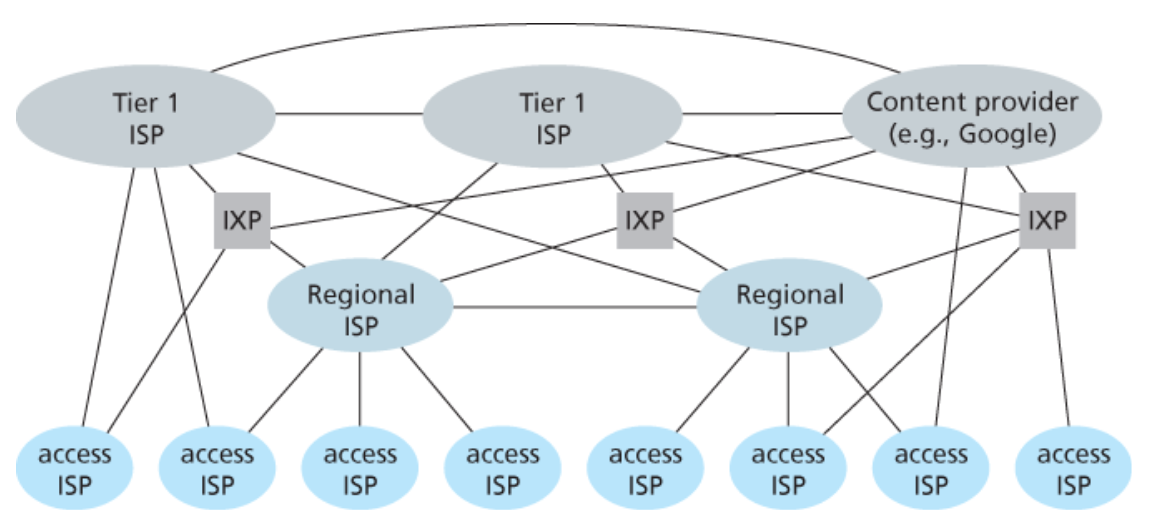
\includegraphics[width=0.7\textwidth]{img/internet/Estructura-Internet-ISP.png}
    \caption{Ejemplo de estructura jerárquica de Internet}
    \label{fig:estructura_internet}
\end{figure}



Así, estos proporcionan a los usuarios finales el acceso a proveedores de contenido (CDN, por sus siglas en inglés), sitios web y otros servicios, los cuales también están conectados a la infraestructura de Internet.\\

% Para el correcto funcionamiento de Internet existen diferentes protocolos, sin embargo, los dos más importantes corresponden al Protocolo de Control de Transmisión (TCP) y el Protocolo de Internet (IP),conocidos colectivamente como TCP/IP. El desarrollo de estos estandares los lleva acabo el Internet Engineering Task Force (IETF) \cite{IETF}, y los documentos se conocen como Requests for Comments (RFCs).

\section{Sistemas Autónomos} \label{sec:sistemas_autonomos}

En la estructura de Internet, un Sistema Autónomo (AS) consiste en un conjunto de routers y enlaces de comunicación que comparten una política de enrutamiento común. Estos son operados de forma independiente por organizaciones, como ISPs , universidades, empresas, entre otras.\\



\begin{figure}[h]
    \centering
    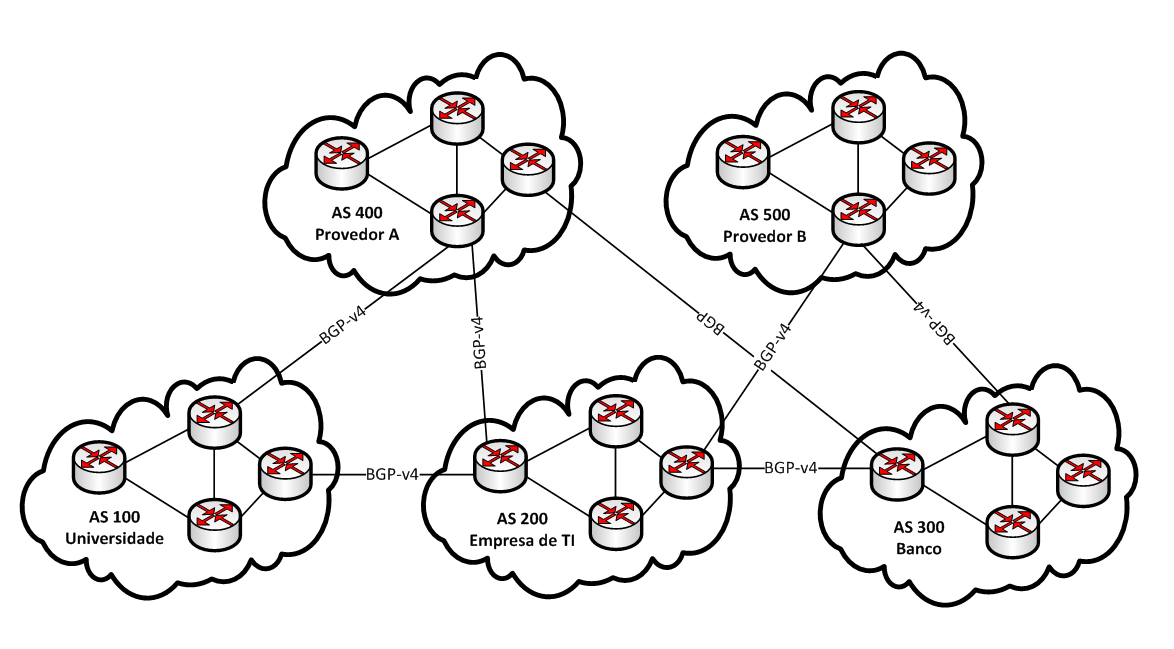
\includegraphics[width=0.5\textwidth]{img/internet/topologiaBGP.png}
    \caption{Ejemplo de topología a nivel de Sistemas Autónomos.}
    \label{fig:topologia-ASes}
\end{figure}

Los ASes utilizan el protocolo BGP para intercambiar información de enrutamiento entre ellos y así lograr una conexión global entre ASes y, por ende, en Internet. Las conexiones entre los Ases pueden ser de tipo cliente-proveedor, peer-to-peer o sibling-to-sibling, pero están influenciadas por acuerdos comerciales. Bajo estos acuerdos, podemos crear un grafo de la infraestructura de Internet, donde los nodos son los ASes y las aristas son las conexiones entre ellos. Cabe destacar que, en este caso, una conexión no implica necesariamente el intercambio de tráfico entre los ASes conectados, ya que el enrutamiento está controlado por BGP, un protocolo de enrutamiento basado en políticas~\cite{InferringASRelatioships2001}.\\

En la Figura~\ref{fig:topologia-ASes} se observa una serie de Sistemas Autónomos: proveedores de servicios (AS 400 y AS 500), una universidad (AS 100), una empresa de TI (AS 200) y un banco (AS 300). Cada uno está compuesto por múltiples routers, donde únicamente los routers de borde de cada AS se conectan mediante sesiones BGP con otros Sistemas Autónomos.\\

Otro concepto importante para entender la estructura de Internet son los Internet Exchange Points (IXPs). Estos corresponden a puntos de interconexión, donde múltiples ASes se conectan, y establecen conexión con otros ASes sin necesidad de estar directamente conectados.

Más información sobre los Sistemas Autónomos y los IXPs puede encontrarse en los Anexos \ref{sec:sistemas_autonomos_section} y \ref{sec:ixp_section}, respectivamente.


\section{Ruteo}


Antes de introducir el protocolo BGP, debemos entender brevemente el \textbf{ruteo}.\\


El \textbf{ruteo} es el proceso mediante el cual se selecciona el camino que seguirá un paquete dentro de una red para llegar a su destino final. 
El camino que sigue un paquete se elige según la información de las \textbf{{tablas de enrutamiento} (\textbf{RIBs}) de los routers y la información contenida en los \textbf{encabezados de los paquetes}}, donde se indica el destino final.\\



Cuando un paquete llega a un \textbf{router}, se consulta en la \textbf{tabla de enrutamiento} la dirección final para obtener el próximo router o punto de red al cual se debe dirigir el paquete.\\



Por ejemplo, cuando un usuario accede a una página web desde su hogar, los paquetes viajan desde el servidor que aloja la página web hasta el router de su casa. 
Este router luego examina el encabezado del paquete para identificar el destino final, consulta su tabla de enrutamiento y lo reenvía al siguiente punto de la red. 
Este nuevo router intermedio repite el proceso hasta que el paquete alcanza su destino final.\\



Existen dos tipos de enrutamiento: \textbf{estático} y \textbf{dinámico}. 
El enrutamiento \textbf{estático} implica el uso de tablas fijas, las cuales deben ser modificadas manualmente para cambiar su configuración. 
Por otro lado, en el enrutamiento \textbf{dinámico}, los routers se encargan de actualizar las tablas de enrutamiento en tiempo real, ajustándolas según las condiciones de la red.\\
%Este proceso se lleva a cabo mediante los protocolos de enrutamiento.\\


Dicho esto, podemos representar el \textbf{grafo de Internet} como el grafo \textbf{$G = (N, E)$}, donde $N$ corresponde al conjunto de \textbf{ASes} y $E$ al conjunto de \textbf{aristas} entre estos, las cuales representan si un paquete en Internet puede ocupar dicho enlace para llegar de un punto a otro.

\section{Border Gateway Protocol (\textbf{BGP})}

Como se mencionó, existen dos tipos de ruteo: estático y dinámico. 
BGP~\cite{RFC-BGP} pertenece al tipo dinámico; este se encarga de analizar todas las posibles rutas a los diferentes destinos y seleccionar la mejor ruta. 
Luego, comparte esta información con sus ASes vecinos, quienes a su vez repiten el proceso. 
Así, cada Sistema Autónomo (AS) genera caminos hacia los distintos prefijos de Internet y, cuando ocurren cambios en la red, BGP también se encarga de actualizar las rutas mediante el intercambio de mensajes \textit{UPDATE}.\\


BGP comienza una vez que se ha establecido la conexión TCP entre los pares BGP, estos intercambian mensajes \textit{OPEN} para confirmar los parámetros de la sesión. Luego, envían un mensajes \textit{KEEPALIVE} para confirmar la conexión.\\

La información que se intercambia en primera instancia consiste en una porción de la tabla de información de BGP, llamada \textit{Adj-RIB-Out}, la cual está filtrada de acuerdo a las políticas locales de exportación hacia los diferentes ASes. A medida que esta tabla va cambiando, se envían actualizaciones incrementales mediante mensajes \textit{UPDATE}. \\
Además, para asegurar que la conexión sigue activa, los pares BGP intercambian cada cierto tiempo mensajes \textit{KEEPALIVE}.\\

En caso de que se detecte algún tipo de error durante la conexión, se envía un mensaje \textit{NOTIFICATION} el cual indica el tipo de error y tras su envío la conexión BGP se cierra y todas las rutas aprendidas en la sesión son eliminadas.\\

La Figura~\ref{fig:Funcionamiento-BGP} muestra cómo BGP propaga la información de ruteo entre distintos AS.
Cada sistema autónomo anuncia la dirección de destino a sus pares, en este caso específico el AS 64503 anuncia su dirección a sus pares $64502$ y $64504$, quienes a su vez anuncian la dirección a sus pares, modificando el \textit{AS\_PATH}  a medida que la información se propaga. Finalmente, el AS 64501 recibe estos anuncios y, basándose en la información acumulada, determina la mejor ruta para alcanzar la red del AS 64503.\\


\begin{figure}[H]
    \centering
    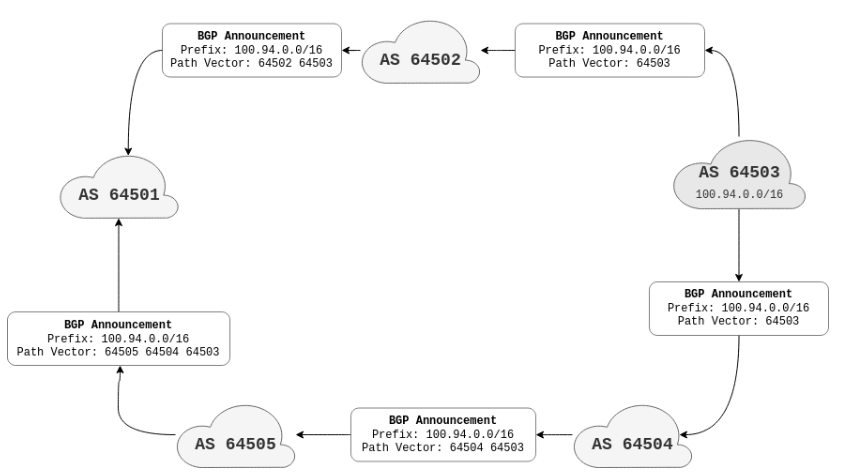
\includegraphics[width=0.7\textwidth]{img/internet/BGPFuncionamiento.png}
    \caption{Ejemplo de propagación de mensajes UPDATE. En este caso AS 6453 comienza anunciando su dirección a sus pares.}
    \label{fig:Funcionamiento-BGP}
\end{figure}


Más información sobre los tipos de mensajes del protocolo puede encontrarse en el Anexo \ref{sec:anexo_mensajes_bgp}.

\subsection{\textbf{BGP} Routing Information Base (RIB)}

Otro concepto importante son las tablas RIBs. A partir de las cuales se extrajo la información para construir el grafo de Internet y la arista que conectan a los ASes en este trabajo.\\

Cuando se utiliza BGP, los routers BGP reciben mensajes \textit{UPDATE} de sus vecinos, los cuales son analizados y filtrados según las políticas locales de ruteo del AS, para luego anunciar las rutas seleccionadas a sus vecinos. Para esto, BGP utiliza una base de datos denominada Routing Information Base (RIB), que se compone de tres partes:\\

\begin{itemize}
    \item \textbf{Adj-RIB-In:} Almacena la información de ruteo de los mensajes \textit{UPDATE} recibidos de los vecinos BGP.
    \item \textbf{Loc-RIB:} Contiene la información de ruteo local, es decir, las mejores rutas seleccionadas para cada dirección.
    \item \textbf{Adj-RIB-Out:} Guarda la información seleccionada por el router para ser anunciada a sus pares. Consiste en la información de \textit{Loc-RIBs} luego de ser aplicadas las políticas internas de ruteo. Esta es la información que se incluye en los mensajes \textit{UPDATE}.
\end{itemize}

El flujo de información en BGP y el proceso de toma de decisiones de rutas se realiza de la siguiente manera:
primero, se reciben los mensajes \textit{UPDATE} de los vecinos, los cuales se almacenan en la \textit{Adj-RIB-In}, una entrada por cada vecino. Luego, se evalúa el grado de preferencia de cada ruta almacenada en la \textit{Adj-RIB-In}. En base en esta evaluación, se seleccionan las mejores rutas para cada destino y se instalan en la \textit{Loc-RIB}. Finalmente, la información contenida en la \textit{Loc-RIB} se transfiere a la \textit{Adj-RIB-Out} para ser anunciada a los vecinos BGP, siguiendo las políticas de ruteo locales. Este flujo de información se conoce como el proceso de decisión BGP.\\

Es importante destacar que las bases de datos que almacenan la información de rutas BGP no son lo mismo que la tabla de ruteo de un router, que es la que el router utiliza para realizar el forwarding de los paquetes. Las rutas almacenadas en la RIB deben cumplir con ciertos criterios, definidos por el software o el proveedor del router, para ser agregadas a la tabla de ruteo.\\


\section{Redes Neuronales}

A continuación, se presenta una introducción básica a las Redes Neuronales, para luego pasar al funcionamiento y arquitecturas básicas  de las Redes Neuronales de Grafos, las cuales fueron utilizadas en el desarrollo de esta tesis.\\

Una Red Neuronal es un modelo computacional compuesto de neuronas (perceptrones), dispuestas en capas y conectadas entre sí con el fin de aprender patrones mediante el intercambio de información ponderada por pesos. Estos pesos se ajustan en base a los datos de entrada, asignando valores en función del reconocimiento de patrones, que permiten una salida esperada.\\


\begin{figure}[h]
    \centering
    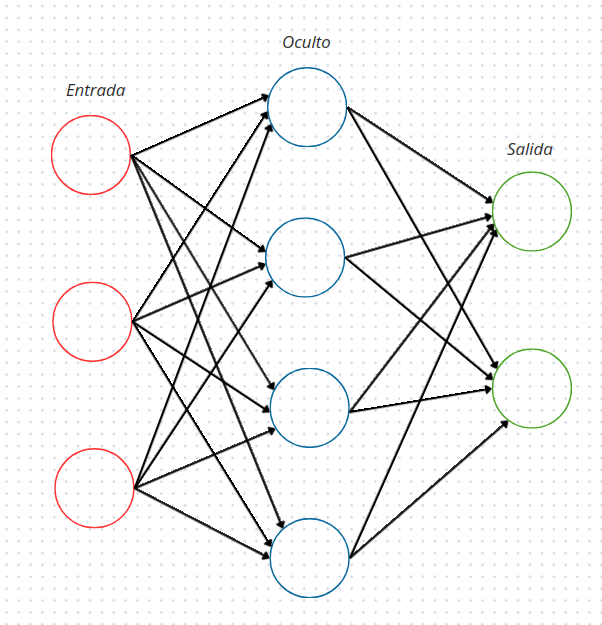
\includegraphics[width=5cm]{img/redesNeuronales/red_neuronal.png}
    \caption{Arquitectura básica de una Red Neuronal Fully Connected de una capa.}
    \label{fig:fully-connected}
\end{figure}


En una Red Neuronal, cada unidad toma entradas, las pondera por separado, suma los valores y pasa esta suma a través de una función para producir una salida, la cual es compartida con otras neuronas a las cuales está conectada.\\


El perceptrón, que funciona como una representación matemática de una unidad básica en la Red, realiza cálculos para determinar tendencias en los datos de entrada, asignándole diferentes pesos a cada valor de entrada en base a patrones entre los datos para realizar tareas específicas.\\


Un perceptrón está compuesto por cuatro elementos distintivos (Figura \ref{fig:perceptron}), i) los valores de entrada definidos como $x_i, x_{i+1} , ... , x_{n-1}, x_n$ donde cada $x_j$ corresponde a un vector de tamaño d, ii) los pesos definidos como  $w_j \in \mathbb{W}^{n \times d}$ donde $\mathbb{W}$ corresponde a la matriz de pesos los cuales son ajustados durante la etapa de entrenamiento de la Red, iii) la suma $z = \sum_{j=1}^{d} w_j x_j + b$ y iv) la función de activación, la cual establece un umbral de salida para evitar que los valores de salida se disparen. Esta función de activación permite incluir más capas y, por ende, mayor complejidad en las arquitecturas de redes que se construyan. Las funciones de activación tienen la capacidad de mejorar el aprendizaje de patrones en los datos~\cite{activation-function}.
Algunas de las funciones de activación comúnmente empleadas incluyen la Sigmoide, la Tangente Hiperbólica (tanh), la Rectified Linear Unit (ReLU) y la  Leaky ReLU.\\


\begin{figure}[h]
    \centering
    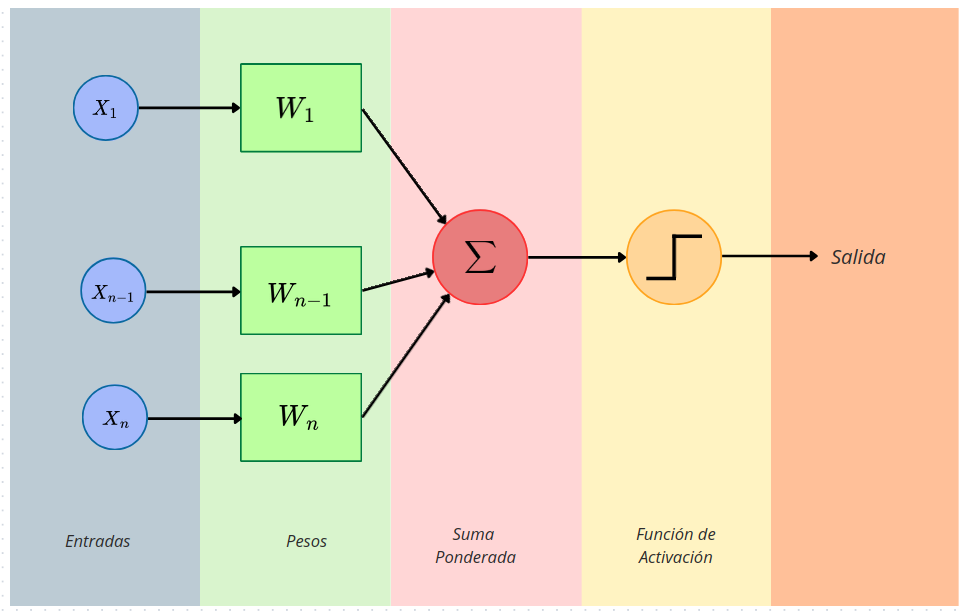
\includegraphics[width=10cm]{img/redesNeuronales/perceptron.png}
    \caption{ Estructura general de un perceptrón. }
    \label{fig:perceptron}
\end{figure}


La técnica comúnmente utilizada para el entrenamiento de Redes Neuronales es el \textit{backpropagation},
que tiene como objetivo ajustar los pesos de los parámetros de la Red para minimizar la función de pérdida~\cite{back-propagation}. Esta función cuantifica la diferencia entre las predicciones hechas y los valores reales. Una vez que se ha calculado la pérdida, el proceso de optimización se centra en modificar los pesos para mejorar la precisión general de la Red.\\

Durante el entrenamiento de las Redes Neuronales, se emplea el descenso de gradiente, un método que implica el cálculo de la derivada de la función de pérdida con respecto a los pesos de la Red. Este cálculo determina la dirección y magnitud en la que los parámetros de un modelo deben ser ajustados para minimizar la función de pérdida. Por ende, es fundamental que esta función sea continua y derivable.
En problemas de regresión, se suele utilizar funciones como el Mean Squared Error y Mean Absolute Error, mientras que en problemas de clasificación, destaca la Cross-Entropy Loss. \\


\section{Graph Neural Network (GNN)}

Las GNN son una arquitectura de redes neuronales especialmente diseñada para realizar predicciones basadas en datos representativos de grafos~\cite{scarselli_graph_2009}. A diferencia de las Redes Neuronales convencionales, las GNNs reciben datos en forma de tensores que pueden representar nodos, atributos de nodos, aristas y atributos de aristas.\\

% Existen diferenets enfoques, dependiendo de la tarea de aprendizaje que se quiere llevar a cabo, estos son:

% - Nivel de nodo: Incluye tareas como clasificación, regresión y clustering de nodos. Se realizan inferencias a partir de las conexiones con otros nodos. 


% - Nivel de  aristas: Se abordan tareas de clasificación y predicción de aristas. Por ejemplo, determinar la existencia de una relación entre dos nodos.

% - Nivel de grafo: Se encuentran tareas de clasificación, regresión y matching de grafos para las cuales el modelo debe ser capaz de aprender una representación para el grafo completo.


Las GNN tienen una serie de ventajas sobre las Redes Neuronales convencionales cuando se trabaja con datos de grafos. En contraste con los modelos tradicionales, las GNN aprovechan las relaciones entre las entidades que conforman los datos de entrada a el modelo. Estas relaciones pueden incluir aspectos como orden, jerarquía, dependencias o relaciones de otro tipo que son comunes en grafos y se representan a través de las aristas que conectan los nodos.\\

En cuanto a la adaptabilidad a variaciones en el tamaño de entrada, las Redes Neuronales convencionales requieren que los datos de entrada mantengan un mismo tamaño. Para ello, recurren a técnicas como padding o broadcast, los cuales no tienen efectos significativos en el desempeño de los modelos. Las GNNs, por su parte, ofrecen flexibilidad para adaptarse a distintos tamaños de entrada~\cite{GCN}.\\

Otro motivo para optar por GNNs es su capacidad para manejar el isomorfismo de los grafos, es decir dos grafos pueden lucir diferentes, pero ser estructuralmente iguales. Un modelo tradicional trataría ambos grafos como si fuesen datos diferentes, sin embargo, no lo son. Esto es comparable a lo que sucedería si se le presenta como entrada dos imágenes donde una se encuentra invertida. Es por esta razón que no se puede trabajar directamente con una matriz de adyacencia en una Red Feed Forward, ya que es sensible a estos cambios. Las GNNs utilizan técnicas que son invariantes ante permutaciones, lo que permite trabajar con el isomorfismo en grafos.\\

Finalmente, el último desafío radica en que la estructura de un grafo no puede ser reducida a un espacio euclidiano, y su conceptualización no puede limitarse a una distancia euclidiana~\cite{EuclideanGNN}. A diferencia de Redes Neuronales que trabajan, por ejemplo, con imágenes, las cuales pueden ser interpretadas como un grafo, la representación de la información se puede entender en términos de píxeles en un espacio bidimensional. \\



\subsection{Message Passing Neural Networks (MPNN)}
    
Es la arquitectura de Red Neuronal para grafos más utilizada. Su funcionamiento radica en la idea de que cada nodo en un grafo puede intercambiar información con sus vecinos de manera que cada nodo podrá actualizar su representación en base a la información acumulada por su entorno.\\


La información se propaga entre nodos a través de mensajes. Cada nodo envía mensajes a sus nodos vecinos y recibe mensajes de ellos. Estos mensajes pueden contener información sobre el nodo emisor y se utilizan para actualizar la representación del nodo receptor~\cite{mpnn}.\\


Se emplea un mecanismo denominado \textit{message passing}, el cual consta de tres pasos:
\begin{enumerate}
    \item Propagación de mensajes entre nodos: Cada nodo envía un mensaje que contiene su representación actual a sus nodos vecinos.
    \item Aplicación de una función de agregación: Luego de la propagación de mensajes, se aplica una función de agregación para combinar la información recibida de los nodos vecinos.
Esta función puede adoptar diversas formas como la suma o la media.
    \item Actualización de la representación: La representación de cada nodo se actualiza mediante la información agregada proveniente de sus nodos vecinos, así como a partir de su representación previa.
\end{enumerate}

En Figura~\ref{fig:pipelineMP}, se presenta el comportamiento de una capa de MPNN para un nodo. El proceso inicia con el envío de un mensaje M por parte de cada nodo vecino de $B$. $B$  recibe estos mensajes y los agrega mediante una operación generando una representación $A$. Finalmente, el nuevo estado del nodo $B$ se calcula mediante una última función que toma el valor $A$ y su propia representación para crear su nueva descripción $U$.\\

\begin{figure}[h]
    \centering
    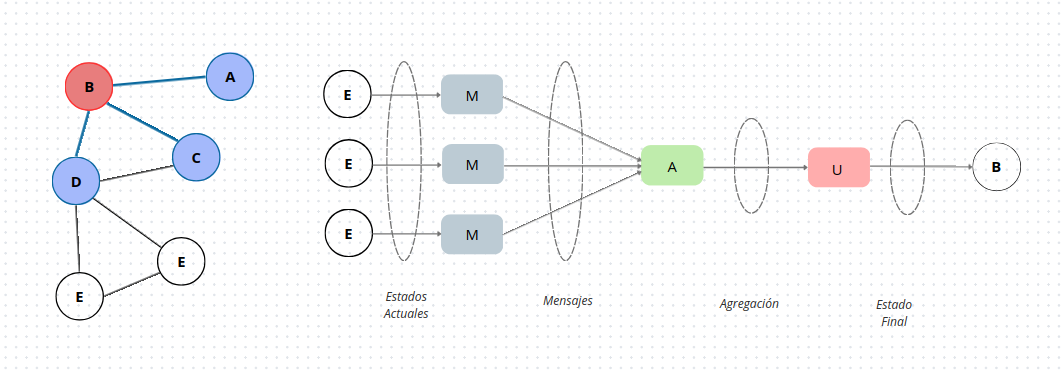
\includegraphics[width=0.7\textwidth]{img/gnn/MPNN.png}        \caption{Flujo de Message passing para un nodo del grafo.}
    \label{fig:pipelineMP}
\end{figure}

\subsection{Graph Convolution Network (GCN)}

Es un tipo específico de MPNN, donde se utilizan convoluciones de grafos para agregar información de los nodos adyacente de un nodo en un grafo. \\

La operación de convolución en el grafo produce la suma normalizada de las características de los nodos vecinos~\ref{ecu:GCN-foormula}. Esta normalización garantiza que la información agregada sea ponderada correctamente, es decir, evitar que un nodo con gran cantidad de vecinos tenga una representación desproporcionada y que luego tenga una influencia mayor en la representación otros nodos en las siguientes capas.\\

La notación de los embeddings de los nodos $h^{(l+1)}_i$ en la capa $l+1$ de la red está dado por: \\



\begin{equation}
    h^{(l+1)}_i = \sigma \left( b^{(l)}_i + \sum_{j \in N(i)} \frac{1}{c_{ji}} h^{(l)}_j W^{(l)} \right)
    \label{ecu:GCN-foormula}
\end{equation}
\\



Donde $\sigma$ se define como la función de activación, $h^{(l)}$ la matriz de características de los nodos en la capa $l$, $W^{(l)}$ la matriz de aprendizaje de pesos, con dimensionalidades dada por el tamaños de atributos entrantes y $c_{ij}$ el termino de normalización.\\


Es así como GCN permite la creación de embeddings para los nodos de un grafo dada la matriz de adyacencia de este, lo que quiere decir que debe conocer el grafo completo para poder realizar la tarea de aprendizaje. Este es un enfoque transductivo, en contraste a otros enfoques inductivos como GraphSAGE.\\

\subsection{Graph Attention Network (GAT)}

Otra variante de MPNN son las Graph Attention Networks (GAT). A diferencia de una Red Neuronal de Convolución, GAT incorpora un mecanismo de atención que permite que cada nodo pondere de forma diferenciada, indicando la importancia de las representaciones de cada vecino para la actualización de las características de un nodo~\cite{GAT}.\\

Los coeficientes se calculan por un mecanismo el cual calcula un puntaje para cada par de nodos. Luego estos puntajes se normalizan por medio de la función softmax (Figura~\ref{fig:calculoGAT}).\\

Así tenemos:\\


\begin{equation}
   z^{(l)}_{i} = W^{(l)} \mathbf{h}^{(l)}_i
   \label{ecu:paso-1-gat}
\end{equation}


\begin{equation}
   e^{(l)}_{ij} = \text{LeakyReLU}(\mathbf{a}^{(l)T}(\mathbf{z}^{(l)}_i || \mathbf{z}^{(l)}_j))
   \label{ecu:paso-2-gat}
\end{equation}


\begin{equation}
   \alpha^{(l)}_{ij} = \frac{e^{(l)}_{ij}}{\sum_{k \in N(i)} \exp(e^{(l)}_{ik})}
   \label{ecu:paso-3-gat}
\end{equation}


\begin{equation}
    h^{(l+1)}_i = \sigma \left(\sum_{j \in N(i)} \alpha^{(l)}_{ij} z^{(l)}_j\right)
    \label{ecu:paso-4-gat}
\end{equation}
\\

Donde~\ref{ecu:paso-1-gat} es la transformación lineal del embedding de la capa anterior $h^{(l)}_i$ con $ W^{(l)}_i$ una matriz de pesos entrenable.\\

La ecuación~\ref{ecu:paso-2-gat} calcula un puntaje de atención entre dos vecinos.  Primero, concatena los embeddings $z$ de dos nodos. Luego realiza el producto punto entre este y una matriz entrenable $a^{(l)}$  y aplica una función LeakyReLU al final.\\

En~\ref{ecu:paso-3-gat} se aplica una función softmax, con el objetivo de normalizar los puntajes de atención en las aristas entrantes de cada nodo.\\

Finalmente, en la ecuación~\ref{ecu:paso-4-gat}, al igual que en GCN, se lleva a cabo la agregación de los nodos vecinos, pero en este caso, se escala por el puntaje de atención. Se utiliza  $\sigma$ como la función de activación que se aplicará a la capa.\\

\begin{figure}[h]
    \centering
    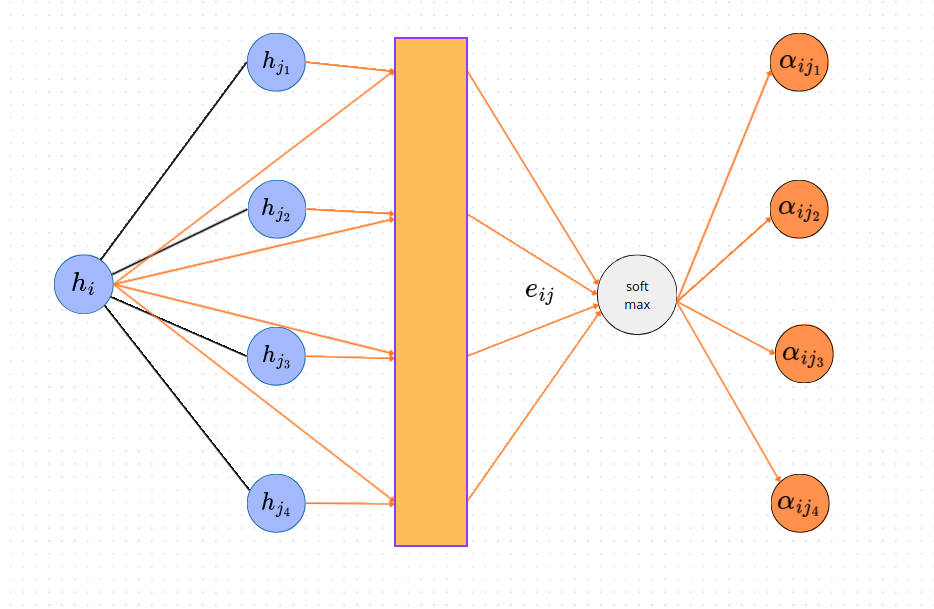
\includegraphics[width=10cm]{img/gnn/GAT.png}
    \caption{Pipeline del mecanismo de cálculo de las ponderaciones para una GAT.}
    \label{fig:calculoGAT}
\end{figure}



\subsection{GraphSAGE (SAmple and aggreGatE)}

Es un framework de aprendizaje inductivo el cual nos permite aprender representaciones de los nodos de un grafo. A diferencia de los enfoques anteriores los cuales son inherentemente transductivos donde se crean las representaciones de los nodos por medio de la recolección de la información de todos sus nodos vecinos, utilizando factorización de matrices, GraphSAGE aprende a crear las representaciones de sus nodos, es decir graphSAGE utiliza las características de nodos de su vecindario y la topología para aprender una función que genera los embeddings en base a un muestreo de nodos vecinos. Ayudado de esta forma a generalizar sobre nodos no vistos naturalmente~\cite{GraphSAGE}. \\

GraphSAGE no necesita de todos sus vecinos durante el entrenamiento para crear una representación del mismo, sino que a través de un subconjunto de estos aprenderá a crear un embedding, que representa su rol local y global en un grafo.\\
 
Que sea inductivo significa que puede crear embeddings para nodos no vistos durante el entrenamiento. Es decir, no necesita conocer todo el grafo ni todos los nodos para crear estas representaciones. 
Este enfoque es útil principalmente a la hora de trabajar con grafos dinámicos, batching/sampling, etc. Representando así a nodos en un vector de baja dimensionalidad y generalizándolo luego para nodos no vistos.\\

El proceso de creación de embeddings para los nodos del grafo está dado por las siguientes ecuaciones:

\begin{equation}
    h^{(l+1)}_{N(i)} = \operatorname{aggregate}\!\left(\left\{ h^l_j \mid \forall j \in N(i)\right\}\right)
    \label{ecu:graphsage-formula-1}
\end{equation}


\begin{equation}
    h^{(l+1)}_i = \sigma\!\left(W \cdot \operatorname{concat}\!\left(h^l_i, h^{(l+1)}_{N(i)}\right)\right)
    \label{ecu:graphsage-formula-2}
\end{equation}

\begin{equation}
    h^{(l+1)}_i = norm(h^{(l+1)}_i)
    \label{ecu:graphsage-formula-3}
\end{equation}

Donde $h^{(l+1)}_{N(i)}$ de~\ref{ecu:graphsage-formula-1} representa las características de los nodos vecinos de un nodo $i$ en la capa $l+1$ el cual, a través de una función de agregación combina estos nodos vecinos. Esta función de agregación puede ser el promedio, suma, lstm u otras.
Luego tenemos $h^{(l+1)}_i$ correspondiente a la concatenación de la representación anterior del nodo $i$ y la de las características de nodos vecinos de la capa $l+1$, correspondiente a lo previamente calculado.
Finalmente tenemos $norm(h^{(l+1)}_i)$ la cual se encarga de normalizar las características del nodo $i$ en la capa $l+1$.\\

La Figura~\ref{fig:graphsage} ilustra el proceso de creación de las representaciones de los nodos. Dado primero 1) por la selección de un número fijo de vecinos de un nodo, 2) luego la agregación y concatenación de las características de estos nodos al nodo destino junto con normalización, y finalmente 3) el paso de predicción y ajuste de valores de los pesos de la red. \\

\begin{figure}[h]
    \centering
    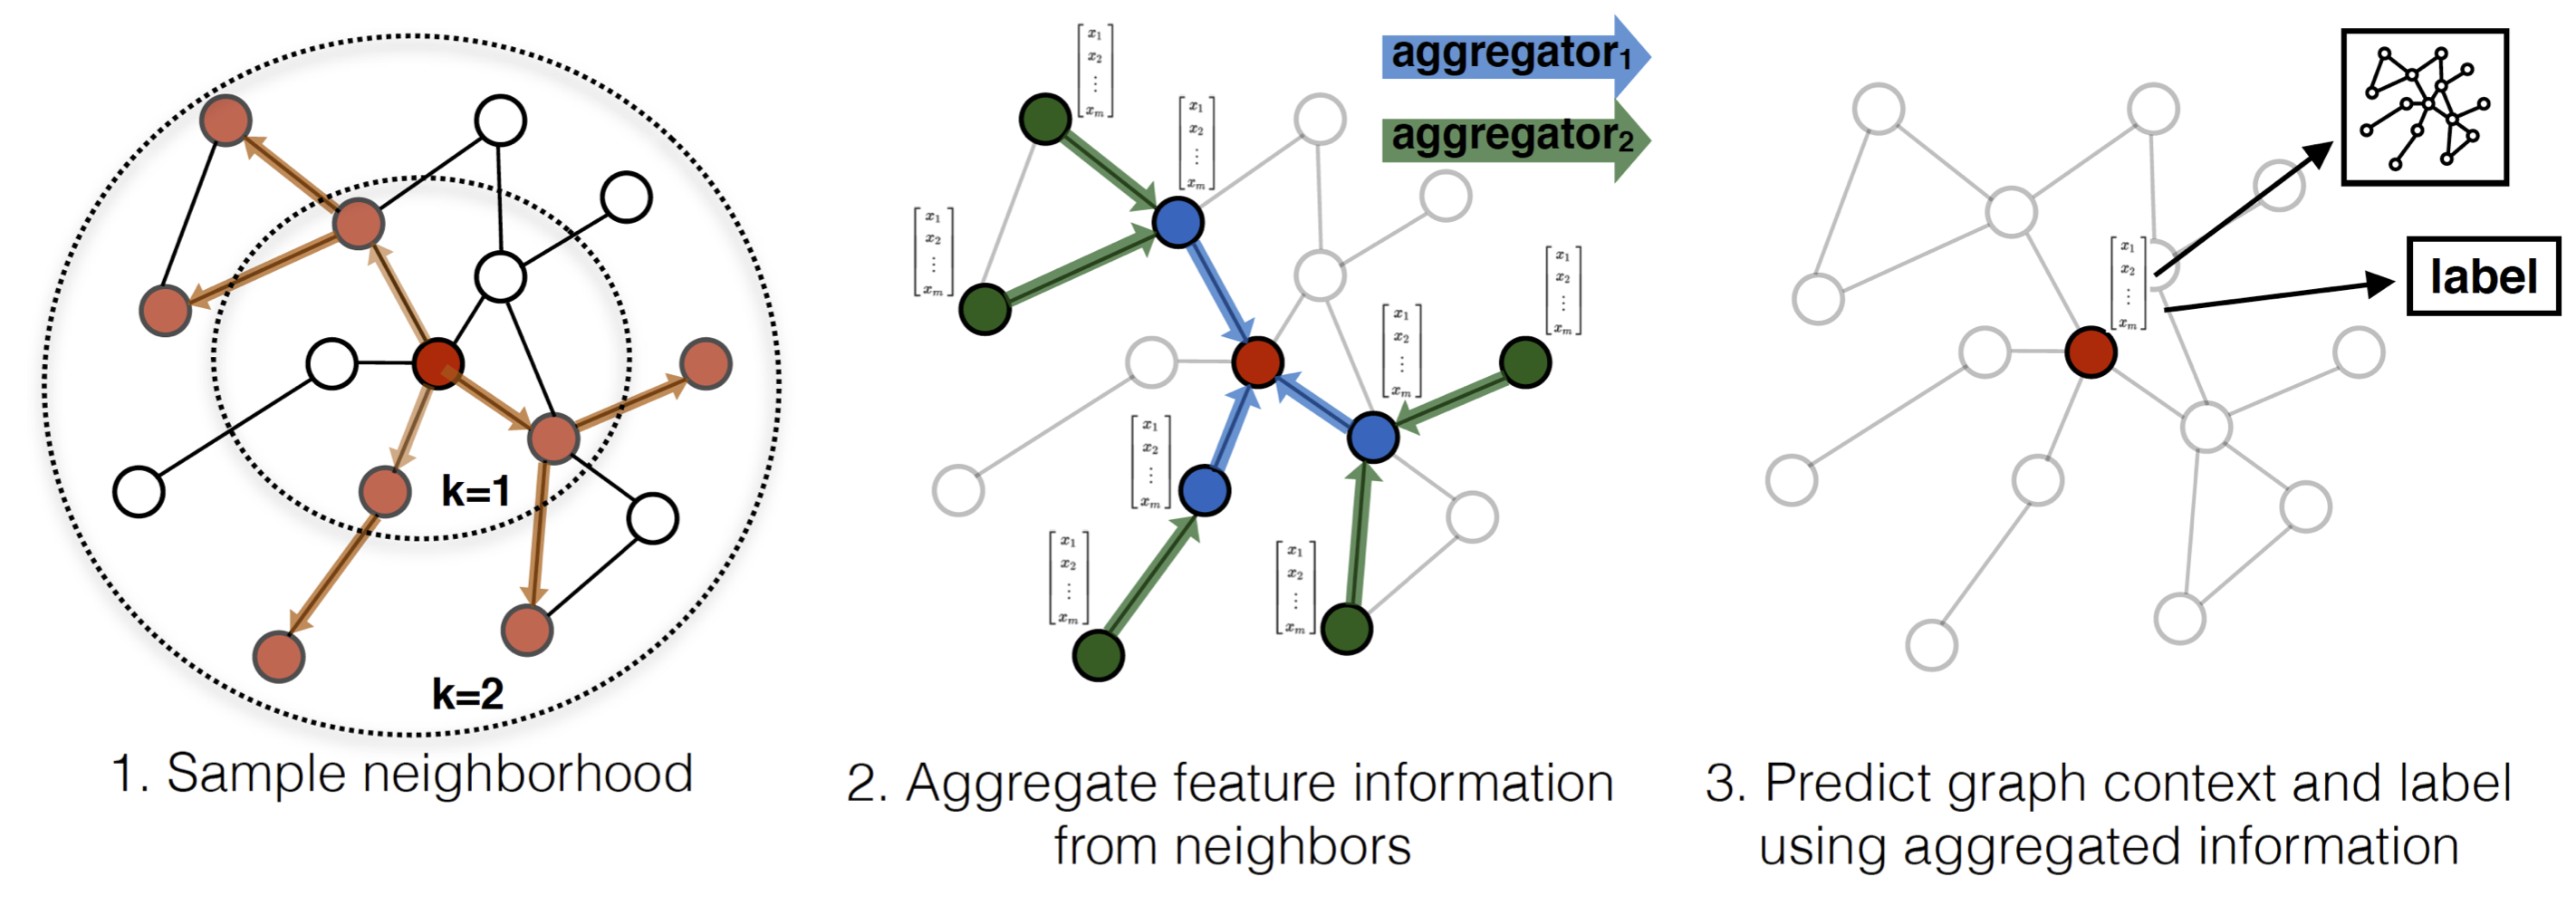
\includegraphics[width=0.7\textwidth]{img/gnn/sample_and_agg.png}
    \caption{Proceso de creación de representaciones de nodos con GraphSAGE.
    Fuente https://snap.stanford.edu/graphsage/}
    \label{fig:graphsage}
\end{figure}



\chapter{Trabajo Relacionado}


\section{Tipos de Relaciones entre Sistemas Autónomos}

El ruteo de los paquetes que transitan por Internet no depende únicamente de la infraestructura física, sino también de las políticas de enrutamiento establecidas entre los Sistemas Autónomos.  Estas políticas están  principalmente influenciadas por las relaciones comerciales entre los ASes~\cite{computing-observed-autonomous-system-relationships-in-the-internet}.\\

Estas relaciones son las que determinan por dónde fluye el tráfico entre los ASes, ya que cada uno define sus políticas basándose en sus necesidades y modelo de negocio. Existen dos tipos principales de relaciones entre los Sistemas Autónomos: customer-to-provider (C2P), donde un cliente paga a un proveedor para acceder a partes del internet que el mismo no alcanza, y peer-to-peer (P2P), donde dos ASes intercambian tráfico destinado a sus respectivos clientes de manera mutua y sin pago de por medio.\\


Gao~\cite{InferringASRelatioships2001} fue la primera en estudiar las relaciones entre los ASes. En su estudio, sentó las bases para abordar su estudio al proponer una forma de representar las relaciones en Internet mediante un grafo parcialmente dirigido (Figura~\ref{fig:tipos-as-rel-chashflow}), donde los nodos representan los Ases y las aristas representan las relaciones entre ellos. En este modelo, las relaciones de customer-to-provider se representan mediante una arista dirigida. Estos acuerdos son más comunes en los bordes del grafo de Internet, donde la topología estaría compuesta  principalmente por ``hojas'', las cuales están principalmente preocupadas por la entrega de su propio tráfico. En contraste, en el núcleo de Internet, la topología consiste en redes densamente interconectadas~\cite{SurveyInterconnectionAgreements}.\\



Conocer las relaciones entre los ASes es de vital importancia, ya que permite entender el comportamiento del tráfico de Internet, detectar posibles ataques y fallos en la red, y optimizar el ruteo de los paquetes. Sin embargo, estas no son de acceso público, por lo que inferir estas relaciones es un problema de gran relevancia en la actualidad. 

A través de las rutas anunciadas mediante BGP, es posible inferir el tipo de relación entre los ASes. \\

La inferencia de estas relaciones ha sido un tema de estudio durante las últimas dos décadas, en las cuales se han propuesto diferentes algoritmos para resolverlo, siendo la mayoría de estos métodos heurísticos   %FIXME: Agregar referencia de los metodos heuristicos InferringASRelatioships2001 \cite{computing-observed-autonomous-system-relationships-in-the-internet} .
utilizando los datos públicos de enrutamiento BGP, como tablas de enrutamiento (RIBs) y anuncios BGP.\\

Gao presentó un primer algoritmo basado en la idea de que el grado de un AS en el grafo suele ser mayor que el de sus clientes, mientras que los ASes peers tienden a tener un grado similar~\cite{InferringASRelatioships2001}. Su método también incorporó el concepto de \textit{valley-free} (VF) en los caminos de enrutamiento.
El concepto de \textit{valley-free} establece que una ruta consistirá en cero o más enlaces C2P, seguido de cero o un 
enlace de peering, y luego cero o más enlaces P2C.

Esta propiedad captura los incentivos económicos que hasta cierto punto determinan el tráfico entre los ASes, ya que un AS no anunciará las rutas aprendidas de un peer o proveedor, eso implicaría el tránsito gratuito de tráfico, lo que aumentaría los costos de infraestructura sin generar beneficios a cambio~\cite{ProbLink}.\\

\begin{figure}[h]
    \centering
    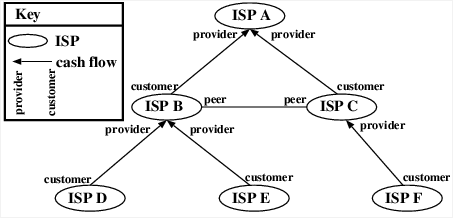
\includegraphics[width=0.7\textwidth]{img/internet/pyramid.png}
    \caption{Tipos de relaciones entre ASes. Fuente https://www.caida.org/catalog/datasets/as-relationships/}
    \label{fig:tipos-as-rel-chashflow}
\end{figure}


Un ejemplo es la Figura \ref{fig:tipos-as-rel-chashflow}, donde el ISP~D le paga al ISP~B para poder acceder al ISP~F, lo que define que tengan una relación del tipo customer-provider. Por otro lado, los ISPs~B y C comparten una relación peer-to-peer, lo que significa que no existe un acuerdo monetario entre ellos, ya que ambos se benefician mutuamente de la conexión. Sin embargo, en este tipo de relación solo se intercambia el tráfico proveniente de sus propios clientes, y no el de sus respectivos proveedores u otros Sistemas Autónomos con los que mantengan relaciones peer-to-peer.\\


\begin{figure}[h]
    \centering
    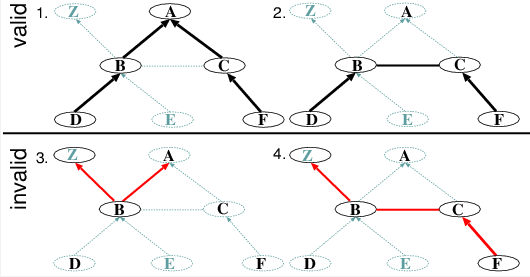
\includegraphics[width=0.7\textwidth]{img/internet/valid-invalid-paths.png}
    \caption{Ejemplos de dos caminos válidos y dos caminos inválidos según el concepto \textit{valley-free}. Fuente https://www.caida.org/catalog/datasets/as-relationships/}    \label{fig:valid-invalid-paths}
\end{figure}


Subramanian et al. \cite{CharacterizingIAS} formularon la tarea como un problema de optimización, definiéndolo como ``the type of relationship (ToR) problem''. Este problema consistía en etiquetar todas las aristas en un grafo de AS para maximizar el número de rutas VF en un conjunto de rutas BGP. Para simplificar el problema, excluyó las relaciones S2S (sibling-to-sibling), que son aquellas que entre dos Ases que pertenecen a un mismo dominio.\\


Se han realizado más estudios que han ido perfeccionando y profundizando en la comprensión del comportamiento de las relaciones entre ASes~\cite{ASRelationshipInferenceValidation,NearDeterministicInference,ProbLink,ComputingTypesRelationshipsBetweenAS,computing-observed-autonomous-system-relationships-in-the-internet}.\\

Luckie et al. \cite{ASRank} introdujeron el algoritmo \textit{AS-Rank} considerando el estado del arte para inferir relaciones C2P y P2P utilizando datos de BGP.
Ellos se basaron en tres supuestos: existe un clique de ASes proveedores de tránsito en la cima de la jerarquía de la topología de Internet, los clientes establecen relaciones con otros ASes con el fin de ser globalmente alcanzables y no existen ciclos de enlaces C2P para que el enrutamiento converja.
Así, introdujeron un nuevo algoritmo para inferir el ``cono de clientes'' de un AS, que es el conjunto de ASes que puede alcanzar utilizando enlaces P2C.\\
 
Por último, Shapira y Shavitt \cite{UnveilingtheTypeRelationshipBetweenAutonomousSystemsUsingDeepLearning} emplearon técnicas de Deep Learning para la tarea de clasificación.
Utilizaron BGP2Vec con el objetivo de crear representaciones de los Sistemas Autónomos y luego pasaron estos \textit{embeddings} 
aprendidos a una Red Neuronal Artificial, la cual se encargó de clasificar los tipos de relaciones entre pares de ASes, 
obteniendo una precisión del 95.2\%. Cabe destacar que el entrenamiento de esta Red Neuronal fue realizado con los datos inferidos del dataset \cite{CAIDAS-relationship}.\\

En nuestro caso desarrollamos esta tarea utilizando Redes Neuronales de Grafos, realizando un experimento similar al de Shapira y Shavitt \cite{UnveilingtheTypeRelationshipBetweenAutonomousSystemsUsingDeepLearning}, pero aplicando GNNs en lugar de una Red Neuronal tradicional. Para ello, primero crearemos un \textit{benchmark} utilizando algunos de los métodos de inferencia de relaciones entre ASes para luego realizar una comparación entre estas técnicas.\\

En el Anexo~\ref{sec:anexo_inferencia_relaciones_as} se presentan métodos que se han desarrollado a lo largo de los años para identificar las relaciones comerciales entre Sistemas Autónomos, junto con su descripción y funcionamiento.\\



\subsection{Importancia de inferir correctamente las relaciones entre Sistemas Autónomos}

Inferir correctamente las relaciones económicas entre Sistemas Autónomos es importante porque estas relaciones influyen directamente en las políticas de exportación de rutas, en la selección de caminos y, en consecuencia, en la estructura observable del enrutamiento interdominio. Una inferencia incorrecta puede llevar a interpretaciones erróneas sobre la jerarquía de Internet, la posición relativa de ciertas redes y la naturaleza de sus interconexiones.\\
% FIXME: Arrgelar el por q es importnat conocerlas para investigacion como route laks o esas cosa sy q no son publicas
Además, conocer estas relaciones permite analizar con mayor precisión la organización económica y topológica de Internet, estudiar fenómenos como la centralidad de ciertos ASes, la presencia de núcleos densamente conectados y la dependencia de redes periféricas respecto de proveedores de tránsito. Esta información también resulta relevante para tareas de simulación, modelado de resiliencia, análisis de seguridad y detección de anomalías, ya que muchas de estas aplicaciones dependen de supuestos sobre cómo fluye el tráfico entre ASes.\\

Por otra parte, dado que las relaciones comerciales no son observables directamente en la mayoría de los casos, su inferencia constituye una tarea fundamental para transformar observaciones parciales del enrutamiento en una representación más interpretable de la estructura de Internet.\\


\subsection{Repositorios de trazas BGP utilizados y sus limitaciones}

Los estudios sobre inferencia de relaciones entre Sistemas Autónomos suelen basarse en repositorios públicos de datos BGP, entre los que destacan \textbf{RouteViews} y \textbf{RIPE RIS}. Estas iniciativas recolectan tablas de enrutamiento (\textit{Routing Information Bases}, RIBs) y mensajes \textit{UPDATE} desde múltiples colectores distribuidos en distintos puntos de Internet. En conjunto con fuentes complementarias como \textbf{CAIDA AS Relationships} y \textbf{PeeringDB}, permiten construir una aproximación de la topología AS-level y enriquecerla con información adicional sobre relaciones y atributos de los ASes.\\

En esta tesis, RouteViews y RIPE RIS se utilizan como fuentes principales de rutas BGP observadas, mientras que CAIDA aporta un conjunto de relaciones utilizado como referencia y PeeringDB provee atributos adicionales de los Sistemas Autónomos. Esta combinación permite construir un grafo de Internet a nivel de AS y estudiar la tarea de inferencia desde una perspectiva comparable con trabajos previos.\\

Sin embargo, estas fuentes no entregan una visión completa de la topología real de Internet. Los datos BGP dependen de la ubicación y cantidad de colectores disponibles, y reflejan únicamente las rutas visibles desde esos puntos de observación. Por ello, la topología inferida a partir de estas fuentes debe entenderse como una aproximación observada y parcial del Internet interdominio.\\

\paragraph{Cobertura limitada de los \textit{vantage points}.}
Una limitación central de los repositorios públicos de rutas BGP es su cobertura incompleta. Cada colector observa únicamente una fracción de las rutas globales, determinada por los \textit{vantage points} o vecinos desde los cuales recibe información. En consecuencia, muchas conexiones entre ASes pueden no aparecer en los datos recolectados, especialmente enlaces de peering privado y relaciones \textit{peer-to-peer}, que suelen ser más difíciles de observar que las relaciones cliente--proveedor. Además, como BGP anuncia principalmente la mejor ruta disponible, enlaces alternativos o de respaldo pueden permanecer ocultos en las RIBs públicas. Por esta razón, el grafo construido a partir de estas fuentes no representa toda la conectividad real de Internet, sino solo la porción visible desde los puntos de observación disponibles.\\



\chapter{Metodología}

En este capítulo se describen los procedimientos que se llevaron a cabo a lo largo de este trabajo. El objetivo es presentar el flujo de desarrollo, el cual comienza con la obtención y preparación de los datos (Sección~\ref{sec:obtencion_datos_section}), continúa con la construcción de un \textit{benchmark} con métodos que se han desarrollado previamente para resolver el problema en cuestión (Sección~\ref{sec:Benchmark_section}), la construcción del grafo de Internet (Sección~\ref{sec:creacion_grafo_section}), y finaliza con el diseño de modelos basados en Redes Neuronales de Grafos (Sección~\ref{sec:gnn_section}).\\

A modo de recapitulación, el problema abordado en este trabajo de tesis consiste en la inferencia de los tipos de relaciones económicas que comparten los Sistemas Autónomos (AS) en la red de Internet, por medio del uso de Redes Neuronales de Grafo. Durante todo el desarrollo se utilizó el lenguaje de programación Python y, en particular, se utilizaron las bibliotecas de Pytorch~\cite{Pytorch} y DGL~\cite{DGL} (Deep Graph Library) para la implementación de las GNNs, NetworkX~\cite{networkx} para la creación y manipulación de grafos y las bibliotecas estándar para el manejo de datos y otras funciones de utilidad.\\

El desarrollo del proyecto está organizado en dos repositorios. El primero, dedicado al \textit{benchmark}~\cite{BenchmarkCode}, el cual contiene las implementaciones de métodos preexistentes para la tarea de inferencia de relaciones entre ASes, mientras que el segundo repositorio~\cite{gnnCode} se encuentra enfocado en la construcción de un grafo de Internet y la aplicación de modelos basados en GNNs, además de incluir otros experimentos complementarios realizados durante el estudio.\\

%-----------------------------------------------------------------------------------------------------------------------------------------------------------------------------------------------------

\section{Obtención de Datos} \label{sec:obtencion_datos_section}


\subsection{Fuentes de Datos}
% Importancia de datos y dedonde se saco
La obtención de datos fue una etapa fundamental en el trabajo, comenzando con la búsqueda de fuentes confiables y de acceso público para obtener información sobre la topología de Internet. Para esto, se revisaron trabajos relacionados con el área de redes y el protocolo BGP, estudiando las fuentes de datos utilizadas en dichos estudios. Este proceso permitió identificar los conjuntos de datos utilizados comúnmente, provenientes principalmente de las iniciativas: RIPE RIS~\cite{RIPE-RIS}, RouteViews Project~\cite{RouteViewsProject}, CAIDA~\cite{CAIDA} y PeeringDB~\cite{PeeringDB}.\\

% desaffio
%\subsection{Desafíos de acceso y organización}

\vspace{0.5cm}
Uno de los principales desafíos de esta etapa fue la forma en que los datos se encuentran 
%\seba{en la versión final hay que evitar que queden líneas sueltas al final o al inicio de cada página. mientras estemos en borrador, no nos preocupemos de esto, pero hay que considerarlo finalmente.} 
organizados en sus respectivas plataformas. En general, estas presentan una estructura poco clara, con escasa documentación. Esto dificultó inicialmente la comprensión del contenido y el uso de la información. Sin embargo, a medida que se profundizó en el estudio y se revisaron trabajos previos, fue posible familiarizarse con los datasets utilizados para el análisis y estudio de Internet y el protocolo BGP.\\


% Objetivo de cada una de las plataformas de datasets
La dificultad de comprensión de estas páginas radica principalmente en que muchos estudios e información se repetían de distintas formas. Sin embargo, esto se debe a que cada fuente responde a objetivos distintos. CAIDA~\cite{CAIDA} actúa como repositorio de datos y estudios en el área de redes. RouteViews Project~\cite{RouteViewsProject} (RV), por otro lado, se enfoca en el uso de colectores ubicados en lugares estratégicos de la infraestructura de Internet, ofreciendo así datos BGP ``crudos'' (RIBs y mensajes \textit{UPDATE}) útiles para reconstruir el estado de enrutamiento en instantes específicos. Por último, RIPE RIS~\cite{RIPE-RIS} también mantiene una red de recolectores, pero además ofrece otros proyectos de medición del Internet así como servicios en tiempo real y \textit{datasets} complementarios.
Más información específica sobre las fuentes de datos puede encontrarse en el Anexo~\ref{sec:anexo_recoleccion_datos_internet}.\\

Finalmente, es importante destacar que estas fuentes proporcionan una visión parcial de la topología de Internet. En particular, los datos BGP observados desde RouteViews y RIPE RIS dependen de la cantidad y ubicación de los colectores y \textit{vantage points} disponibles, por lo que no todos los enlaces existentes en la red quedan necesariamente reflejados en las rutas recolectadas. Esta limitación es especialmente relevante en el caso de enlaces \textit{peer-to-peer} y conexiones privadas, cuya visibilidad suele ser menor en repositorios públicos.\\

\subsection{Acceso a RIBs y Herramientas Utilizadas}

Con el objetivo de mantener consistencia entre los datos de entrada del \textit{benchmark} y los modelos basados en GNNs, se decidió trabajar exclusivamente con las tablas \textit{Routing Information Bases} (RIBs) provenientes de los colectores de \textbf{RIPE RIS} y \textbf{RouteViews}, en lugar de utilizar el atributo los mensajes \textit{UPDATE} del protocolo BGP. Cabe destacar que, en un comienzo, se evaluó utilizar este segundo enfoque; sin embargo, se optó por el uso de las RIBs con el fin de mantener una coherencia metodológica con los trabajos previos de esta tarea, los cuales utilizan estas tablas como fuente principal de información.
Las RIBs corresponden a \textit{snapshots} que los routers mantienen con información sobre las rutas que debe seguir un paquete en Internet para llegar a un prefijo de direcciones IPs. Cada ruta está compuesta por una secuencia de \textit{Autonomous System Numbers} (ASN), donde cada par adyacente de ASes en la secuencia representa la existencia de una conexión entre ellos en la red.\\
% %TODO: Arrgñarrr
% \begin{table}[h]
%     \centering
%     \begin{tabular}{|c|c|c|}
%         \hline
%         \textbf{} & \textbf{\# AS vecinos} & \textbf{\# Routers vecinos} \\
%         \hline
%         RouteViews & ??? & ??? \\
%         RIPE RIS & ??? & ??? \\
%         Combinado & ??? & ??? \\
%         \hline
%     \end{tabular}
%     \caption{Cantidad de vecinos únicos de RouteViews y RIPE RIS.}
%     \label{tab:ejemplo}
% \end{table}

%----------------------------------------------
Como se han realizado en otros estudios~\cite{AS-topology-2004,ExploringtheInternetRoutingRegistriestoAugmentAS-LevelTopology} se podrían integrar más fuentes de datos para construir una topología más completa. Sin embargo, utilizando únicamente los colectores de RouteViews y RIPE, se logra obtener la mayoría de los sistemas autónomos~\cite{AS-topology-2004}, y se ha observado que la estructura de Internet cambia poco en el tiempo~\cite{InterntTopologyOverTime}, salvo en la longitud media de ruta (\textit{average path length}) y el coeficiente de agrupamiento medio (\textit{average clustering coefficient}). Además, la mayoría de los trabajos previos han utilizado las RIBs de estos colectores, por lo que seguir este enfoque permite mantener una consistencia en la metodología y facilitar comparaciones adecuadas entre los estudios anteriores.


Existen distintas formas de obtener las tablas RIBs. En primer lugar, a través de archivos en formato MRT, donde se pueden encontrar tanto RIBs como mensajes \textit{UPDATE}, organizados por colector y fecha. Estos archivos son generados periódicamente: las tablas RIBs se generan cada 2 horas, mientras que los mensajes \textit{UPDATE}, al ser paquetes que se envían continuamente entre ASes, se almacenan en intervalos de 15 minutos. Otro formato consiste en la salida del comando \texttt{show ip bgp} realizado en los recolectores. Sin embargo, no se tomaron estos enfoques, primero debido a la falta de documentación y explicaciones claras sobre su uso, y segundo, porque casi ningún estudio previo utiliza este camino para obtener RIBs o mensajes \textit{UPDATE} en investigaciones relacionadas con uso de datos BGP.\\

Por lo anterior, se decidió utilizar la biblioteca \texttt{BGPStream}~\cite{BGPStream}, la cual permite extraer datos tanto de los colectores de RIPE RIS como desde los de RV. Además, esta biblioteca ofrece la opción de filtrar por fecha y otras condiciones específicas del protocolo.\\
El Código~\ref{code:bgpstream_download} muestra pseudocódigo utilizado para la extracción de rutas BGP mediante la biblioteca \texttt{BGPStream}.\\


% \begin{lstlisting}[language=Python, caption=Extracto del archivo \texttt{create\_bgp\_routs.py} donde se utiliza la biblioteca BGPStream para la extracción de las RIBs, label=code:bgpstream_download]
% import pybgpstream

% def downloader(start_date, duration):
%     base = int(datetime.datetime.strptime(start_date, '%m/%d/%Y').strftime('%s'))
    
%     stream = BGPStream()
%     stream.add_interval_filter(base, base + int(duration))
%     stream.add_filter('record-type', 'ribs')
%     stream.add_interval_filter(base, base + int(duration))
%     stream.start()
    
%     path_set = set()
%     f = open('data/rib.txt', 'w')
    
%     while True:
%         elem = rec.get_next_elem()
%         while(elem):
%             path = elem.fields['as-path']
%             if '{' in path or '(' in path:
%                 elem = rec.get_next_elem()
%                 continue
%             prefix = elem.fields['prefix']
%             if ":" not in prefix and path not in path_set:
%                 f.write(path.replace(' ', '|') + '\n')
%                 path_set.add(path)
%             elem = rec.get_next_elem()
    
%     f.close()
% \end{lstlisting}

Por lo anterior, se decidió utilizar la biblioteca \texttt{BGPStream}~\cite{BGPStream}, la cual permite extraer datos tanto de los colectores de RIPE RIS como de RouteViews. Además, esta biblioteca ofrece la posibilidad de filtrar por intervalo temporal y por condiciones específicas del protocolo BGP.\\

% TODO: Revisar código (cambiado)
El Algoritmo~\ref{alg:bgpstream_download} resume el procedimiento general utilizado para la extracción de rutas BGP a partir de RIBs públicas mediante \texttt{BGPStream}.\\

\begin{algorithm}[H]
\caption{Extracción de rutas BGP desde RIBs públicas utilizando \texttt{BGPStream}}
\label{alg:bgpstream_download}
\begin{algorithmic}[1]
\Require Fecha inicial $d$, duración $\Delta t$
\Ensure Archivo con rutas BGP únicas en formato sanitizado
\State Convertir $d$ a formato temporal Unix
\State Inicializar flujo BGP
\State Filtrar el flujo al intervalo $[d, d+\Delta t]$
\State Filtrar por registros de tipo \texttt{ribs}
\State Iniciar el flujo de datos
\State Inicializar conjunto de rutas observadas $R \gets \emptyset$
\State Abrir archivo de salida \texttt{rib.txt}
\For{cada elemento del flujo}
    \State Extraer el atributo \texttt{AS\_PATH}
    \State Extraer el prefijo asociado
    \If{la ruta contiene conjuntos, paréntesis o estructuras no válidas}
        \State Continuar con el siguiente elemento
    \EndIf
    \If{el prefijo corresponde a IPv4 y la ruta no ha sido observada previamente}
        \State Guardar la ruta en el archivo de salida usando el separador ``|''
        \State Agregar la ruta a $R$
    \EndIf
\EndFor
\State Cerrar el archivo de salida
\end{algorithmic}
\end{algorithm}

% FIXME: Ver como eencajar est eparrafo 
El procedimiento general de extracción de rutas BGP a partir de RIBs públicas se resume en el Algoritmo~\ref{alg:bgpstream_download}. La implementación concreta se realizó utilizando la biblioteca BGPStream, la cual permite filtrar por intervalo temporal y tipo de registro.

Cabe destacar que se optó por utilizar un sistema operativo basado en Linux, debido a la mayor compatibilidad y facilidad de uso e instalación de bibliotecas como \texttt{BGPStream} en comparación con otros sistemas operativos como Windows. Asimismo, se trabajó con un entorno virtual, con el fin de evitar conflictos entre versiones de las distintas bibliotecas utilizadas, considerando su continua actualización y la compatibilidad con scripts provenientes de otros repositorios utilizados en distintas partes del proyecto.\\


\subsection{Formato y Limpieza de las Rutas BGP}

Las rutas recolectadas se guardaron en un archivo de nombre \texttt{rib.txt}. Su formato consiste en una ruta por línea y los ASNs de un mismo path separados por el carácter ``\texttt{|}''. La decisión de utilizar este formato se tomó debido a su simplicidad y la compatibilidad con otros métodos utilizados en el \textit{benchmark} (Sección~\ref{sec:Benchmark_section}). A continuación, un extracto del archivo (ver código \ref{code:formato_ribs}).\\

\begin{lstlisting}[language=Python, caption=Extracto contenido archivo rib.txt, label=code:formato_ribs]
12350|6939|7843|11351|40625
61218|6939|59105|45679
50629|6461|52320|23106|53216
25091|5511|2914|45974
835|1299|7819|20201
286|3257|46887|393962
3491|3356|6128
28624|3356|6453|4755|17439|56272
37100|32017
\end{lstlisting}

Una vez extraídas las rutas BGP, se continuó con la limpieza de estas por medio de los siguientes pasos: 

\begin{enumerate}
    \item Eliminación de ASes duplicados. Esto ocurre debido a la técnica de \textit{Prepending} del protocolo BGP, utilizada para influir en la prioridad de elección de rutas.
    \item Eliminación de ASes que sean IXPs.
    %\seba{sabe el lector qué es una IXP?}. 
    Se ocupó el archivo de peeringDB previamente descargado para la fecha correspondiente para obtener esa información.
    \item Eliminación de paths con loops.
    \item Eliminación de paths con ASN reservados.
\end{enumerate}

El resultado de este proceso se guarda en un archivo de nombre \texttt{sanitized\_ribs.txt}, manteniendo el mismo formato descrito en el código~\ref{code:formato_ribs}.\\


% Los archivos \texttt{ribs.txt} y \texttt{sanitized\_ribs.txt} se encuentran disponibles en el repositorio~\cite{BenchmarkCode}, correspondientes a las diferentes fechas en las que se ejecutó el código para su recolección.\\

% TODO: Agregar más información sobre la sanitización


\subsection{Formato de los archivos resultantes}

Un segundo dataset que se utilizó fue el CAIDA AS Relationships~\cite{CAIDAS-relationship}, correspondiente a los resultados del método considerado hasta el día de hoy como el estado del arte para la tarea de inferencia de las relaciones entre ASes. Con esta información se etiquetaron las relaciones entre las aristas del grafo, tanto para la etapa de entrenamiento como de evaluación.\\


% TODO: buscar porcentaje
El formato de este dataset se muestra en el Código~\ref{code:formato_asrank}. Los archivos generados por CAIDA incluyen dos tipos de relaciones: provider–to-client (P2C) y peer-to-peer (P2P), y se actualizan diariamente.\\

% TODO: hablar de que hay dos dataset de caida as relationships
\newpage
\begin{lstlisting}[language=Python, caption=Formato archivos AS Relationships, label=code:formato_asrank]
<provider-as>|<customer-as>|-1
<peer-as>|<peer-as>|0|<source>
\end{lstlisting}

Como el dataset de CAIDA solo incluía relaciones P2C, se generaron relaciones C2P invirtiendo el orden de los ASes y ajustando sus etiquetas, en caso de existir esa relación en el grafo creado a partir de las RIBs. El formato resultante se muestra en el Código~\ref{code:formato_mio_relaciones}, donde se representan los tres tipos de relaciones consideradas para este trabajo.\\

\begin{lstlisting}[language=Python, caption=Valores relaciones, label=code:formato_mio_relaciones]
LABELS_DICT = {'P2P':0, 'C2P': 1, 'P2C': 3}
\end{lstlisting}


Como luego se construyó un \textit{benchmark}, el cual contenía métodos tanto heurísticos como de Machine Learning, se dividieron los datos en entrenamiento y evaluación. Esto con el fin de evaluar los distintos métodos con un mismo conjunto de datos para poder comparar de mejor manera sus resultados. Aquí se dividieron las aristas en 80 \% entrenamiento y 20\% evaluación, mediante muestreo aleatorio.\\

Preliminarmente se utilizaron las RIBs de correspondientes a la fecha 01/07/2022,
debido a que se contaba con atributos de ASes (tomados de \cite{BenchmarkingGNN}) unicamente para esa fecha. Esta decisión se tomó también debido a restricciones de memoria y a que, en línea con BGP2Vec, con un volumen acotado de rutas se puede aprender buenas representaciones de los ASes. En su trabajo se utilizan 3.6 millones de PATHS, 62.525 ASes y 113.400 enlaces. \\
%En nuestra extracción de 12 horas de un único día obtuvimos cifras comparables, capturando el \textit{core} de Internet y aquello que se va incorporando a medida que se amplía la ventana temporal son principalmente los ASes periféricos de la topología. Esto se observa en la Tabla\ref{tab:metricas_ribs}\\



 %\begin{table}[H]
 %\centering
 %\caption{Número de ASes y enlaces obtenidos según la ventana de extracción de RIBs en un único día}
 %\label{tab:metricas_ribs}
 %\resizebox{0.7\textwidth}{!}{
 %\begin{tabular}{cccc}
 %\toprule
 %\textbf{Horas de Extracción} & \textbf{ASes} & \textbf{Enlaces} & \textbf{Cantidad  AS PATHs} \\
%\midrule
%1 hora   & X  & X & X \\
%3 horas  & X  & X & X \\
%6 horas  & X  & X & X \\
%12 horas & X  & X & X \\
%\bottomrule
%\end{tabular}}
%\end{table}




Finalmente, se utilizaron las RIBs del primer día de cada mes entre enero y abril de 2024, creando un grafo para cada mes. Esto, siguiendo la tesis~\cite{TesisAlessioMobiliaTesis}, que recolecta las RIBs del primer día entre 01/05/2023 y 01/10/2023. Elegir el primer día facilita el cruce con PeeringDB y con el dataset de relaciones de CAIDA, ambos de resolución diaria, tanto al momento de depurar los PATHs como de evaluar la tarea en cuestión. 
De esta forma, se garantiza consistencia temporal en la construcción de los grafos y la comparabilidad entre los diferentes meses.\\


\section{Benchmark experimental para la inferencia de relaciones entre Sistemas Autónomos} \label{sec:Benchmark_section}
% TODO: Completar: decir q bgp2vec ocupaba otra formato para als entradas de las ribs y que see hizo? otro pero igual se modifico.
\subsection{Definición y componentes del benchmark experimental}
\label{sec:definicion_benchmark}

En esta tesis, el benchmark se define como un protocolo común de evaluación para la tarea de inferencia de relaciones entre Sistemas Autónomos. 
Su objetivo es comparar de manera sistemática distintos métodos bajo las mismas condiciones de entrada, salida y evaluación, de modo que las diferencias 
observadas en el desempeño respondan a las capacidades de cada enfoque y no a variaciones en los datos o en el procedimiento experimental.\\

En particular, el benchmark fija un conjunto común de rutas BGP de entrada, un conjunto común de etiquetas de referencia (\textit{ground truth}), una partición 
común de los datos para entrenamiento y evaluación cuando corresponde, un formato estandarizado de salida de las predicciones y un conjunto común de métricas 
de evaluación.\\

\begin{table}[h]
\centering
\caption{Componentes definidos por el benchmark experimental.}
\label{tab:benchmark_componentes}
\begin{tabular}{p{4.2cm} p{9.3cm}}
\hline
\textbf{Componente} & \textbf{Definición en esta tesis} \\
\hline
Entrada común & Rutas BGP extraídas, limpiadas y almacenadas en el archivo \texttt{sanitized\_ribs.txt}. \\
Ground truth común & Dataset \textit{CAIDA AS Relationships}, utilizado como referencia para etiquetar relaciones entre Sistemas Autónomos. \\
Partición común & División común de los datos en entrenamiento y evaluación, utilizando un \textit{split} de 80\% para entrenamiento y 20\% para evaluación. \\
Salida común & Etiquetas estandarizadas para las relaciones inferidas: 0 = P2P, 1 = C2P, 2 = P2C. \\
Métricas comunes & \textit{Accuracy}, \textit{Precision}, \textit{Recall} y \textit{F1-score}. \\
Métodos comparados & Gao, Ruan, ProbLink, TopoScope y BGP2Vec. \\
\hline
\end{tabular}
\end{table}

De esta forma, el benchmark no corresponde únicamente a una colección de implementaciones, sino a un marco experimental estandarizado que fija los datos de entrada, el conjunto de referencia, el formato de salida y las métricas de evaluación, permitiendo una comparación homogénea entre los métodos considerados.
\subsection{Métodos incluidos}
En conjunto con la tarea de inferencia mediante el uso de GNNs, se decidió implementar un \textit{benchmark} con métodos previamente propuestos para esta tarea. El objetivo de su creación fue servir como referencia comparativa entre los métodos tradicionales frente a los resultados obtenidos con el modelo basado en GNNs.\\

Los algoritmos incluidos corresponden a:
\begin{description}
  \item[\textbf{Gao}~\cite{InferringASRelatioships2001}]
  Heurística basada en el principio \textit{valley-free} (VF) orienta aristas para maximizar rutas VF y etiqueta como \textsc{P2P} a pares con grados similares.

  \item[\textbf{Ruan et al.}~\cite{computing-observed-autonomous-system-relationships-in-the-internet}]
  Utiliza el \emph{grado de tránsito} y los \emph{top providers} observados en los \textit{AS\_PATHs} para etiquetar \textsc{C2P}, \textsc{P2C} o \textsc{P2P}.

  \item[\textbf{ProbLink}~\cite{ProbLink}]
  Modelo probabilístico que estima \textsc{C2P} o \textsc{P2P} según el contexto de rutas BGP y atributos de nodos.

  \item[\textbf{TopoScope}~\cite{topoScopePaper}]
  No decide enlace por enlace; integra evidencias locales y globales y resuelve de forma conjunta las etiquetas para que la topología resultante sea coherente.
  \item[\textbf{BGP2Vec}~\cite{UnveilingtheTypeRelationshipBetweenAutonomousSystemsUsingDeepLearning}]
  Usa un enfoque
  \textit{Deep learning} en dos etapas: (i) aprende \textit{embeddings} de AS con \textit{skip-gram}; (ii) clasifica pares en \textsc{P2P}, \textsc{C2P} o \textsc{P2C} con un clasificador.
\end{description}

Los algoritmos utilizados en dicho \textit{benchmark} fueron extraídos de diferentes repositorios públicos. Específicamente, las implementaciones de TopoScope~\cite{topoScopeCode}, ProbLink~\cite{problinkCode} y BGP2Vec~\cite{BGP2VecCode}, las cuales fueron adaptadas al flujo del repositorio para ser integradas a dicho \textit{benchmark}.\\

Una descripción más detallada de cada uno de estos métodos puede ser encontrada en el Anexo~\ref{sec:anexo_inferencia_relaciones_as}.\\

\subsection{Estructura del Repositorio}

El repositorio se organizó como se muestra en la Figura~\ref{repo_estructura_benchmark}. Cada método cuenta con una carpeta, la cual contiene el código fuente del algoritmo correspondiente, junto con un archivo Jupyter Notebook (extensión \texttt{.ipynb}) encargado de importar los datos, ejecutar el algoritmo y generar los resultados. Además, se incluye en el repositorio una carpeta \texttt{data}, donde se guardan los archivos necesarios para construir los \textit{datasets} de las RIBs y sus respectivas etiquetas. También se encuentran los scripts \texttt{create\_bgp\_routes.py} y \texttt{create\_tor\_dataset.py}, encargados de la extracción de las RIBs y de la obtención de los datos de las relaciones entre ASes (CAIDA AS Relationships), descritos previamente en la Sección~\ref{sec:obtencion_datos_section}.


\begin{lstlisting}[basicstyle=\ttfamily,label=repo_estructura_benchmark ,frame=single, caption=Estructura del repositorio del \textit{benchmark}]
data/
gao/
ruan/
problink/
bgp2vec/
create_bgp_routes.py
create_tor_dataset.py
tor_results.py
utils.py
\end{lstlisting}





\subsection{Ejecución del \textit{Benchmark}}

A continuación, se describen los pasos para ejecutar el \textit{benchmark} dentro del código:

\begin{enumerate}
    \item \textbf{Descargar las RIBs y generar archivos:} 
    Se debe partir por descargar las RIBs correspondientes a un intervalo determinado (seleccionado por nosotros). Para esto se ejecuta el script \texttt{create\_bgp\_route.py}, el cual genera los archivos \texttt{ribs.txt} y \texttt{sanitized\_ribs.txt}, que contienen las rutas BGP (AS\_PATHs) ya procesadas.
    
    \item \textbf{Crear el dataset de evaluación (ToR):}  
    Luego debe ejecutarse el archivo \texttt{create\_tor\_dataset.py}, el cual, a partir del dataset de evaluación de CAIDA AS Relationships, para una fecha específica, lo descarga y realiza una partición de los datos en un conjunto de entrenamiento y uno de prueba. Los archivos resultantes se guardan en formato \texttt{.npy}. Esta misma partición será luego utilizada por todos los métodos con el fin de mantener la consistencia durante la evaluación.


    \item \textbf{Ejecutar cada método de inferencia por separado:}  
    Finalmente, para cada método debe ejecutarse individualmente su archivo \texttt{.ipynb}, el cual genera un archivo de resultados en formato \texttt{.csv}, siguiendo el formato estandarizado previamente definido.    
\end{enumerate}



\begin{algorithm}[H]
\caption{Flujo general del benchmark experimental}
\label{alg:flujo_benchmark}
\begin{algorithmic}[1]
\Require Rutas BGP sanitizadas $R$, dataset de referencia $D$
\Ensure Resultados comparables para todos los métodos
\State Cargar el conjunto común de rutas BGP $R$
\State Cargar el dataset de referencia $D$
\State Generar una partición común de entrenamiento y evaluación
\For{cada método de inferencia $m$}
    \State Ejecutar $m$ sobre la misma entrada
    \State Transformar sus salidas al formato estandarizado
    \State Evaluar sobre el mismo conjunto de evaluación
\EndFor
\State Comparar los resultados con métricas comunes
\end{algorithmic}
\end{algorithm}


















\subsection{Preparación de Datos de Entrada y Salida}  \label{sec:PreparaciónDatosEntradaSalida}

Cada método importa las tablas RIBs ya existentes (archivo \texttt{sanitized\_rib.txt}) junto con el dataset de CAIDA AS Relationships, correspondiente a las etiquetas verdaderas de las relaciones entre ASes (ground truth). Este conjunto ya se encuentra dividido en datos de entrenamiento y evaluación, y se encuentra almacenado en archivos NumPy (extensión \texttt{.npy}).\\



Para hacer comparables los resultados, se siguió el siguiente flujo:


\begin{enumerate}[label=\alph*)]
    \item \textbf{Ejecución de los métodos:} Cada método se ejecuta por separado con el mismo conjunto de PATHs de entrada y produce predicciones diferentes para los conjuntos de pares.
  
    \item \textbf{Estandarización de salida:} Se convierte la salida al formato mostrado en el Código~\ref{code:formato_out_benchmark}, usando el mapeo \texttt{0=P2P}, \texttt{1=C2P}, \texttt{2=P2C}.

    \item \textbf{Evaluación:} Dado que cada método puede inferir un número diferente de relaciones y valores, se seleccionan únicamente aquellas inferencias que pertenecen al conjunto de evaluación definido previamente. Las predicciones fuera de dicho conjunto se descartan para asegurar una comparación justa entre los métodos.
    % \seba{la oración se sigue suena algo desconectada a lo anterior y no entiendo bien a qué se refiere}
\end{enumerate}

    
\begin{lstlisting}[language=Python, caption=Formato salida de los resultados de metodos de inferencia, label=code:formato_out_benchmark]
<provider as>|<customer-as>|2|<real relationship>
<customer-as>|<provider as>|1|<real relationship> 
<peer-as>|<peer-as>|0|<real relationship> 
\end{lstlisting}

\subsection{Desafíos de Integración de Métodos}

Uno de los primeros obstáculos fue el formato de entrada de los distintos métodos, ya que no todos esperaban recibir un archivo con extensión \texttt{.txt} o directamente una variable con las rutas. Algunos requerían archivos en formatos específicos o estructuras de datos particulares, lo que llevó a que se estandarizara el formato de entrada. Esta estandarización consistió en el siguiente fragmento de código:\\
\newpage
\begin{lstlisting}[language=Python, caption=Extracto código importación de rutas bgp de archivo RIBs., label=code:importar_bgp_routes]

bgp_routes = [] 

with open(nombre_archivo, 'r') as archivo:
    for i,linea in enumerate(archivo):
        if i > MAX_NUM_ROUTES:
            break
        numeros = linea.strip().split('|')
        bgp_routes.append(numeros) 

print("[RUTAS BGP]:",bgp_routes[:10])
print("[CANTIDAD PATHS]",len(bgp_routes))
\end{lstlisting}

El Código~\ref{code:importar_bgp_routes} carga las rutas BGP desde el archivo \texttt{sanitized\_rib.txt}, guardándolas en la variable \texttt{bgp\_routes}, la cual es una lista de listas, donde cada sublista representa un AS\_PATH. Además, se establece un límite máximo de rutas a leer definido por la variable \texttt{MAX\_NUM\_ROUTES}. Con esto, se definió que todos los métodos del \textit{benchmark} recibirían esta variable como entrada estandarizada y por tanto del mismo archivo y con las mismas rutas.\\

Otro proceso de estandarización que se tuvo que integrar para el correcto funcionamiento de del \textit{benchmark}, fue identificar y adaptar los formatos de salida generados por cada algoritmo. A continuación, se muestra  brevemente la estructura de salida de cada uno de los métodos utilizados:\\

\begin{itemize}
\item \textbf{GAO y RUAN}:
    \begin{lstlisting}[language=Python, caption=Formato de salida del algoritmo GAO y RUAN., label=code:formato_salida_gao_ruan]
    <peer-as>|<peer-as>|0
    <customer-as>|<provider-as>|1
    <sibling-as>|<sibling-as>|2
    <provider-as>|<customer-as>|3
    \end{lstlisting}
    Tanto el algoritmo de GAO como el de RUAN utilizan el mismo formato de salida para representar las relaciones inferidas entre Sistemas Autónomos (ASes). En este caso, el valor \texttt{0} representa una relación peer-to-peer, \texttt{1} una relación customer-to-provider, \texttt{2} una relación sibling-to-sibling, y \texttt{3} una relación provider-to-customer. Estos métodos consideraron únicamente las relaciones peer-to-peer y customer-provider, por lo que las relaciones sibling-to-sibling fueron descartadas.

\item \textbf{ProbLink y TopoScope}:

    \begin{lstlisting}[language=Python, caption=Formato de salida del algoritmo ProbLink y TopoScope. , label=code:formato_salida_problink]
    <provider-as>|<customer-as>|-1
    <peer-as>|<peer-as>|0
    <sibling-as>|<sibling-as>|1
    \end{lstlisting}

    De manera similar, los algoritmos ProbLink y TopoScope también coinciden en el formato utilizado para representar relaciones. En este caso, el valor \texttt{-1} representa una relación provider-to-customer, \texttt{0} una relación peer-to-peer, y \texttt{1} una relación sibling-to-sibling. Al igual que en los métodos anteriores, las relaciones sibling-to-sibling fueron descartadas.

\item \textbf{BGP2Vec}:
    \begin{lstlisting}[language=Python, caption=Formato de salida de nuestro formato estandar definido. , label=code:formato_salida_estandar_mia]
    <peer-as>|<peer-as>|0
    <customer-as>|<provider-as>|1
    <provider-as>|<customer-as>|2
    \end{lstlisting}

Dado que este método se debe entrenar para entregar resultados, se separa el conjunto de datos de CAIDA AS Relationships en conjunto de entrenamiento y test. A diferencia de los métodos anteriores, BGP2Vec recibe tanto el conjunto de entrenamiento como el de prueba, mientras que los otros utilizan únicamente el de prueba. Las salidas de sus inferencias se ajustan al formato del conjunto de entrenamiento, el cual utiliza el formato presentado en el Código~\ref{code:formato_asrank}. Sin embargo, se decidió transformar dicho formato, previo al entrenamiento, a un formato estándar propio, con el objetivo de uniformar las salidas.

\end{itemize}

\subsection{Estandarización}

Tras ejecutar los \textit{scripts} de cada método y obtener sus resultados de inferencia, se continuó con la estandarización de las salidas. Esta etapa consistió en convertir cada salida al formato previamente definido (Código~\ref{code:formato_salida_estandar_mia}). Un ejemplo concreto de esta transformación se muestra en el Código~\ref{code:transformacion_estandar_gao}.


\begin{lstlisting}[language=Python, caption=Ejemplo de código de GAO para transformar el formato de salida al estándar utilizado., label=code:transformacion_estandar_gao]
# Convertimos las etiquetas de Gao a las etiquetas de ToR

y_test_prediction_new = []
for i in range(len(y_test_prediction)):
    if y_test_prediction[i] % 2 == 0:
        y_test_prediction_new.append(0)
    elif y_test_prediction[i] == 3:
        y_test_prediction_new.append(2)
    elif y_test_prediction[i] == 1:
        y_test_prediction_new.append(1)
    else:
        y_test_prediction_new.append(-1)

y_test_prediction_new = np.asarray(y_test_prediction_new)
print(len(y_test_prediction_new))
y_test_prediction = y_test_prediction_new
\end{lstlisting}


Junto a la transformación del formato, se verifica la existencia de cada relación inferida en el dataset de evaluación y se eliminan aquellas relaciones cuya existencia no pudo ser validada en el dataset de evaluación (Código~\ref{code:limpieza_valores_no_encontrados}).\\


\begin{lstlisting}[language=Python, caption=Ejemplo de código para la limpieza de relaciones cuyo valor ground truth no fue encontrado en el dataset de evaluación., label=code:limpieza_valores_no_encontrados]
# Valores Ground Truth
x_test_cleaned = np.asarray([np.asarray(x_test[i]) for i in range(len(x_test)) if y_test_prediction[i] != -1]) # x_test en las relaciones cuyo label es -1
y_test_cleaned = np.asarray([y_test[i] for i in range(len(y_test)) if y_test_prediction[i] != -1])

# Valor Predicho
y_test_prediction_cleaned = np.asarray([y_test_prediction[i] for i in range(len(y_test_prediction)) if y_test_prediction[i] != -1])
\end{lstlisting}



% COMO SE GUARDO 
Una vez se finaliza este proceso, la información se guarda en archivos \texttt{.csv} -uno por cada método-, utilizando el formato estandarizado descrito en el Código~\ref{code:formato_out_benchmark}, con el fin de facilitar luego la importación de estos a un \textit{DataFrame} para su análisis y comparación entre ellos.\\


\subsection{Evaluación Común para Todos los Métodos}
% SPLIT
El conjunto de evaluación fue creado a partir de una división (split) previa del dataset de CAIDA y este mismo subconjunto se utilizó para evaluar todos los métodos. Esta decisión se tomó debido al método BGP2Vec, el cual toma un enfoque de Machine Learning. Para estos enfoques es necesario realizar una separación entre datos de entrenamiento y datos de evaluación. En cambio, los demás métodos (GAO, RUAN, ProbLink, TopoScope) se basan en enfoques heurísticos, por lo que no requieren de dicha división. Sin embargo, con el fin de asegurar una evaluación consistente entre todos los métodos, se decidió utilizar el mismo conjunto de evaluación para todos ellos. Así, aunque solo BGP2Vec utiliza el conjunto de entrenamiento, todos los métodos son evaluados sobre exactamente el mismo subconjunto del dataset de CAIDA.\\




\subsection{Caso Especial: Integración de BGP2Vec}

En el caso específico del método BGP2Vec, la integración de este al \textit{benchmark} requirió mayor tiempo en comparación con los demás métodos. A diferencia de los códigos extraídos desde  otros repositorios —correspondientes a métodos heurísticos—, los cuales 
presentan una mayor automatización y solo  requirieron ajustes menores en los formatos de entrada o en los scripts, BGP2Vec adopta un enfoque de Deep Learning, lo que implicó la necesidad de una comprensión más profunda de su funcionamiento, tanto a nivel interno como del flujo general del proceso, con el fin de poder intervenir de forma coherente y realizar las modificaciones sin afectar el correcto funcionamiento del método. 
Además, BGP2Vec fue el método que más se acercó al enfoque que se deseaba explorar —el uso de Deep Learning, específicamente GNNs—, por lo que sirvió como una referencia. \\


El flujo de BGP2Vec para esta tarea de inferencia consta de dos fases principales. La primera consiste en la creación de representaciones vectoriales de los ASes. Aquí cada ASN (Autonomous System Number, por sus siglas en inglés) se trata como palabra, siguiendo el algoritmo word2vec con el enfoque de Skip-gram. Es decir, las rutas BGP se interpretan como secuencias de palabras (ASNs), donde el objetivo del modelo es aprender embeddings que capturen el contexto de cada ASN en función de sus vecinos. 
La segunda fase comienza una vez se han creado los embeddings de los ASes a partir de las RIBs. En esta etapa se ocupa una Red Neuronal Artificial (ANN) a la cual se le entregan las representaciones vectoriales de dos ASes, y se entrena para predecir el tipo de relación que compartirían dichos ASes. Es decir, se entrena un modelo de clasificación multiclase que a partir de los embeddings, determina si la relación entre dos ASes es de tipo provider-to-customer, peer-to-peer o customer-to-provider. 
La explicación detallada del funcionamiento del algoritmo BGP2Vec puede encontrarse en el Anexo ~\ref{sec:anexo_bgp2vec}.\\
%~\ref{sec:word2vec_anexo} respectivamente.\\


El primer desafío al que se enfrentó al trabajar con la clase BGP2Vec fue comprender cómo ejecutar correctamente el algoritmo.
Aunque se contaba con el repositorio con el uso de BGP2Vec para la tarea específica de inferencia~\cite{BGP2VecCode}, los embeddings utilizados ya venían entrenados y eran simplemente cargados desde archivos. Además, no se contaba con instrucciones claras sobre cómo generar dichos embeddings a partir de las RIBs, ya que el repositorio incluía únicamente el código fuente, un archivo README general y el artículo correspondiente.

Ante esta situación, lo primero que se hizo fue estudiar el flujo interno de la clase \texttt{BGP2Vec} para entender, a grandes rasgos, su funcionamiento general, especialmente sus entradas y salidas. A partir de esto, se identificó que \texttt{BGP2Vec} requiere como entrada un archivo con un formato específico, distinto al utilizado en los demás métodos del \textit{benchmark}. Por esta razón, se modificó el código para que pudiera recibir como entrada el archivo \texttt{sanitized\_ribs.txt} y a partir de este generar y entrenar las representaciones vectoriales de los ASes.\\


\begin{lstlisting}[language=Python, caption=Ejemplo de inicialización de BGP2Vec, label=code:formato_sanitized_rib]
bgp2vec = BGP2VEC(model_path = MODELS_PATH,
                  bgp_routes = bgp_routes,
                  rewrite = True,
                  test_limit = test_limit,
                  mode = mode,
                  epochs = epochs)
                   
\end{lstlisting}

Un segundo problema que se tuvo al trabajar con \texttt{BGP2Vec} fue que el código original estaba implementado con \texttt{Keras} y \texttt{TensorFlow}, mientras que nosotros 
estábamos más familiarizados con \texttt{PyTorch}, dado que la biblioteca \texttt{DGL} utilizada en nuestro proyecto está basada en este último. Otro inconveniente que se presentó fue darse cuenta de que el identificador (\texttt{id}) que se pasa a la Red Neuronal no corresponde directamente al ASN (Autonomous System Number). Es decir, los modelos de embeddings trabajan con índices, no con los números de los sistemas autónomos. Para resolver esto se tuvo que crear un diccionario propio que mapease correctamente cada ASN con su correspondiente \texttt{id} interno, permitiéndonos así correr el modelo correctamente.\\



\begin{lstlisting}[language=Python, caption=Ejemplo de mapeo de ASN a índices para entrenamiento y prueba en BGP2Vec., label=code:formato_sanitized_rib]
# ASN a índice -> x_training y x_test
x_training_mapped = []
y_training_filtered = []

# Recorrer pares (asn, asn) y agregar sólo los válidos
for (a, b), y in zip(x_training, y_training):
    a_index = asn_to_index.get(str(a), 0)
    b_index = asn_to_index.get(str(b), 0)

    # Ignorar si índice es 0 
    if a_index == 0 or b_index == 0:
        continue
    
    x_training_mapped.append([a_index, b_index])
    y_training_filtered.append(y)

# Convertir listas a arrays de NumPy
x_training_mapped = np.array(x_training_mapped)
y_training_filtered = np.array(y_training_filtered)

# ---------------------------------------------------------------------------

x_test_mapped = []
y_test_filtered = []

for (a, b), y in zip(x_test, y_test):
    a_index = asn_to_index.get(str(a), 0)
    b_index = asn_to_index.get(str(b), 0)

    # Ignorar si índice es 0 
    if a_index == 0 or b_index == 0:
        continue
    
    x_test_mapped.append([a_index, b_index])
    y_test_filtered.append(y)

x_test_mapped = np.array(x_test_mapped)
y_test_filtered = np.array(y_test_filtered)
\end{lstlisting}

% \subsection{Ejecución del Benchmark}

% Como se indicó previamente, la distribución de archivos dentro del repositorio se muestra en el código ~\ref{repo_estructura_benchmark}. A continuación, se describen los pasos necesarios para ejecutar el benchmark:

% \begin{enumerate}
%     \item \textbf{Descargar las RIBs y generar archivos:} 
%     Se debe partir por descargar las RIBs correspondientes a un intervalo determinado (seleccionado por nosotros). Para esto se ejecuta el script \texttt{create\_bgp\_route.py}, el cual genera los archivos este archivos \texttt{ribs.txt} y \texttt{sanitized\_ribs.txt}, que contienen las rutas BGP (AS\_PATHs) ya procesadas.
    
%     \item \textbf{Crear el dataset de evaluación (ToR):}  
%     A partir del dataset de evaluacion de CAIDA AS Relationships, para una fecha específica, se descarga el archivo correspondiente y se realiza una partición de los datos en un conjunto de entrenamiento y uno de prueba. Los archivos resultantes se guardan en formato \texttt{.npy}. Esta misma partición será luego utilizada por todos los métodos con el fin de mantener consistencia durante la evaluación.


%     \item \textbf{Ejecutar cada método de inferencia por separado:}  
%     Finalmente para cada método debe ejecutarse individualmente su archivo \texttt{.ipynb}, el cual genera un archivo de resultados en formato \texttt{.csv}, siguiendo el formato estandarizado previamente definido.    
% \end{enumerate}





% TODO: Decir que tmboejn en nuestro codigo dejamos que se pueda aceptar archivos oix

\section{Construcción Grafo Internet} \label{sec:creacion_grafo_section}

Una vez obtenida la información correspondiente a la topología de Internet a nivel de Sistemas Autónomos (por medio de las tablas RIBs descargadas), el siguiente paso consistió en construir un grafo adecuado para ser entregado como entrada a un modelo de GNN. Estos modelos reciben como entrada tanto la estructura como los atributos asociados a cada uno de sus nodos y aristas.\\


\textbf{¿Cuál es la lógica de construir el grafo de Internet por medio de RIBs?}\\

Se parte del archivo \texttt{sanitized\_rib.txt}, el cual, como se ha mencionado previamente, contiene las rutas  \texttt{AS\_PATH}. Cada línea del archivo representa una secuencia de ASNs que indica el camino que sigue un paquete para llegar a un prefijo determinado. Un ejemplo es el caso mostrado en el Código~\ref{code:formato_sanitized_rib_0}.\\


\begin{lstlisting}[language={Python}, caption={Ejemplo Línea del archivo sanitized\_rib.txt}, label={code:formato_sanitized_rib_0}]
ASN1|ASN2|ASN3|ASN4
\end{lstlisting}

Esto significa que para alcanzar un prefijo específico, un paquete debe atravesar los ASes listados en ese orden: primero pasar por ASN1, luego ASN2, ASN3 y finalmente ASN4, quien internamente se encarga de entregar el paquete al destino final. De esta manera, se puede decir que AS1 está conectado con ASN2 y ASN2 con ASN3 y ASN3 con ASN4. La Figura~\ref{fig:aspath_eejmplo_saltos} ilustra gráficamente cómo se representa esta ruta como una secuencia de saltos entre nodos del grafo.\\

\begin{figure}[h]
    \centering
    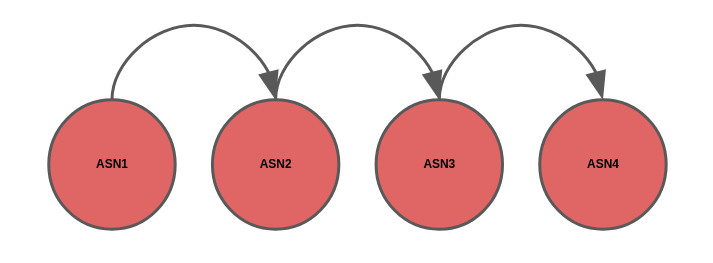
\includegraphics[width=0.5\textwidth]{img/metodologia/aspath_eejmplo_saltos.png}
    \caption{Ejemplo de camino seguido por un paquete según un AS\_PATH}
    \label{fig:aspath_eejmplo_saltos}
\end{figure}

\textbf{¿Por qué no se asume automáticamente que todas las conexiones son bidireccionales?}\\


Porque la existencia de una ruta en una dirección (por ejemplo, de ASN1 a ASN4) no garantiza que el camino inverso exista o sea utilizado. Aunque en la práctica la comunicación IP requiere que haya retorno, BGP no asegura que ese camino de vuelta sea idéntico. Para que se asuma bidireccionalidad, se debe observar también el AS\_PATH inverso explícitamente en el archivo, es decir:\\

\begin{lstlisting}[language=Python, caption=Ejemplo del camino inverso, label=code:formato_sanitized_rib_alreves]
ASN4|ASN3|ASN2|ASN1
\end{lstlisting}


La Figura~\ref{fig:aspath_ejemplos} muestra dos escenarios: (a) cuando se observa la ruta inversa, lo que indica que existe el mismo camino en sentido contrario, y (b) cómo se vería el grafo cuando se observan ambas rutas, permitiendo inferir conexión bidireccional entre los ASes.\\


\begin{figure}[h]
    \centering
    \begin{subfigure}[b]{0.45\textwidth}
        \centering
        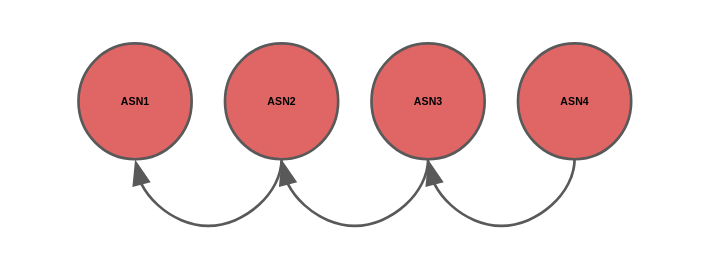
\includegraphics[width=\textwidth]{img/metodologia/aspath_eejmplo_saltos_alreves.png}
        \caption{Ruta observada en dirección inversa}
        \label{fig:aspath_eejmplo_saltos_alreves}
    \end{subfigure}
    \hfill
    \begin{subfigure}[b]{0.45\textwidth}
        \centering
        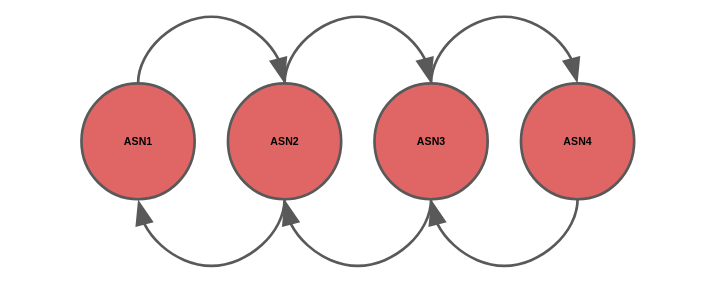
\includegraphics[width=\textwidth]{img/metodologia/aspath_eejmplo_saltos_doble.png}
        \caption{Topología resultante cuando existen ambas rutas}
        \label{fig:aspath_eejmplo_saltos_doble}
    \end{subfigure}
    \caption{Ejemplos de caminos posibles entre ASes según los AS\_PATHs observados}
    \label{fig:aspath_ejemplos}
\end{figure}

Algo importante de destacar y no confundir es que las conexiones entre ASes dadas por el AS\_PATH no están relacionadas directamente con el intercambio de mensajes BGP. La comunicación BGP entre ASes vecinos siempre es bidireccional, pero eso no implica que los AS\_PATHs observados lo sean. De otra forma, los AS\_PATHs representan rutas hacia prefijos, no las sesiones de comunicación BGP entre vecinos.

Una vez comprendida la lógica de la direccionalidad de las conexiones entre ASes dados por las RIBs, se continuó  con la construcción del grafo de Internet a partir de los datos de enrutamiento disponibles.\\

Como se mencionó previamente, en un comienzo se contaba únicamente con atributos de los ASes para la fecha 01/07/2022, extraídos del trabajo~\cite{BenchmarkingGNN}. Sin embargo, esta restricción limitaba los experimentos a una única fecha. Por esta razón, se decidió construir un conjunto de datos propios que permitiese generar atributos de los ASes para distintas fechas, según las necesidades. Sin embargo, esta tarea fue abordada más adelante en el trabajo, una vez obtenidos resultados preliminares sobre el funcionamiento de las GNNs en la tarea planteada. Esto se debió a que no era el foco principal en las primeras etapas.

Lo primero que se buscó fue encontrar una forma eficiente de almacenar la topología del grafo. Si bien, una vez obtenidas las RIBs en los archivos correspondientes, era posible construir el grafo utilizando bibliotecas como NetworkX o DGL, el proceso de leer los archivos y crear el grafo tomaba un tiempo considerable en cada ejecución. Esto se debía recorrer el archivo de las RIBs línea a línea, extrayendo cada ruta para construir de forma incremental la estructura del grafo. Adicionalmente a esto, se le debía sumar una segunda etapa, en la que se incorporaban los atributos de los nodos desde un archivo \texttt{.csv}, lo que añadía un tiempo de procesamiento adicional. Por esta razón, se buscó alguna alternativa para guardar de forma eficiente el grafo junto con sus atributos. Así se optó por utilizar el formato de almacenamiento de \textit{datasets} que ofrece DGL, el cual permite guardar la estructura del grafo con sus respectivos atributos y reutilizarlo en futuras ejecuciones de manera rápida.\\

La biblioteca DGL es una biblioteca diseñada para el fácil uso y manipulación de modelos de Redes Neuronales de Grafos (GNNs). Para guardar un grafo como dataset en el formato que propone la documentación de DGL, se crearon cuatro archivos que definen su estructura y los atributos de los nodos y aristas, según sea necesario. Estos archivos son:

\begin{itemize}
    \item Un archivo \textbf{meta.yaml} que indica qué archivo corresponde a los nodos, aristas y grafos.
    \item Un archivo \textbf{graphs.csv} que asocia un id con diferentes grafos.
    \item Un archivo \textbf{nodes.csv} con los nodos, sus atributos y el id del grafo al que pertenecen.
    \item Un archivo \textbf{edges.csv} con las aristas, sus propiedades y el id del grafo al que pertenecen.
\end{itemize}

















Un extracto del contenido de los archivos \textbf{edges.csv} (Código~\ref{code:contenido_edges}) y \textbf{nodes.csv} (Código~\ref{code:contenido_nodes}) se puede ver a continuación. En el primer caso, se incluyen cuatro columnas: la primera indica a qué grafo pertenece la adyacencia, las dos siguientes corresponden a los ASN (Autonomous System Number, por sus siglas en inglés) que representan la existencia de una relación direccional entre dos ASes, y la cuarta columna señala el tipo de relación que comparten, según el formato definido en~\ref{code:formato_out_benchmark}. En cuanto al segundo archivo, contiene tres columnas: la primera identifica el grafo al que pertenece el nodo, la segunda a un identificador del nodo (en este caso, el ASN del Sistema Autónomo) y la tercera columna almacena un string con todos los atributos asociados a dicho nodo, separados por una coma.\\


\begin{lstlisting}[language=Python, caption=Extracto contenido archivo edges.csv, label=code:contenido_edges]
graph_id,src_id,dst_id, Relationship
0,28792,6939,0
0,28792,3257,1
0,28792,9318,0
\end{lstlisting}

\begin{lstlisting}[language=Python, caption=Extracto contenido archivo nodes.csv, label=code:contenido_nodes]
graph_id,node_id,feat
0,28792,"0.2842043341251542, 0.2928342377832154, 0.3340535381175178, 0.2554473035666517, 0.0, 0.0, 1.0, 0.0, ... ,
...
\end{lstlisting}


% Explciar el codigo de crear grafo la clase q crea primero el grafo despeus agrega los attr pero esa se demora pero guaad en libreia dgl pero despues dse llama y es super rapdio ocuapr el grafo

Como se explicó previamente, leer los archivos RIBs toma tiempo, y hacerlo repetidamente no es eficiente. Por esta razón, se optó por utilizar el formato de almacenamiento descrito anteriormente (formato de \textit{datasets} de la biblioteca DGL). Sin embargo, una vez generado el archivo \texttt{sanitized\_rib.txt}, es necesario recorrerlo al menos una vez línea por línea para poder construir los tres archivos descritos (\texttt{nodes.csv}, \texttt{edges.csv} y \texttt{meta.yaml}). Para facilitar este proceso se creó una clase específica encargada de crear el grafo~\ref{code:cclase_graph}.\\

\begin{lstlisting}[language=Python, caption=Extracto clase Graph encargada de la construcción de la creación de archivos formato DGL. , label=code:cclase_graph]
class Graph:
    def __init__(self,dataset_graph_path ,max_paths,debug = False):
        self.debug = debug
        self.nx_graph = None
        self.data_path = dataset_graph_path
        
    def create_topology_from_ribs(self, rib_filename:str,filename_out="edges.csv"):
        ...
    def features_nodes(self,features_filename,filename_out="nodes.csv"):
        ...
    def remove_nodes_degree(self, degree,filename_out="edges.csv"):
        ...
...
\end{lstlisting}

\newpage
Esta clase se encarga primero de crear la topología del grafo, es decir, leer el archivo con las RIBs y generar los archivos \textbf{edges.csv} y \textbf{nodes.csv}. Una vez construida la estructura base, la clase cuenta con distintos métodos que permiten agregar atributos a los nodos según los experimentos realizados (Sección~\ref{sec:gnn_result_section}). Algunos ejemplos de atributos utilizados son métricas de centralidad como el grado del nodo, el uso del dataset mencionado previamente que ya contenía atributos para ASes en una fecha específica (detallados en la Tabla~\ref{tab:as_attr_tabla_bechmark}) , y también un conjunto de atributos generado por nosotros para otras fechas, adaptado a las necesidades del estudio (detallado en Tabla~\ref{tab:as_attr_tabla} ) .\\
 
Por último, se incluyó en el código la opción de eliminar nodos cuyo grado sea igual a un valor especificado, con el objetivo de remover nodos hoja (es decir, aquellos con grado igual a 1) que se ubican en la periferia del grafo de Internet. Esta operación puede repetirse durante una cantidad determinada de iteraciones, lo que permite simplificar la topología del grafo según los requerimientos de los distintos experimentos realizados.\\

Una vez ejecutado el bloque de código, se obtiene la siguiente estructura de carpetas y archivos, como se muestra en la Figura~\ref{repo_grap_dataset}:\\

\begin{lstlisting}[basicstyle=\ttfamily,label=repo_grap_dataset ,frame=single, caption=Estructura del repositorio del \textit{benchmark}]
dgl_graph/
    graphs.csv
    nodes.csv
    edges.csv
    meta.yaml
\end{lstlisting}

Como se mencionó en la Sección~\ref{sec:obtencion_datos_section}, en un comienzo se trabajó únicamente con los atributos de ASes extraídos del dataset utilizado en el trabajo de Giakatos et al.~\cite{BenchmarkingGNN}. Para poder utilizar esta información de manera adecuada, se desarrolló un código automatizado que permitiera identificar la fecha a la que correspondían dichos atributos. Esto se logró comparando la topología de Internet utilizada en el estudio con las topologías disponibles en el repositorio de CAIDA\cite{CAIDAS-relationship} (mismo repositorio con el que este estudio trabajó), correspondientes a diferentes fechas.\\

Para ello, se descargaron los archivos de CAIDA que contienen las conexiones entre ASes para cada mes desde 2020, considerando tanto los conjuntos serial-1 como serial-2. A partir de estos archivos, se construyó un grafo para cada fecha y se comparó su estructura con la topología utilizada en el estudio. Finalmente, se identificó la coincidencia con la topología correspondiente a julio de 2022, concluyendo que el dataset de atributos de ASes empleado en el trabajo hace referencia a esa fecha.\\

Más adelante en el trabajo, cuando se contó con un mayor conocimiento sobre los Sistemas Autónomos, así como sobre los distintos \textit{datasets} y fuentes de información pública disponibles en Internet sobre el tema, se decidió construir un conjunto propio de atributos de ASes. Esto con el objetivo de analizar y evaluar si tenían un impacto significativo en los resultados obtenidos durante los experimentos, además de evitar la limitación de fecha que se tenía para los experimentos.\\

\begin{lstlisting}[language=Python, caption=Ejemplo de mapeo de ASN a índices para entrenamiento y prueba en BGP2Vec., label=code:formato_sanitized_rib]
# ASN a índice -> x_training y x_test
x_training_mapped = []
y_training_filtered = []

# Recorrer pares (asn, asn) y agregar sólo los válidos
for (a, b), y in zip(x_training, y_training):
    a_index = asn_to_index.get(str(a), 0)
    b_index = asn_to_index.get(str(b), 0)

    # Ignorar si índice es 0 
    if a_index == 0 or b_index == 0:
        continue
    
    x_training_mapped.append([a_index, b_index])
    y_training_filtered.append(y)

# Convertir listas a arrays de NumPy
x_training_mapped = np.array(x_training_mapped)
y_training_filtered = np.array(y_training_filtered)

# ---------------------------------------------------------------------------

x_test_mapped = []
y_test_filtered = []

for (a, b), y in zip(x_test, y_test):
    a_index = asn_to_index.get(str(a), 0)
    b_index = asn_to_index.get(str(b), 0)

    # Ignorar si índice es 0 
    if a_index == 0 or b_index == 0:
        continue
    
    x_test_mapped.append([a_index, b_index])
    y_test_filtered.append(y)

x_test_mapped = np.array(x_test_mapped)
y_test_filtered = np.array(y_test_filtered)
\end{lstlisting}


\subsection{Atributos extraídos de PeeringDB} \label{sec:Atributos_extraidos_PeeringDB}

Para la obtención de atributos para los Sistemas Autónomos se utilizaron los datos de PeeringDB~\cite{PeeringDB}, un esfuerzo colaborativo donde administradores de Sistemas Autónomos aportan información sobre sus redes. Más información sobre PeeringDB puede encontrarse en el Anexo~\ref{sec:anexo_recoleccion_datos_internet}.\\

%este análisis se encuentra en el Anexo~\ref{sec:estudio_attr_peeringdb_anexo}

Para decidir los atributos más relevantes para este trabajo, primero se realizó un análisis exploratorio de los datos disponibles en PeringDB, con el objetivo de comprender el tipo de información ofrecida y su posible utilidad para la tarea de inferencia (este estudio se encuentra detallado en el Anexo~\ref{sec:anexo_exploracion_datos_peeringdb}). Luego, se llevó a cabo la preparación de los datos, que incluyó la limpieza del conjunto de datos y el tratamiento de atributos faltantes. En esta etapa, se identificaron dos tipos principales de atributos: numéricos y categóricos.\\



En el caso de los atributos categóricos, estos fueron transformados a vectores one-hot. Por otro lado, para los atributos numéricos, con el fin de homogeneizar sus rangos y reducir la variabilidad, se aplicó la función $x \rightarrow \log{(x+1)}$ y para normalizar se utilizó $x \rightarrow \frac{x - \min(x)}{\max(x) - \min(x)}$. \\

%Finalmente, para identificar las variables más relevantes para el modelo, se aplicó un proceso de selección de características....\\

% Hablar sobre pageRank

En la Tabla~\ref{tab:as_attr_tabla} se muestran los atributos que se incorporaron a los Sistemas Autónomos:\\

% TODO: Cambiar valores de los atributos numericos a como estaban antes.

\begin{table}[ht]

\centering

\footnotesize

\rowcolors{2}{grayA}{grayB}  % ← intercalado entre grisA y grisB

\begin{tabular}{|p{3.6cm}|p{6.8cm}|p{4cm}|}

\hline

\rowcolor{white}  % encabezado blanco

\textbf{Atributos} & \textbf{Descripción} & \textbf{Tipo de dato} \\

\hline

ix\_count & Cantidad de IXPs donde el AS está presente & Numérico $\in [0,1] $\\

fac\_count & Número de instalaciones donde opera & Numérico $\in [0,1]$ \\

info\_prefixes4 & Cantidad de prefijos IPv4 que anuncia la red & Numérico $\in [0,1]$ \\

info\_prefixes6 & Cantidad de prefijos IPv6 que anuncia la red & Numérico $\in [0,1]$ \\

policy\_general & Política de peering & Numérico $\in [0,1]$ \\

policy\_locations & Lugares donde aplica la política de peering & Categórico (6 categorías) \\

policy\_contracts & Requiere contrato para establecer una relación de peering& Categórico (4 categorías) \\

info\_traffic & Nivel estimado de tráfico & Categórico (19 categorías) \\

info\_scope & Alcance de la red & Categórico (11 categorías) \\

info\_type & Tipo de red & Categórico (12 categorías) \\

info\_ratio & Proporción de tráfico entrante y saliente de la red & Categórico (7 categorías) \\

PageRank & Importancia estructural del AS según su conectividad en la red & Numérico $\in[0, 6.76 \times 10^{-5}]$ \\ %ver si arreglar

\hline

\end{tabular}

\caption{Atributos considerados para representar los nodos (ASes) en la construcción del grafo.}

\label{tab:as_attr_tabla}

\end{table}


% TODO: Ver si incorporar -> Cabe destacar que para muchos ASes no se encontrba informacion, por lo que estos eran completados ? 

Con esta información se generó un archivo \texttt{.csv} que contiene los atributos de cada AS para un mes determinado, con los valores ya normalizados. Este archivo fue utilizado posteriormente al momento de construir el grafo y el dataset de la topología de Internet correspondiente a los primeros meses del año 2024.\\

%-----------------------------------------------------------------------------------------------------------------------------------------------------------------------------------------------------
\section{GNN} \label{sec:gnn_section}

Luego de creado el dataset correspondiente al grafo de Internet, se comenzó a abordar la tarea de inferencia utilizando Redes Neuronales de Grafos (GNN), donde se adoptaron dos enfoques:

\begin{enumerate}

    \item \textbf{Entrenamiento por etapas}: En este enfoque, el pipeline se divide en dos etapas. La primera, donde se aprenden las representaciones de los nodos (embeddings) utilizando GNNs. Y la segunda, donde estas representaciones se utilizan como entrada para una Red Neuronal Artificial (ANN), que actúa como clasificador para realizar la tarea de inferencia.
    
    \item \textbf{Entrenamiento end-to-end}: En este segundo enfoque, el modelo GNN aprende las representaciones de los nodos —es decir, se entrena— con base en la tarea específica, en este caso, la clasificación de aristas.  
    
    % puede causar overfitting?
    

\end{enumerate}

En ambos enfoques se tomó un esquema encoder-decoder, donde la GNN actúa como codificador (\textit{encoder}), generando representaciones vectoriales para cada nodo, las que son luego utilizadas por un decodificador (\textit{decoder}), cuya implementación varía según la tarea y el enfoque utilizado. \\

Las arquitecturas de GNNs que se utilizaron fueron: GCN (Graph Convolutional Network), GraphSAGE (SAmple and aggreGatE) y GAT (Graph Attention Network). Como \textit{decoder}, se utilizó una MLP (Multilayer Perceptron) en ambos enfoques. También, en el enfoque por etapas se ocupó un decodificador basado en producto punto (Dot Product) para la tarea de predicción de enlaces, mientras que en el enfoque end-to-end se consideró también un decodificador Bilinear para la clasificación de relaciones.\\ 
%(Más información sobre los decoders utilizados en ANEXO\ref{anexo:decoders}).\\




En el Codigo~\ref{code:modelo_gcn} correspondiente a una clase que implementa un modelo basado en GCN. En este ejemplo, el método \textit{encode} realiza el forward pass, correspondiente a las dos capas GNN, mientras que los métodos \textit{decodeDotProduct}, \textit{decodeMLP} y \textit{decodeBilinear} actúan como \textit{decoders}.\\

\begin{lstlisting}[language=Python, caption=Ejemplo modelo GraphSAGE , label=code:modelo_gcn]
class GCN(nn.Module):
    def __init__(self, in_feats, hidden_feats, out_feats, out_feats_mlp=1, drop=0.3):
        super().__init__()
        self.conv1 = GraphConv(in_feats, hidden_feats)
        self.conv2 = GraphConv(hidden_feats, out_feats)
    
        self.MLP = MLPPredictor(out_feats,out_feats_mlp)
        self.BilinearDecoder = BilinearPredictor(out_feats, 3)
        self.regressor = nn.Linear(out_feats, 1)
        self.drop  = nn.Dropout(drop)           


    def encode(self, g, x):
        g = dgl.add_self_loop(g)
        h = self.drop(F.relu(self.conv1(g, x)))  
        h = self.conv2(g, h)                     
        return h

    
    def decodeDotProduct(self, g, h):
        with g.local_scope():
            g.ndata["h"] = h
            # Compute a new edge feature named 'score' by a dot-product between the
            # source node feature 'h' and destination node feature 'h'.
            g.apply_edges(fn.u_dot_v("h", "h", "score"))
            # u_dot_v returns a 1-element vector for each edge so you need to squeeze it.
            return g.edata["score"][:, 0]
        
    def decodeMLP(self, g, h):
        return self.MLP(g, h)  
    
    def decodeBilinear(self, g, h):
        return self.BilinearDecoder(g, h)

    def forward(self, g, x):
        h = self.encode(g, x)  # Embeddings
        out = self.regressor(h).squeeze(-1)  # Predicción final
        return out 
        
\end{lstlisting}

Cabe mencionar que en el entrenamiento en Redes Neuronales de Grafos existen diferentes modalidades para entrenar un modelo, dependiendo de cómo se utilicen los nodos y el grafo durante el entrenamiento e inferencia.\\


%existen diferentes modalidades para entrenar un modelo, en primera instancia en cómo se utilizan los nodos y el grafo durante el entrenamiento e inferencia:\\

\begin{itemize}
    \item \textbf{Inductivo:} El conjunto de entrenamiento y el de prueba están completamente separados, es decir, se trabaja con grafos distintos. Este enfoque permite una mejor generalización, ya que el modelo debe generar predicciones sobre nodos y estructuras que no ha visto antes. Sin embargo, una desventaja es que no siempre se cuenta con múltiples grafos para poder entrenar y evaluar el modelo.
    
    \item \textbf{Transductivo:} Se tiene un único grafo que se usa tanto para el entrenamiento como para la inferencia. Sin embargo, la función de pérdida se calcula solamente sobre los nodos que se definieron como parte del conjunto de entrenamiento. Este enfoque es útil cuando se cuenta con un único grafo completo y se debe predecir información específica dentro del mismo.\\
    
\end{itemize}

Para trabajar con estos enfoques y nuestros datos, la separación del grafo en entrenamiento y test se trabajó de la siguiente forma:

\begin{itemize}

    \item \textbf{Usar el grafo completo con pérdida filtrada (enfoque transductivo):} \\
    En este caso se utiliza el grafo completo durante el entrenamiento, pero la función de pérdida se calcula solo sobre los elementos del conjunto de entrenamiento (ya sean nodos o aristas).
    Se aplicó en dos casos:
    \begin{itemize}
        \item \textbf{Clasificación de aristas} (en el enfoque end-to-end)
        \item \textbf{Predicción de atributos de nodos} (en el enfoque por etapas para la generación de embeddings)
    \end{itemize}
    
    \item \textbf{Crear subgrafos separados (enfoque inductivo):} \\
    Se generan dos subgrafos separados a partir del grafo principal, uno para el entrenamiento y otro para la validación, eliminando las aristas correspondientes.\\
    Se aplicó en el caso:
    \begin{itemize}
        \item \textbf{Predicción de aristas} (en el enfoque por etapas). Evita que el modelo tenga acceso a las aristas que luego debe predecir, reduciendo el riesgo de fuga de información.
    \end{itemize}
\end{itemize}


% \usepackage{booktabs}
% \usepackage{tabularx}


% Paquetes recomendados en el preámbulo:
% \usepackage{array,longtable,booktabs,enumitem}
% Definir un tipo de columna alineada a la izquierda con ancho fijo:
\newcolumntype{P}[1]{>{\raggedright\arraybackslash}p{#1}}

\begin{longtable}{P{0.27\textwidth} P{0.45\textwidth} P{0.24\textwidth}}
\caption{Estrategias de entrenamiento de los datos según la tarea con GNN.}
\label{tab:division_grafo_estrategias_long} \\
\toprule
\textbf{Estrategia} & \textbf{Descripción} & \textbf{Se aplicó en} \\
\midrule
\endfirsthead
\toprule
\textbf{Estrategia} & \textbf{Descripción} & \textbf{Se aplicó en} \\
\midrule
\endhead

Grafo completo con pérdida filtrada
&
Se usa el grafo completo durante el entrenamiento, pero la función de pérdida se calcula \emph{solo} sobre los elementos del conjunto de entrenamiento (nodos o aristas).
&
\begin{itemize}[leftmargin=*,nosep]
  \item Clasificación de aristas (enfoque end-to-end).
  \item Predicción de atributos de nodos (enfoque por etapas para generar \textit{embeddings}).
\end{itemize}
\\
\addlinespace
Subgrafos separados (train/valid)
&
Se generan dos subgrafos disjuntos (entrenamiento y validación) eliminando las aristas correspondientes. Evita que el modelo acceda a aristas que luego debe predecir, reduciendo la fuga de información.
&
Predicción de aristas (enfoque por etapas).
\\
\bottomrule
\end{longtable}


%Otro aspecto adicional fue que para evitar fuga de información, incluir ambas aristas dirigidas de un mismo par de nodos dentro de el mismo conjunto de entrenamiento o validación.\\


Una vez definidos los conjuntos de entrenamiento y validación, se procedió al entrenamiento de los modelos. Para ello, se trabajó con \textit{early stopping} para evitar sobreajuste. Además, se monitorearon métricas como la pérdida y la Accuracy a lo largo de los epochs, y se evaluó el rendimiento final mediante el uso de matrices de confusión y las métricas de evaluación. 































%/////////////////////////////////////////////////////////////////////
% SEGUNDO ENFOQUE: EMB+TASK--------------------------------------

\subsection{Primer Enfoque: \textit{Por etapas} }



Como se mencionó anteriormente, se trabajó con dos enfoques de flujo de entrenamiento. 
El primero, denominado \textit{por etapas}, es más útil cuando se dispone de un conjunto de datos de etiquetado limitado o para generar representaciones que luego serán utilizadas para diferentes tareas (\textit{downstream task}). 
En este esquema hay dos etapas: primero, se aprenden las representaciones de los nodos. Luego, estas representaciones son utilizadas como entrada a una ANN que actúa como clasificador. Para este caso se suele tener un rendimiento inferior en comparación con el enfoque \textit{end-to.end}, sin embargo, al ser las representaciones más genéricas, pueden utilizarse para múltiples tareas.\\


En la Figura~\ref{fig:diagrama-de-flujo-efoque2} se muestra el flujo general de este enfoque. La entrada consiste en las rutas BGP previamente sanitizadas (\texttt{sanitized\_ribs.txt}), a partir de las cuales se construye la topología del grafo de Internet. Luego, una GNN genera embeddings a partir de la información estructural y de atributos de los nodos —la selección de estos atributos se detalla más adelante—. Estas representaciones son luego utilizadas como entrada para una ANN, encargada de inferir la relación entre pares de nodos.\\

\begin{figure}[h]
    \centering
    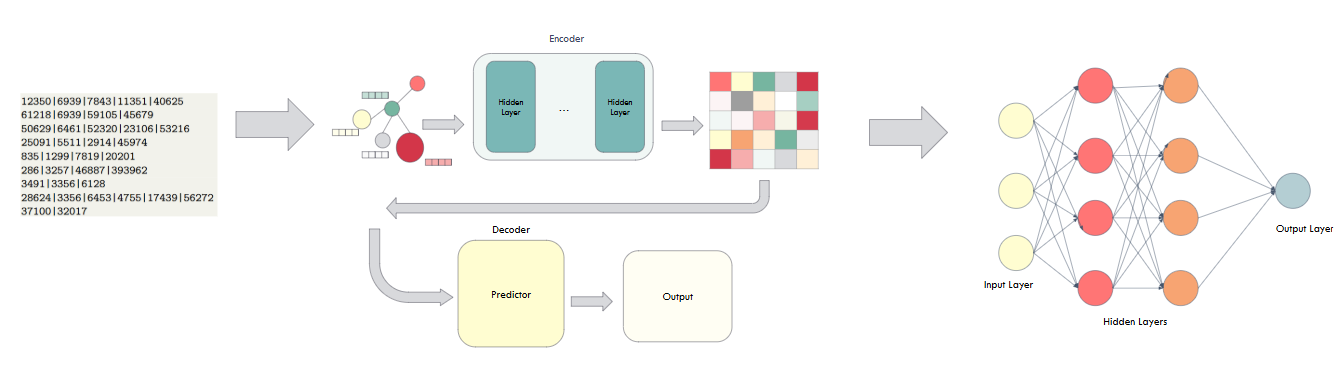
\includegraphics[width=1\textwidth]{img/gnn/gnn-enfoque-2.png}
    \caption{Diagrama de flujo del primer enfoque: Entrenamiento de embeddings de nodos para luego pasar la entrada a una ANN para la tarea de clasificación}
    \label{fig:diagrama-de-flujo-efoque2}
\end{figure}

%TODO: Agregar en inform eq esto se agregó
\begin{algorithm}[H]
\caption{Entrenamiento por etapas para inferencia de relaciones entre ASes}
\label{alg:gnn_por_etapas}
\begin{algorithmic}[1]
\Require Grafo $G$, atributos de nodos $X$, tarea auxiliar $T$, pares etiquetados $(u,v,y)$
\Ensure Clasificador entrenado para inferencia de relaciones
\State Inicializar encoder GNN
\State Entrenar la GNN sobre la tarea auxiliar $T$
\State Obtener embeddings de nodos $H$
\State Construir vectores de entrada para pares $(u,v)$ a partir de $H$
\State Entrenar un clasificador supervisado sobre las etiquetas $y$
\State Evaluar el clasificador sobre el conjunto de prueba
\end{algorithmic}
\end{algorithm}

El flujo general del enfoque por etapas se resume en el Algoritmo~\ref{alg:gnn_por_etapas}.





Las tareas utilizadas para crear las representaciones vectoriales de los Sistemas Autónomos en el grafo de Internet fueron:\\

\begin{enumerate}

    \item \textbf{Predicción de existencia de arista entre nodos}: Se trabajó sobre una tarea binaria, donde se entrenó al modelo para distinguir si dos pares de nodos estaban conectados o no (generando aristas negativas). Esto permite que los embeddings capturen patrones de conectividad entre los nodos.

    \item \textbf{Predicción de atributos}: El modelo se entrena para predecir propiedades específicas de los nodos, en este caso, su \textit{grado} y su valor de \textit{PageRank}. El objetivo de esto es hacer que la GNN aprenda representaciones que reflejen la posición y el rol estructural de cada nodo dentro del grafo.

\end{enumerate}




Para la segunda etapa correspondiente a la predicción de relaciones, se utilizó una Red Neuronal que recibe como entrada los embeddings de dos nodos adyacentes. Esta red combina la información de ambos nodos y retorna una predicción sobre el tipo de relación existente entre ellos. Sin embargo, antes de trabajar directamente con los datos de entrenamiento y evaluación, fue necesario adaptarlos para que pudieran ser utilizados junto a los embeddings generados previamente por la GNN. Para esto, se creó un diccionario que asignaba un ID a cada ASN, de forma que los embeddings pudieran ser asociados de manera consistente. Los IDs fueron definidos en base al valor de los ASN, para de esta forma facilitar la interpretación de los resultados y mantener una trazabilidad más simple.\\



Dado que los modelos de embeddings trabajan con IDs en lugar de valores simbólicos como los ASN (forma en que nuestro dataset ToR era identificado), se tuvo que adaptar el conjunto de entrenamiento y prueba. Específicamente, se mapeó cada ASN a un ID utilizando un diccionario que se creó previamente en el trabajo, si alguno de los ASN no era encontrado en dicho diccionario (es decir, no tenía un ID asociado), el nodo era descartado del conjunto (Código~\ref{code:mapeo_asn_id}).\\



%, si alguno de los ASN no se encontraba en los conjuntos, no se encontraba presente en el diccionario (es decir, no tenía un ID asociado); este ejemplo se descartaba del conjunto (Código~\ref{code:mapeo_asn_id}). \\



\begin{lstlisting}[language=Python, basicstyle=\ttfamily\footnotesize, label=code:mapeo_asn_id, frame=single, caption={Modelo CNN utilizado en el enfoque BGP2VEC para clasificación de relaciones AS.}]
# Mapeo de ASN a índices para conjuntos de entrenamiento
x_training_mapped = []
y_training_filtered = []

# Recorrer cada par (asn, asn) en entrenamiento y filtrar válidos
for (a, b), y in zip(x_training, y_training):
    a_index = asn_to_index.get(str(a), 0)
    b_index = asn_to_index.get(str(b), 0)

    # Ignorar si alguno de los índices es 0 (no mapeado)
    if a_index == 0 or b_index == 0:
        continue

    x_training_mapped.append([a_index, b_index])
    y_training_filtered.append(y)

# Convertir a arreglos NumPy
x_training_mapped = np.array(x_training_mapped)
y_training_filtered = np.array(y_training_filtered)

# ---------------------------------------------------------------------------
# Mismo proceso para el conjunto de prueba
x_test_mapped = []
y_test_filtered = []

for (a, b), y in zip(x_test, y_test):
    a_index = asn_to_index.get(str(a), 0)
    b_index = asn_to_index.get(str(b), 0)

    if a_index == 0 or b_index == 0:
        continue

    x_test_mapped.append([a_index, b_index])
    y_test_filtered.append(y)

x_test_mapped = np.array(x_test_mapped)
y_test_filtered = np.array(y_test_filtered)

# Guardar los datos procesados
np.save(PATH + DATA + "x_training_mapped.npy", x_training_mapped)
np.save(PATH + DATA + "y_training_filtered.npy", y_training_filtered)
np.save(PATH + DATA + "x_test_mapped.npy", x_test_mapped)
np.save(PATH + DATA + "y_test_filtered.npy", y_test_filtered)
\end{lstlisting}




La Red Neuronal utilizada en esta etapa fue la misma propuesta en el enfoque BGP2Vec para la clasificación de relaciones entre Sistemas Autónomos. Este modelo se basa en una arquitectura de \textit{Convolutional Neural Network (CNN)}. La entrada corresponde a secuencias de pares de identificadores, correspondientes a los ASN involucrados. Estos IDs son transformados en sus representaciones vectoriales mediante una capa de tipo \textit{Embedding}, la cual puede estar fija (no entrenable) o entrenarse junto al modelo, dependiendo del experimento. Luego, se aplican capas convolucionales para extraer patrones espaciales en las representaciones, seguidas por capas de \textit{MaxPooling}, \textit{Flatten} y, finalmente, capas densas que concluyen en una función \textit{softmax} para obtener una salida única que corresponde a la clase predicha.\\

\newpage
A continuación se muestra el código correspondiente a la implementación del modelo:\\





\begin{lstlisting}[basicstyle=\ttfamily, label=code:cnn_bgp2vec_model, frame=single, caption=Modelo CNN utilizado en el enfoque BGP2VEC para clasificación de relaciones AS.]
# Configuración de la red BGP2VEC
experiment = None
num_classes = len(class_names)
embedding_trainable = False
input_length = 2  # Longitud de la secuencia de entrada
embedding_vector_length = embeddings.shape[1]  # Dimensión de los vectores de embedding
total_ASNs = embeddings.shape[0]  # Tamaño del vocabulario (número de ASes)

# Definición del modelo
model = Sequential()
model.add(Embedding(total_ASNs, embedding_vector_length, input_length=input_length,
                    weights=[embeddings], trainable=embedding_trainable))
model.add(Conv1D(filters=32, kernel_size=3, padding='same', activation='relu'))

model.add(Reshape((32, 2)))  # Ajuste necesario de dimensiones para la siguiente capa
model.add(MaxPooling1D(pool_size=2))

model.add(Conv1D(filters=32, kernel_size=3, padding='same', activation='relu'))
model.add(Reshape((32, 16)))  # Nuevo ajuste de dimensiones
model.add(MaxPooling1D(pool_size=2))

model.add(Flatten())
model.add(Dense(100, activation='relu'))
model.add(Dense(num_classes, activation='softmax'))
\end{lstlisting}

Una breve explicación de las demás capas utilizadas en esta arquitectura, además de las convoluciones:\\

\begin{itemize}

    \item \textbf{MaxPooling1D:} Reduce la dimensión de la salida de una capa convolucional tomando el máximo valor dentro de una ventana deslizante sobre la secuencia de datos.

    \item \textbf{Flatten:} Toma una entrada multidimensional (por ejemplo, una matriz o un tensor 3D) y la aplana en un vector 1D. Convierte la salida de las capas convolucionales y de pooling en un formato que pueda ser usado por las capas densas (Dense).

    \item \textbf{Dense:} Es una capa completamente conectada (fully connected), donde cada neurona está conectada a todas las salidas de la capa anterior.

    \item \textbf{Función softmax:} Convierte el vector de valores reales (logits) en un vector de probabilidades, donde cada valor queda entre 0 y 1 y la suma de ellos es 1.\\

\end{itemize}

Un problema que se conocía desde el inicio, y que se hizo especialmente evidente a partir de los primeros resultados del modelo, fue el del desbalance de clases presente en el dataset. Este se evidencia en la Figura~\ref{fig:relaciones_por_tipo_asrank} donde se observa que hay una cantidad considerablemente mayor de relaciones P2P que de C2P.\\

%Esto también se aprecia en los resultados obtenidos, como se muestra en las Figuras ~\ref{fig:anex:matrices_confusion_experimentos_gnns_decoder}  correspondientes a las matrices de confusión para diferentes experimentos.\\

Para trabajar este problema, se calcularon pesos específicos para cada clase en función de su frecuencia en el conjunto de entrenamiento. Con estos valores se crea un diccionario \texttt{class\_weight\_dict}, el cual se utiliza para ajustar la función de pérdida para las diferentes clases, asignando mayor peso a las clases menos representadas y menor peso a las clases más frecuentes (Código~\ref{code:class_weights_dict}).\\

\begin{lstlisting}[basicstyle=\ttfamily, label=code:class_weights_dict, frame=single, caption=Estructura del repositorio de los experimentos para la tarea de inferencia usando GNNs]
from sklearn.utils import class_weight
import numpy as np

class_weights = class_weight.compute_class_weight(
                    class_weight='balanced', 
                    classes=np.array(list(range(num_classes))), 
                    y=y_training_filtered)

class_weight_dict = {i: w for i, w in enumerate(class_weights)}
# {0: 0.49730749665083795, 1: 2.020894588161655, 2: 2.0228938408395782}
print('[class_weights_dict]:', class_weight_dict)
\end{lstlisting}

También se decidió generar representaciones vectoriales (embeddings) de los nodos utilizando el algoritmo \textbf{DeepWalk}, para comparar su desempeño respecto a los embeddings generados por la GNN. A diferencia de las GNN, DeepWalk se basa únicamente en la estructura del grafo.\\




%/////////////////////////////////////////////////////////////////////
%/////////////////////////////////////////////////////////////////////
% Segundo ENFOQUE: END-TO-END --------------------------------
\subsection{Segundo Enfoque: \textit{end-to-end} }
\label{sec:SegundoEnfoque}
Este enfoque (\textit{end-to-end}) es útil cuando se tiene un conjunto suficiente de datos etiquetados, ya que permite que la GNN aprenda representaciones directamente de la tarea de clasificación. Esto hace que las representaciones aprendidas sean muy específicas, por lo que no siempre pueden reutilizarse en otros contextos.\\

% TODO:Agregar mas citas de donde saco las cosas y a que esepcificamente me refiero

% TODO: Comentar como se hizo el split?
En la Figura~\ref{fig:diagrama-de-flujo-endtoend1}, se observa el flujo de entrenamiento. Como entrada, se entrega el grafo con los respectivos atributos de los nodos y las etiquetas de las relaciones (aristas). El encoder corresponde a arquitecturas GNN, las cuales generan embeddings para cada nodo. Estas representaciones son utilizadas por alguno de los decoders, produciendo así un vector de puntuaciones para cada posible relación. La clase con mayor puntaje es seleccionada como predicción. A partir de este resultado se calcula la función de pérdida, la cual, mediante el backpropagation, ajusta de forma conjunta tanto los parámetros del encoder como del decoder.\\

\begin{figure}[h]

    \centering

    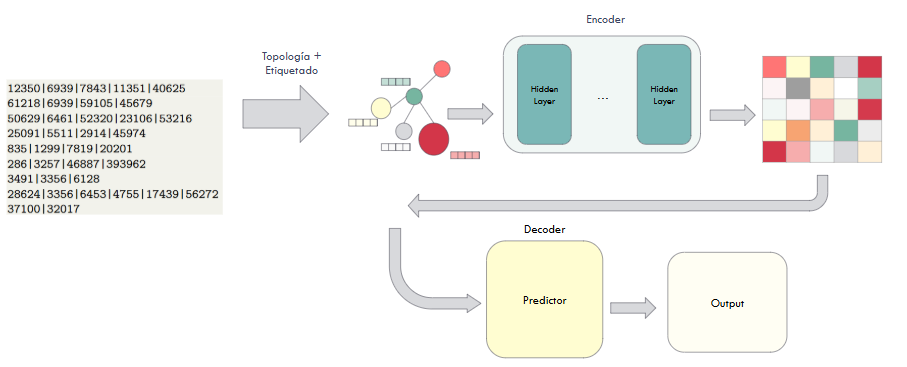
\includegraphics[width=0.9\textwidth]{img/gnn/gnn-endtoend1.png}

    \caption{Diagrama de flujo del entrenamiento \textit{end-to-end}.}

    \label{fig:diagrama-de-flujo-endtoend1}

\end{figure}





%TODO: se agrgo aqui esto infome
\begin{algorithm}[H]
\caption{Entrenamiento end-to-end para clasificación de relaciones entre ASes}
\label{alg:gnn_end_to_end}
\begin{algorithmic}[1]
\Require Grafo $G$, atributos de nodos $X$, aristas etiquetadas $E_L$
\Ensure Modelo encoder-decoder entrenado
\State Inicializar encoder GNN y decoder
\For{cada época}
    \State Generar embeddings de nodos a partir de $G$ y $X$
    \State Predecir etiquetas sobre las aristas de entrenamiento
    \State Calcular la función de pérdida
    \State Actualizar parámetros mediante backpropagation
\EndFor
\State Evaluar el modelo sobre las aristas de validación o prueba
\end{algorithmic}
\end{algorithm}

El flujo general del enfoque end-to-end se resume en el Algoritmo~\ref{alg:gnn_end_to_end}.






Como se mencionó anteriormente, en esta tarea se utilizó el grafo completo para el entrenamiento, pero filtrando las aristas al momento de calcular la función de pérdida, de modo que solo se consideraran aquellas que pertenecían al conjunto de entrenamiento.

En este enfoque, luego de cargar el grafo, se procedió a etiquetar las aristas utilizando el dataset de relaciones provisto por CAIDA. Debido a la baja cantidad de ejemplos disponibles para ciertos tipos de relaciones, se decidió incorporar todas las aristas que se encontraban presentes en el conjunto de datos de CAIDA. Esta decisión permitió ampliar la cantidad de muestras etiquetadas y así facilitar el entrenamiento del modelo en la tarea de clasificación de aristas.\\

Durante esta etapa se realizaron distintas variaciones de experimentos con el objetivo de evaluar el impacto de las decisiones de diseño del modelo. Se probaron diferentes arquitecturas de GNN, combinadas con distintos tipos de decodificadores. Además, se evaluaron distintos esquemas de atributos de nodos: atributos reales sacados de PeeringDB, atributos basados únicamente en el grado de los nodos, y atributos aleatorios.\\

Además, se exploró el uso de técnicas de \textit{sampling}, en particular \texttt{Neighbor Sampling}, donde para cada batch se toma un subconjunto de nodos y un número fijo de vecinos por capa, y \texttt{ClusterGCN}, que agrupa el grafo en pequeños subgrafos (clusters) y entrena sobre ellos por separado.
Se probaron estas técnicas para observar cómo cambia el resultado al entrenar con menos información de la estructura del grafo.\\





.







\subsection{Distribución del Repositorio}

Al igual que en el \textit{benchmark} mencionado previamente (Sección~\ref{sec:Benchmark_section}), en este caso también se utilizó un repositorio distinto en GitHub~\cite{gnnCode} para trabajar y almacenar el código, además de servir como sistema de control de versiones. Permitiendo así trabajar desde diferentes dispositivos.\\


La Figura~\ref{benchmark_repo_estructura} muestra la estructura del repositorio que se utilizó para los experimentos utilizando GNNs. El directorio contiene los datos, los resultados, los módulos implementados y diversos notebooks con los diferentes enfoques que se utilizaron.\\

\begin{lstlisting}[basicstyle=\ttfamily, label=benchmark_repo_estructura, frame=single, caption=Estructura del repositorio de los experimentos para la tarea de inferencia usando GNNs.]
data/
results/
modules/
    gnn_models.py
    gnn.py
    graph.py
AS_relationship_inference_gnn.ipynb
train_embeddings.ipynb
AS_relationship_inference.ipynb
create_as_attr.ipynb
create_graph.ipynb
utils.py
\end{lstlisting}

Dentro del directorio \texttt{data/} se almacenan todos los archivos necesarios para la realización de los experimentos: los embeddings de los Sistemas Autónomos generados durante el entrenamiento, los modelos entrenados, los archivos necesarios para la construcción del grafo de ASes, así como las RIBs ya sanitizadas, los \textit{datasets} con las relaciones entre ASes extraídas de CAIDA y los archivos provenientes de PeeringDB.\\

Por otro lado, el directorio \texttt{results/} almacena los resultados de todos los experimentos realizados. Estos se guardan en archivos \texttt{.csv} con el formato mostrado en la Figura~\ref{code:formato_out_benchmark}. Además, en esta carpeta se encuentran los gráficos generados a partir de dichos resultados.\\


La carpeta \texttt{modules/} contiene tres archivos \texttt{.py}, cada uno con una clase que agrupa funcionalidades específicas utilizadas durante el flujo de los experimentos:
\begin{itemize}
    \item \texttt{gnn.py}: agrupa las funciones necesarias para la ejecución del pipeline de entrenamiento con GNNs.
    \item \texttt{graph.py}: contiene la clase responsable de construir el grafo a partir de las RIBs y otros archivos, adaptándolo al formato utilizado en este proyecto.
    \item \texttt{gnn\_models.py}: define las distintas arquitecturas de modelos GNN utilizadas en los experimentos.
\end{itemize}



Los notebooks \texttt{AS\allowbreak\_relationship\allowbreak\_inference\allowbreak\_gnn.ipynb}, \texttt{train\allowbreak\_embeddings.ipynb} y \texttt{AS\allowbreak\_relationship\allowbreak\_inference.ipynb} corresponden al flujo de trabajo de los dos enfoques de inferencia: \textit{end-to-end} y por etapas, respectivamente.

Finalmente, el archivo \texttt{create\_as\_attr.ipynb} se encarga de descargar y generar un archivo \texttt{.csv} con los atributos asociados a los ASes para una fecha determinada\\


% \subsection{Creación Dataset} \label{sec:metodologia_creacion_dataset}

% Con el objetivo de dejar disponible un conjunto de datos sobre Internet para usos más generales, se creó un dataset en el formato previamente explicado de la biblioteca DGL (Deep Graph Library). Este dataset está compuesto por un conjunto de grafos que representan la topología de Internet a nivel de Sistemas Autónomos (AS) para cada mes del año 2024. En cada grafo, los nodos corresponden a ASes y contienen como atributos información extraída de PeeringDB como se explico en la Sección~\ref{sec:Atributos_extraidos_PeeringDB}.


% A diferencia del dataset construido anteriormente —el cual contiene un único grafo con el que se trabaja—, este nuevo conjunto incluye múltiples grafos, uno por cada mes. Sin embargo, la estructura de carpetas y archivos donde se almacena la información sigue el mismo esquema mostrado en el Código~\ref{repo_grap_dataset}. La principal diferencia se encuentra en que los archivos de este nuevo dataset incorporan un header adicional, \texttt{graph\_id}, que permite distinguir los nodos y las aristas pertenecientes a cada uno de los grafos.



% \begin{lstlisting}[language=Python, caption= Como se ve el archivo nodes.csv, label=archivo_nodes_todos_meses]


% graph_id,node_id,feat
% 0,0,"0.5725330322207948,0.8451870383322376,0.44412796119211184"
% 0,1,"0.6624186423087752,0.6118386331195641,0.7352138669985214"
% 0,2,"0.7583372765843964,0.15218126307872892,0.6810484348765842"
% ...


% \end{lstlisting}


% \begin{lstlisting}[language=Python, caption=Cómo se ve el archivo edges.csv, label=archivo_edges_todos_meses]
% graph_id,src_id,dst_id,feat
% 0,0,4,"0.39534097273254654,0.9422093637539785,0.634899790318452"
% 0,3,0,"0.04486384200747007,0.6453746567017163,0.8757520744192612"
% ...
% \end{lstlisting}



% \subsection{COSAS A AGREGAR QUE SE ME VAN OCURRIENDO (no se si incluir)}



% \textbf{PAREJAS (u,v) VS (v,u)
% }Un problema que se penso a medio camino fue los pares de nodos $(u,v)$ vs $(v,u)$ al momento de entrenar los modelos GNN, especificamente fue un problema en el split del las aristas. Especificamente al momento de mandar la arista (u,v) a train y (v,u) a test, filtrando información del mismo vínculo. Para resolver este problema se tiene agrupa los pares o trabaja con grafos sin duplicar direcciones para evitar data leakage.
% 	Las dos direcciones nunca quedan en splits distintos.\\

% \textbf{OTRAS COSAS DEL SPLIT
% }train\_g se construye eliminando TODAS las aristas de val/test.
% Nos preguntamos, tenemos dos enfoques para crear el split del dataset cuando se trata de hacer split de aristas. 
% - El primero donde el grafo con el que se entrena el modelo, se le eliminan las aristas que se encuentran en le conjunto de validacion
% - El segundo donde no las elimino, pero solo incluyo en el calculo de la loss, aquellas aristas que se encuentran en el conjuntos de entrenamiento.

% \textbf{ARISTAS SIN ETIQUETA (enfoque endt/to/end)
% }En caso de entrenamiento end-to-end al teenr unicamente las etiquetas dadas por el dataest de CAIDA AS Relationships, sucedia que existian alguans aristas del nodo construido a aprtir de las RIBs que quedaban sin etiqueta. Teniamos 3 posibles caminos:
% - Dejas la arista en el grafo de mensajes para no aislar nodos, pero al momento de calcula la loss no se incluian.
% - Asignas etiqueta 3 a los enlaces sin etiqueta y entrenar un clasificador de 4 clases.
% - Aplicar uno de los método previos (Gao, Ruan, ProbLink, etc.) sobre los enlaces sin etiqueta y los tomarlo como pseudo-label.
% Se tomo el primer enfoque.

% Como teniamos mas relaciones , que etiquetas, las aristas que no tenian etiquetas las etiquetamos como el valor -1 (para no hacerlas desaparecer y asi sigan dentro de train\_g, con lo que participan en el message-passing y aportan contexto topológico a los otros nodos. Lo único que hacemos es excluirlas del cálculo de la pérdida y de las métricas (porque no sabemos si son P2P, C2P o P2C). [Solo alimentamos los logits/labels cuyas etiquetas son 0, 1 o 2]


% \textbf{EARLY STOPPING Y VALIDACIO}
% Otra cosa que se realizo mas adelante, una ves ya construidos los modelos y tenido una base mínima fue realizar \textit{Early-stopping} y \textit{validación}. Para esto se modifico el metodo encargado de el pslit del dataset y detener el entrenamiento del modelo una ves la pérdida del conjunto de validacion deje de mejorar, de esta forma se evita sobre-entrenar a ciegas y evitar un posible overfiting.\\

% \textbf{AGREGAR UNA CAPA DE DROPUT/REGULARIZACION}
% Dos capas + ReLU a menudo basta; añade nn.Dropout(0.3) entre capas del encoder y del MLP para reducir sobre-ajuste.


% \textbf{COMPROBAR COINCIDENCIAS MI GRAFO CON CAIDA}
% En algun moemnto cosas no funcionan. Una de esas cosaspara comprobar que todo estubiese bien compare cuantas aristas coincidian CAIDA AS Relationships y el graf oque cree a partir de las RIBs.
% Coinciden 18 de 142979 aristas del grafo (0.01%)
% Coinciden 18 de 488777 aristas del archivo CAIDA (0.00%)


% \textbf{AJUSTES MODELOS PARA LOS DOS ENFOQUES
% }por ejemplo sabemos que para este caso es mejor no hacer q con mlp salga solo un valor porq en egenral s edan malas salida, por eso la idea es q la salida sea 3 y luego aplicarg argmax. y desntro de la mis meodo esto s epuede hacer par ano repetir ocidgp MLPPredictor(8,3)
% \usepackage{adjustbox}





% Un porblma que dinos cuenta mas adelante fue que por jemplo en los resultados del enfoque por parte la mayoria de los resultados iban se amontonaban o iba  ainferencias del tipo p2p. En un principio se asumio que se debia a que en el ataset segundo de relacioens la mayoria correspondia a relaciones del tipo p2p, cais el doble de los otros dos tipo. Sin embargo al moemnto de empezar el segundo enfoque nos dimso cuenta que el problema estaba que al ocupar solo 1.000.000 de path de los RIBs, estas en su  mayoria eran P@P, loq ue significaba que al entrenar embeddings en su mayoria entrenamso embeddings p2p y por tanto saber como hacer represnetaciones de estos pero no muy bien de las otras.
% De hehco si  para el enfoque por parte entreneabmso los embeddings en base al grafo creado a partir de CAI pero sirve como para saber como seria un caso no overfiteado en p2p.DA (esto no tiene sentido hacerlo para la tarea especifica de nosotros)


% Otro problema que tuvimos fue l que, como vimos al sacar solo 1.000.000 de paths de las RIBs la mayoria de las relaciones xistentes n estas son P2P. Entonces al momento de centrarnos en el segundo enfoque donde tenemos directamente que prdecir las relaciones que sacamos de las RIBs, stas son insuficientes. 
% Por que esto no sucede con el enfoque de por partes? sto porqu eal final las relaciones que predecimos son directamente todas las del dataset de CAIDA AS Relationships. Pero en este caso (por partes) sucede que ocupamos el mismo datast (la misma particion test/train) pero como no obtenmos tooooodas las relacions del grafo porq solo sacamos 1.000.000 PATHS , no logramos compltar edsas relaciones en l grafo y por tanto se liiminan, qudandonos asi con una muy pequña parte de relaciones P2C y C2P.

% Ahi es cuando se mpzo a optimmizar el codigo para crear el datast con todos los AS PATHS y se logro. Pero luego al corrr en l pc la funcion de la librria para leer el grafo moria. 
% Siqu se corrio en colab.






\chapter{Resultados}

A continuación, se muestran los resultados obtenidos de los distintos experimentos realizados, tanto en la evaluación del uso de Redes Neuronales de Grafos para la tarea (Sección~\ref{sec:gnn_result_section}) como en el \textit{benchmark} de métodos de inferencia de relaciones entre ASes (Sección~\ref{sec:benchmark_result_section}). Además, se incluye una exploración de las RIBs extraídas y del dataset de evaluación ocupado (Sección~\ref{sec:analisis_datasets_section}).\\


%/////////////////////////////////////////////////

\section{Análisis y caracterización de los datos} \label{sec:analisis_datasets_section}

Como se indicó previamente, para este trabajo se utilizaron diferentes conjuntos de datos. En primer lugar, se emplearon las RIBs extraídas desde recolectores BGP, a partir de las cuales se obtuvo la topología de Internet y, por ende, las conexiones existentes entre Sistemas Autónomos. Además, se utilizó el conjunto de datos de CAIDA AS Relationships, el cual fue usado para evaluar los modelos del \textit{benchmark} y entrenar la Red Neuronal de Grafos (GNN). Este conjunto consiste en un archivo que etiqueta relaciones entre ASes, generadas por el método del estado del arte AS Rank~\cite{ASRank}.\\


% ---- DATASET RIBS ------------------------------
\paragraph{Dataset RIBs}

Para el conjunto de RIBs utilizados, se realizaron extracciones para las primeras 12 horas del primer día del mes. Cada archivo \texttt{ribs.txt} de un tamaño aproximado de 1.59GB, mientras que los archivos procesados \texttt{sanitized\_ribs.txt} luego de aplicar la limpieza y filtrado de las rutas, estas alcanzan un tamaño de 530MB.\\

En la Tabla \ref{tab:caracteristicas_ribs_por_mes} y Figura~\ref{fig:cantidad_nodos_aristas_mensual} se presenta el número de ASes y enlaces registrados para cada mes. Se puede observar que la cantidad de ASes y enlaces se mantiene relativamente estable a lo largo del tiempo, lo cual es esperable considerando que la estructura de Internet no suele cambiar de manera drástica en periodos cortos de tiempo, sino que experimenta pequeñas modificaciones graduales  producto del intercambio continuo de mensajes de actualización BGP (BGP UPDATEs).\\

%En cuanto a las relaciones entre ASes, se observa una leve disminución en los meses de enero y abril. Esta caída podrida estar dada por distintos factores,tales como cambios en las políticas de interconexión entre (por ejemplo, finalización de acuerdos de peering), variaciones en la visibilidad de los recolectores utilizados, apagones temporales de routers participantes, o eventos operativos inesperados que afectan la visibilidad de ciertas rutas.\\


% Eliminando ASes peridsfericos
% \begin{figure}[h]
%     \centering
%     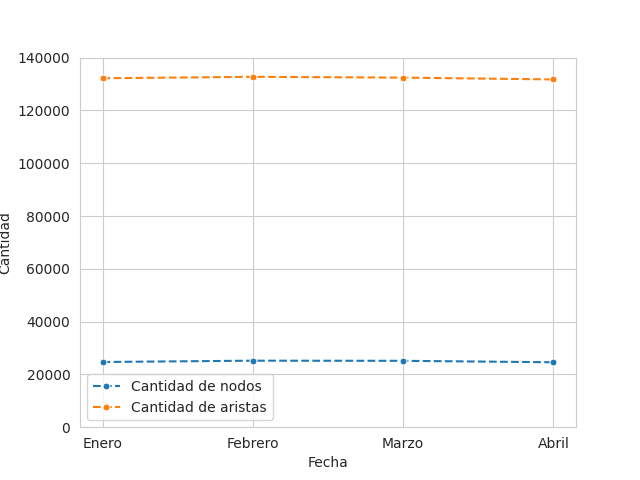
\includegraphics[width=0.7\textwidth]{img/resultados/cantidad_ases_rel_ribs.png}
%     \caption{Cantidad de relaciones y ASes para el primer día de los meses de enero, febrero, marzo y abril.}
%     \label{fig:cantidad_ases_rel_ribs}
% \end{figure}

\newpage
\begin{figure}[h]
    \centering
    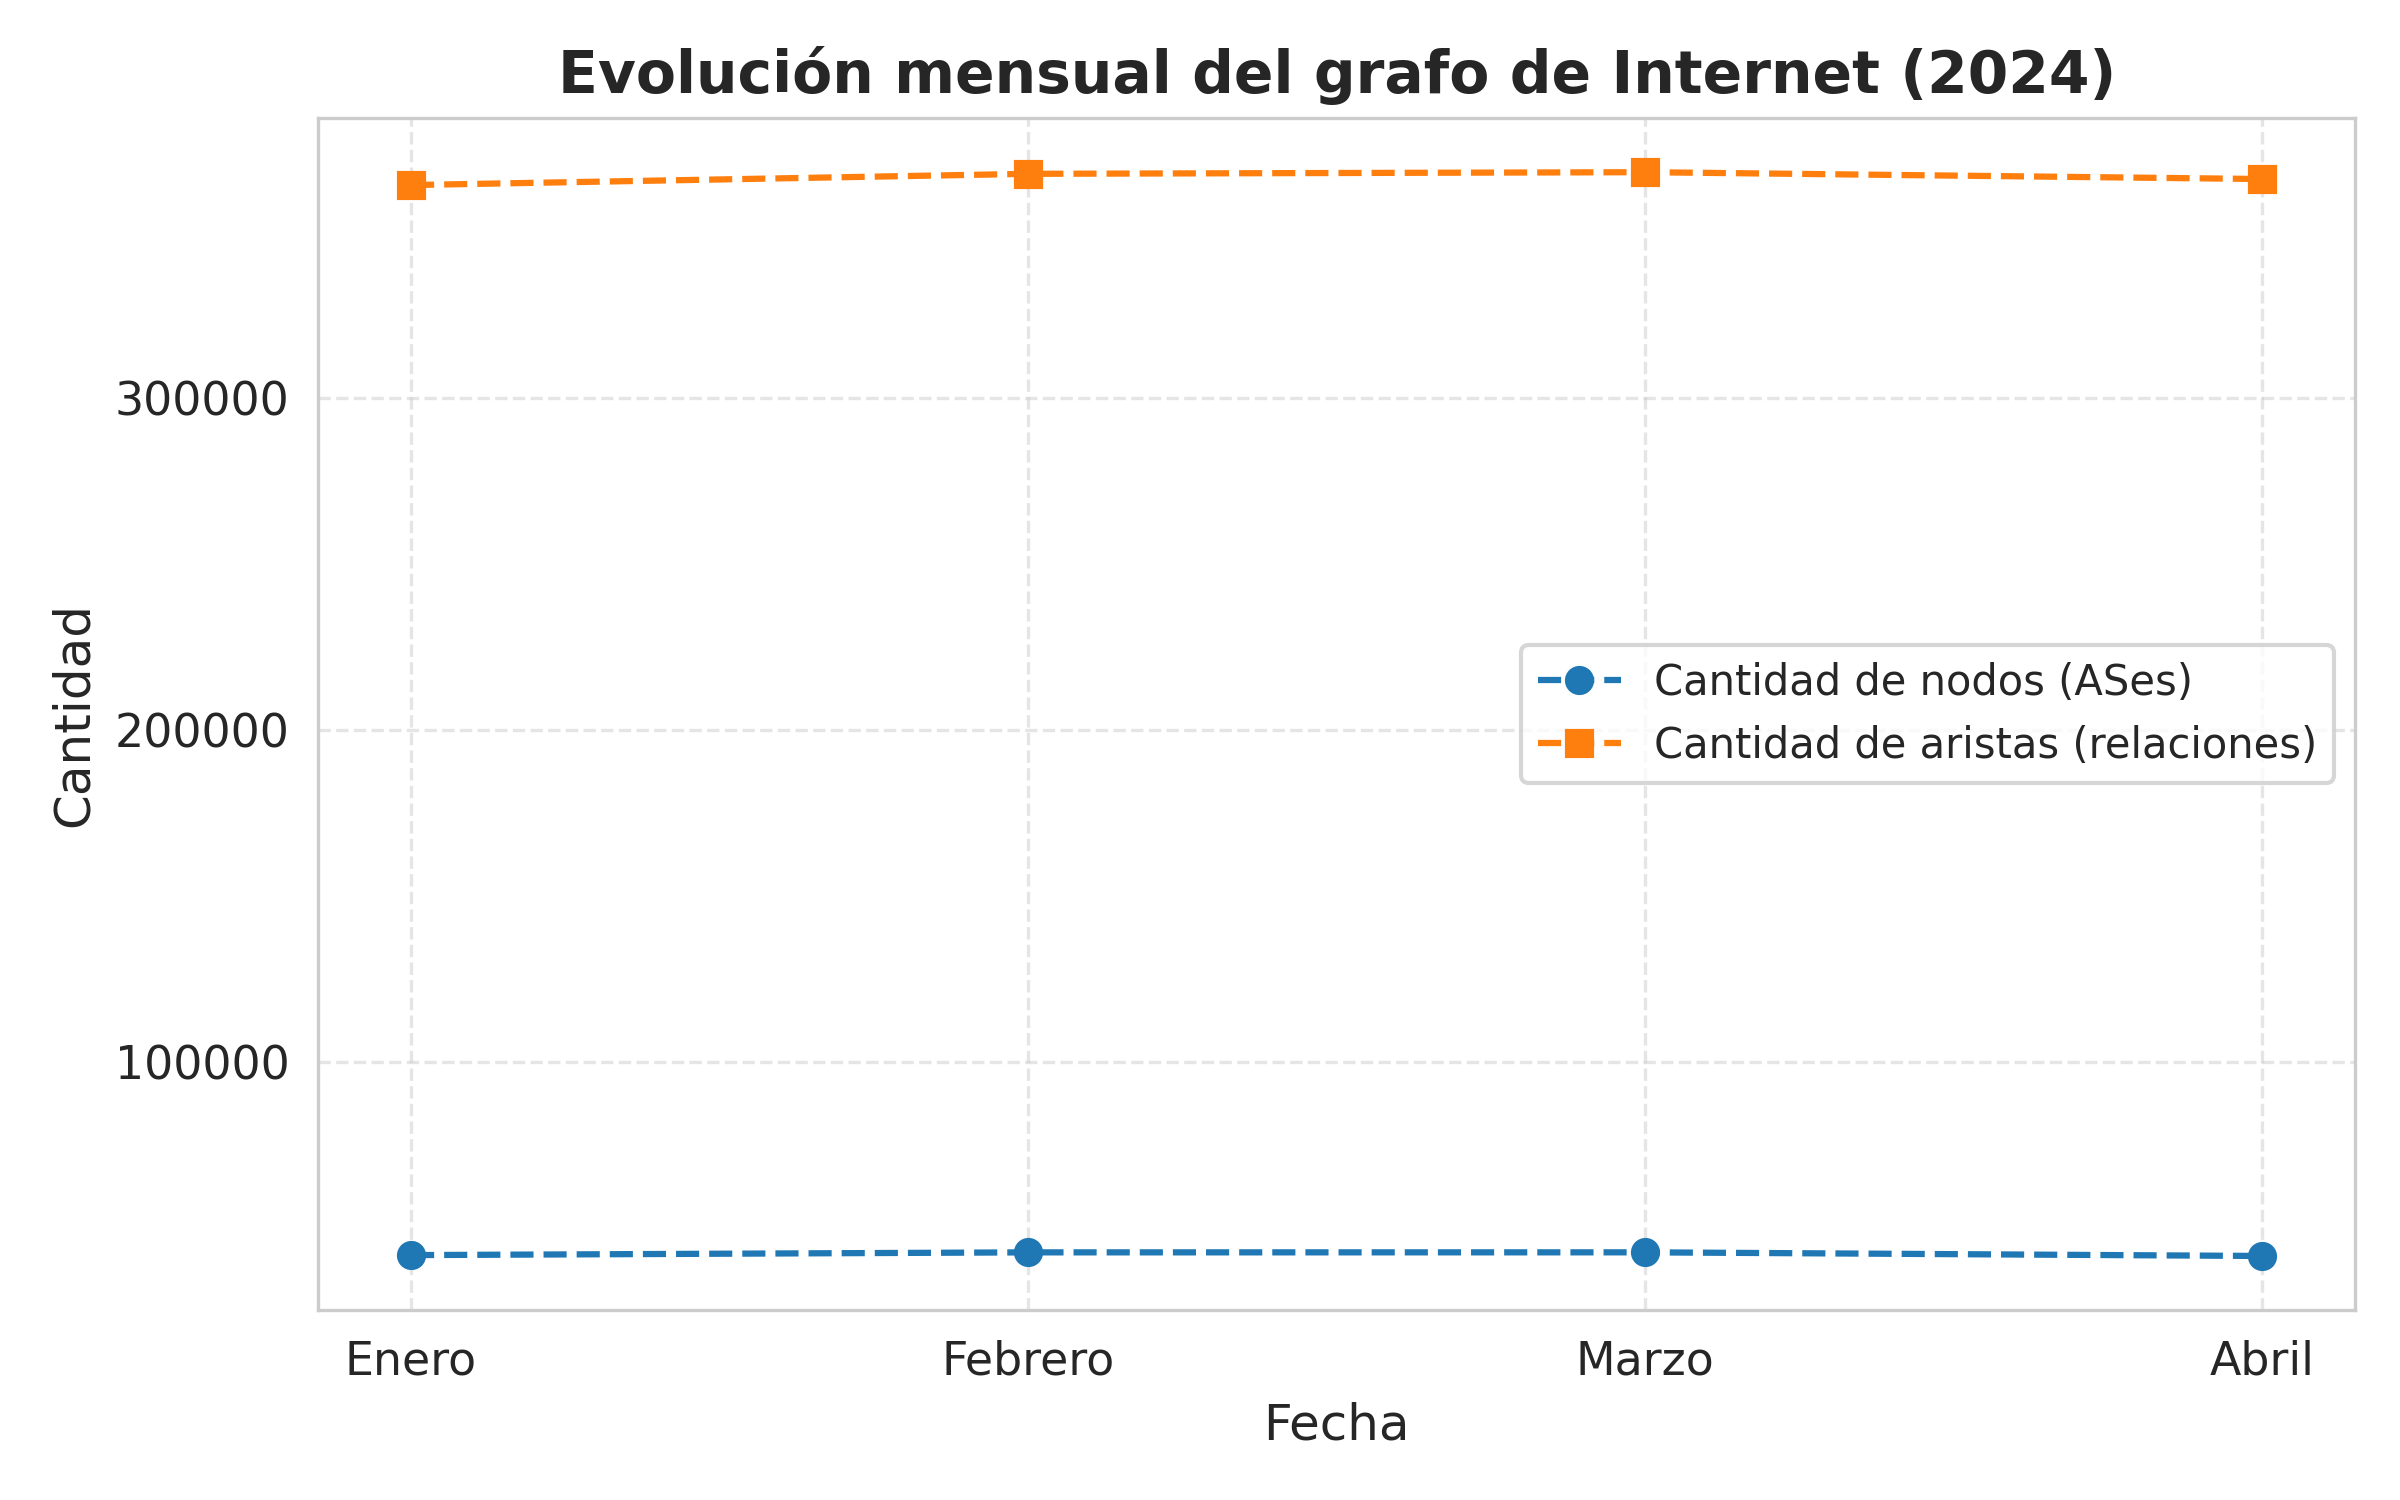
\includegraphics[width=0.9\textwidth]{img/resultados/cantidad_nodos_aristas_mensual.png}
    \caption{Cantidad de relaciones y ASes para los meses de enero a abril.}
    \label{fig:cantidad_nodos_aristas_mensual}
\end{figure}






% Para ver si utilizar únicamente las primeras 12 horas de cada mes generaba una pérdida de información, se extrajeron las RIBs correspondientes al día completo para los mismos meses. Esto permitió comparar la cantidad total de relaciones y ASes observados cuando se considera un mayor volumen de datos. Los resultados de esta comparación se presentan en la Figura~\ref{fig:cantidad_ases_rel_ribs_dia_completo}.

% \begin{figure}[H]
%     \centering
%     \includegraphics[width=0.9\textwidth]{img/resultados/cantidad_ases_rel_ribs_dia_completo.png}
%     \caption{.}
% \label{fig:cantidad_ases_rel_ribs_dia_completo}
% \end{figure}


% % TODO: Completar bien los datos
% \begin{table}[H]
%     \centering
%     \begin{tabular}{lcc}
%     \toprule
%     \textbf{Mes} & \textbf{Número de ASes} & \textbf{Número de Enlaces} \\
%     \midrule
%     Enero   &  24.696 & 227.260 \\ %FIX: Arrrgelar valor nodos
%     Febrero &  25.196 & 225.252 \\  %FIX: Arrrgelar valor nodos
%     Marzo   &  25.145 & 225.488 \\ %FIX: Arrrgelar valor nodos
%     Abril   &  26.543 & 226.541 \\ 
%     \end{tabular}
%     \caption{Cantidad de Ases y enlaces extraídos a partir de las RIBs extraídas.}
%     \label{tab:rib_datasets}
% \end{table}




\begin{table}[htbp]
\centering
\begin{tabular}{lrrrrrr}
\toprule
Mes & Nodos & Aristas & Densidad & Grado promedio & AS nuevos & AS retirados \\
\midrule
Enero    & 41.857 & 364.083 & 0.000208 & 8.70 & 0    & 0    \\
Febrero  & 42.683 & 367.470 & 0.000202 & 8.61 & 1.930 & 1.104 \\
Marzo    & 42.691 & 367.963 & 0.000202 & 8.62 & 211  & 203  \\
Abril    & 41.594 & 365.903 & 0.000212 & 8.80 & 1.213 & 2.310 \\
\bottomrule
\end{tabular}
\caption{Métricas mensuales extraídas de las RIBs BGP.}
\label{tab:caracteristicas_ribs_por_mes}
\end{table}


En la Tabla~\ref{tab:caracteristicas_ribs_por_mes} se observa la baja densidad de los grafos construidos a partir de las RIBs mensuales, la cual se mantiene en torno a 0.0002, lo cual es esperable en redes de gran escala como la de Internet, donde cada Sistema Autónomo se conecta a una fracción pequeña del total de nodos. Sin embargo, a pesar de la baja densidad, el grado promedio se mantiene estable entre 8.6 y 8.8, lo que sugiere que los ASes más relevantes continúan sosteniendo una conectividad considerable dentro de la red.\\




Para los fines de este trabajo, se consideraron como ASes Tier-1 a los siguientes: 174, 6461, 701, 1299, 3491, 3320, 6762, 7018, 12956, 6830, 6453, 5511, 3356, 3257, 2914, 2828, 1239, 286 y 209 (Para más información sobre estos ASes en la Tabla~\ref{tab:tier_1_ases} en el Anexo). La selección se basa en listas comúnmente aceptadas por la comunidad técnica~\cite{wikipedia_tier1}, las cuales identifican esos ASes como Tier-1 debido a su rol central en la infraestructura de Internet y la capacidad que tienen para llegar a cualquier destino sin pagar tránsito. Si bien no existe una definición oficial estricta, esta clasificación es usada ampliamente en estudios y repositorios públicos. En el contexto de este trabajo, fue necesario establecer este conjunto debido a que los métodos del \textit{benchmark} utilizan este listado para tomar decisiones de inferencia.



% Explicación siguientes grafos
En la Figura~\ref{fig:rel-tier1-ribs} se muestran las relaciones con al menos un AS Tier-1 en las RIBs recolectadas, mientras que la Figura~\ref{fig:rel-tier1} presenta el mismo análisis en AS Rank. Aunque AS Rank presenta una mayor cantidad de relaciones, en ambos casos se mantiene una proporción similar entre relaciones con y sin Tier-1, lo que podría indicar que nuestra extracción de RIBs conserva la estructura observada de Internet por AS Rank.\\


La diferencia en cantidad podría deberse al hecho de que las RIBs utilizadas corresponden a las primeras 12 horas del primer día de cada mes, lo que limita la visibilidad completa de las relaciones existentes. Esta restricción afecta principalmente a las relaciones entre ASes de niveles más bajos en la jerarquía de Internet, ya que estas suelen aparecer con menor frecuencia en las rutas BGP recolectadas. Por el contrario, las relaciones que involucran ASes Tier-1 las cuales tienen un rol más central en la infraestructura y por ende tienden a repetirse en múltiples rutas, ya que desde ellos es posible alcanzar cualquier otro punto de la red. En consecuencia, al capturar solo una fracción de las RIBs, se espera observar una menor proporción de relaciones que no incluyen ASes Tier-1.

\begin{figure}[ht]
    \centering
    
    \begin{subfigure}[b]{0.45\textwidth}
        \centering
        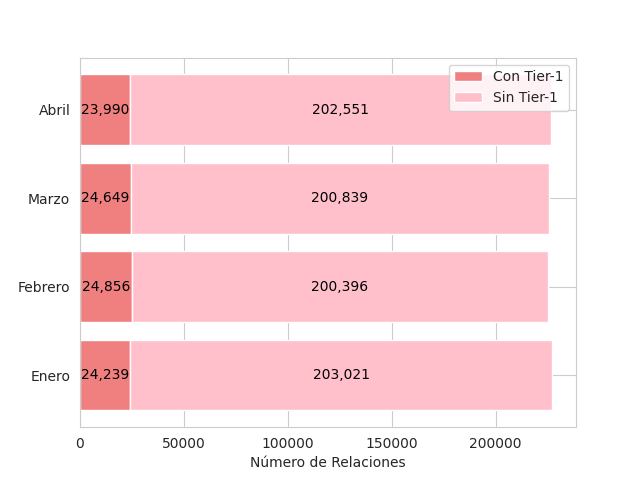
\includegraphics[width=\textwidth]{img/resultados/relaciones_con_tier1_ribs.png}
        \caption{Relaciones con al menos un AS Tier-1 en RIBs extraídas.}
        \label{fig:rel-tier1-ribs}
    \end{subfigure}
    \hfill
    \begin{subfigure}[b]{0.45\textwidth}
        \centering
        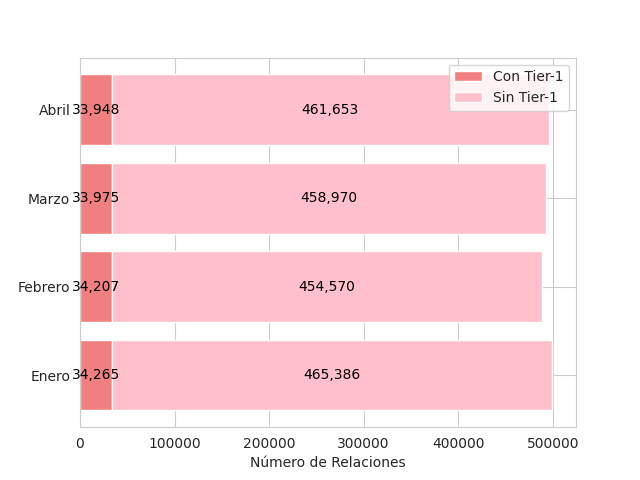
\includegraphics[width=\textwidth]{img/resultados/relaciones_con_tier1_asrank.png}
        \caption{Relaciones con al menos un AS Tier-1 en AS Rank.}
        \label{fig:rel-tier1}
    \end{subfigure}
    \caption{Comparación de relaciones que incluyen ASes Tier-1 entre RIBs recolectadas y AS Rank.}
\end{figure}

%Al analizar el grado de los ASes, es decir, la cantidad de conexiones directas que cada Sistema Autónomo (AS) mantiene con otros, es posible obtener una visión general de la estructura de conectividad en la red. Dado que las conexiones fueron extraídas de las RIBs, las cuales representan rutas hacia distintos destinos, se observa que todos los ASes tienen al menos una conexión de llegada (in-degree), pero no necesariamente una de salida (out-degree). Esto se debe a que cada ruta registrada en las RIBs describe un camino hacia un AS, lo que garantiza que cada uno de los ASes presentes haya sido alcanzado por al menos una ruta. \\



En las Figuras~\ref{fig:distribucion_as_grado_salida_entrada_febrero_boxplot_con_outliers} y \ref{fig:distribucion_as_grado_salida_febrero_boxplot_sin_outliers} se puede observar que son pocos los Sistemas Autónomos que cuentan con un número significativamente mayor de conexiones en comparación con el resto. Al graficar la distribución sin estos valores (outliers), resulta más fácil reconocer los cuartiles y comprender la dispersión de los datos, donde se aprecia que la mayoría de los ASes mantiene entre dos y cuatro relaciones salientes.
Esto se confirma en la Figura~\ref{fig:distribucion_as_grado_salida_entrada_febrero_log}, que muestra la distribución logarítmica del número de relaciones. En ella se evidencia una distribución de cola larga (\textit{long tail}), en la cual la gran mayoría de los ASes presenta un grado bajo, mientras que unos pocos concentran una cantidad desproporcionalmente alta  de conexiones. Este patrón es característico de redes jerárquicas  y sugiere que la topología AS-level de Internet sigue una distribución tipo ley de potencia (\textit{power-law}), donde un reducido número de nodos cumple un rol central de interconectividad.\\

\begin{figure}[H]
    \centering

    \begin{subfigure}[b]{0.48\textwidth}
        \centering
        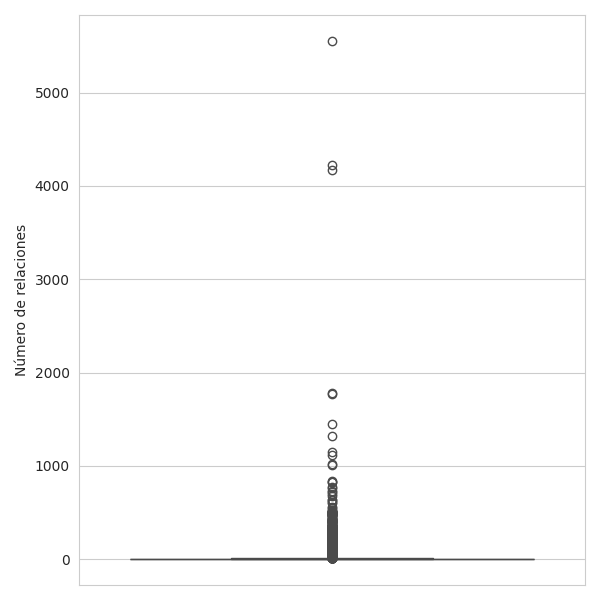
\includegraphics[width=\textwidth]{img/resultados/distribucion_as_grado_salida_febrero_boxplot_con_outliers.png}
        \caption{Distribucion de cantidad de aristas a un AS con outliers.}
        \label{fig:distribucion_as_grado_salida_entrada_febrero_boxplot_con_outliers}
    \end{subfigure}
    \hfill
    \begin{subfigure}[b]{0.48\textwidth}
        \centering
        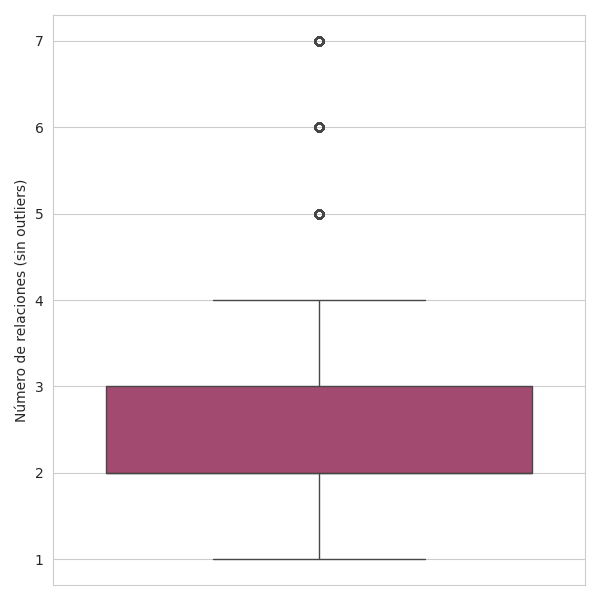
\includegraphics[width=\textwidth]{img/resultados/distribucion_as_grado_salida_entrada_febrero_boxplot_sin_outliers.png}
        \caption{Distribución de cantidad de aristas a un AS sin outliers.}
        \label{fig:distribucion_as_grado_salida_febrero_boxplot_sin_outliers}
    \end{subfigure}


    % Segunda fila: tercera subfigura
    \begin{subfigure}[b]{0.7\textwidth}
        \centering
        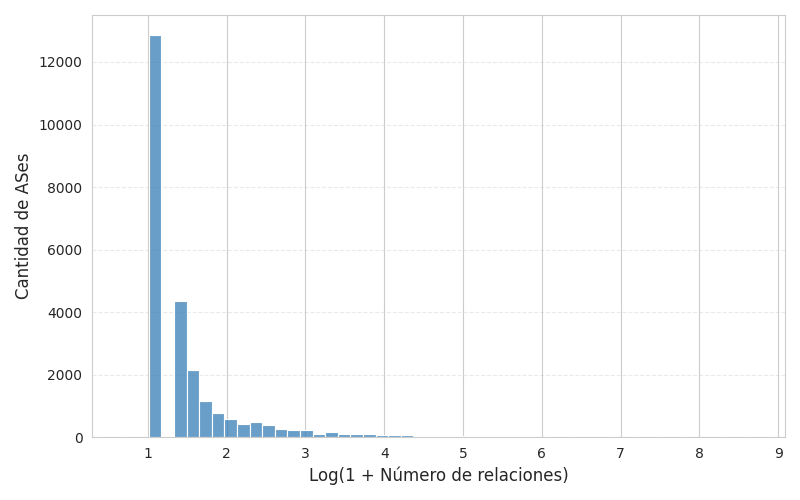
\includegraphics[width=\textwidth]{img/resultados/distribucion_as_grado_salida_entrada_febrero_log.png}
        \caption{Distribución en escala logarítmica.}
        \label{fig:distribucion_as_grado_salida_entrada_febrero_log}
    \end{subfigure}


    \caption{Comparación de la distribución del grado de salida de ASes en febrero, con y sin outliers.}
    \label{fig:distribucion_as_grado}
\end{figure}


%TODO: FIjarse mejor en como se quitaron los outliers (mencionarlo)




Además, en la Figura~\ref{fig:top_20_as_febrero_numerorelaciones} se presentan los 20 Sistemas Autónomos con mayor cantidad de conexiones. En el gráfico, los ASes son Tier-1 se destacan en un tono más oscuro. Como es de esperar, esto se debe a su rol central en la topología de Internet, lo que los hace más presentes en diferentes rutas y, por tanto, atractivos para que otros ASes establezcan conexiones con ellos. Esto reafirma lo establecido previamente, que la mayoría de ASes periféricos poseen menos presencia en rutas.\\



% TODO: Buscar paper donde hable de la jerarquia y estructura del Internet :)
% (Falta decir que los otros son tipo CArrier)
\begin{figure}[t]
    \centering
    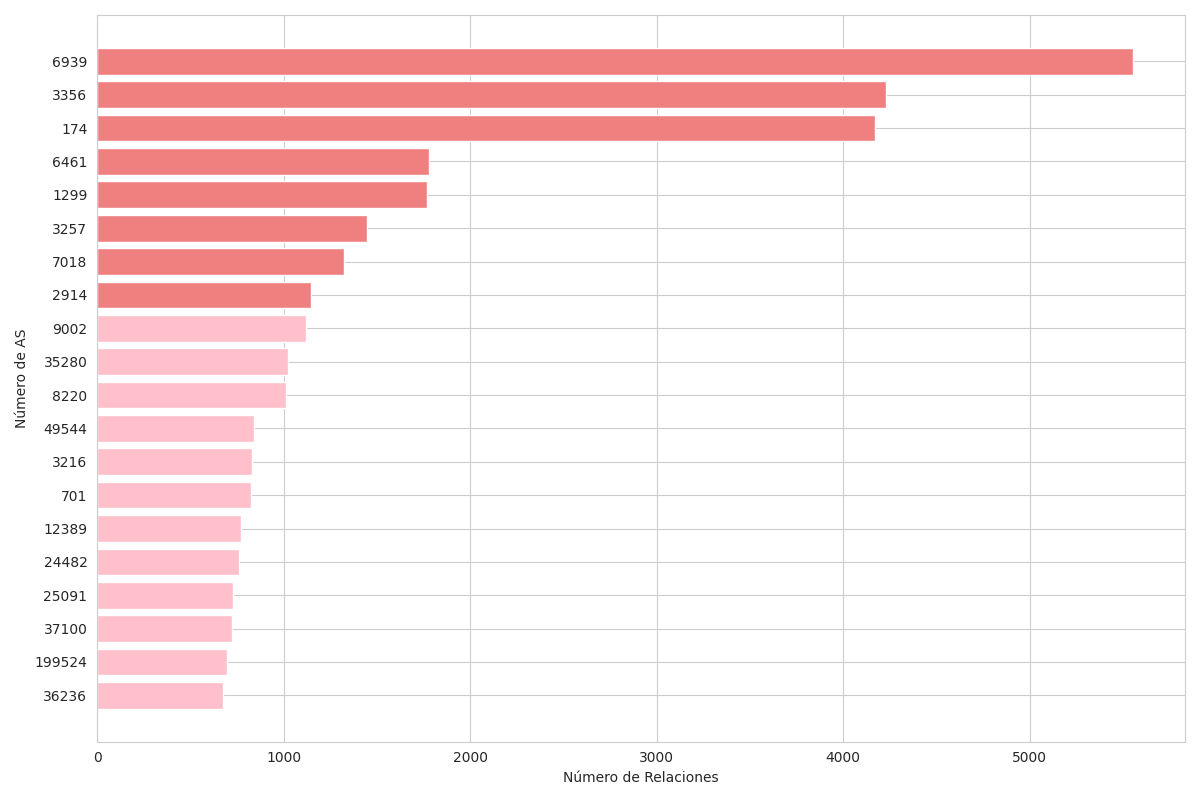
\includegraphics[width=0.7\textwidth]{img/resultados/top_20_as_febrero_numerorelaciones_src.png}
    \caption{Top 20 ASes con mayor número de conexiones (grado), para RIB de febrero 2024.}
\label{fig:top_20_as_febrero_numerorelaciones}
\end{figure}



Otro análisis que se realizó fue graficar la distribución de la longitud de las rutas BGP observadas en las RIBs (Figura~\ref{fig:distribucion_largo_path}), donde se observa una clara concentración en longitudes entre 3 y 5 Sistemas Autónomos, siendo la longitud más frecuente de 4 saltos. Esta distribución sugiere una estructura de red eficiente, donde la mayoría de los destinos pueden ser alcanzados con pocos saltos intermedios. Además, la ausencia de rutas de longitud 1 y valores atípicos evidentes, indican que el proceso de limpieza y filtrado de las rutas fue hecho de buena  manera y sin errores evidentes. Figura~\ref{fig:comparacion_mensual_largo_paths} en el Anexo presenta una comparación de esta distribución entre los distintos meses analizados.\\

\begin{figure}[H]
    \centering
    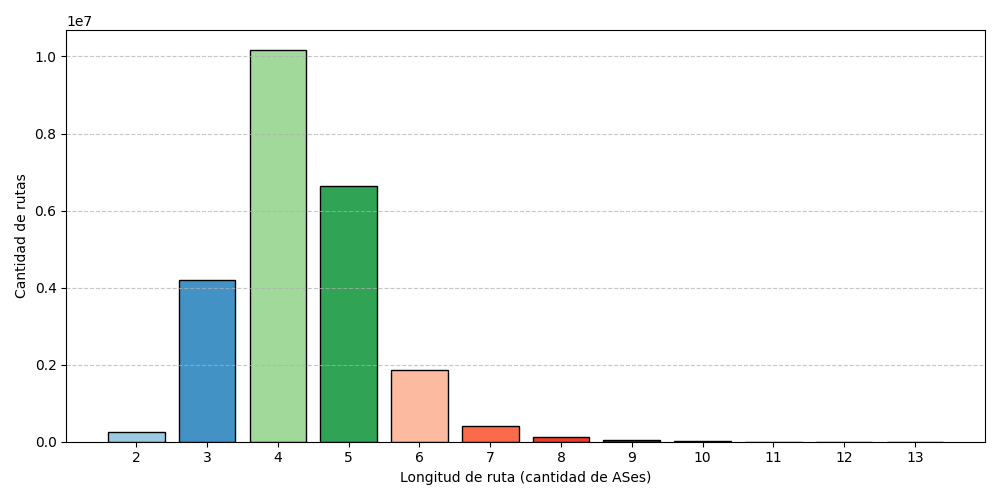
\includegraphics[width=0.7\textwidth]{img/resultados/distribucion_largo_paths.png}
    \caption{Distribución de longitud de rutas BGP.}
\label{fig:distribucion_largo_path}
\end{figure}


En la misma línea, se analizó la frecuencia con la que los ASes aparecen en las rutas BGP extraídas. Permitiendo identificar ASes que ocupan posiciones centrales dentro de la infraestructura de Internet, al participar en un gran número de caminos de enrutamiento.\\

Figura~\ref{fig:top_20_as_febrero_numerorelaciones} presenta el top 20 de Sistemas Autónomos con mayor frecuencia de aparición en las rutas BGP extraídas. Los ASes con mayor grado y por ende más conectados están destacados en color naranja. Esto refuerza la idea del rol central que desempeñan los ASes de nivel Tier-1 en la infraestructura de Internet, al combinar una alta conectividad (alto grado de conectividad) con una participación recurrente en múltiples trayectorias (alta frecuencia de aparición de múltiples caminos), evidenciando su importancia en el enrutamiento.\\


\begin{figure}[H]
    \centering
    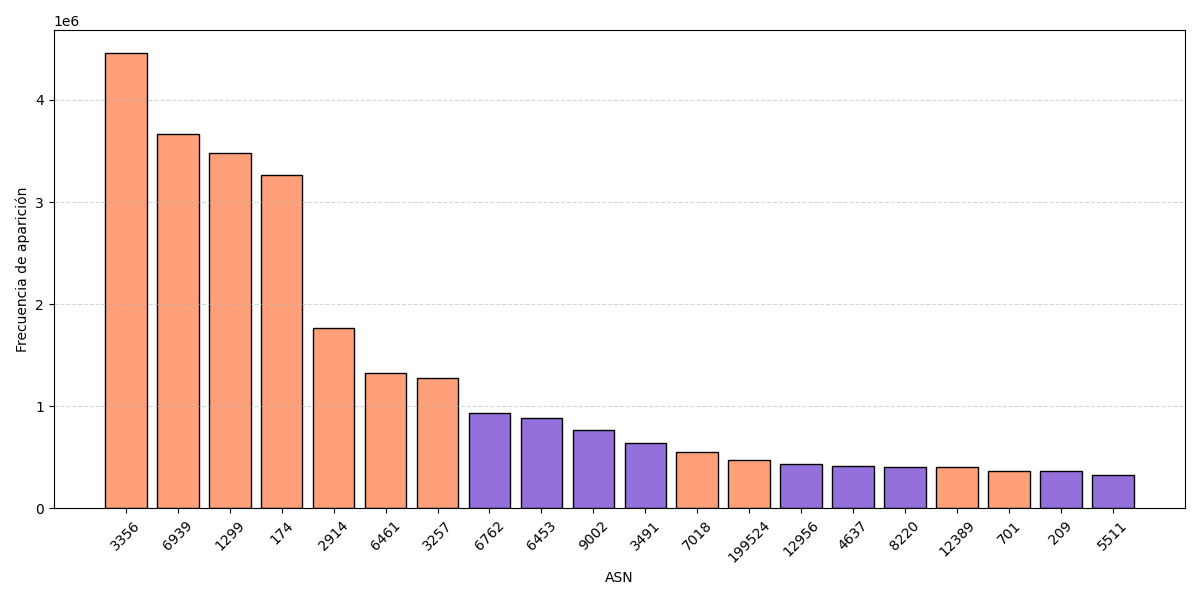
\includegraphics[width=0.8\textwidth]{img/resultados/top_20_ases_frecuencia_ribs.png}
    \caption{Top 20 ASes más frecuentes en rutas BGP (Febrero 2024).}
\label{fig:top_20_ases_frecuencia_ribs}
\end{figure}



% COMIENZO ANALICIS AS RANK ---------------------------------------------------------

%DATASET ASRANK\\

%\vspace{1cm}
\paragraph{Dataset ASRank}

%\vspace{1cm}

Para la evaluación y entrenamiento, de los métodos del \textit{benchmark} se utilizó ASRank, el cual contiene aproximadamente 76.000 Sistemas Autónomos y 499.651 enlaces. En la Tabla~\ref{tab:asrank_datasets}, ubicada en el Anexo~\ref{sec:attr_asrank_section}, se detalla la cantidad de conexiones y ASes correspondientes a los cuatro primeros meses.\\

Para complementar esta información, en la Figura~\ref{fig:cantidad_asrank_meses}  se presenta la evolución mensual del número de ASes y enlaces registrados por ASRank y la cantidad de cada tipo de relación.\\

\begin{figure}[H]
    \centering

    \begin{subfigure}[h]{0.4\textwidth}
        \centering
        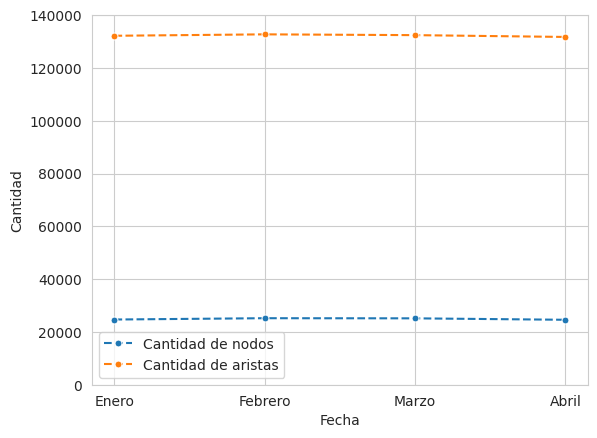
\includegraphics[width=\textwidth]{img/resultados/ribs/cantidad_nodos_aristas_por_fechaUntitled.png}
        \caption{Cantidad de ASes y relaciones extraídas de las RIBs.}
        \label{fig:cantidad_nodos_aristas_por_fecha_ribs}
    \end{subfigure}
    \hfill
    \begin{subfigure}[h]{0.50\textwidth}
        \centering
        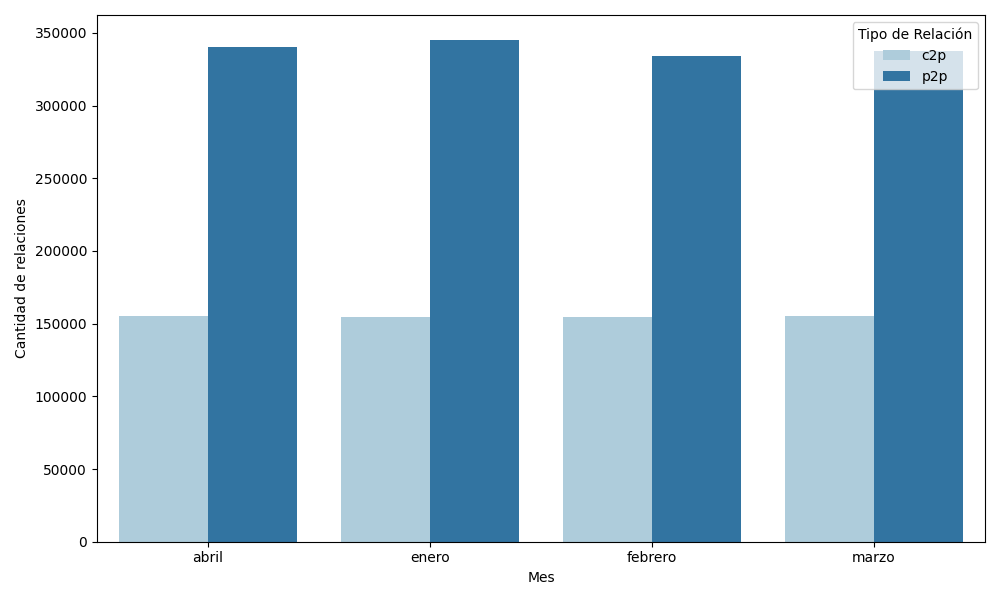
\includegraphics[width=\textwidth]{img/resultados/asrank/relaciones_por_tipo_asrank.png}
        \caption{Cantidad de relaciones por tipo según AS Rank.}
        \label{fig:relaciones_por_tipo_asrank}
    \end{subfigure}

    \caption{Cantidad de ASes, relaciones y tipos de relaciones de AS Rank para los meses de enero a abril de 2024.}
    \label{fig:cantidad_asrank_meses}
\end{figure}

\newpage
Los ASes con más relaciones C2P son en su mayoría Tier-1, como Cogent (AS174) y Lumen (AS3356), reflejando su rol como proveedores de tránsito. En contraste, los ASes con más relaciones P2P incluyen tanto Tier-1 como actores regionales o de hosting, como i3D.net (AS49544). La Tabla~\ref{tab:info_ases_top} entrega información complementaria sobre cada AS, permitiendo entender su rol en la estructura global de Internet.\\


\begin{figure}[H]
    \centering
    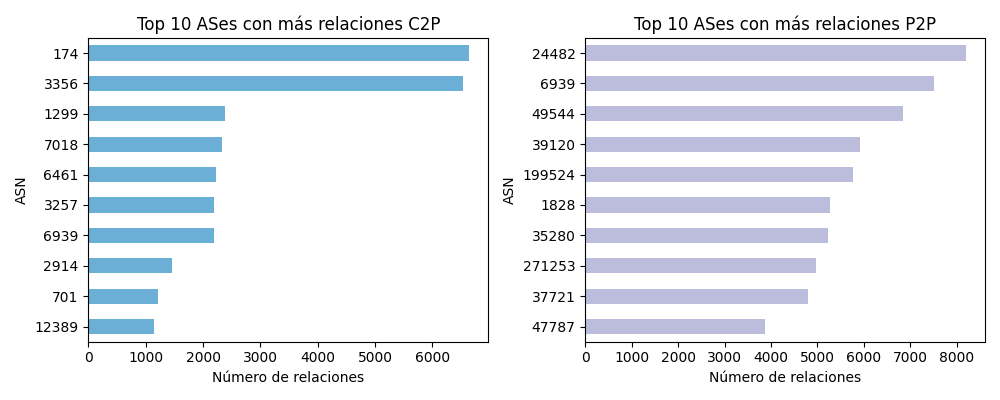
\includegraphics[width=0.9\textwidth]{img/resultados/top_ases_por_tipo_relacion.png}
    \caption{Top 10 ASes con mayor cantidad de relaciones C2P y P2P inferidas}
    \label{fig:top_ases_relaciones}
\end{figure}



Otro análisis consistió en comparar la cantidad de Sistemas Autónomos y aristas coincidentes entre los PATHs recolectados desde las RIBs y los presentes en el dataset de AS Rank. Esta comparación fue importante, ya que luego el dataset de AS Rank se ocupó para etiquetar los enlaces presentes en la topología. En la Figura~\ref{fig:aristas_coincidentes_por_mes_con_ribs} se muestra la cantidad de coincidencias de ASes y aristas por mes.\\


\begin{figure}[H]
    \centering
    \begin{subfigure}[h]{0.40\textwidth}
        \centering
        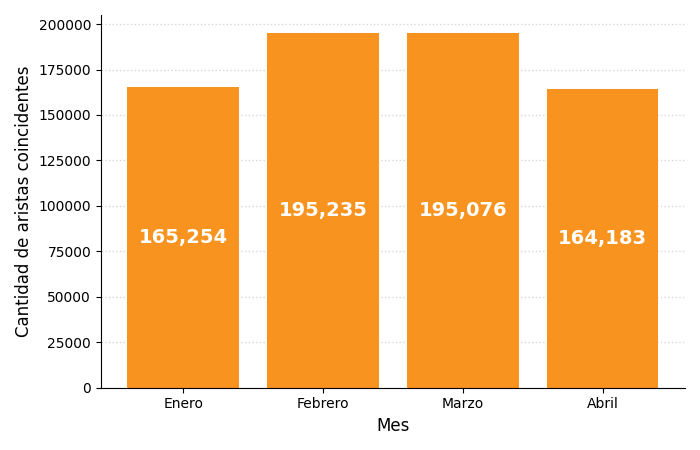
\includegraphics[width=\textwidth]{img/resultados/aristas_coincidentes_por_mes_con_ribs.png}
        \caption{Aristas coincidentes entre AS paths extraídos de las RIBs y de AS Rank.}
        \label{fig:aristas_coincidentes_por_mes_con_ribs}
    \end{subfigure}
    \hfill
    \begin{subfigure}[h]{0.40\textwidth}
        \centering
        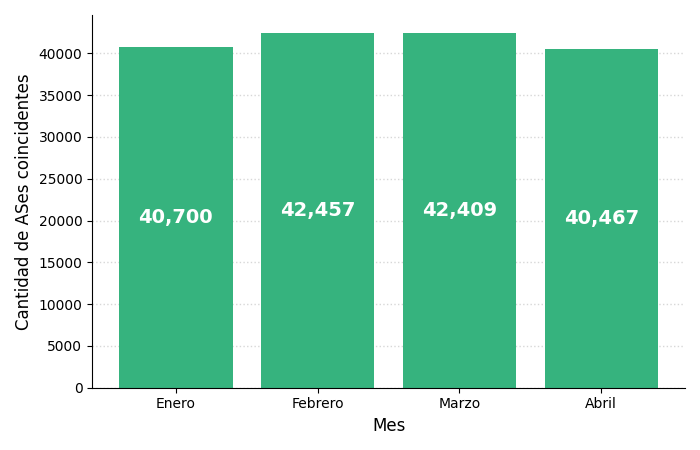
\includegraphics[width=\textwidth]{img/resultados/ases_coincidentes_por_mes_ribs.png}
        \caption{ASes coincidentes entre AS paths extraídos de las RIBs y de AS Rank.}
        \label{fig:ases_coincidentes_por_mes_ribs}
    \end{subfigure}
    \caption{Comparación de coincidencias entre RIBs recolectadas y AS Rank.}
    \label{fig:coincidencias_ribs_asrank}
\end{figure}



\begin{table}[H]
\centering
\caption{Información y clasificación de los principales ASes observados.}
\label{tab:info_ases_top}
\resizebox{\textwidth}{!}{
\begin{tabular}{lll}
\toprule
\textbf{ASN} & \textbf{Organización} & \textbf{Rol / Tipo} \\
\midrule
174     & Cogent Communications        & Tier-1 ISP           \\
3356    & Level 3 / Lumen              & Tier-1 ISP           \\
1299    & Arelion (ex Telia)           & Tier-1 ISP           \\
7018    & AT\&T Services               & Tier-1 ISP           \\
6461    & Zayo Group                   & Tier-1 ISP           \\
3257    & GTT Communications           & Tier-1 ISP           \\
6939    & Hurricane Electric           & Tier-1 ISP           \\
2914    & NTT America                  & Tier-1 ISP           \\
701     & Verizon Business             & Tier-1 ISP           \\
12389   & Rostelecom                   & Tier-1 nacional      \\
\midrule
24482   & SG.GS (Singapur)             & Hosting / Peer       \\
49544   & i3D.net (Holanda)            & Gaming / Hosting     \\
39120   & Consoltech (Europa del Este) & Datacenter           \\
199524  & MivoCloud (Moldavia)         & ISP regional         \\
1828    & Telenor (Noruega)            & ISP nacional         \\
35280   & Omantel                      & ISP nacional         \\
271253  & Empresa Argentina de Soluciones Satelitales (ARSAT) & ISP nacional \\
37721   & Safaricom (Kenia)            & ISP nacional         \\
47787   & Hosting Ukraine Ltd          & Hosting / Peer       \\
\bottomrule
\end{tabular}
}
\end{table}



%/////////////////////////////////////////////////
%/////////////////////////////////////////////////
%/////////////////////////////////////////////////
\vspace{0.5cm}
\section{Resultados del uso de Redes Neuronales de Grafos (GNNs)} \label{sec:gnn_result_section}

Como se mencionó previamente, para el uso de modelos GNN se exploraron dos enfoques: el \textbf{entrenamiento \textit{por etapas}} (Sección~\ref{sec:resultados_entrenamiento_por_etapas}) y el \textbf{entrenamiento \textit{end-to-end}} (Sección~\ref{sec:entrenamiento_end_to_end}).
A continuación se presenta una descripción de los experimentos y sus respectivos resultados.\\

%Las métricas utilizadas para evaluar los modelos se definen a continuación. 
%La \textbf{Accuracy} corresponde a la exactitud global, calculada como la proporción de instancias correctamente clasificadas sobre el total de ejemplos. 
%Por otro lado, las métricas de \textbf{Precision} y \textbf{Recall} se reportan como \textit{micro-promedio}, es decir, considerando de manera conjunta los verdaderos positivos (TP), falsos positivos (FP) y falsos negativos (FN) de todas las clases como si se tratara de un único problema binario, para luego aplicar las fórmulas correspondientes:

%\[
%\text{Precision}_{micro} = \frac{\sum_{i=1}^C TP_i}{\sum_{i=1}^C (TP_i + FP_i)}
%\]

%\[
%\text{Recall}_{micro} = \frac{\sum_{i=1}^C TP_i}{\sum_{i=1}^C (TP_i + FN_i)}
%\]

%\[
%\text{Accuracy} = \frac{\sum_{i=1}^C TP_i}{\sum_{i=1}^C (TP_i + FP_i + FN_i + TN_i)}
%\]

%donde \(C\) corresponde al número de clases consideradas.

%/////////////////////////////////////////////////

\subsection{Resultados de Entrenamiento \textit{Por Etapas}} \label{sec:resultados_entrenamiento_por_etapas}

En este enfoque, el aprendizaje se divide en dos fases separadas: primero se generan \textit{embeddings} para cada nodo del grafo, y luego estos \textit{embeddings} se utilizan como entrada para un modelo de clasificación. El flujo de trabajo fue el siguiente:


\begin{enumerate}
    \item Importación de RIBs y construcción del grafo DGL.
    \item Asociación de atributos a cada nodo, siguiendo los mismos tres casos mencionados anteriormente.
    \item Generación de representaciones vectoriales para cada AS mediante un modelo GNN entrenado para una tarea auxiliar. Se evaluaron dos estrategias principales:
    \begin{itemize}
        \item Inferencia de la existencia de conexiones entre nodos (tarea de predicción de enlaces).
        \item Inferencia de características específicas de los ASes a partir de su contexto en el grafo (por ejemplo, clasificación o clustering).
    \end{itemize}
    \item Uso de los \textit{embeddings} obtenidos como entrada para un modelo MLP que predice la relación entre pares de ASes.
\end{enumerate}

Dado el desbalance de clases en el dataset, en todos los experimentos se evaluaron con y sin balance de clases, así como con entrenamiento con el grafo completo y por batches. Además, cada caso fue probado utilizando los tres tipos de encoder (GCN, GraphSAGE y GAT) y ambos decoders (MLP y producto punto), para ver su comportamiento.\\

A continuación, se presentan los diferentes experimentos creados con este enfoque.\\



%/////////////////////////////////////////////////
\subsubsection{Caso 0: Predicción de enlaces utilizando grafo con atributos de nodos extraídos de PeeringDB}

\begin{itemize}
    \item \textbf{RIBs:} Febrero 2024.
    \item \textbf{Atributos de nodos:} Dataset creado a partir de PeeringDB.
   \item \textbf{Tarea para la creación de \textit{embeddings}:} Determinar la existencia o no de un enlace entre pares de nodos (Sistemas Autónomos).
    \item \textbf{Tamaño \textit{embeddings}:} 32.
    \item \textbf{Epochs:} 100 (GNN) y 20 (ANN).
    \item \textbf{Early Stopping:} Paciencia de 8 epochs.
    \item \textbf{Learning Rate:} 0.001 (GNN) y 0,001 (ANN).
\end{itemize}




% decir q se crearon aristas grafo ngativo

A continuación, los resultados obtenidos a partir de la tarea para crear \textit{embeddings}. La Tabla~\ref{tab:comparacion_accuracy_caso0} resume los valores de AUC y Accuracy alcanzados por cada combinación de encoder y decoder, mientras que la Figura \ref{fig:partes_caso_0_comparacion_roc_auc} presenta las curvas ROC asociadas, lo que permite contrastar visualmente el desempeño de cada variante.\\

\begin{figure}[H]
    \centering
    % Primera fila
    \begin{subfigure}[b]{0.45\textwidth}
        \centering
        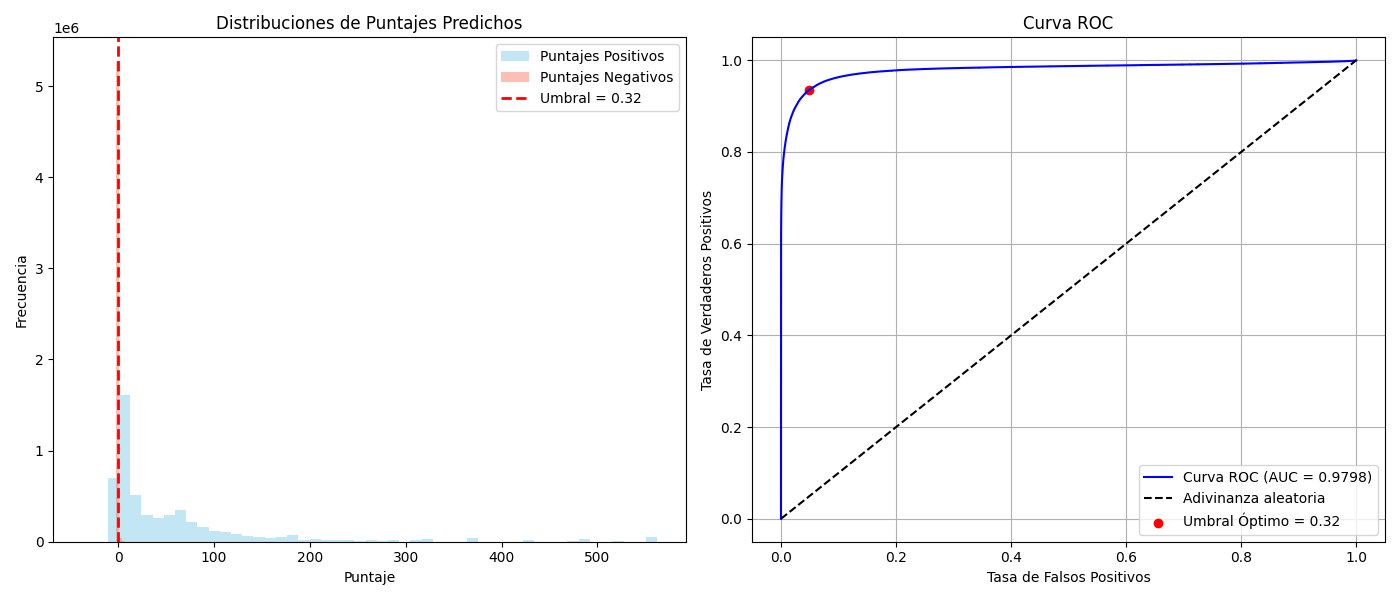
\includegraphics[width=\textwidth]{img/resultados/gnn/partes/caso2_mis_attr/resultados/roc_curve_GCN_DotProduct_mis_attr_febrero.png}
        \caption{GCN + Producto Punto}
        \label{fig:conf_matrix_gcn_dp}
    \end{subfigure}
    \hfill
    \begin{subfigure}[b]{0.45\textwidth}
        \centering
        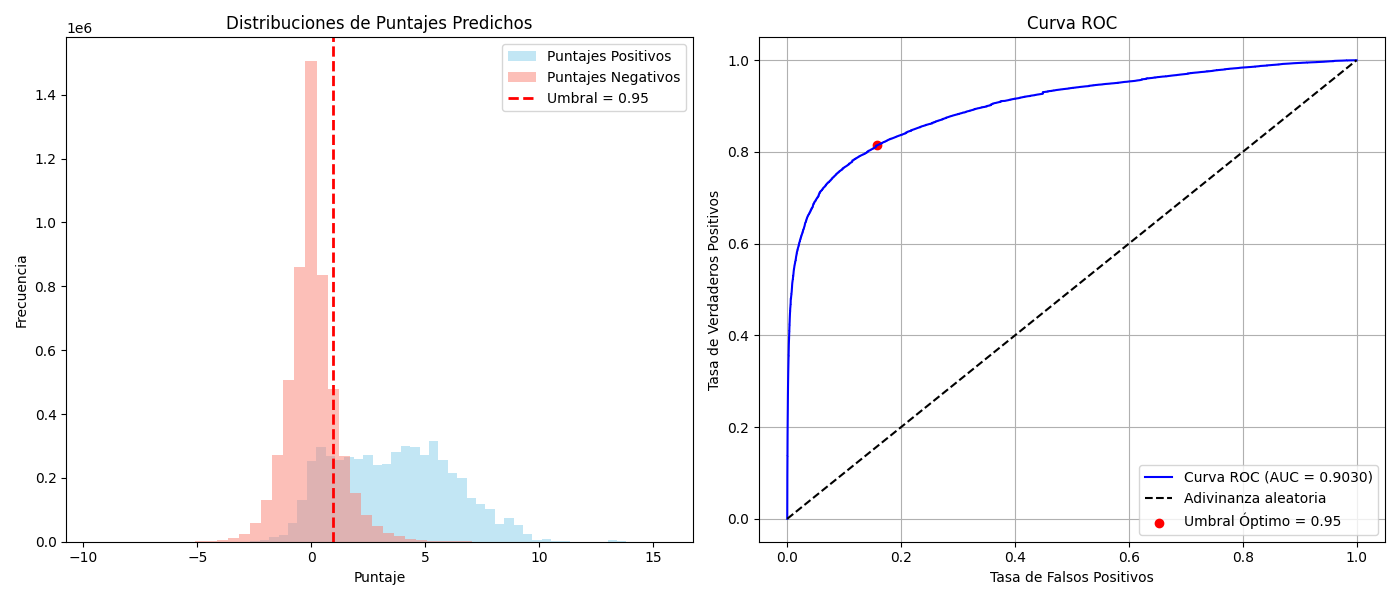
\includegraphics[width=\textwidth]{img/resultados/gnn/partes/caso2_mis_attr/resultados/roc_curve_GraphSAGE_DotProduct_mis_attr_febrero.png}
        \caption{GraphSAGE + Producto Punto}
        \label{fig:conf_matrix_sage_dp}
    \end{subfigure}

    \vspace{0.5cm}

    % Segunda fila
    \begin{subfigure}[b]{0.45\textwidth}
        \centering
        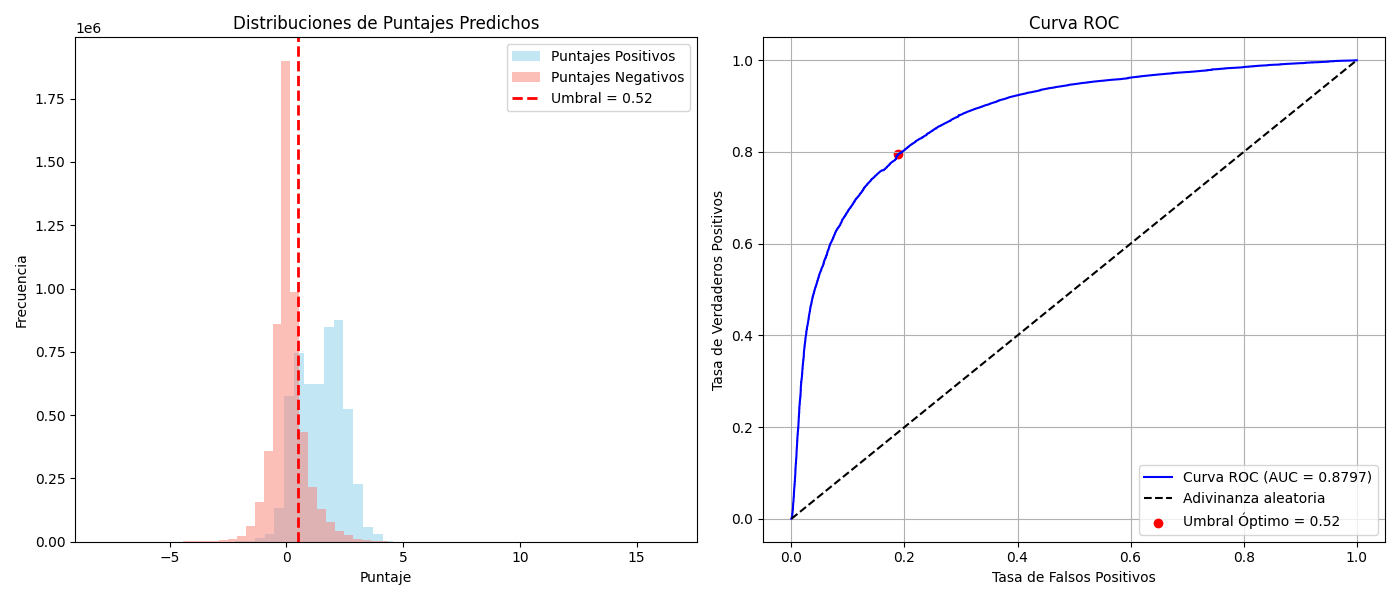
\includegraphics[width=\textwidth]{img/resultados/gnn/partes/caso2_mis_attr/resultados/roc_curve_GAT_DotProduct_mis_attr_febrero.png}
        \caption{GAT + Producto Punto}
        \label{fig:conf_matrix_gat_dp}
    \end{subfigure}
    \hfill
    \begin{subfigure}[b]{0.45\textwidth}
        \centering
        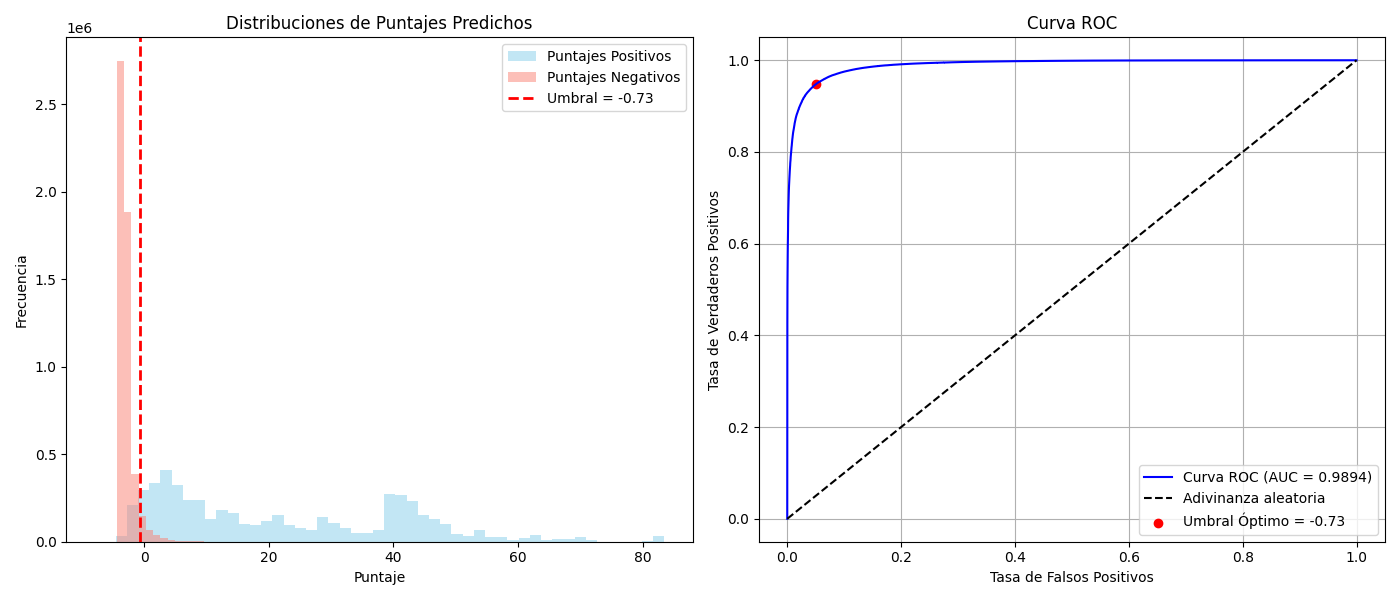
\includegraphics[width=\textwidth]{img/resultados/gnn/partes/caso2_mis_attr/resultados/roc_curve_GCN_MLP_mis_attr_febrero.png}
        \caption{GCN + MLP}
        \label{fig:conf_matrix_gcn_mlp}
    \end{subfigure}

    \vspace{0.5cm}

    % Tercera fila
    \begin{subfigure}[b]{0.45\textwidth}
        \centering
        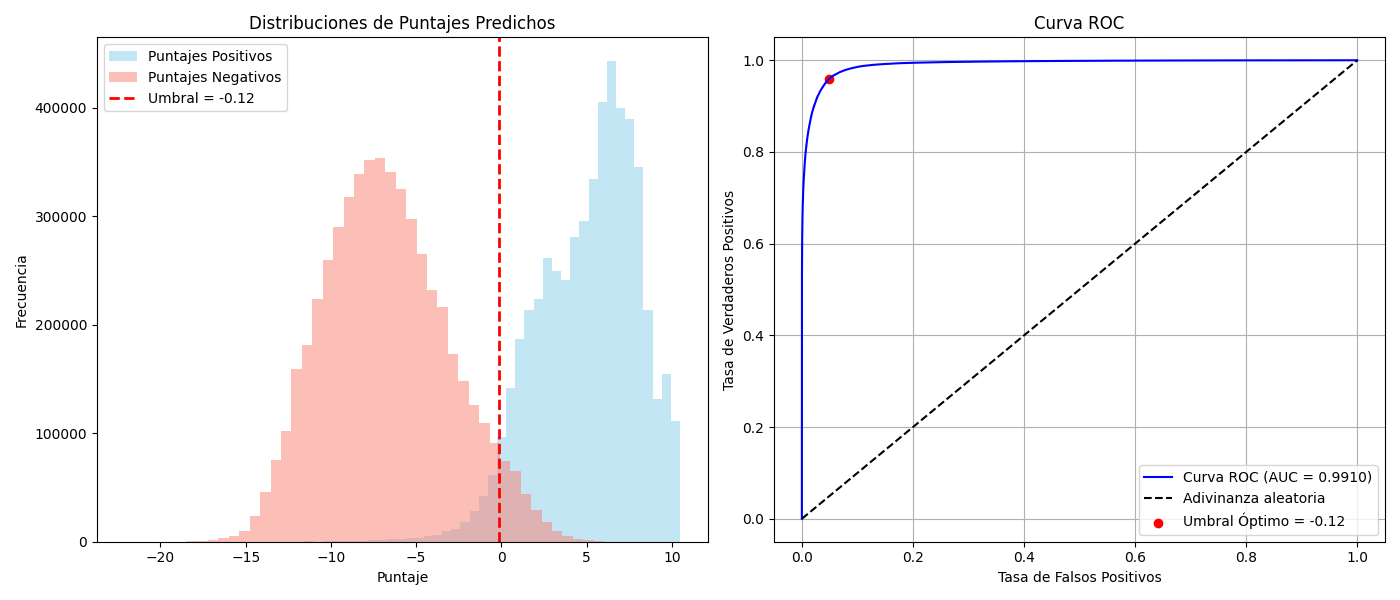
\includegraphics[width=\textwidth]{img/resultados/gnn/partes/caso2_mis_attr/resultados/roc_curve_GraphSAGE_MLP_mis_attr_febrero.png}
        \caption{\textbf{GraphSAGE + MLP}}
        \label{fig:conf_matrix_sage_mlp}
    \end{subfigure}
    \hfill
    \begin{subfigure}[b]{0.45\textwidth}
        \centering
        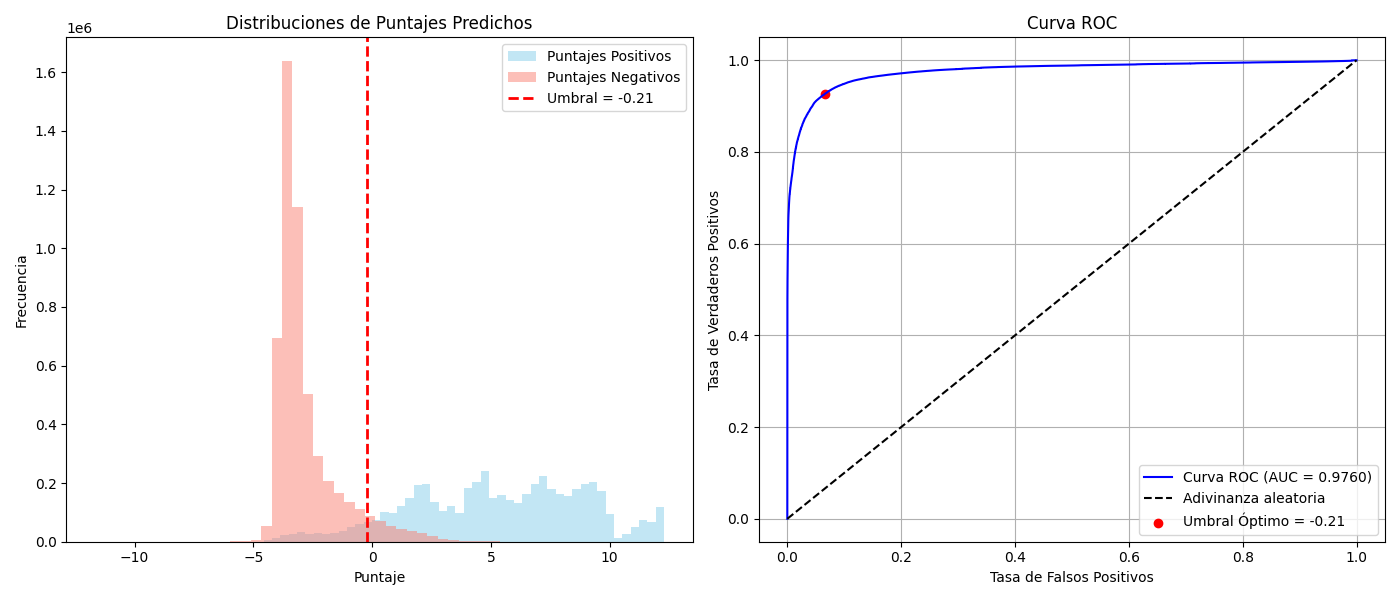
\includegraphics[width=\textwidth]{img/resultados/gnn/partes/caso2_mis_attr/resultados/roc_curve_GAT_MLP_mis_attr_febrero.png}
        \caption{GAT + MLP}
        \label{fig:conf_matrix_gat_mlp}
    \end{subfigure}

    \caption{Curvas ROC y distribución de los resultados.}
    \label{fig:partes_caso_0_comparacion_roc_auc}
\end{figure}

En todos los modelos (GCN, GraphSAGE y GAT), el decodificador MLP supera a Dot Product. Esto sugiere que un decodificador más expresivo es capaz de capturar mejor las relaciones entre los ASes. En contraste, el Dot Product es un decodificador simple que solo mide la “similitud” entre vectores, lo que puede resultar insuficiente para esta tarea.



\begin{table}[H]
    \centering
    \begin{tabular}{lccc}
    \hline
    \textbf{Modelo} & \textbf{Decodificador} & \textbf{AUC}& \textbf{Accuracy (\%)} \\
    \hline
    GCN & Dot Product &  0.986 & 0.945 \\
    GraphSAGE & Dot Product & 0.913 &  0.835\\
    GAT & Dot Product & 0.887 & 0.840 \\
    GCN & MLP  & 0.991 & 0.952 \\
    \textbf{GraphSAGE} & \textbf{MLP}  & \textbf{0.991} & \textbf{0.958} \\
    GAT & MLP &  0.967 & 0.916 \\
    \hline
    \end{tabular}
    \caption{Accuracy de la inferencia con link prediction para la creación de \textit{embeddings}.}
    \label{tab:comparacion_accuracy_caso0}
\end{table}

\newpage
Luego de la generación de \textit{embeddings}, se evaluó la tarea principal. En la Tabla~\ref{tab:accuracy_gnn_variants_caso0} se muestran los resultados de Accuracy obtenidos para cada combinación de encoder y decoder. Las cuales consisten en: sin batching y sin balanceo (`NoBatch-NoW'), sin batching pero con balanceo (`NoBatch-W'), con batching sin balanceo (`Batch-NoW'), y con ambas (`Batch-W').  \\


\begin{table}[H]
\centering
\resizebox{\textwidth}{!}{%
\begin{tabular}{llcccccccccccc}
\toprule
\multirow{2}{*}{\textbf{Modelo}} & 
\multirow{2}{*}{\textbf{Decodificador}} & 
\multicolumn{3}{c}{\textbf{NoBatch-NoW}} & 
\multicolumn{3}{c}{\textbf{NoBatch-W}} & 
\multicolumn{3}{c}{\textbf{Batch-NoW}} & 
\multicolumn{3}{c}{\textbf{Batch-W}} \\
\cmidrule(lr){3-5} \cmidrule(lr){6-8} \cmidrule(lr){9-11} \cmidrule(lr){12-14}
 & & \textbf{Precision} & \textbf{Recall} & \textbf{Accuracy} 
   & \textbf{Precision} & \textbf{Recall} & \textbf{Accuracy} 
   & \textbf{Precision} & \textbf{Recall} & \textbf{Accuracy} 
   & \textbf{Precision} & \textbf{Recall} & \textbf{Accuracy} \\
\midrule
GCN       & Dot Product &82.57&75.93&79.57&79.56&64.07&73.35&84.84&78.99&82.07&76.00&61.17&70.22\\
GraphSAGE & Dot Product &\textbf{86.08}&\textbf{83.87}&\textbf{85.04}&81.71&72.59&77.95&85.58&83.03&84.35&81.04&75.48&78.73\\
GAT       & Dot Product &85.83&81.69&83.80&79.98&71.85&76.53&86.10&83.62&84.94&79.94&73.36&77.00\\
\midrule
GCN       & MLP         &73.18&69.59&71.74&75.50&16.30&50.47&71.68&71.03&71.45&73.64&18.93&51.78\\
GraphSAGE & MLP         &82.33&76.82&79.75&79.39&53.34&70.44&78.74&74.05&76.74&76.75&44.08&65.82\\
GAT       & MLP         &79.97&74.04&77.27&64.04&38.26&60.57&76.08&71.47&74.30&66.56&32.81&59.56\\
\bottomrule
\end{tabular}}
\caption{Resultados de Precision, Recall y Accuracy (\%) por combinación de encoder y decoder bajo cuatro configuraciones: sin batching y sin balanceo (`NoBatch-NoW'), sin batching con balanceo (`NoBatch-W'), con batching sin balanceo (`Batch-NoW'), y con ambas (`Batch-W'). En negrita se indican los mejores resultados por métrica en cada configuración.}
\label{tab:accuracy_gnn_variants_caso0}
\end{table}

Podemos ver que se obtienen los mejores resultados con GraphSAGE y Dot Product como decoder, con una Accuracy de 85.04\%, diferente a lo que es de esperar, ya que para la creación de los \textit{embeddings}, con el decodificador MLP se obtuvieron los mejores resultados.\\

Esto ocurre porque para la clasificación de tipos de relación (C2P, P2P, P2C) con una ANN, lo que más importa es que los \textit{embeddings} sean bien estructurados y fáciles de separar. Aquí, el decoder Dot Product tiende a generar \textit{embeddings} más simples, lo que termina beneficiando la tarea final. Por otro lado, el NoBatch es mejor en rendimiento porque la ANN siempre entrena con la distribución global de los datos.\\


Se utilizó balanceo de clases aplicando pesos a cada categoría. Esto por el desbalance del dataset donde la clase mayoritaria es P2P, lo que podría sesgar al modelo y aumentar de forma falsa la Accuracy, ya que “acierta” muchos casos P2P únicamente por su alta frecuencia. Luego, la Precision y Recall de P2P tienden a ser altas, pero para C2P y P2C (las minorías) tienden a ser más bajas (Recall no las detecta y Precision confunde con P2P).


%Al observar los resultados de la Tabla~\ref{tab:accuracy_gnn_variants_caso0} y la Figura~\ref{fig:anex:matrices_confusion_experimentos_gnns_decoder}, se aprecia claramente el impacto del balanceo de clases (weights) en el desempeño. Cuando no se aplica balanceo, se observa una fuerte predominancia hacia la clase P2P, lo que indica que el modelo tiende a predecir mayoritariamente este tipo de enlace, independientemente de la clase real. Sin embargo, la tabla de accuracies muestra que el valor de accuracy es más alto cuando no se aplica balanceo, lo que puede resultar engañoso. Esto se debe a que la métrica de accuracy considera solo la proporción de aciertos globales y no penaliza la distribución desigual entre clases.\\

%En cuanto al uso de batching, su efecto no es tan pronunciado, sin embargo, en ciertos casos se observa una ligera mejora en la identificación de clases minoritarias al utilizar batching.\\

%Por último, al comparar con BGP2Vec, se observa que este método no se ve tan afectado por el desbalance de clases, a pesar de que la misma red neuronal (ANN) se utiliza como tarea downstream. Esto sugiere que los embeddings generados mediante GNNs son más sensibles al desbalance, ya que durante el proceso de message passing se refuerza la información de los enlaces dominantes, induciendo un sesgo en las representaciones aprendidas y afectando la capacidad del modelo para discriminar correctamente las clases minoritarias.  



% Se utilizaron un millón de rutas AS\_PATHS para construir el grafo de Internet. A partir de este grafo, se aplicaron diversas arquitecturas GNNs para generar los embeddings correspondientes. Los resultados obtenidos pueden ser consultados en el Anexo~\ref{sec:anexo_por_partes_caso_2}.\\


\subsubsection{Caso 1: Predicción de enlaces utilizando grafo con atributos de grado de entrada y salida}


\begin{itemize}
    \item \textbf{RIBs:} Febrero 2024.
    \item \textbf{Atributos de nodos:} Grado de entrada y salida de cada nodo.
    \item \textbf{Tarea para la creación de \textit{embeddings}:}  Determinar la existencia o no de un enlace entre pares de nodos (Sistemas Autónomos).
    \item \textbf{Tamaño \textit{embeddings}:} 32.
    \item \textbf{Epochs:} 100 (GNN) y 20 (ANN).
    \item \textbf{Early Stopping:} Paciencia de 8 epochs.
    \item \textbf{Learning Rate:} 0.001 (GNN) y 0,001 (ANN). 
\end{itemize}



A continuación se presentan los resultados obtenidos a partir de la tarea para crear \textit{embeddings}. La Tabla \ref{tab:accuracy_gnn_full} resume los valores de AUC y Accuracy alcanzados por cada combinación de encoder y decoder, mientras que la Figura \ref{fig:comparacion_roc_auc_caso1_full} presenta las curvas ROC asociadas, lo que permite contrastar visualmente el desempeño de cada variante.\\


\begin{figure}[H]
    \centering
    % Primera fila ── GCN
    \begin{subfigure}[b]{0.45\textwidth}
        \centering
        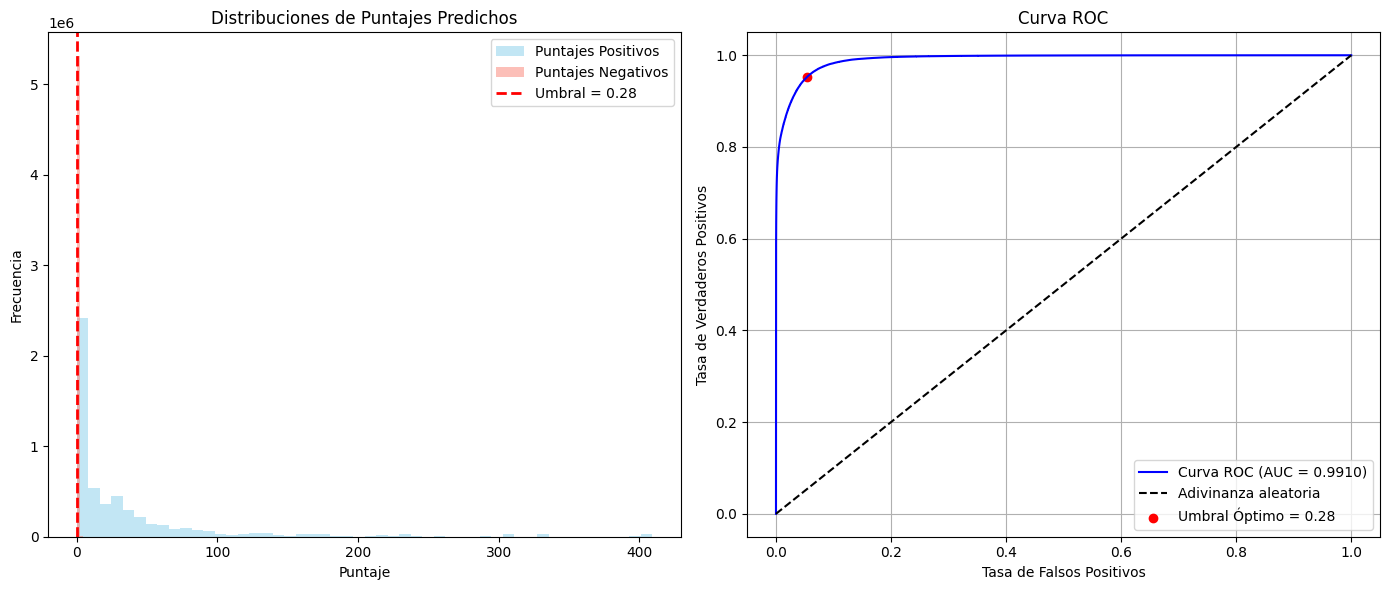
\includegraphics[width=\textwidth]{img/resultados/gnn/partes/caso1_degree/full/roc_GCN_DP_full.png}
        \caption{GCN + Dot Product}
        \label{fig:roc_gcn_dp_full}
    \end{subfigure}
    \hfill
    \begin{subfigure}[b]{0.45\textwidth}
        \centering
        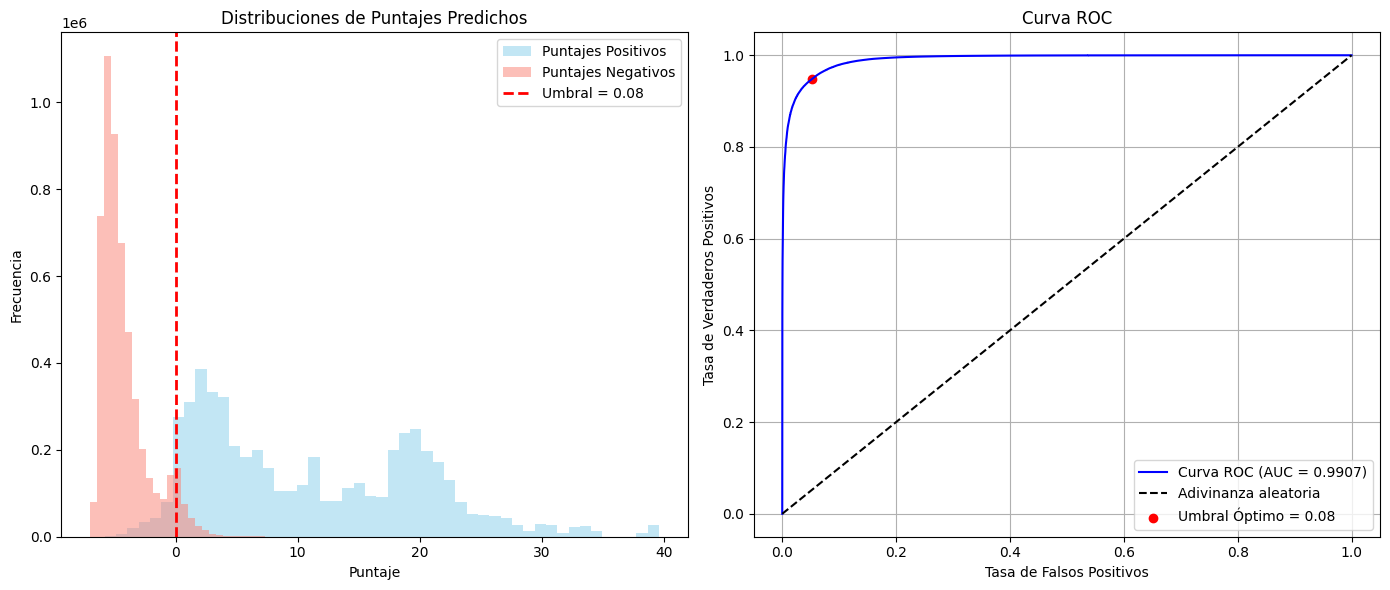
\includegraphics[width=\textwidth]{img/resultados/gnn/partes/caso1_degree/full/roc_GCN_MLP_full.png}
        \caption{GCN + MLP}
        \label{fig:roc_gcn_mlp_full}
    \end{subfigure}

    \vspace{0.5cm}

    % Segunda fila ── GraphSAGE
    \begin{subfigure}[b]{0.45\textwidth}
        \centering
        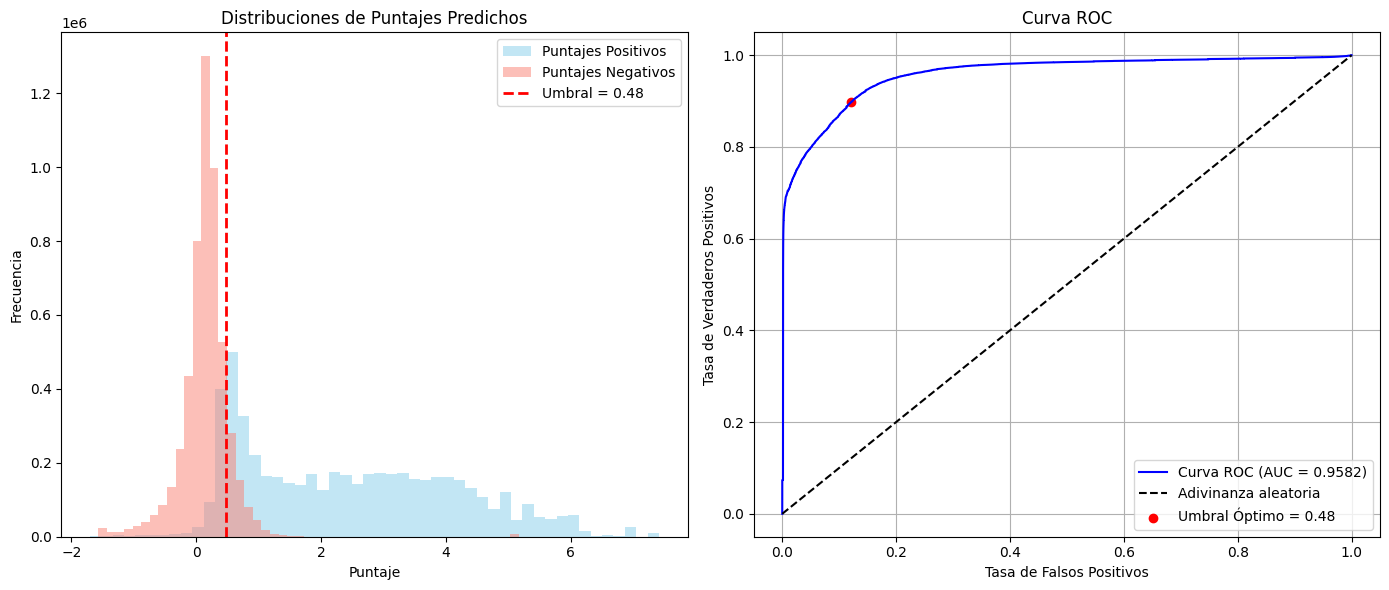
\includegraphics[width=\textwidth]{img/resultados/gnn/partes/caso1_degree/full/roc_GraphSAGE_DP_full.png}
        \caption{GraphSAGE + Dot Product}
        \label{fig:roc_graphsage_dp_full}
    \end{subfigure}
    \hfill
    \begin{subfigure}[b]{0.45\textwidth}
        \centering
        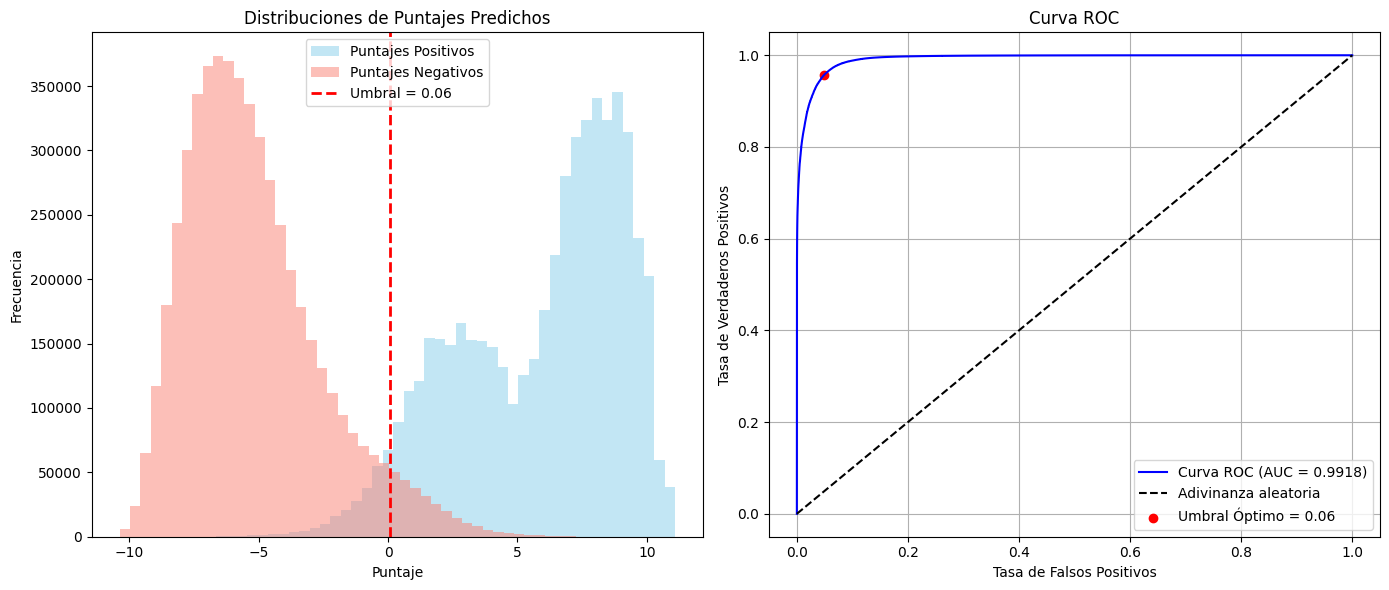
\includegraphics[width=\textwidth]{img/resultados/gnn/partes/caso1_degree/full/roc_GraphSAGE_MLP_full.png}
        \caption{\textbf{GraphSAGE + MLP}}
        \label{fig:roc_graphsage_mlp_full}
    \end{subfigure}

    \vspace{0.5cm}

    % Tercera fila ── GAT
    \begin{subfigure}[b]{0.45\textwidth}
        \centering
        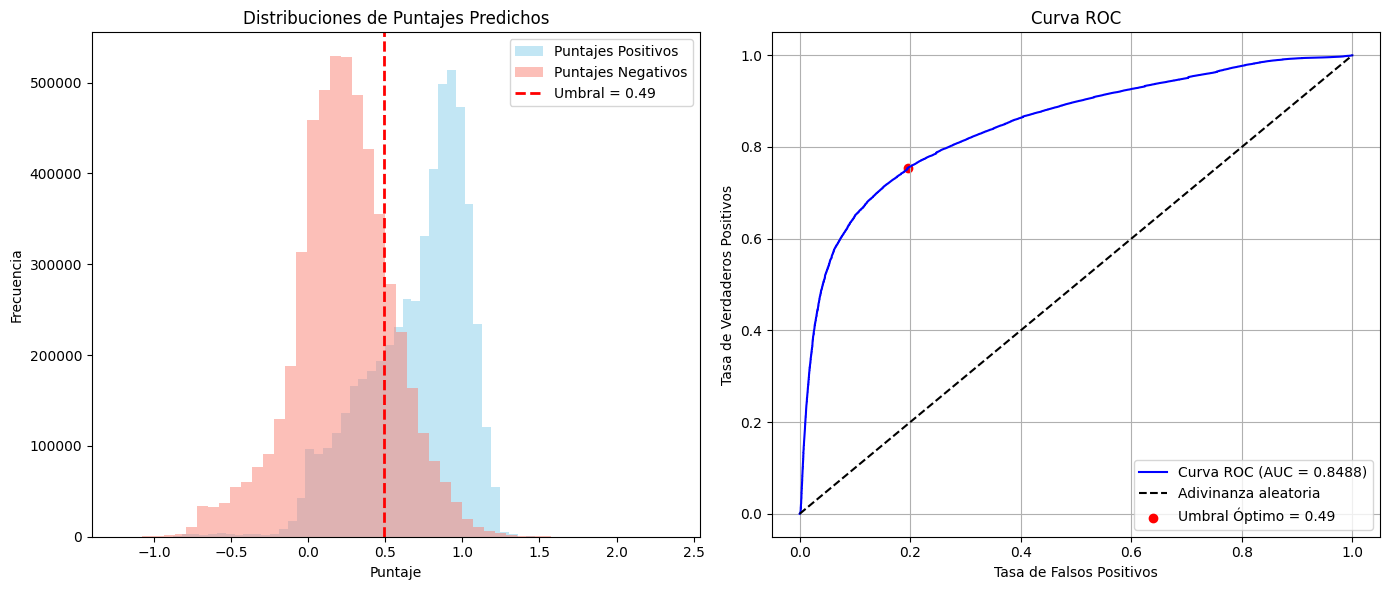
\includegraphics[width=\textwidth]{img/resultados/gnn/partes/caso1_degree/full/roc_GAT_DP_full.png}
        \caption{GAT + Dot Product}
        \label{fig:roc_gat_dp_full}
    \end{subfigure}
    \hfill
    \begin{subfigure}[b]{0.45\textwidth}
        \centering
        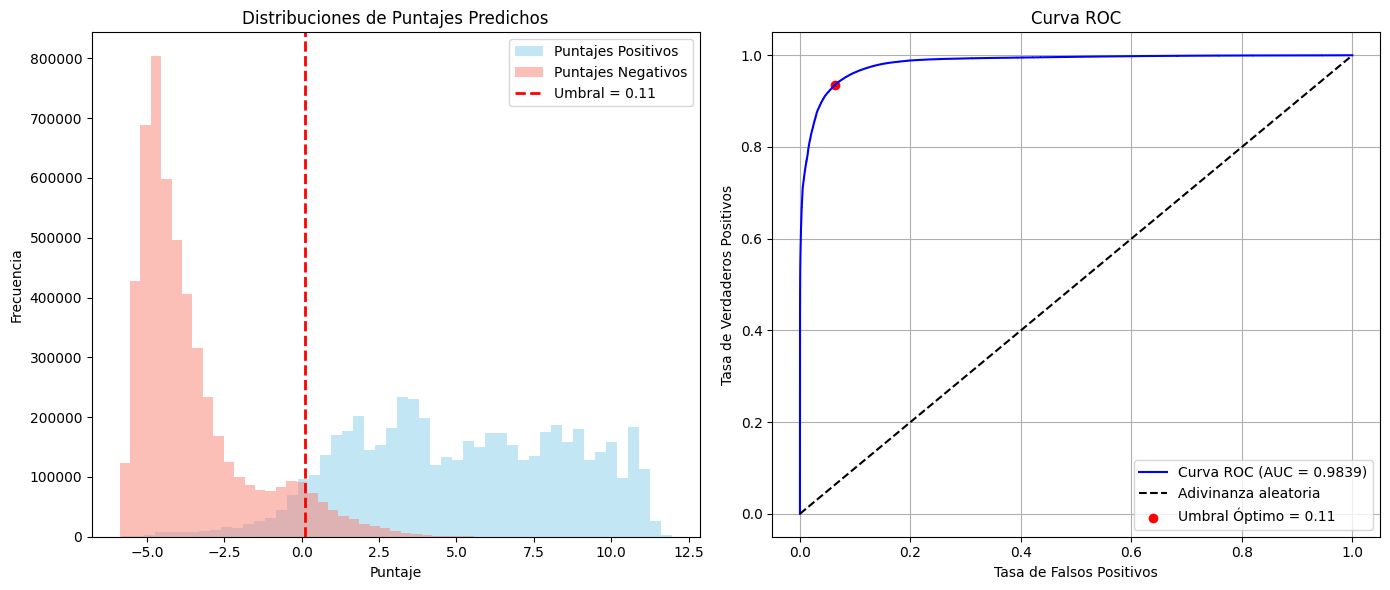
\includegraphics[width=\textwidth]{img/resultados/gnn/partes/caso1_degree/full/roc_GAT_MLP_full.png}
        \caption{GAT + MLP}
        \label{fig:roc_gat_mlp_full}
    \end{subfigure}

    \caption{Curvas ROC y valores AUC para el grafo construido a partir de todas las \texttt{AS\_PATHs}.}
    \label{fig:comparacion_roc_auc_caso1_full}
\end{figure}





\begin{table}[t]
\centering
\begin{tabular}{lccc}
\hline
\textbf{Modelo} & \textbf{Decodificador} & \textbf{AUC}& \textbf{Accuracy(\%)} \\
\hline
GCN & Dot Product & 0.982 & 0.947 \\
GraphSAGE & Dot Product & 0.958 & 0.888 \\
GAT & Dot Product & 0.848 &  0.779 \\
GCN & MLP & 0.990 &  0.948 \\
\textbf{GraphSAGE} & \textbf{MLP} &  \textbf{0.991} & \textbf{0.954} \\
GAT & MLP &  0.983 &  0.936 \\
\hline
\end{tabular}
\caption{Accuracy estimada por combinación de codificador y decodificador.}
\label{tab:accuracy_gnn_full}
\end{table}

\newpage
Podemos observar que el uso de un decoder MLP mejora la capacidad de discriminación entre enlaces positivos y negativos. Se puede ver que en los gráficos donde se usan MLP hay una clara separación entre las clases. 
GraphSAGE con MLP destaca con la mejor combinación (AUC = 0.991, accuracy ≈ 95\%).\\


Luego de la generación de \textit{embeddings}, se evaluó la tarea principal de inferencia de relaciones entre ASes, usando los \textit{embeddings} creados con la tarea previa. En la Tabla~\ref{tab:gnn_resultados_caso1} se muestran los resultados de Precision, Recall y Accuracy obtenidos para cada combinación.\\


\begin{table}[H]
\centering
\resizebox{\textwidth}{!}{
\begin{tabular}{llcccccccccccc}
\toprule
\multirow{2}{*}{\textbf{Modelo}} & 
\multirow{2}{*}{\textbf{Decodificador}} & 
\multicolumn{3}{c}{\textbf{NoBatch-NoW}} & 
\multicolumn{3}{c}{\textbf{NoBatch-W}} & 
\multicolumn{3}{c}{\textbf{Batch-NoW}} & 
\multicolumn{3}{c}{\textbf{Batch-W}} \\
\cmidrule(lr){3-5} \cmidrule(lr){6-8} \cmidrule(lr){9-11} \cmidrule(lr){12-14}
 & & \textbf{Precision} & \textbf{Recall} & \textbf{Accuracy} 
   & \textbf{Precision} & \textbf{Recall} & \textbf{Accuracy} 
   & \textbf{Precision} & \textbf{Recall} & \textbf{Accuracy} 
   & \textbf{Precision} & \textbf{Recall} & \textbf{Accuracy} \\
\midrule
GCN       & Dot Product &74.97&70.91&73.36&71.10&36.84&62.17&74.69&70.72&73.16&63.54&30.52&55.41\\
GraphSAGE & Dot Product &82.99&77.18&80.32&77.56&63.90&72.30&\textbf{82.96}&\textbf{78.88}&\textbf{81.09}&78.71&71.31&75.59\\
GAT       & Dot Product &74.75&70.78&73.15&75.14&39.91&65.74&75.35&71.95&73.99&71.96&49.27&64.41\\
\midrule
GCN       & MLP         &70.06&68.19&69.24&68.80&18.33&48.05&73.17&67.36&71.02&63.76&33.69&55.60\\
GraphSAGE & MLP         &78.92&74.04&76.81&75.94&55.16&69.10&79.70&74.46&77.48&73.01&53.97&66.47\\
GAT       & MLP         &73.93&70.40&72.71&74.33&28.63&62.86&76.42&72.03&74.49&71.43&33.28&59.94\\
\bottomrule
\end{tabular}
}
\caption{Resultados de Precision, Recall y Accuracy (\%) por combinación de encoder y decoder bajo cuatro configuraciones: sin batching y sin balanceo (`NoBatch-NoW'), sin batching con balanceo (`NoBatch-W'), con batching sin balanceo (`Batch-NoW'), y con ambas (`Batch-W'). En negrita se indican los mejores resultados por métrica en cada configuración.}
\label{tab:gnn_resultados_caso1}
\end{table}


Con esto podemos ver que utilizar los atributos provenientes de peeringDB permite obtener mejores resultados que al usar únicamente atributos estructurales básicos como el grado. Asimismo, este caso repite la misma lógica en los resultados donde la MLP es más adecuada como decoder para la tarea auxiliar de link prediction, mientras que Dot Product produce \textit{embeddings} más simples fáciles de analizar para la ANN, lo que resulta en un mejor desempeño en la clasificación final de relaciones entre los Sistemas Autónomos.\\






\subsubsection{Caso 2: Predicción de enlaces utilizando grafo con atributos provenientes de estudios previos}

\begin{itemize}
    \item \textbf{RIBs:} Febrero 2024.
    \item \textbf{Atributos de nodos:} Definidos en un \textit{dataset} utilizado en trabajos anteriores~\cite{BenchmarkingGNN}.
    \item \textbf{Tarea para la creación de \textit{embeddings}:} Determinar la existencia o no de un enlace entre pares de nodos (Sistemas Autónomos).
    \item \textbf{Tamaño \textit{embeddings}:} 32.
    \item \textbf{Epochs:} 100 (GNN) y 20 (ANN).
    \item \textbf{Early Stopping:} Paciencia de 8 epochs.
    \item \textbf{Learning Rate:} 0.001 (GNN) y 0,005 (ANN).
\end{itemize}


Con el objetivo de validar la utilidad de los atributos de nodo definidos en este trabajo, se realizó la inferencia utilizando los atributos propuestos por Giakatos et al.~\cite{BenchmarkingGNN}. Estos atributos fueron extraídos de diferentes fuentes~\cite{PeeringDB,CAIDAAS-rank,BGP2VecCode} y corresponden a la fecha de julio de 2022.  \\

Este grafo, a diferencia del construido en nuestro trabajo, es más pequeño. Esto se debe a que en el estudio de Giakatos et al. se decidió eliminar en tres iteraciones los nodos hoja, es decir, aquellos nodos con grado 1. \\


A continuación, los resultados obtenidos a partir de la tarea para crear \textit{embeddings}. La Tabla~\ref{tab:comparacion_accuracy_caso2_t} resume los valores de AUC y Accuracy alcanzados por cada combinación de encoder y decoder, mientras que la Figura \ref{fig:roc_auc_prev_2022} presenta las curvas ROC asociadas, lo que permite contrastar visualmente el desempeño de cada variante.\\




\begin{figure}[t]
    \centering
    % Primera fila
    \begin{subfigure}[b]{0.45\textwidth}
        \centering
        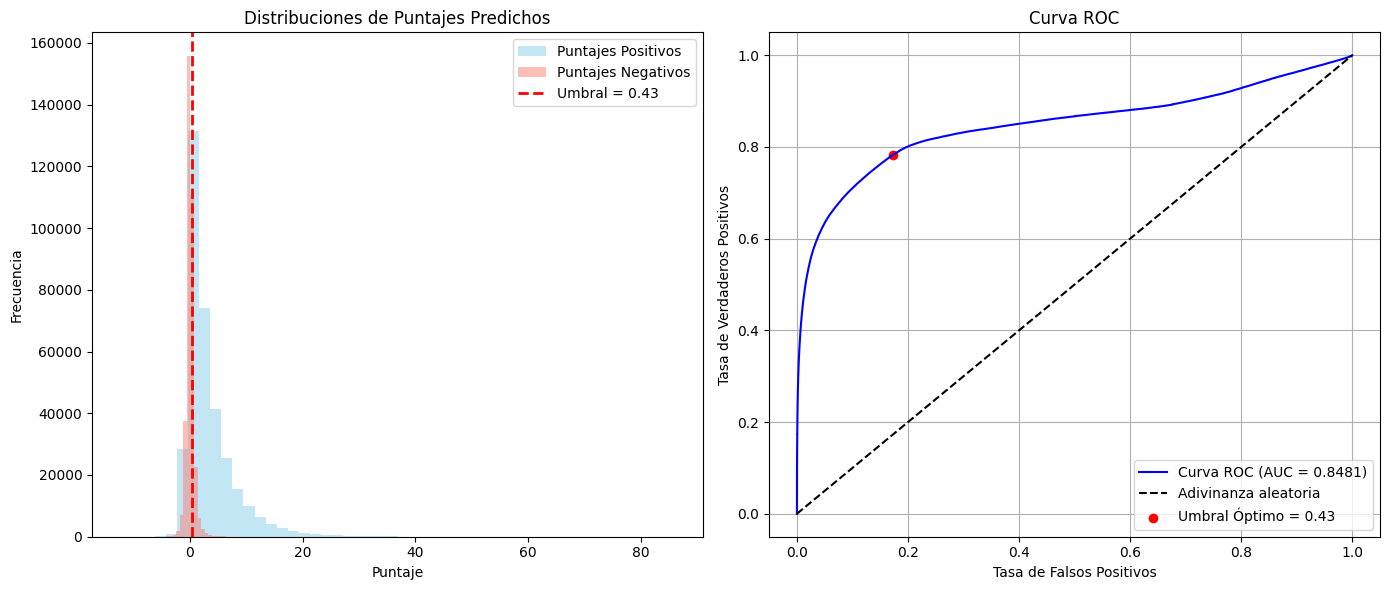
\includegraphics[width=\textwidth]{img//resultados//gnn//partes//caso3_previo/GCN_previo_linkPred.png}
        \caption{GCN + Producto Punto}
    \end{subfigure}
    \hfill
    \begin{subfigure}[b]{0.45\textwidth}
        \centering
        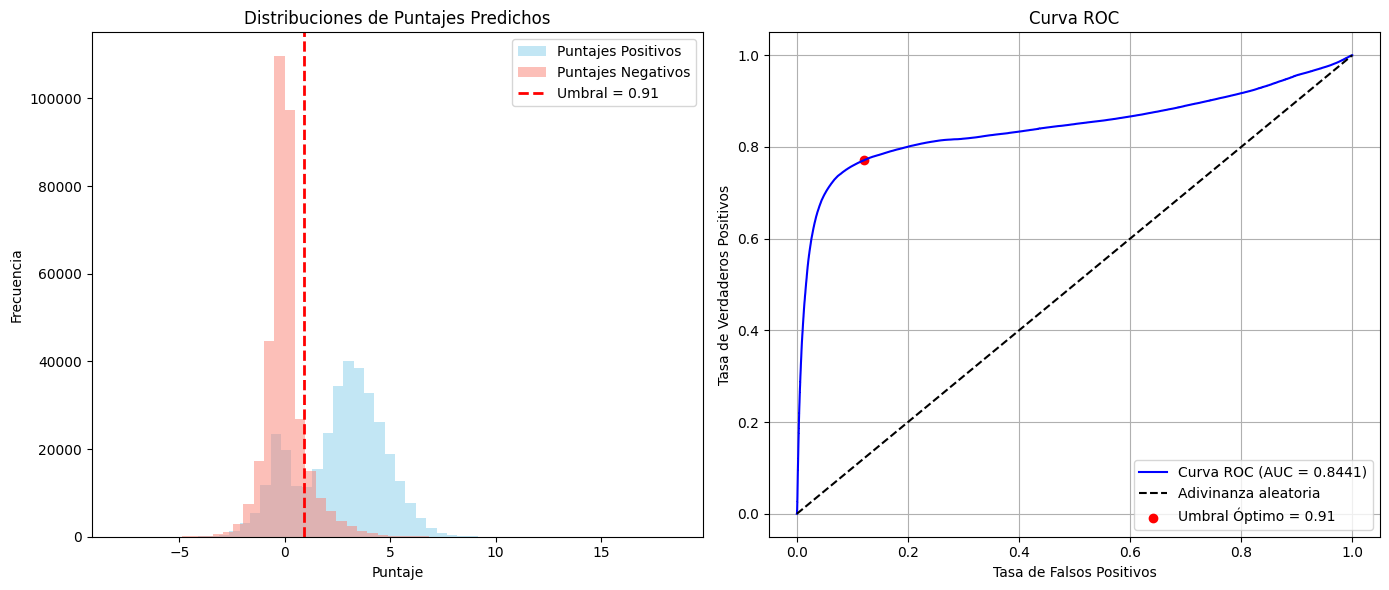
\includegraphics[width=\textwidth]{img//resultados//gnn//partes//caso3_previo/GraphSAGE_previo_LP.png}
        \caption{GraphSAGE + Producto Punto}
        \label{fig:conf_matrix_sage_dp_prev}
    \end{subfigure}

    \vspace{0.5cm}

    % Segunda fila
    \begin{subfigure}[b]{0.45\textwidth}
        \centering
        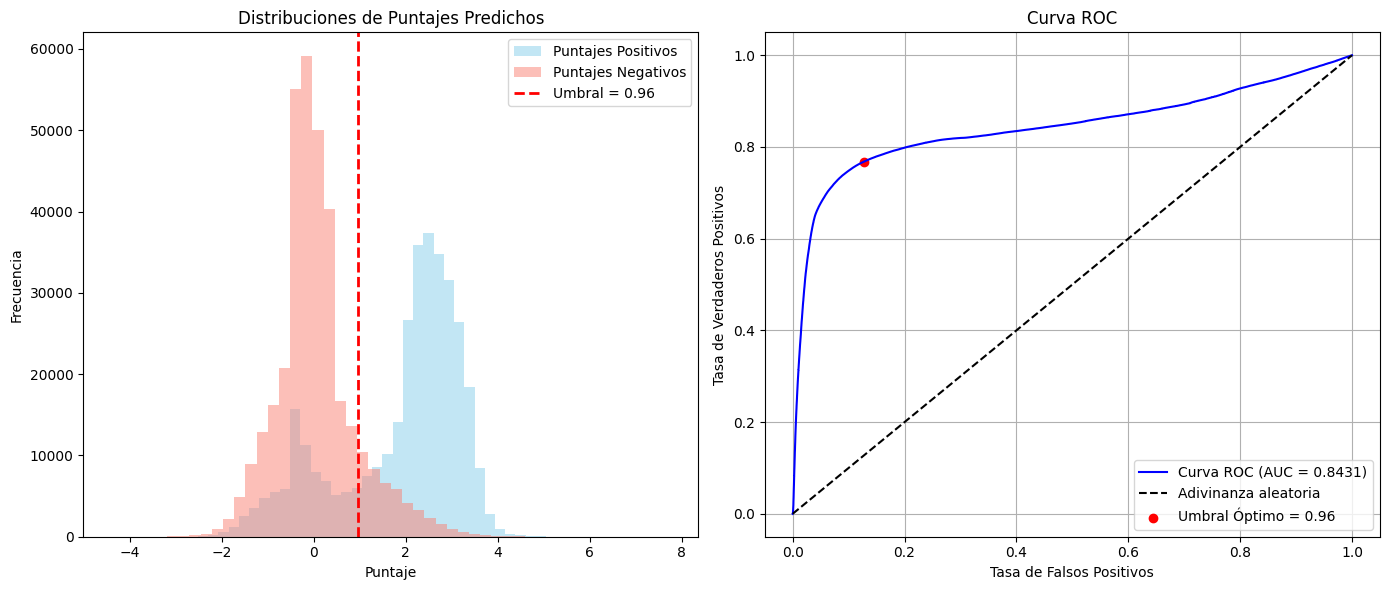
\includegraphics[width=\textwidth]{img//resultados//gnn//partes//caso3_previo/GAT_previo_LP.png}
        \caption{GAT + Producto Punto}
    \end{subfigure}
    \hfill
    \begin{subfigure}[b]{0.45\textwidth}
        \centering
        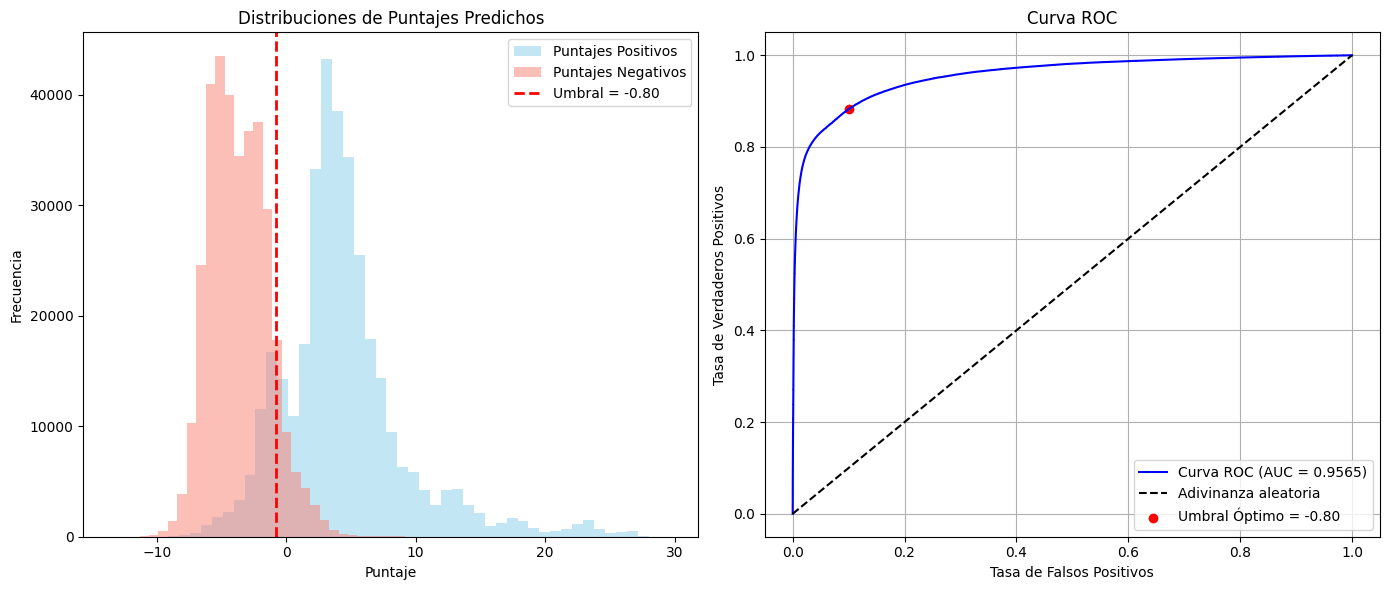
\includegraphics[width=\textwidth]{img//resultados//gnn//partes//caso3_previo/GCN_MLP_previo_LP.png}
        \caption{\textbf{GCN + MLP}}
    \end{subfigure}

    \vspace{0.5cm}

    % Tercera fila
    \begin{subfigure}[b]{0.45\textwidth}
        \centering
        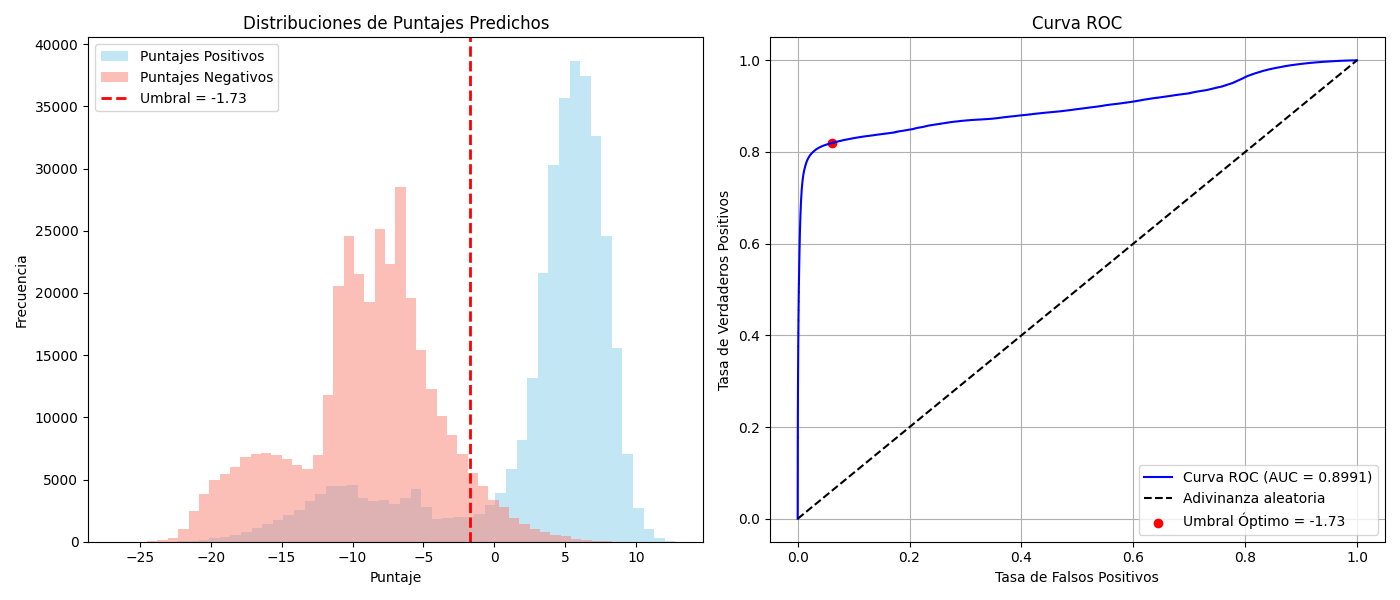
\includegraphics[width=\textwidth]{img/resultados/gnn/partes/caso3_previo/roc_curve_GraphSAGE_MLP.png}
        \caption{GraphSAGE + MLP}
    \end{subfigure}
    \hfill
    \begin{subfigure}[b]{0.45\textwidth}
        \centering
        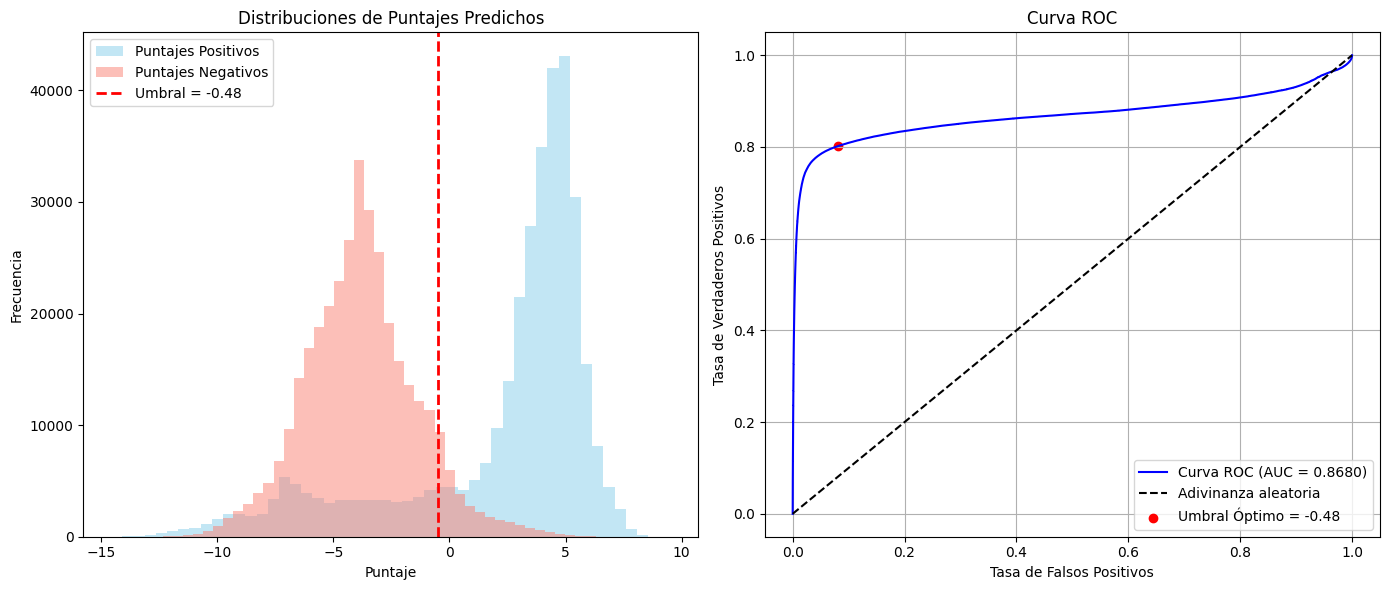
\includegraphics[width=\textwidth]{img//resultados//gnn//partes//caso3_previo/GAT_MLP_previo_LP.png}
        \caption{GAT + MLP}
    \end{subfigure}

    \caption{Curvas ROC y distribución de los resultados. Con diferentes encoders y decoders para grafo con atributos de julio 2022.}
    \label{fig:roc_auc_prev_2022}
\end{figure}



\begin{table}[H]
\centering
\begin{tabular}{lccc}
\hline
\textbf{Modelo} & \textbf{Decodificador} & \textbf{AUC}& \textbf{Accuracy (\%)} \\
\hline
GCN & Dot Product & 0.848  & 0.805 \\
GraphSAGE & Dot Product & 0.844 & 0.825 \\
GAT & Dot Product & 0.843 & 0.820 \\
\textbf{GCN} & \textbf{MLP} & \textbf{0.956} &  \textbf{0.891} \\
GraphSAGE & MLP &  0.937 & 0.874 \\
GAT & MLP & 0.860 & 0.857 \\
\hline
\end{tabular}
\caption{Accuracy de la inferencia con link prediction para la creación de \textit{embeddings}.}
\label{tab:comparacion_accuracy_caso2_t}
\end{table}



Luego de la generación de \textit{embeddings}, se evaluó la tarea principal. En la Tabla~\ref{tab:comparacion_metricas_caso2_now_w} se muestran los resultados obtenidos para cada combinación.\\


\begin{table}[H]
\centering
\resizebox{0.9\textwidth}{!}{
\begin{tabular}{llcccccc}
\toprule
\multirow{2}{*}{\textbf{Modelo}} & 
\multirow{2}{*}{\textbf{Decodificador}} & 
\multicolumn{3}{c}{\textbf{NoBatch-NoW}} & 
\multicolumn{3}{c}{\textbf{NoBatch-W}} \\
\cmidrule(lr){3-5} \cmidrule(lr){6-8}
 & & \textbf{Precision} & \textbf{Recall} & \textbf{Accuracy} 
   & \textbf{Precision} & \textbf{Recall} & \textbf{Accuracy} \\
\midrule
GCN       & Dot Product &82.47&77.02&80.03&80.07&69.73&75.95\\
          & MLP         &79.25&74.73&77.15&73.03&56.64&67.39\\
\midrule
GraphSAGE & Dot Product &\textbf{85.14}&\textbf{82.18}&\textbf{83.76}&79.97&69.27&75.81\\
          & MLP         &75.63&72.60&74.21&68.44&43.77&62.66\\
\midrule
GAT       & Dot Product &84.56&79.89&82.35&78.04&68.46&74.31\\
          & MLP         &77.31&71.85&75.06&65.10&44.02&59.31\\
\bottomrule
\end{tabular}
}
\caption{Resultados de Precision, Recall y Accuracy (\%) por combinación de encoder y decoder bajo dos configuraciones: sin batching y sin balanceo (`NoBatch-NoW'), y sin batching con balanceo (`NoBatch-W'). En negrita se indican los mejores resultados por métrica.}
\label{tab:comparacion_metricas_caso2_now_w}
\end{table}


Para la tarea principal de clasificación de relaciones (C2P, P2P, P2C) se repiten los resultados observados en los Casos 0 y 1: los \textit{embeddings} generados con Dot Product superan en desempeño a los obtenidos con MLP, siendo GraphSAGE + Dot Product la mejor combinación, con una Accuracy ≈ 83.8\% y un Recall ≈ 82.2\%. 
En cuanto al uso de pesos para balancear las clases (P2P mayoritaria), las métricas se reducen de manera significativa. Este experimento genera resultados ligeramente inferiores a los del Caso 0 (Recall ≈ 83\% y Accuracy ≈ 85\%), lo que refuerza la idea de que los atributos diseñados en este trabajo aportan información para distintas tareas en el ámbito de Internet. Esto es porque los atributos del estudio de Giakatos et al.~\cite{BenchmarkingGNN} fueron creados como una base para analizar diferentes tareas exploratorias usando GNNs.\\


%- Con lr 0.05 y sin class wight todas (los 6 casos) predicen p2p
%- Los q ocupan MLP sin class wieght obtienen malos resulatados, tind a predecir como p2p a los p2c y c2p






\subsubsection{Caso 3: Predicción del grado de los nodos utilizando grafo con atributos extraídos de PeeringDB}

\begin{itemize}
    \item \textbf{RIBs:} Febrero 2024.
    \item \textbf{Atributos de nodos:} Dataset creado a partir de PeeringDB.
    \item \textbf{Epochs:} 20.
    \item \textbf{Tarea para la creación de \textit{embeddings}:} Determinar el grado de salida (out-degree) de cada nodo.
    \item \textbf{Tamaño \textit{embeddings}:} 32.
    \item \textbf{Epochs:} 100 (GNN) y 20 (ANN).
    \item \textbf{Early Stopping:} Paciencia de 8 epochs.
    \item \textbf{Learning Rate:} 0.001 (GNN) y 0,001 (ANN).
\end{itemize}

Para este caso, se utilizó la tarea de inferencia del grado de los nodos para la creación de los \textit{embeddings}. Se seleccionó este atributo (grado de salida) debido a que muchas métricas (por ejemplo, el PageRank clásico) se basan principalmente en el grado de salida, ya que representa la cantidad de conexiones que un nodo ofrece hacia otros.\\


%\newpage
%Luego tenemos prediccion del atributo grado, se ocupa el grado de salida porque primero muchos métodos (por ejemplo, PageRank clásico) se basan principalmente en el out-degree, ya que la idea es repartir "importancia" hacia afuera. En nuestro caso el out-degree suele reflejar cuántas conexiones directas ofrece un nodo hacia otros. Por otro lado vimos en lso resultados que generalmente son los mismos nodos que tienne mayor cantidad de in y out degree.\\


Antes del entrenamiento, el grado de los nodos fue calculado y posteriormente se le aplicó una transformación logarítmica, esto porque, como se observó en la Figura~\ref{fig:distribucion_as_grado_salida_entrada_febrero_log}, la distribución del grado de los nodos presenta una alta concentración, donde pocos Sistemas Autónomos poseen un gran número de conexiones y la mayoría tiene pocos. Finalmente, se realizó una normalización para ajustar los valores resultantes al intervalo $[0,1]$, facilitando así el proceso de entrenamiento.\\



\begin{figure}[H]
    \centering
    \begin{subfigure}[b]{0.4\linewidth}
        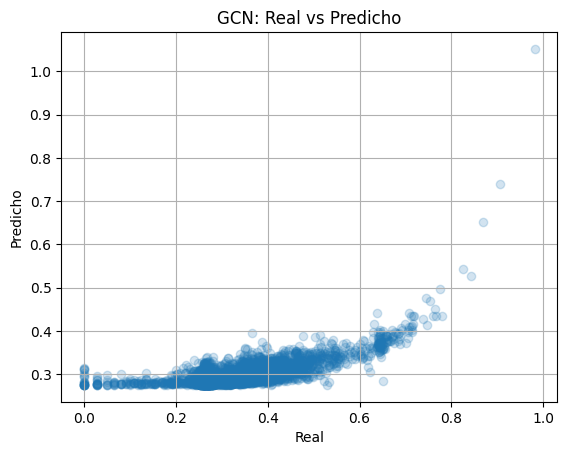
\includegraphics[width=\linewidth]{img//resultados//gnn//partes//caso4_attr_pred//degree/distr_gcn_1m.png}
        \caption{\textbf{GCN}}
        \label{fig:gcn_real_pred}
    \end{subfigure}
    \hfill
    \begin{subfigure}[b]{0.4\linewidth}
        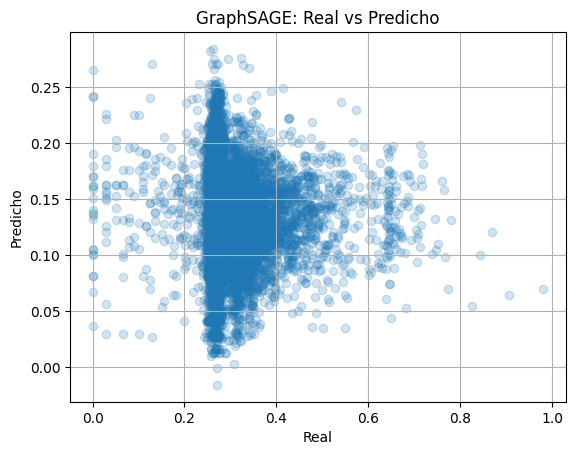
\includegraphics[width=\linewidth]{img//resultados//gnn//partes//caso4_attr_pred//degree/distr_graphsage_1m.png}
        \caption{GraphSAGE}
        \label{fig:graphsage_real_pred}
    \end{subfigure}
    \hfill
    \begin{subfigure}[b]{0.4\linewidth}
        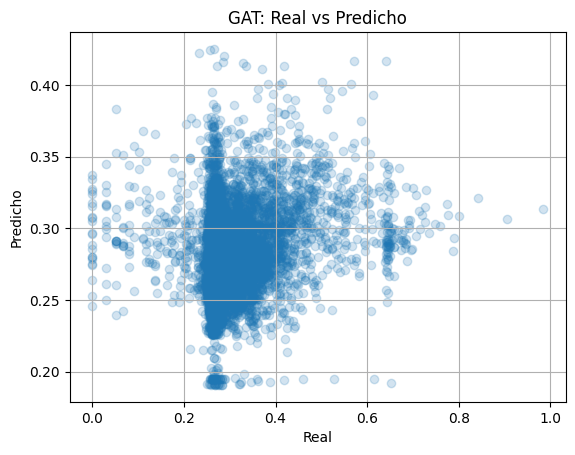
\includegraphics[width=\linewidth]{img//resultados//gnn//partes//caso4_attr_pred//degree/dist_gat_1m.png}
        \caption{GAT}
        \label{fig:gat_real_pred}
    \end{subfigure}
    
    \caption{Comparación entre valores reales y predichos por los modelos GCN, GraphSAGE y GAT.}
    \label{fig:comparacion_real_vs_pred}
\end{figure}

%En la Figura~\ref{fig:comparacion_real_vs_pred} se presenta una comparación entre los valores reales y los predichos por los modelos GCN, GraphSAGE y GAT.\\


La Figura~\ref{fig:gcn_real_pred} muestra los resultados del modelo GCN, donde se observa una tendencia general, aunque el modelo tiende a subestimar los valores. Por otro lado, las Figuras~\ref{fig:graphsage_real_pred} y \ref{fig:gat_real_pred} presentan predicciones concentradas en torno a un valor promedio. Se probaron varios ajustes para intentar solucionar esto, incluyendo cambios en la tasa de aprendizaje, usar una función de pérdida diferente  y aumentar la cantidad de epochs; sin embargo, ninguno de estos ajustes logró una mejora en los resultados. Sugiriendo que GraphSAGE y GAT tienen dificultad para capturar la variabilidad real del grado de salida, es decir, una baja capacidad de generalización.\\



La Tabla~\ref{tab:resultados_regresion_outdegree} muestra las métricas que reflejan el desempeño de cada modelo.\\

\begin{table}[H]
\centering
\caption{Desempeño de arquitecturas GNN para la predicción del atributo \textit{out\_degree} transformado con logaritmo.}
\label{tab:resultados_regresion_outdegree}
\begin{tabular}{lccc}
\toprule
\textbf{Modelo} & \textbf{MAE} & \textbf{MSE} & \textbf{$R^2$} \\
\midrule
GCN        & \textbf{0.0437}  & \textbf{0.00297}  & \textbf{0.1793} \\
GraphSAGE  & 0.0803  & 0.00597  & -1.111 \\
GAT        & 0.0486  & 0.04862  & -0.055  \\
\bottomrule
\end{tabular}
\end{table}



Luego de la generación de \textit{embeddings}, se evaluó la tarea principal. La Tabla~\ref{tab:accuracy_outdegree_downstream} resume los resultados de Precision, Recall y Accuracy.

\begin{table}[H]
\centering
\resizebox{0.7\textwidth}{!}{
\begin{tabular}{lcccccc}
\toprule
\multirow{2}{*}{\textbf{Modelo}} &
\multicolumn{3}{c}{\textbf{NoBatch-NoW}} &
\multicolumn{3}{c}{\textbf{NoBatch-W}} \\
\cmidrule(lr){2-4} \cmidrule(lr){5-7}
 & \textbf{Precision} & \textbf{Recall} & \textbf{Accuracy} 
 & \textbf{Precision} & \textbf{Recall} & \textbf{Accuracy} \\
\midrule
GCN       &67.40&65.52&67.24&62.52&1.39&45.27\\
GraphSAGE &\textbf{84.61}&\textbf{79.65}&\textbf{82.29}& 79.54 & 71.24 & 75.80 \\
GAT       &84.55&76.09&80.70& 78.63 & 67.51 & 73.89 \\
\bottomrule
\end{tabular}
}
\caption{Resultados de Precision, Recall y Accuracy (\%) por modelo GNN bajo dos configuraciones: sin balanceo de clases (`NoBatch-NoW') y con balanceo de clases (`NoBatch-W').}
\label{tab:accuracy_outdegree_downstream}
\end{table}


Con estos resultados podemos ver el impacto de la tarea auxiliar sobre la creación de las representaciones vectoriales de los nodos. Para este caso, si bien GCN obtuvo los mejores resultados en la tarea auxiliar de predicción de grado de salida, sus \textit{embeddings} resultan poco útiles para la clasificación de relaciones entre ASes, 
es decir, no capturan propiedades relevantes para diferenciar relaciones económicas. En cambio, GraphSAGE y GAT, aunque fallan en predecir bien el grado, producen \textit{embeddings} más ricos para la tarea final.\\ 



\subsubsection{Caso 4: Predicción del valor de PageRank utilizando grafo con atributos extraídos de PeeringDB.}

\begin{itemize}
    \item \textbf{RIBs:} Febrero 2024.
    \item \textbf{Atributos de nodos:} Dataset creado a partir de PeeringDB.
    \item \textbf{Epochs:} 100 (GNN) y 20 (ANN).
    \item \textbf{Tarea para la creación de \textit{embeddings}:} Predicción del valor de PageRank de cada nodo, una métrica de centralidad que refleja su importancia en el grafo.
    \item \textbf{Early Stopping:} Paciencia de 8 epochs.
    \item \textbf{Learning Rate:} 0.001 (GNN) y 0,001 (ANN).
\end{itemize}



Primero, se calculó el valor de PageRank para cada nodo, como estos valores tienden a concentrarse en rangos pequeños con algunos valores extremos, se aplicó una transformación logarítmica, con el objetivo de reducir la dispersión y estabilizar la escala. Luego, se normalizó el resultado utilizando una transformación tipo \textit{z-score}.\\







\begin{figure}[H]
    \centering
    % ---------- Fila 1 ----------
    \begin{subfigure}[b]{0.40\linewidth}
        \centering
        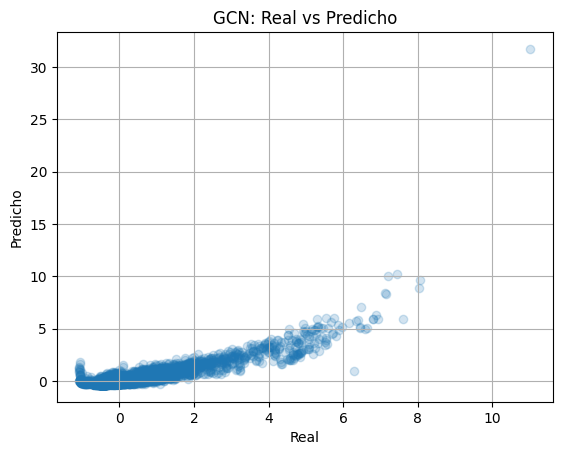
\includegraphics[width=\linewidth]{img//resultados//gnn//partes//caso5/distr_gcn.png}
        \caption{GCN}
        \label{fig:distr_gcn}
    \end{subfigure}
    \hfill
    \begin{subfigure}[b]{0.40\linewidth}
        \centering
        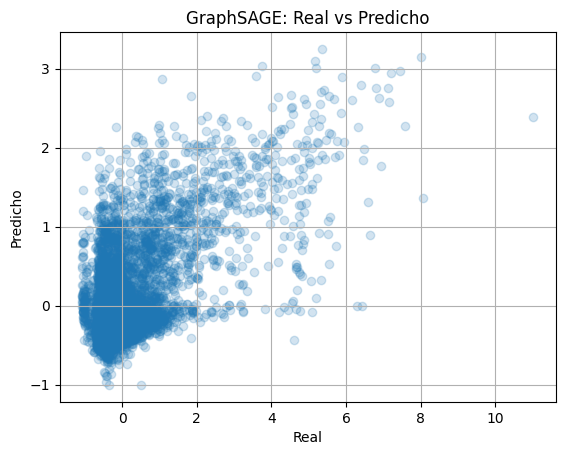
\includegraphics[width=\linewidth]{img//resultados//gnn//partes//caso5/distr_graphsage.png}
        \caption{GraphSAGE}
        \label{fig:distr_graphsage}
    \end{subfigure}

    \vspace{0.8em} % separación vertical entre filas

    % ---------- Fila 2 ----------
    \begin{subfigure}[b]{0.40\linewidth}
        \centering
        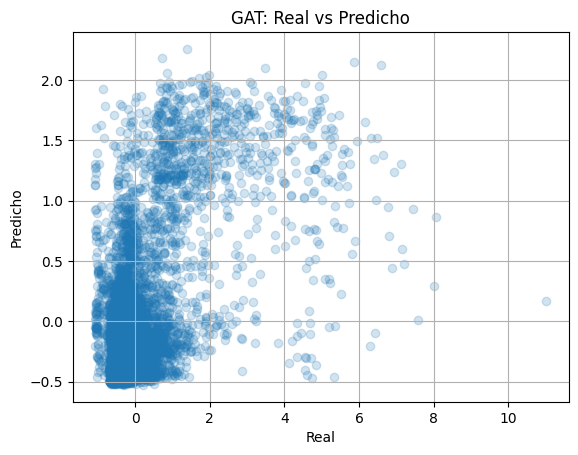
\includegraphics[width=\linewidth]{img//resultados//gnn//partes//caso5/distr_gat.png}
        \caption{GAT}
        \label{fig:distr_gat}
    \end{subfigure}

    \caption{Comparación entre valores reales y predichos por los modelos
GCN, GraphSAGE y GAT.}
    \label{fig:distr_gnn_all}
\end{figure}

La Tabla~\ref{tab:resultados_test_modelos_pagerank} muestra los resultados obtenidos en el conjunto de test para cada arquitectura utilizada.

\begin{table}[H]
\centering
\begin{tabular}{lccc}
\toprule
\textbf{Modelo} & \textbf{MSE} & \textbf{MAE} & \textbf{$R^2$} \\
\midrule
GCN       & \textbf{0.242087} & \textbf{0.316427} & \textbf{0.746798} \\
GraphSAGE & 0.560129 & 0.439433 & 0.414153 \\
GAT       & 0.639733 & 0.463012 & 0.330895 \\
\bottomrule
\end{tabular}
\caption{Resultados para la tarea de predicción de PageRank utilizando distintas arquitecturas GNN. En negrita se resaltan los mejores resultados por métrica.}
\label{tab:resultados_test_modelos_pagerank}
\end{table}



Al igual que en el caso anterior, podemos ver que GCN (Figura~\ref{fig:distr_gcn}) es la que sigue mejor la diagonal, aunque empieza a subestimar los nodos con PageRank más alto. Por otro lado, GraphSAGE y GAT (Figuras~\ref{fig:distr_graphsage} y \ref{fig:distr_gat}) concentran muchos puntos cerca de un valor promedio, lo que indica que les cuesta distinguir los extremos, pero aun así capturan suficiente estructura para la tarea siguiente de inferencia.\\

En cuanto a la tarea \textit{downstream}, la Tabla~\ref{tab:downstream_caso4} muestra los resultados obtenidos en la tarea de inferencia de relaciones a partir de los \textit{embeddings} generados durante la predicción de PageRank. Se presentan los valores de Accuracy tanto para el caso con y sin balance de clases.\\




\begin{table}[H]
\centering
\resizebox{0.7\textwidth}{!}{
\begin{tabular}{lcccccc}
\toprule
\multirow{2}{*}{\textbf{Modelo}} &
\multicolumn{3}{c}{\textbf{NoBatch-NoW}} &
\multicolumn{3}{c}{\textbf{NoBatch-W}} \\
\cmidrule(lr){2-4} \cmidrule(lr){5-7}
 & \textbf{Precision} & \textbf{Recall} & \textbf{Accuracy} 
 & \textbf{Precision} & \textbf{Recall} & \textbf{Accuracy} \\
\midrule
GCN       & 78.55 & 73.04 & 76.29 & 72.16 & 48.21 & 63.30 \\
GraphSAGE & \textbf{86.74} & \textbf{83.58} & \textbf{85.17} & 80.20 & 73.97 & 77.445 \\
GAT       & 84.46 & 79.08 & 81.98 & 80.31 & 71.68 & 76.64 \\
\bottomrule
\end{tabular}
}
\caption{Resultados de Precision, Recall y Accuracy (\%) por modelo GNN bajo dos configuraciones: sin balanceo de clases (`NoBatch-NoW') y con balanceo de clases (`NoBatch-W').}
\label{tab:downstream_caso4}
\end{table}



Aquí se observa que la predicción de PageRank como tarea auxiliar para la creación de embeddings es más apropiada que la predicción de grado para generar \textit{embeddings} de Sistemas Autónomos, donde GCN obtiene el mejor desempeño ($R^2$ ≈ 0.75), mientras que GraphSAGE y GAT muestran un mayor nivel de dispersión y menor poder explicativo. Sin embargo, todos los modelos tienen dificultad  para representar valores extremos, lo que muestra una limitación al trabajar con distribuciones muy desiguales (\textit{long tail}), típicas de la topología de Internet.\\



En comparación con los casos anteriores, este caso, al predecir PageRank, permite generar \textit{embeddings} más informativos que los obtenidos al predecir el grado (Caso 3), capturando mejor la centralidad y relevancia global de los nodos. Sin embargo, los resultados finales son inferiores a los alcanzados por la tarea  de predicción de enlaces (Casos 0, 1 y 2), lo que nos dice que esa tarea es más efectiva para este problema.\\

\newpage
\subsubsection{Caso 5: Creación de \textit{embeddings} a partir de DeepWalk y BGP2Vec}

\begin{itemize}
    \item \textbf{RIBs:} Febrero 2024.
    \item Se aplicó el algoritmo DeepWalk y BGP2Vec para generar una representación vectorial (\textit{embedding}) para cada nodo, basada en recorridos aleatorios.
    \item \textbf{Tarea para la creación de \textit{embeddings}:}
    \item \textbf{Epochs:} 100 (GNN) y 20 (ANN).
    \item \textbf{Early Stopping:} Paciencia de 8 epochs (ANN).
    \item \textbf{Learning Rate:} 0,001 (ANN).
\end{itemize}

La Tabla~\ref{tab:accuracy_gnn_variants_dw_bgp2vc} muestra los resultados obtenidos para la tarea de inferencia a partir de la creación de \textit{embeddings} con los métodos de DeepWalk y BGP2Vec .\\



\begin{figure}[H]
    \centering
    \begin{subfigure}[t]{0.48\textwidth}
        \centering
        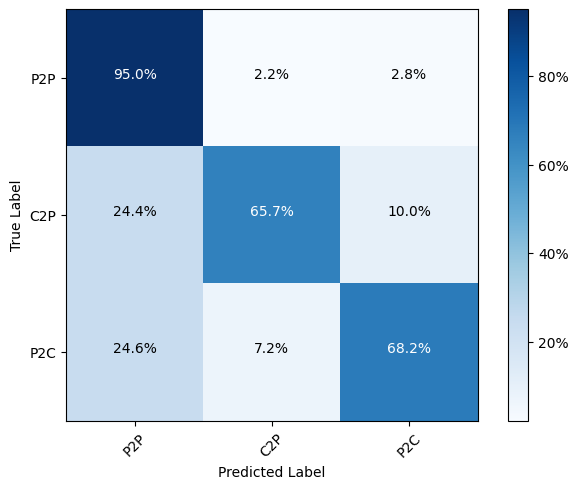
\includegraphics[width=\linewidth]{img//resultados//gnn//partes//caso5/mc_deepwalk_nobatch_noweight.png}
        \caption{DeepWalk}
        \label{fig:mc_deepwalk}
    \end{subfigure}%
    \hfill
    \begin{subfigure}[t]{0.48\textwidth}
        \centering
        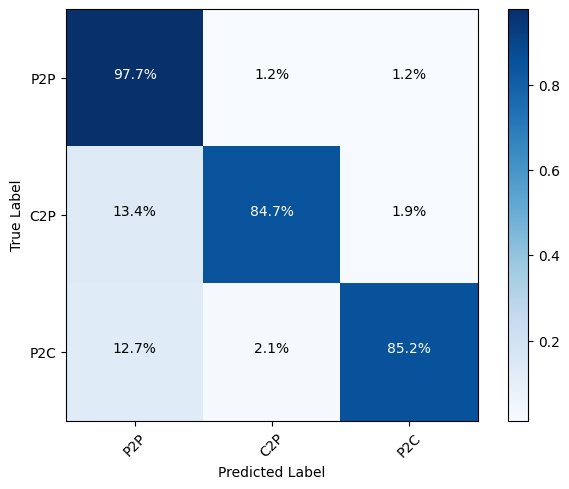
\includegraphics[width=\linewidth]{img//resultados//gnn//partes//caso5/mc_bgp2vec.png}
        \caption{BGP2Vec}
        \label{fig:mc_bgp2vec}
    \end{subfigure}
    \caption{Matrices de confusión obtenidas a partir de los resultados de inferencia utilizando \textit{embeddings} generados con DeepWalk y BGP2Vec.}
    \label{fig:mc_comparacion}
\end{figure}




\begin{table}[H]
\centering
\resizebox{\textwidth}{!}{
\begin{tabular}{lcccccccccccc}
\toprule
\multirow{2}{*}{\textbf{Modelo}} & 
\multicolumn{3}{c}{\textbf{NoBatch-NoW}} & 
\multicolumn{3}{c}{\textbf{NoBatch-W}} & 
\multicolumn{3}{c}{\textbf{Batch-NoW}} & 
\multicolumn{3}{c}{\textbf{Batch-W}} \\
\cmidrule(lr){2-4} \cmidrule(lr){5-7} \cmidrule(lr){8-10} \cmidrule(lr){11-13}
 & \textbf{Precision} & \textbf{Recall} & \textbf{Accuracy} 
 & \textbf{Precision} & \textbf{Recall} & \textbf{Accuracy} 
 & \textbf{Precision} & \textbf{Recall} & \textbf{Accuracy} 
 & \textbf{Precision} & \textbf{Recall} & \textbf{Accuracy} \\
\midrule
DeepWalk  & \textbf{86.99} & \textbf{82.78} & \textbf{84.81} & 84.28 & 81.09 & 82.82 & 87.54 & 85.43 & 86.43 & 84.05 & 81.68 & 82.92 \\
BGP2Vec   & \textbf{94.15} & \textbf{93.72} & \textbf{93.92} & 92.24 & 91.83 & \textbf{92.02} & 94.66 & 94.32 & 94.48 & 92.20 & 91.64 & 91.90 \\
\bottomrule
\end{tabular}
}
\caption{Resultados de Precision, Recall y Accuracy (\%) para la inferencia utilizando \textit{embeddings} generados con DeepWalk y BGP2Vec bajo cuatro configuraciones: sin batching y sin balanceo (`NoBatch-NoW'), sin batching con balanceo (`NoBatch-W'), con batching sin balanceo (`Batch-NoW'), y con ambas (`Batch-W').}
\label{tab:accuracy_gnn_variants_dw_bgp2vc}
\end{table}


%Para estos casos d batching hubo early stoping, en el ccas batch con waight en epochs epoch 9 y en batch sin weigh el 11. =que nos dice eso???

%Poner si os i amtroz bgp 2 vec pues s eve super bacan y si redcococe p2c y c2p , no los pone como p2p2

%Deep walk batchin sin weight tuvo arly stoping en poch 12


%bgp2vec early stoping en 16 con batch y wught



\newpage
Podemos ver que los métodos de generación de \textit{embeddings} basados en recorridos aleatorios, entregan un desempeño superior al de las tareas auxiliares de GNN planteadas en los Casos 0 al 4. DeepWalk alcanza una Accuracy ≈ 85\% (similar a casos anteriores), pero BGP2Vec sobresale con una Accuracy de 92\% y Precision/Recall más equilibrada. Estos resultados sugieren que incorporar información derivada de las rutas BGP permite capturar la estructura y jerarquía de la red, superando a las tareas auxiliares basadas en predicción de enlaces o atributos nodales.\\


%////////////////////////////////////////////////////////////////
\subsection{Resultados de Entrenamiento \textit{End-to-End}} \label{sec:entrenamiento_end_to_end}

En este enfoque, el modelo GNN se entrena directamente para predecir el tipo de relación entre pares de Sistemas Autónomos (ASes), integrando todas las etapas del pipeline en un solo proceso. El flujo de trabajo consistió en los siguientes pasos:
\begin{enumerate}
    \item Importación de los RIBs (Routing Information Base) y construcción del grafo en DGL.
    \item Asociación de atributos a cada nodo del grafo (AS). Se probaron tres tipos de atributos:
    \begin{itemize}
        \item Atributos provistos por el dataset base (extraídos del trabajo de Giakatos et al.~\cite{BenchmarkingGNN}).
        \item Atributos definidos a partir de datos obtenidos de PeeringDB.
        \item Métricas de centralidad computadas directamente desde el grafo (por ejemplo, grado, cercanía, intermediación).
    \end{itemize}
    \item Selección del tipo de GNN y del predictor a utilizar. Como se mencionó en la sección anterior, se exploraron modelos como GraphSAGE y GCN, junto a un MLP como clasificador final.

\end{enumerate}

A diferencia del enfoque anterior, durante el entrenamiento se trabajó con un único grafo, los conjuntos de entrenamiento y test se generan mediante máscaras sobre las aristas, en lugar de crear subgrafos.\\

En cuanto al \textit{split}, ambas aristas dirigidas que conforman un mismo par de AS (src, dst) se asignan al mismo conjunto de datos, de modo que la información de una relación no aparezca simultáneamente en entrenamiento y prueba.\\


A continuación, se presentan los diferentes experimentos creados con este enfoque.\\



\subsubsection{Caso 0: Se utiliza grafo con atributos de nodos extraídos de PeeringDB}

\begin{itemize}
    \item \textbf{RIBs:} Febrero 2024.
    \item \textbf{Atributos de nodos:} Dataset creado a partir de PeeringDB.
    \item \textbf{Epochs:} 100.
    \item \textbf{Early Stopping:} Paciencia de 8 epochs.
    \item \textbf{Learning Rate:} de 0,02.
\end{itemize}

Se entrena el modelo sobre la tarea específica de clasificación de aristas para saber la relación económica que dos Sistemas Autónomos comparten. Este primer caso utiliza los atributos creados a partir de PeeringDB.\\

% El grafo construido utilizado para este enfoque cuenta con un total de 401.308 nodos y 1.676.600 aristas dirigidas. Cada nodo posee un vector de atributos de dimensión 68. En cuanto a las aristas, se asignaron etiquetas económicas según el dataset de CAIDA: un total de 977.554 aristas fueron etiquetadas, mientras que 699.046 no poseen etiqueta.\\


% La distribución de clases fue la siguiente:
% \begin{itemize}
%     \item \texttt{C2P}: 668.732 aristas
%     \item \texttt{P2C}: 154.411 aristas
%     \item \texttt{P2P}: 154.411 aristas
%     \item Sin etiqueta: 699.046 aristas (marcadas como $-1$)
% \end{itemize}



\begin{table}[H]
\centering
\caption{Resultados de clasificación por modelo utilizando decodificadores Bilinear y MLP.}
\label{tab:resultados_caso0_bilinear_mlp_500ep}
\resizebox{\textwidth}{!}{
\begin{tabular}{llccc}
\toprule
\textbf{Modelo} & \textbf{Decoder} & \textbf{Precision (\%)} & \textbf{Recall (\%)} & \textbf{Accuracy (\%)} \\
\midrule
GCN       & Bilinear & 88.26 & 85.90 &  91.01 \\
GraphSAGE & Bilinear & 90.53 & 87.78 & 92.57 \\
GAT       & Bilinear & 85.19 & 86.25 & 90.56 \\
\midrule
GCN       & MLP      & 87.74 & 82.00 & 89.41 \\
GraphSAGE & MLP      & \textbf{91.06} & \textbf{89.85} & \textbf{93.48} \\
GAT       & MLP      & 89.44 & 85.22 & 91.57 \\
\bottomrule
\end{tabular}
}
\end{table} 





Como se muestra en la Tabla~\ref{tab:resultados_caso0_bilinear_mlp_500ep}, GraphSAGE alcanza el mejor desempeño general, con un 93,48\% de \textit{Accuracy} al igual que en Precision y Recall.\\

\begin{figure}[H]
    \centering

    \begin{minipage}[b]{0.32\linewidth}
        \centering
        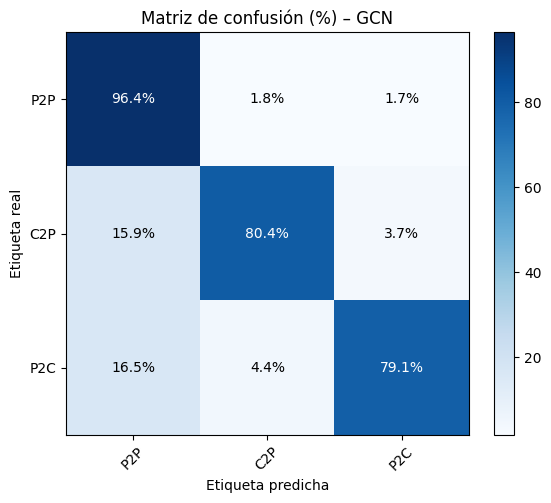
\includegraphics[width=\linewidth]{img//resultados//gnn//end-to-end//caso0/mc_gcn_caso0_b.png}
%        \caption{Matriz de confusión – GCN}
        \label{fig:mc_gcn_caso0}
    \end{minipage}
    \hfill
    \begin{minipage}[b]{0.32\linewidth}
        \centering
        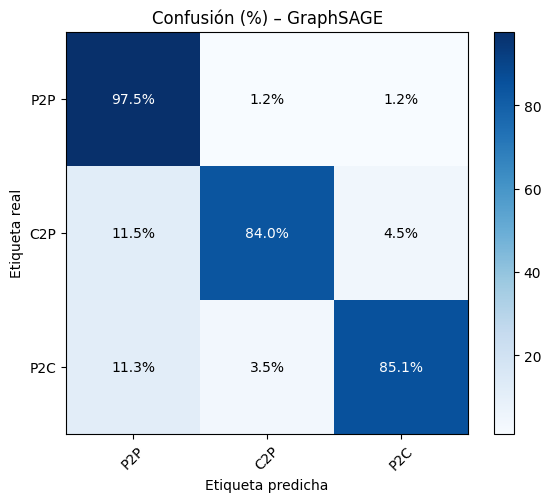
\includegraphics[width=\linewidth]{img//resultados//gnn//end-to-end//caso0/mc_graphsage_mlp_caso0.png}
%        \caption{Matriz de confusión – GraphSAGE}
        \label{fig:mc_graphsage_caso0}
    \end{minipage}
    \hfill
    \begin{minipage}[b]{0.32\linewidth}
        \centering
        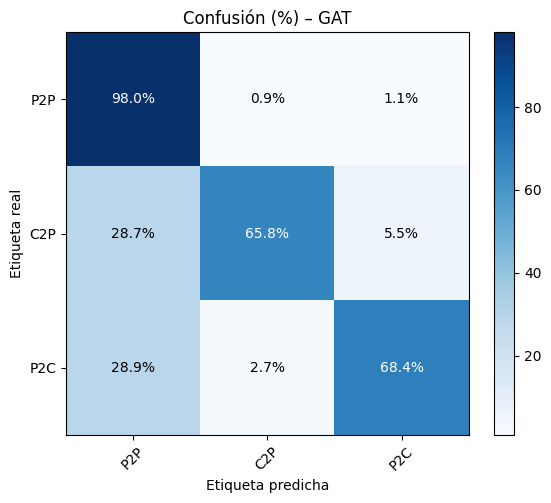
\includegraphics[width=\linewidth]{img//resultados//gnn//end-to-end//caso0/mc_gat_mlp_caso0.png}
%        \caption{Matriz de confusión – GAT}
        \label{fig:mc_gat_caso0}
    \end{minipage}
    \caption{Matrices de confusión obtenidas para el Caso 0 utilizando diferentes modelos GNN (GCN, GraphSAGE y GAT) con decodificador Bilinear.}

\end{figure}





\begin{figure}[H]
    \centering

    \begin{minipage}[b]{0.32\linewidth}
        \centering
        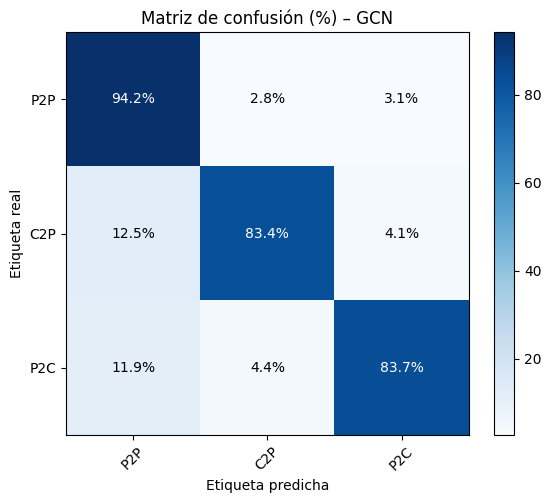
\includegraphics[width=\linewidth]{img//resultados//gnn//end-to-end//caso0/mc_gcn_mlp_caso0.png}
        % \caption{Matriz de confusión – GCN con MLP Early stop en epoch 110}
        \label{fig:mc_gcn_mlp_caso0}
    \end{minipage}
    \hfill
    \begin{minipage}[b]{0.32\linewidth}
        \centering
        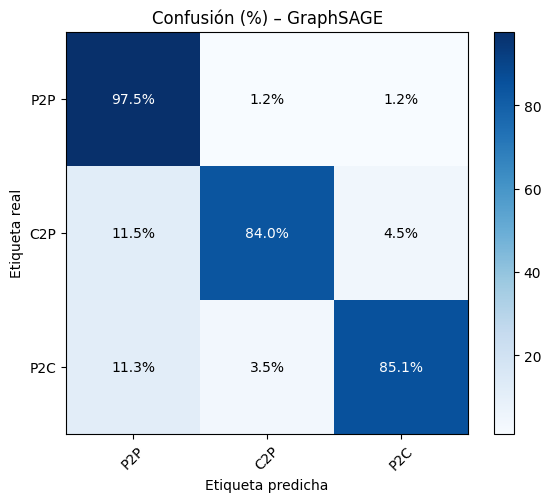
\includegraphics[width=\linewidth]{img//resultados//gnn//end-to-end//caso0/mc_graphsage_mlp_caso0.png}
        % \caption{Matriz de confusión – GraphSAGE con MLP Early stop en epoch 325}
        \label{fig:mc_graphsage_mlp_caso0}
    \end{minipage}
    \hfill
    \begin{minipage}[b]{0.32\linewidth}
        \centering
        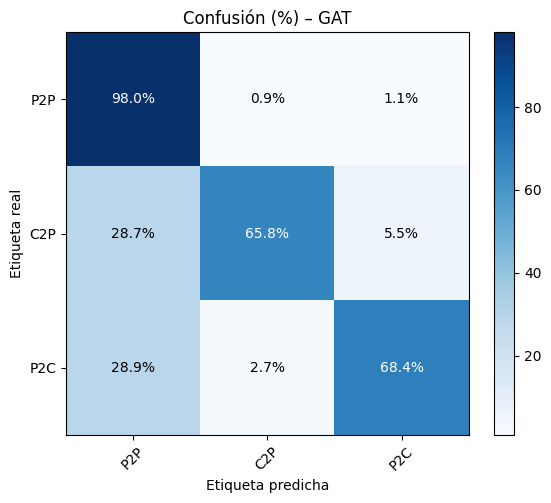
\includegraphics[width=\linewidth]{img//resultados//gnn//end-to-end//caso0/mc_gat_mlp_caso0.png}
        % \caption{Matriz de confusión – GAT con MLP Early stop en epoch 123}
        \label{fig:mc_gat_mlp_caso0}
    \end{minipage}
    \caption{Matrices de confusión obtenidas para el Caso 0 utilizando diferentes modelos GNN (GCN, GraphSAGE y GAT) con decodificador MLP.}

\end{figure}

Con este caso del enfoque \textit{end-to-end} podemos ver una clara mejora respecto al enfoque \textit{por etapas}. Las GNNs directamente sobre la tarea final (clasificación de relaciones económicas) permiten obtener representaciones de nodos más ajustadas al problema. La arquitectura GraphSAGE con decodificador MLP alcanza el mejor desempeño, con un Accuracy de 93,48\%, Precision 91\% y Recall 90\%.\\



% Para ver si lo sbuenos rusltados s trataban por los attributos se corrio l xprimnto 5 , donde se diron attr alatorios a cada nodo y lugo s ntrno.\\



\subsubsection{Caso 1: Se utiliza grafo con atributos de grado de entrada y salida}

\begin{itemize}
    \item \textbf{RIBs:} Febrero 2024.
    \item \textbf{Atributos de nodos:} Grado de entrada y salida de cada nodo.
    \item \textbf{Epochs:} 100.
    \item \textbf{Early Stopping:} Paciencia de 8 epochs.
    \item \textbf{Learning Rate:} 0,01.
\end{itemize}


Se entrena el modelo utilizando únicamente el decoder MLP, decisión que se tomó luego de ver los resultados obtenidos en el Caso 0, donde este alcanzó el mejor desempeño. A diferencia del caso anterior, se utilizan como atributos de los nodos solo el grado de entrada y el grado de salida de cada Sistema Autónomo.\\


\begin{figure}[H]
    \centering

    \begin{minipage}[b]{0.32\textwidth}
        \centering
        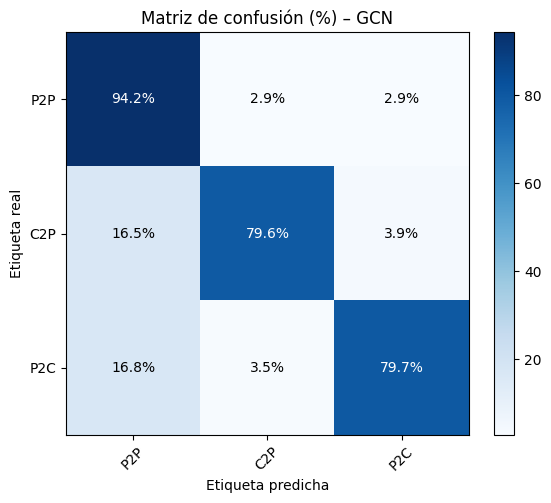
\includegraphics[width=\linewidth]{img//resultados//gnn//end-to-end//caso2/mc_bi_gcn.png}
%        \caption{GCN con decodificador bilineal}
        \label{fig:mc_bi_gcn}
    \end{minipage}
    \hfill
    \begin{minipage}[b]{0.32\textwidth}
        \centering
        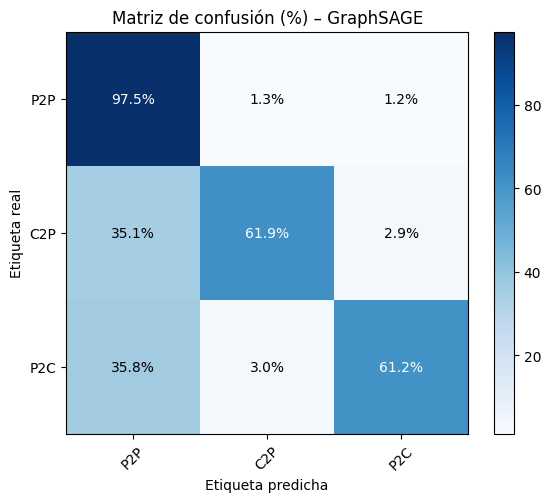
\includegraphics[width=\linewidth]{img//resultados//gnn//end-to-end//caso2/mc_bi_graphsage.png}
 %       \caption{GraphSAGE con decodificador bilineal}
        \label{fig:mc_bi_graphsage}
    \end{minipage}
    \hfill
    \begin{minipage}[b]{0.32\textwidth}
        \centering
        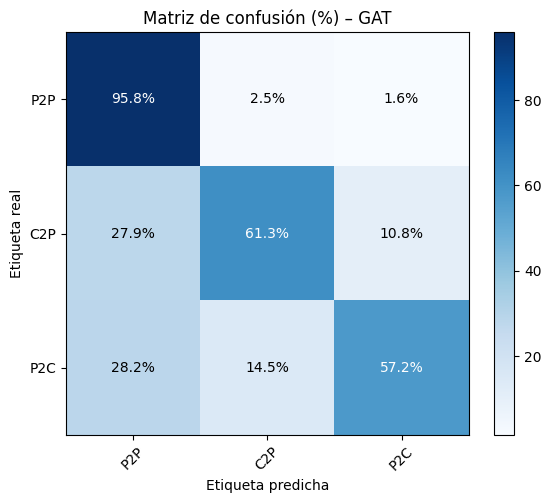
\includegraphics[width=\linewidth]{img//resultados//gnn//end-to-end//caso2/mc_bi_gat.png}
 %       \caption{GAT con decodificador bilineal}
        \label{fig:mc_bi_gat}
    \end{minipage}
    \caption{Matrices de confusión obtenidas para el Caso 1 utilizando diferentes modelos GNN (GCN, GraphSAGE y GAT) con decodificador MLP.}
\end{figure}




\begin{table}[H]
\centering
\begin{tabular}{lcccc}
\toprule
\textbf{Modelo} & \textbf{Precision (\%)}  & \textbf{Recall (\%)}  & \textbf{Accuracy (\%)} \\
\midrule
GCN        & \textbf{85.90} & \textbf{82.82} & \textbf{89.01} \\
GraphSAGE  & 84.76 & 67.92 & 83.44 \\
GAT        & 73.97 & 72.53 & 82.70 \\
\bottomrule
\end{tabular}
\caption{Resultados de clasificación por modelo utilizando decodificador MLP.}
\label{tab:caso1_mlp}
\end{table}




A pesar de utilizar atributos básicos como el grado de entrada y salida, este enfoque logra resultados competitivos, donde se alcanza un 89\% de Accuracy. Sin embargo, el resultado es inferior al caso 0 donde se trabaja con los atributos obtenidos de PeeringDB, lo que confirma que la calidad de los atributos  nodales es importante para obtener resultados superiores en la inferencia de relaciones económicas entre ASes. 




\subsubsection{Caso 2: Enfoque \textit{end-to-end} utilizando grafo con atributos de PeeringDB y muestreo aleatorio de vecinos (Random Neighbour Sampling)}

\begin{itemize}
    \item \textbf{RIBs:} Febrero 2024.
    \item \textbf{Atributos de nodos:} Dataset creado a partir de PeeringDB.
    \item \textbf{Esquema de entrenamiento:} Por \textit{batches}, aplicando \textit{Random Neighbour Sampling} en cada capa.
    \item \textbf{Epochs:}  100
    \item \textbf{Configuraciones evaluadas:} 5, 10, 15 y 20 vecinos por capa.
    \item \textbf{Early stopping:} Paciencia de 8 epochs.
    \item \textbf{Learning rate:} 0,01.
\end{itemize}








\begin{table}[H]
\centering
\caption{Desempeño de arquitecturas GNN con diferentes cantidades de vecinos aleatorios por capa.}
\label{tab:resultados_random_neighbors_resumen}
\resizebox{0.85\textwidth}{!}{
\begin{tabular}{lccccc}
\toprule
\textbf{Modelo} & \textbf{Vecinos} & \textbf{Precision (\%)} & \textbf{Recall (\%)} & \textbf{Accuracy (\%)} \\
\midrule
GCN        & 5  & 81.09 & 66.65 & 82.26 \\
GraphSAGE  & 5  & 81.55 & 58.95 & 79.68 \\
GAT        & 5  & 75.31 & 68.74 & 81.33 \\
\midrule
GCN        & 10 & 88.84 & 76.85 & 88.17 \\
GraphSAGE  & 10 & 87.60 & 80.94 & 89.38 \\
GAT        & 10 & 86.41 & 81.88 & 89.24 \\
\midrule
GCN        & 15 & 90.57 & 80.89 & 90.12 \\
GraphSAGE  & 15 & 90.90 & 81.89 & 90.56 \\
GAT        & 15 & 89.29 & 82.41 & 90.39 \\
\midrule
GCN        & 20 & \textbf{90.85} & \textbf{86.25} & \textbf{92.18} \\
GraphSAGE  & 20 & 90.46 & 85.35 & 91.78 \\
GAT        & 20 & 90.57 & 85.44 & 91.78 \\
\bottomrule
\end{tabular}
}
\end{table}

% ------------------------------------------
\begin{figure}[H]
    \centering

    \begin{minipage}[b]{0.32\textwidth}
        \centering
        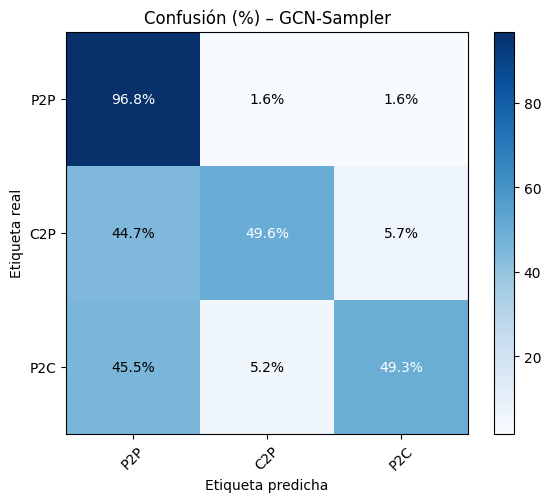
\includegraphics[width=\linewidth]{img//resultados//gnn//end-to-end//caso3/mc_gcn_mlp.png}
        % \caption{GCN con decoder MLP (5 vecinos)}
        \label{fig:mc_gcn_mlp_5nei}
    \end{minipage}
    \hfill
    \begin{minipage}[b]{0.32\textwidth}
        \centering
        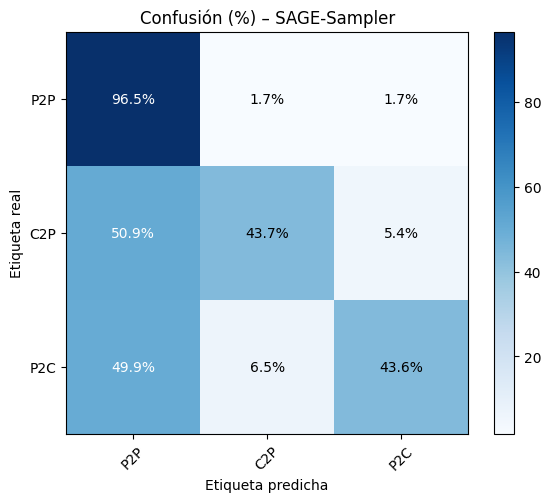
\includegraphics[width=\linewidth]{img//resultados//gnn//end-to-end//caso3/mc_graphsage_mlp.png}
        % \caption{GraphSAGE con decoder MLP (5 vecinos)}
        \label{fig:mc_graphsage_mlp_5nei}
    \end{minipage}
    \hfill
    \begin{minipage}[b]{0.32\textwidth}
        \centering
        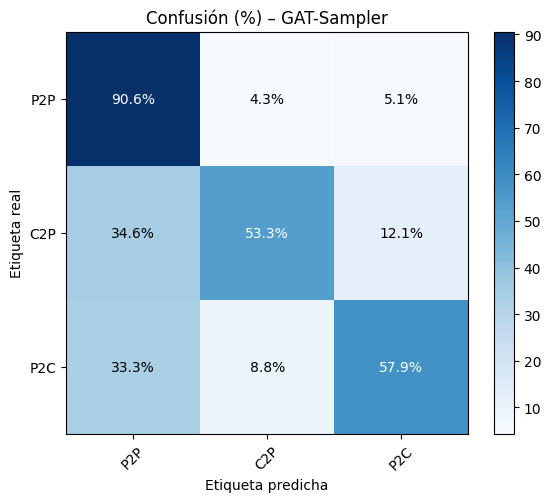
\includegraphics[width=\linewidth]{img//resultados//gnn//end-to-end//caso3/mc_gat_mlp.png}
        % \caption{GAT con decoder MLP (5 vecinos)}
        \label{fig:mc_gat_mlp_5nei}
    \end{minipage}
    \caption{Matrices de confusión obtenidas utilizando diferentes modelos GNN (GCN, GraphSAGE y GAT) con decodificador MLP y muestreo aleatorio de 5 vecinos por capa. }

 \end{figure}

% ------------------------------------------
\begin{figure}[H]
    \centering

    \begin{minipage}[b]{0.32\textwidth}
        \centering
        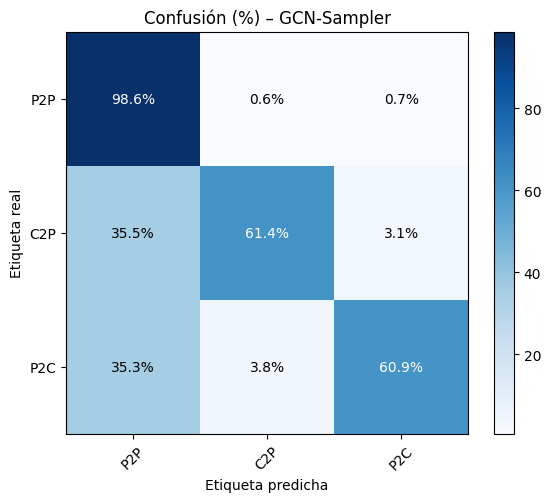
\includegraphics[width=\linewidth]{img//resultados//gnn//end-to-end//caso3/mc_gcn_mlp_10nei.png}
        %\caption*{(a) GCN con decoder MLP — Early stopping en epoch 15}        
        \label{fig:mc_gcn_mlp_10nei}
    \end{minipage}
    \hfill
    \begin{minipage}[b]{0.32\textwidth}
        \centering
        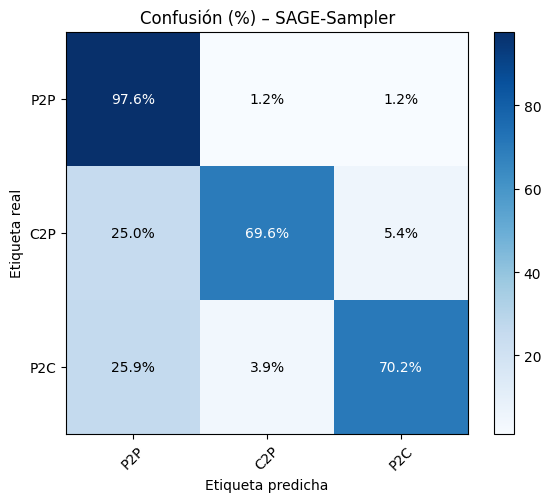
\includegraphics[width=\linewidth]{img//resultados//gnn//end-to-end//caso3/mc_graghsage_mlp_10nei.png}
       %\caption*{(b) GraphSAGE con decoder MLP — Early stopping en epoch 23}        
        \label{fig:mc_graphsage_mlp_10nei}
    \end{minipage}
    \hfill
    \begin{minipage}[b]{0.32\textwidth}
        \centering
        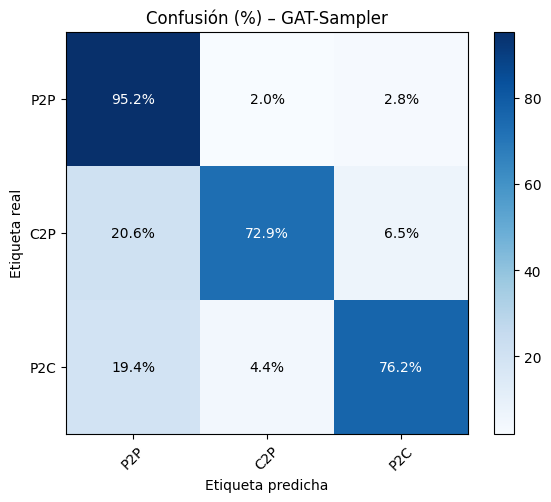
\includegraphics[width=\linewidth]{img//resultados//gnn//end-to-end//caso3/mc_gat_mlp_10nei.png}
        %\caption*{(c) GAT con decoder MLP — Early stopping en epoch 38}  
        \label{fig:mc_gat_mlp_10nei}
    \end{minipage}
    
    \caption{Matrices de confusión obtenidas utilizando diferentes modelos GNN (GCN, GraphSAGE y GAT) con decodificador MLP y muestreo aleatorio de 10 vecinos por capa. }
\end{figure}
% ------------------------------------------

\begin{figure}[H]
    \centering

    \begin{minipage}[b]{0.32\textwidth}
        \centering
        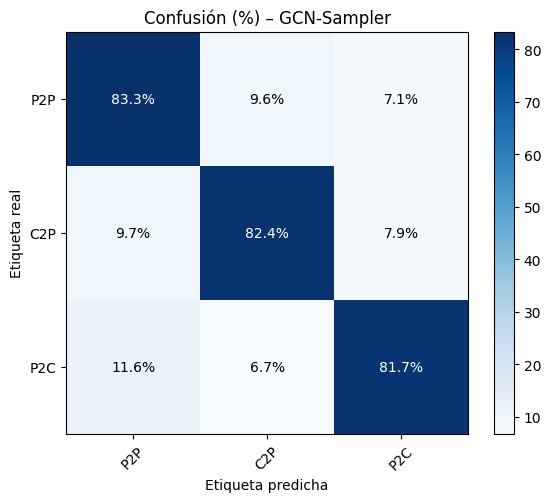
\includegraphics[width=\linewidth]{img//resultados//gnn//end-to-end//caso3/mc_gcn_mlp_15nei.png}
        % \caption{GCN con decoder MLP (15 vecinos)}
        \label{fig:mc_gcn_mlp_15nei}
    \end{minipage}
    \hfill
    \begin{minipage}[b]{0.32\textwidth}
        \centering
        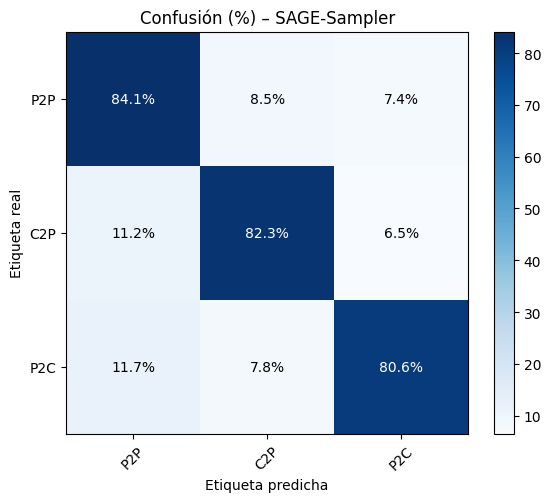
\includegraphics[width=\linewidth]{img//resultados//gnn//end-to-end//caso3/mc_graphsage_mlp_15nei.png}
        % \caption{GraphSAGE con decoder MLP (15 vecinos)}
        \label{fig:mc_graphsage_mlp_15nei}
    \end{minipage}
    \hfill
    \begin{minipage}[b]{0.32\textwidth}
        \centering
        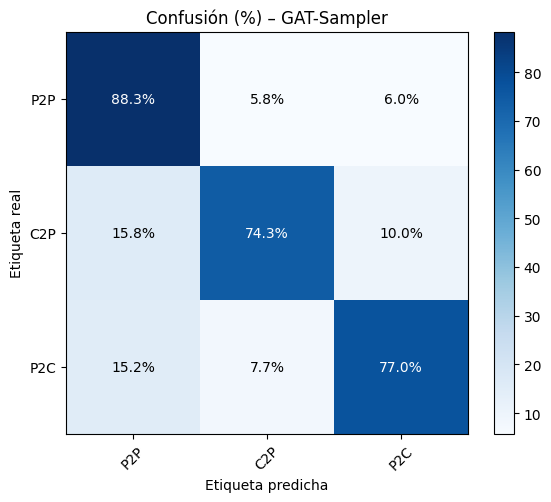
\includegraphics[width=\linewidth]{img//resultados//gnn//end-to-end//caso3/mc_gat_mlp_15nei.png}
        % \caption{GAT con decoder MLP (15 vecinos)}
        \label{fig:mc_gat_mlp_15nei}
    \end{minipage}
    \caption{Matrices de confusión obtenidas utilizando diferentes modelos GNN (GCN, GraphSAGE y GAT) con decodificador MLP y muestreo aleatorio de 15 vecinos por capa. }
\end{figure}

% ------------------------------------------

\begin{figure}[H]
    \centering

    \begin{minipage}[b]{0.32\linewidth}
        \centering
        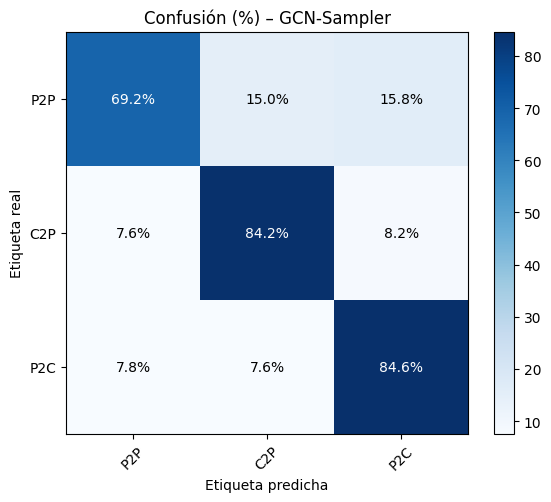
\includegraphics[width=\linewidth]{img//resultados//gnn//end-to-end//caso3/mc_gcn_mlp_20nei.png}
        % \caption*{GCN + MLP}
        \label{fig:mc_gcn_mlp_20nei}
    \end{minipage}
    \hfill
    \begin{minipage}[b]{0.32\linewidth}
        \centering
        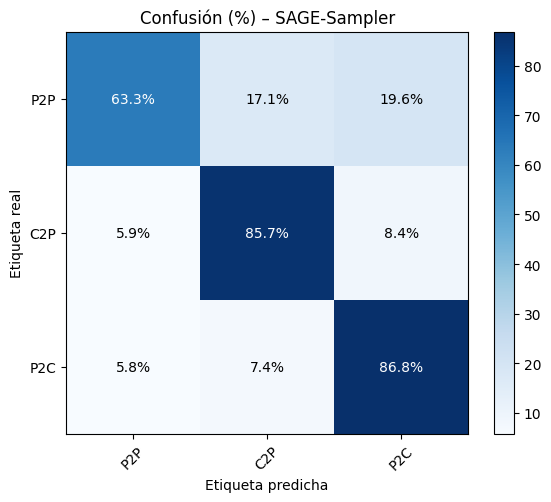
\includegraphics[width=\linewidth]{img//resultados//gnn//end-to-end//caso3/mc_graphsage_mlp_20neig.png}
        % \caption*{GraphSAGE + MLP}
        \label{fig:mc_graphsage_mlp_20nei}
    \end{minipage}
    \hfill
    \begin{minipage}[b]{0.32\linewidth}
        \centering
        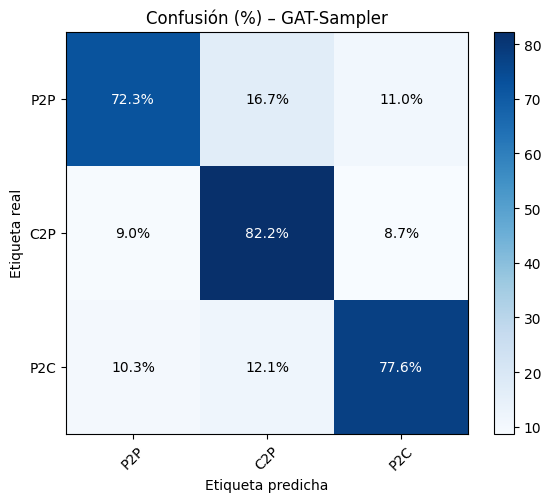
\includegraphics[width=\linewidth]{img//resultados//gnn//end-to-end//caso3/mc_gat_mlp_20nei.png}
        % \caption*{GAT + MLP}
        \label{fig:mc_gat_mlp_20nei}
    \end{minipage}

    \caption{Matrices de confusión para GCN, GraphSAGE y GAT usando decodificador MLP con 20 vecinos aleatorios por capa.}
    \label{fig:mc_gnns_mlp_20nei}
\end{figure}


Se logra ver que el uso de muestreo aleatorio de vecinos es una alternativa eficiente para entrenar modelos GNN en grafos grandes, permitiendo reducir la carga computacional sin sacrificar demasiado rendimiento. 
Específicamente para nuestro escenario, GCN alcanza el mejor resultado con una Accuracy de 92.18\%. El mejor resultado se obtiene con 20 vecinos, lo que nos dice que el muestreo de un mayor número de vecinos permite capturar más contexto estructural, reduciendo la pérdida de información.\\

%A medida que se incrementa la cantidad de vecinos muestreados por capa, se observa una mejora en el desempeño de los modelos, especialmente en la clasificación de las clases minoritarias (C2P y P2C). Con 10 y 15 vecinos, los modelos logran un mejor balance entre Precision y recall. Sin embargo, al llegar a 20 vecinos, el rendimiento disminuye en algunos casos, probablemente por información redundante o ruido. GAT se muestra más robusto ante este aumento, gracias a su mecanismo de atención, mientras que GraphSAGE es más sensible a este cambio.\\

%El modelo GAT aprovecha mejor el hecho de tener más vecinos gracias a su mecanismo de atención, que le permite asignar distintos pesos a cada nodo y priorizar la información más relevante. En cambio, GraphSAGE combina directamente la información de sus vecinos mediante agregación, lo que puede ser más perjudicial en escenarios con muestreo aleatorio, ya que no existe un criterio topológico para seleccionar vecinos y esto puede llevar a un muestreo poo representativo.\\


\subsubsection{Caso 3: Se utiliza grafo con atributos de PeeringDB y muestreo basado en comunidades (ClusterGCN)}

\begin{itemize}
    \item \textbf{RIBs:} Febrero 2024.
    \item \textbf{Atributos de nodos:} Dataset creado a partir de PeeringDB.
    \item \textbf{Esquema de entrenamiento:} Por \textit{batches}, aplicando \textit{ClusterGCN}.
    \item \textbf{Epochs:} 100.
    \item \textbf{Configuraciones evaluadas:} Tamaño de  clúster de 1000 nodos.    
    \item \textbf{Early Stopping:} Paciencia de 8 epochs.
    \item \textbf{Learning rate:} 0,01.
\end{itemize}


ClusterGCNSampler es un estrategia de muestreo que divide el grafo en clusters, y entrena usando mini-batches basados en esos subgrafos en lugar de todo el grafo.\\


\begin{table}[H]
\centering

\begin{tabular}{lcccc}
\toprule
\textbf{Modelo} & \textbf{Precision (\%)}  & \textbf{Recall (\%)} & \textbf{Accuracy (\%)} \\
\midrule
GCN & \textbf{89.16} & \textbf{89.21} & \textbf{89.16} \\
GraphSAGE & 89.16 & 89.22 & 89.11 \\
GAT & 79.92 & 78.40 & 78.54 \\
\bottomrule
\end{tabular}

\caption{Resultados de clasificación por modelo utilizando decodificador MLP con muestreo basado en comunidades (\textit{ClusterGCN}).}

\label{tab:caso3_mlp_clustergcn}
\end{table}




\begin{figure}[H]
    \centering
        \centering
        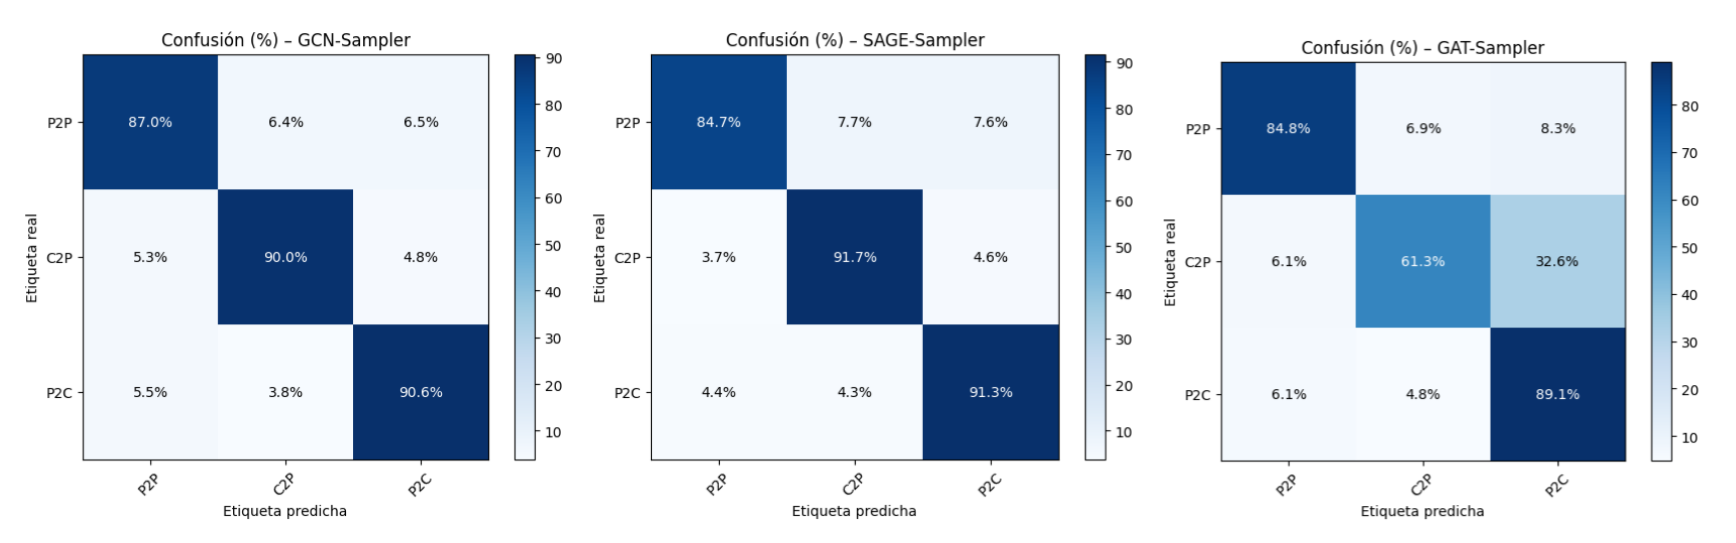
\includegraphics[width=\linewidth]{img//resultados//gnn//end-to-end//casoclustrgcn/clusterGCNMatrices.png}
        %\caption{GCN + MLP con ClusterGCN}
        \label{fig:mc_gcn_cluster}
    \caption{Matrices de confusión obtenidas utilizando diferentes modelos GNN (GCN, GraphSAGE y GAT) con decodificador MLP y clúster tamaño 10000.}
\end{figure}




Este caso demuestra que el muestreo por comunidades (ClusterGCN) es una opción viable para escalar en grafos grandes. Sin embargo, los resultados son inferiores a los obtenidos con full batch, lo que sugiere un trade-off entre escalabilidad y métricas de desempeño del modelo. Además, se observa que GAT pierde capacidad discriminatoria bajo este esquema.\\


%En comparación a los otros casos, el enfoque con ClusterGCN muestra un rendimiento intermedio. Aunque GCN y GraphSAGE alcanzan buenos resultados (87,83\% y 88,10\% de accuracy, respectivamente), estos son inferiores a los obtenidos en el Caso 0 (con atributos ricos de PeeringDB y entrenamiento full-batch), donde los mismos modelos superan el 92\% de accuracy. Esto sugiere que, si bien ClusterGCN permite escalar a grafos grandes con eficiencia, puede perder parte del contexto global al segmentar la topología del grafo en subgrafos desconectados.



%hay arly stopying n poch 40
 %En contraste, los resultados superan claramente a los del Caso 1, donde los nodos solo contaban con información de grado, y también son más estables que en el Caso 2 con muestreo aleatorio, especialmente para GAT, que presenta una degradación considerable con 20 vecinos. 
 
%     GCN clásico requiere toda la vecindad de cada nodo → no es batchable naturalmente.

%     ClusterGCN lo resuelve permitiendo entrenamiento por subgrafos precomputados.

% 3. Subgrafos más informativos

%     A diferencia del muestreo aleatorio (e.g., en GraphSAGE), los clusters suelen estar estructuralmente conectados, preservando mejor la topología del grafo.

    

%     Subgrafos más densos → mejores señales de entrenamiento.

%     Menos variabilidad por sampling → más estable que random neighbors.






% Algunas razones posibles son:

%     El modelo es simple o no tiene suficiente capacidad para sobreajustar incluso si quisiera (por ejemplo, pocas capas o parámetros).

%     El problema es fácil o las clases están bien separadas, por lo que el modelo no necesita memorizar ejemplos específicos.

%     Los conjuntos de entrenamiento y validación son muy similares (por ejemplo, por cómo hiciste el split, o si hay mucha redundancia entre ambos).

%     Regularización efectiva: Puede que uses dropout, weight decay o alguna técnica que evita el overfitting de forma natural.

%     Cantidad de datos: Si tienes muchos datos y el modelo es pequeño, es difícil que sobreentrene.






\subsubsection{Caso 4: Se utiliza grafo con atributos de nodos generados aleatoriamente}



\begin{itemize}
    \item \textbf{RIBs:} Febrero 2024.
    \item \textbf{Atributos de nodos:} Atributos generados aleatoriamente, tamaño 32.
    \item \textbf{Epochs:} 100. 
    \item \textbf{Early Stopping:} Paciencia de 10 epochs.
    \item \textbf{Learning Rate:} 0.01.
\end{itemize}


El objetivo fue evaluar cómo se comporta el modelo cuando los atributos de los nodos no contienen información estructural ni semántica. Para esto se generaron atributos aleatorios para los nodos del grafo con el fin de evaluar si la información estructural del grafo por sí sola es suficiente para realizar la tarea de inferencia y así comparar con los casos anteriores y analizar que tan importantes son los atributos utilizados previamente.\\



\begin{table}[H]
\centering
\begin{tabular}{lcccc}
\toprule
\textbf{Modelo} & \textbf{Precision (\%)} & \textbf{Recall (\%)}  & \textbf{Accuracy (\%)} \\
\midrule
GCN & \textbf{85.75} & \textbf{74.68} & \textbf{85.85} \\
GraphSAGE & 56.19 & 33.34 & 68.56\\
GAT & 63.02 & 61.86 & 77.73 \\
\bottomrule
\end{tabular}

\caption{Resultados de clasificación por modelo utilizando decodificador MLP. En Precision, recall y F1-score se muestran los valores promedio macro (clases 0, 1 y 2).}
\label{tab:caso4_mlp_random_attr}
\end{table}

\begin{figure}[H]
    \centering
    \begin{minipage}{0.32\textwidth}
        \centering
        
\includegraphics[width=\linewidth]{img//resultados//gnn//end-to-end//casorandom/mc_gcn_mlp.png}
  %      \caption*{GCN + MLP}
        \label{fig:mc_gcn_random}
    \end{minipage}\hfill
    \begin{minipage}{0.32\textwidth}
        \centering
        
\includegraphics[width=\linewidth]{img//resultados//gnn//end-to-end//casorandom/mc_graphsage_mlp.png}
 %       \caption*{GraphSAGE + MLP}
        \label{fig:mc_graphsage_random}
    \end{minipage}\hfill
    \begin{minipage}{0.32\textwidth}
        \centering
        
\includegraphics[width=\linewidth]{img//resultados//gnn//end-to-end//casorandom/mc_gat_mlp.png}
%        \caption*{GAT + MLP}
        \label{fig:mc_gat_random}
    \end{minipage}
    \caption{Matrices de confusión obtenidas utilizando modelos GCN, GraphSAGE y GAT con decodificador MLP con atributos aleatorios.}
    \label{fig:mc_random_all}
\end{figure}

Los resultados muestran que GCN es el único que alcanza resultados aceptables con una Accuracy de 85,9\% , mientras que GraphSAGE y GAT colapsan hacia la predicción trivial de la clase mayoritaria (P2P), sin lograr discriminar las clases C2P y P2C. Esto se debe a cómo cada arquitectura procesa la información; GCN utiliza una matriz de adyacencia, que le permite capturar patrones estructurales del grafo incluso en ausencia de atributos significativos. En cambio, GraphSAGE y GAT dependen fuertemente de la agregación de atributos de los vecinos y como en estos experimentos los atributos son aleatorios resulta en que los modelos predigan siempre la misma clase superior (P2P). Con esto podemos decir que, si bien la estructura del grafo por sí sola contiene información suficiente para que GCN mantenga un desempeño razonable, los atributos tienen un rol importante en las arquitecturas GNN. Por lo tanto, el uso de atributos resulta esencial para explotar plenamente el potencial de estos modelos en la inferencia de relaciones económicas.\\



%Los resultados muestran que GCN es el único modelo que alcanza un rendimiento aceptable, con una accuracy de 85,9%, mientras que GraphSAGE y GAT colapsan hacia la predicción trivial de la clase mayoritaria (P2P), sin lograr discriminar las clases C2P y P2C. Esto se debe a la forma en que cada arquitectura procesa la información: GCN utiliza una matriz de adyacencia normalizada, lo que le permite capturar patrones estructurales del grafo incluso en ausencia de atributos significativos. En cambio, GraphSAGE y GAT dependen fuertemente de la agregación de atributos de los vecinos y, dado que en este experimento los atributos son aleatorios, los embeddings resultan poco diferenciados, llevando a los modelos a predecir siempre la clase dominante (P2P). Con ello podemos concluir que, si bien la estructura del grafo por sí sola contiene información suficiente para que GCN mantenga un desempeño razonable, los atributos de los nodos juegan un rol fundamental en arquitecturas más complejas. Por lo tanto, el uso de atributos informativos resulta esencial para explotar plenamente el potencial de los modelos GNN en la inferencia de relaciones económicas.








%/////////////////////////////////////////////////
\section{Resultados del \textit{Benchmark} de métodos tradicionales} \label{sec:benchmark_result_section}

Para la inferencia de las relaciones comerciales entre Sistemas Autónomos, primero se ejecutaron los distintos métodos sobre los datos correspondientes a las fechas en que se recolectaron las RIBs. Para esto se ocuparon las primeras $1.000.000$ de rutas de \texttt{sanitized\_ribs.txt}. Como el dataset de evaluación (CAIDA AS Relationships) se ocuparía para métodos de deep learning, se tuvo que dividir en conjuntos de entrenamiento y evaluación. Además, este mismo dataset de evaluación se utilizó para evaluar todos los métodos, con el fin de mantener la consistencia en la comparación de los resultados. \\

\begin{figure}[H]
    \centering

    \begin{subfigure}[h]{0.48\textwidth}
        \centering
        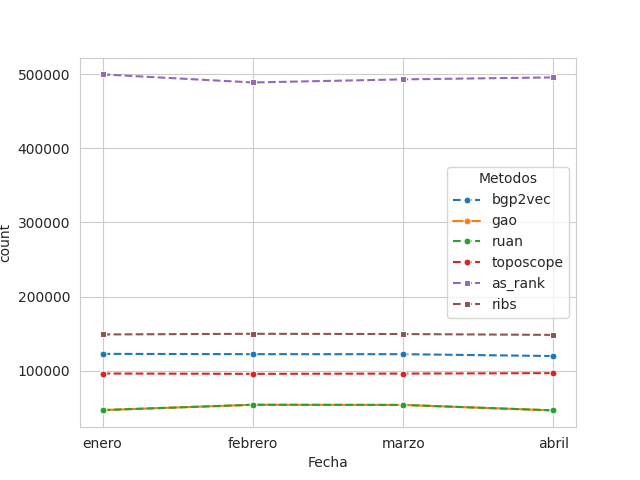
\includegraphics[width=\textwidth]{img/resultados/comparacion_metodos_cantidad.png}
        \caption{Cantidad de relaciones de los métodos para diferentes fechas.}
        \label{fig:comparacion_metodos_cantidad}
    \end{subfigure}
    \hfill
    \begin{subfigure}[h]{0.48\textwidth}
        \centering
        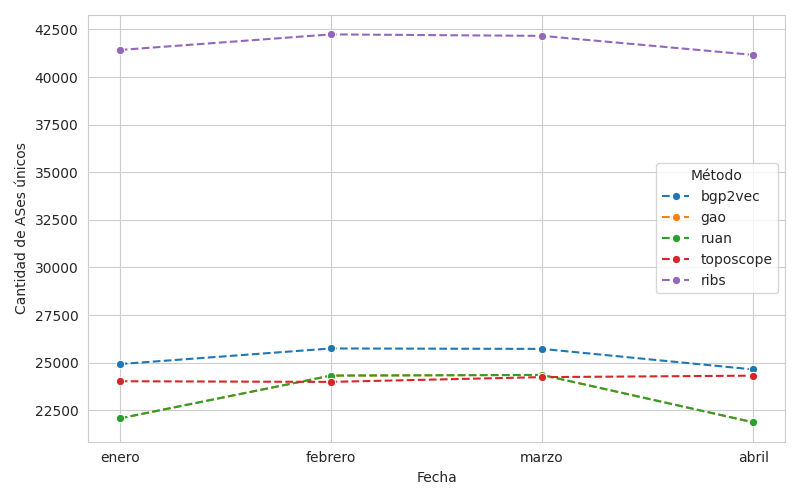
\includegraphics[width=\textwidth]{img/resultados/comparacion_metodos_cantidad_ASes.png}
        \caption{Cantidad de ASes de los métodos para diferentes fechas.}
        \label{fig:comparacion_metodos_cantidad_ASes}
    \end{subfigure}

    \caption{Cantidad de aristas inferidas y cantidad de ASes inferidos por cada método para distintas fechas.}


\end{figure}

Por esta razón, en la Figuras ~\ref{fig:comparacion_metodos_cantidad}  y \ref{fig:comparacion_metodos_cantidad_ASes} se muestran la cantidad de ASes y aristas inferidas por cada método, pues puede haber aristas que fueron inferidas pero no están presentes en el dataset de evaluación, así como aristas que sí están en el dataset pero no fueron inferidas por algunos métodos, lo cual es de esperarse dada la naturaleza del problema y las diferencias en los enfoques utilizados. Como era de esperarse, bgp2vec es el método que infiere la mayor cantidad de relaciones, ya que infiere todas las relaciones que se le proporcionan en el conjunto de test.\\


Se analizaron los enlaces inferidos y se vio si estos se mantenían constantes a lo largo de los distintos meses. Sin embargo, dado que solo se pudo utilizar una porción de las RIBs, los paths disponibles varían entre meses, lo que provocó que algunas relaciones estuvieran presentes en un mes pero ausentes en otros. Como resultado, el número de relaciones que coincidían en los cuatro meses fue muy reducido. Sin embargo, si se considera que una relación se mantiene constante si aparece en al menos dos meses, se obtiene la distribución presentada en la Figura~\ref{fig:relaciones_constantes_cambiantes_por_metodo}, donde en naranjo aparece la cantidad de enlaces que aparecen iguales en los cuatro meses en los que se ejecutaron los diferentes métodos y en rojo la cantidad que fue cambiando.\\

\begin{figure}[H]
    \centering
    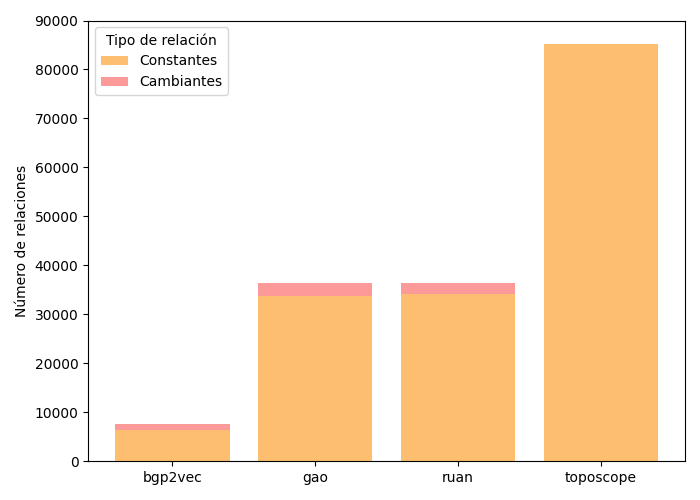
\includegraphics[width=0.7\textwidth]{img/resultados/relaciones_constantes_cambiantes_por_metodo.png}
    
    \caption{Constancia de relaciones con el tiempo}
    \label{fig:relaciones_constantes_cambiantes_por_metodo}
\end{figure}


\begin{table}[H]
\centering
\caption{Coincidencia entre métodos de inferencia en febrero}
\label{tab:comparacion_metodos_febrero}
\begin{tabular}{llrrr}
\toprule
Método 1 & Método 2 & Relaciones comparadas & Coincidencias & Porcentaje (\%) \\
\midrule
gao       & ruan       & 48.680 & 37.147 & 76.31 \\
gao       & toposcope  & 15.238 & 6.558  & 43.04 \\
gao       & bgp2vec    & 10     & 4      & 40.00 \\
ruan      & toposcope  & 15.238 & 3.922  & 25.74 \\
ruan      & bgp2vec    & 10     & 3      & 30.00 \\
toposcope & bgp2vec    & 13     & 6      & 46.15 \\
\bottomrule
\end{tabular}
\end{table}

La Tabla~\ref{tab:comparacion_metodos_febrero} muestra el grado de coincidencia entre distintos métodos de inferencia de relaciones AS durante el mes de febrero. Se observa una alta consistencia entre los métodos Gao y Ruan, con más del 76\% de coincidencias. En contraste con los métodos Toposcope y BGP2Vec que  presentan un menor grado de coincidencia, probablemente debido a diferencias metodológicas y a la cobertura de inferencia. La información presentada fue obtenida cruzando los \textit{datasets} de cada método para el mes de febrero, identificando las relaciones entre sistemas autónomos (AS) comunes entre pares de métodos.\\




Una vez ejecutados los diferentes métodos, se obtuvieron los valores de Accuracy que se presentan en la Tabla~\ref{tab:comparacion_accuracy}. 
%Los valores de Precision, Recall y F1-score correspondientes pueden encontrarse en las Tablas~\ref{tab:comparacion_presicion},  ~\ref{tab:comparacion_f1_score}, y ~\ref{tab:comparacion_recall} respectivamente, ubicadas en el Anexo~\ref{sec:bechmark_resultados}. \\


\begin{table}[H]
    \centering
    \begin{tabular}{lccccc}
    \hline
    \textbf{Método} & \textbf{Accuracy} \\
    \hline
    Gao & 81.77\% \\
    Ruan & 64.48\% \\
    ProbLink & 94.83\% \\
    TopoScope & 94.13\% \\
    bgp2vec & 94.51\% \\
    \hline
    \end{tabular}
    \caption{Comparación de resultados de \textit{Accuracy} entre distintos métodos.}
    \label{tab:comparacion_accuracy}
\end{table}

En la Figura~\ref{fig:relaciones_por_tipo_y_metodo} se muestra la cantidad de relaciones inferidas por tipo para cada uno de los métodos evaluados, donde claramente, bgp2vec es el método que infiere el mayor número de relaciones. Esto se debe a que su enfoque está basado en Machine Learning, el cual le permite inferir un tipo de relación para cada enlace presente en las rutas del conjunto de test. Además, se observa que bgp2vec tiende a inferir una gran cantidad de relaciones del tipo p2p. 
Por otro lado, Gao y Ruan infieren la misma cantidad total de relaciones, sin embargo, en esta figura se aprecia que, la distribución por tipo de relación es distinta.\\


\begin{figure}[H]
    \centering
    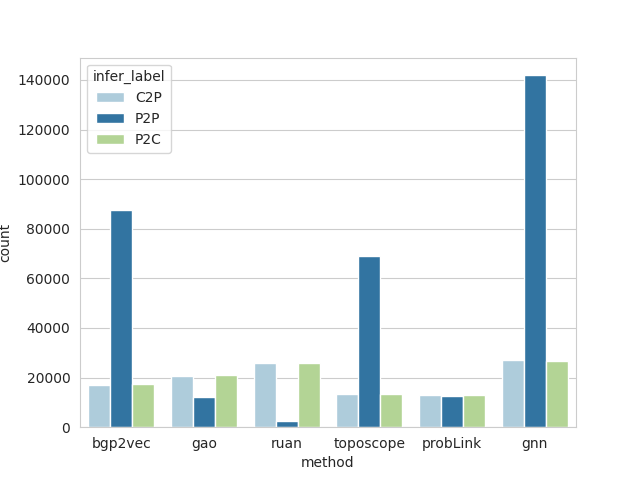
\includegraphics[width=0.7\textwidth]{img/resultados/benchmark/relaciones_por_tipo_y_metodo.png}
    \caption{Cantidad de relaciones por tipo para cada método para relaciones extraídas de RIBs de febrero de 2024.}
    \label{fig:relaciones_por_tipo_y_metodo}
\end{figure}


En las Figuras~\ref{fig:inferidos_correcta_icorrectamente_todo} y~\ref{fig:inferidos_correcta_icorrectamente_por_tipo} se presenta el conteo de relaciones inferidas correctamente e incorrectamente por cada método, y separadas por tipo, utilizando el conjunto de evaluación correspondiente a febrero de 2024.\\

\begin{figure}[H]
    \centering
    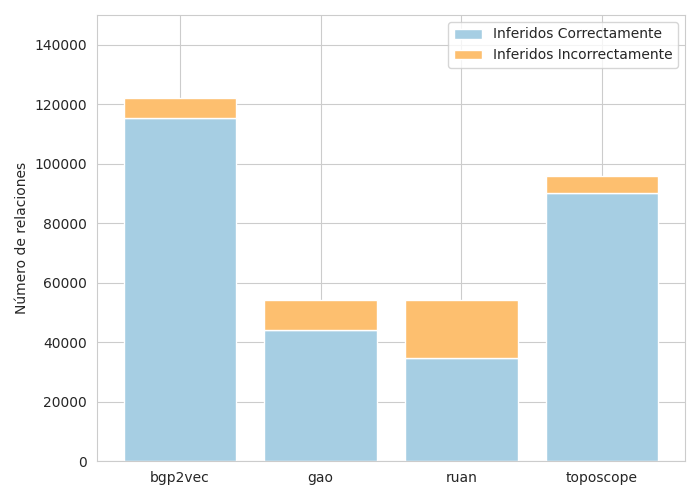
\includegraphics[width=0.7\textwidth]{img/resultados/inferidos_correcta_icorrectamente_todo.png}
    \caption{Cantidad de relaciones correctamente e incorrectamente inferidas por cada método para febrero de 2024.}
\label{fig:inferidos_correcta_icorrectamente_todo}
\end{figure}


\begin{figure}[H]
    \centering
    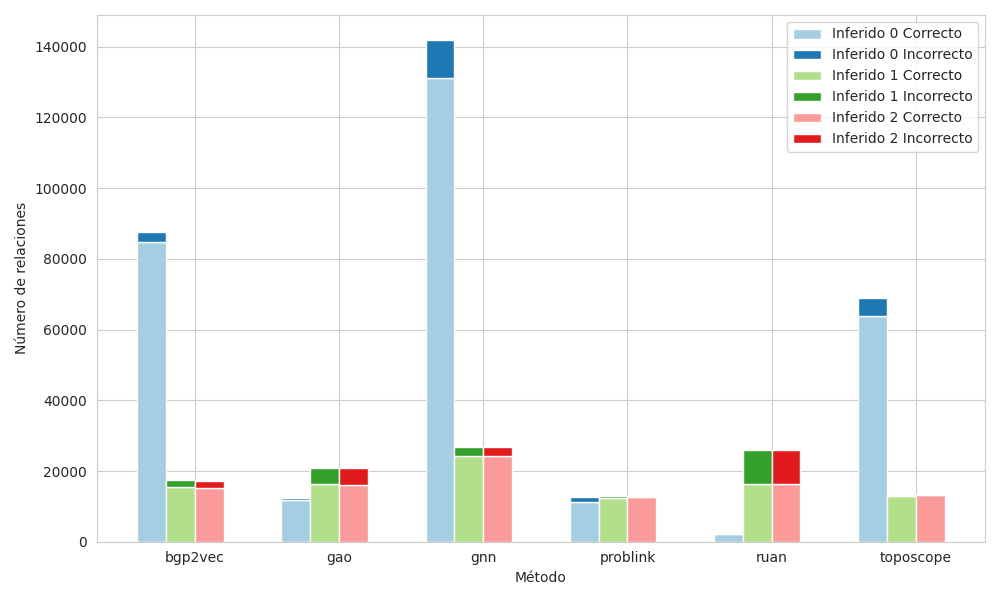
\includegraphics[width=0.8\textwidth]{img/resultados/benchmark/relaciones_inferidas_por_metodo_y_tipo.png}
    
    \caption{Cantidad de relaciones correctamente e incorrectamente inferidas, separadas por tipo, para febrero de 2024.}
    \label{fig:inferidos_correcta_icorrectamente_por_tipo}
\end{figure}

\newpage
Finalmente, al obtener las matrices de confusión para cada uno de los métodos, correspondientes al mes de febrero de 2024 (Figura~\ref{fig:comparacion-confusion}), se observa que las relaciones p2p son las más difíciles de inferir, ya que varios métodos tienden a confundirlas con c2p. Los métodos modernos como \textbf{ProbLink} y \textbf{TopoScope} ofrecen un mayor poder discriminativo, reduciendo significativamente la confusión entre pares P2P–C2P, mientras que los enfoques basados en \textit{embeddings} o heurísticas previas (BGP2Vec, Guo, Ruan) tienden a sobreclasificar las relaciones descendentes (c2p).




\begin{figure}[H]
    \centering

    \begin{subfigure}[t]{0.40\textwidth}
        \centering
        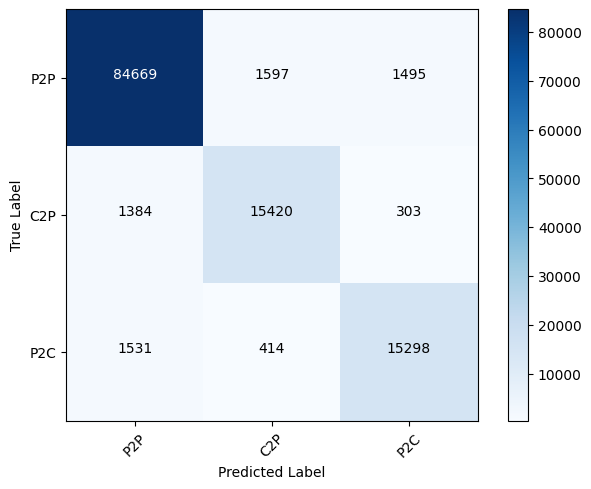
\includegraphics[width=\textwidth]{img/resultados/matrices_confusion/Confusion_matrix_bgp2vec_1m_febrero.png}
        \caption{BGP2Vec}
        \label{fig:confusion-bgp2vec}
    \end{subfigure}
    \hfill
    \begin{subfigure}[t]{0.4\textwidth}
        \centering
        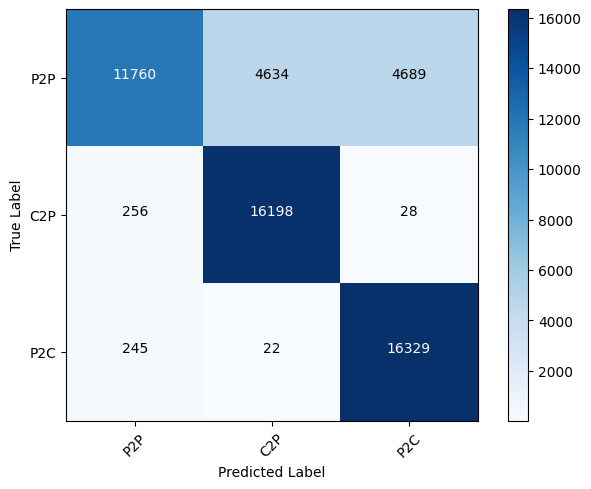
\includegraphics[width=\textwidth]{img/resultados/matrices_confusion/Confusion_matrix_gao_1m_febrero.png}
        \caption{Gao}
        \label{fig:confusion-gao}
    \end{subfigure}

    \vspace{0.75em}

    \begin{subfigure}[t]{0.4\textwidth}
        \centering
        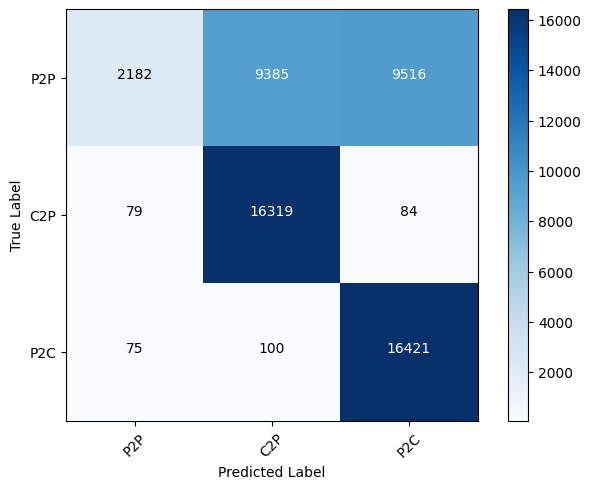
\includegraphics[width=\textwidth]{img/resultados/matrices_confusion/Confusion_matrix_ruan_1m_febrero.png}
        \caption{Ruan}
        \label{fig:confusion-ruan}
    \end{subfigure}
    \hfill
    \begin{subfigure}[t]{0.4\textwidth}
        \centering
        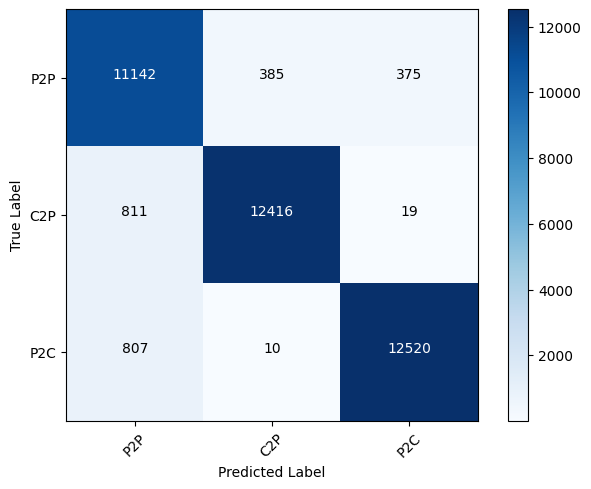
\includegraphics[width=\textwidth]{img/resultados/matrices_confusion/Confusion_matrix_problink_1m_febrero.png}
        \caption{ProbLink}
        \label{fig:confusion-problink}
    \end{subfigure}

    \vspace{0.75em}

    \begin{subfigure}[t]{0.4\textwidth}
        \centering
        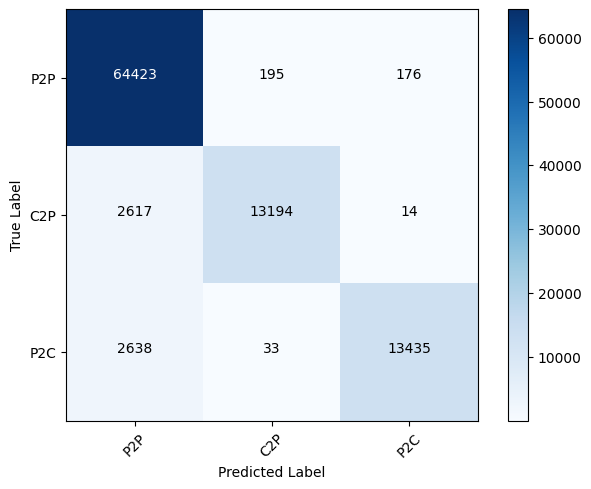
\includegraphics[width=\textwidth]{img/resultados/matrices_confusion/Confusion_matrix_toposcope_1m_febrero.png}
        \caption{TopoScope}
        \label{fig:confusion-toposcope}
    \end{subfigure}

    \caption{Matrices de confusión por método (febrero 2024).}
    \label{fig:comparacion-confusion}
\end{figure}


%El método GAO presenta una tendencia clara a confundir relaciones simétricas (P2P) con relaciones jerárquicas. En particular, se observan 4721 casos en que una relación P2P fue inferida como C2P, y 4636 casos en que fue clasificada como P2C. No obstante, el modelo demuestra alta Precision al inferir correctamente relaciones jerárquicas: 16.218 casos correctamente clasificados como C2P y 16.128 como P2C. Esto sugiere que GAO es un método confiable para la inferencia jerárquica, aunque tiende a subestimar la presencia de relaciones simétricas.\\


%Por su parte, el método RUAN presenta errores significativamente altos al momento de inferir relaciones P2P. Solo 2163 de estas relaciones fueron correctamente identificadas, mientras que más de 18.900 fueron clasificadas erróneamente como jerárquicas (9444 como C2P y 9502 como P2C). A pesar de esto, RUAN muestra un excelente rendimiento al clasificar relaciones jerárquicas, con 16.347 aciertos en C2P y 16.250 en P2C. Esta evidencia indica que RUAN comparte con GAO la fortaleza en jerarquías, pero presenta una marcada debilidad al reconocer relaciones simétricas.\\


%El método TOPOSCOPE presenta un comportamiento opuesto al de GAO y RUAN. Este clasificador tiende a sobreestimar las relaciones P2P, mostrando una gran cantidad de falsos positivos en esta categoría. Específicamente, 2645 relaciones reales C2P y 2620 P2C fueron clasificadas como P2P. Aunque logra un alto número de aciertos en esta clase (63.799), su tendencia a generalizar las relaciones como simétricas puede afectar negativamente la Precision en escenarios donde se requiere distinguir claramente las jerarquías.\\


%Finalmente, el método BGP2Vec demuestra el comportamiento más balanceado entre todos los métodos analizados. Sus errores se distribuyen de forma más equitativa entre las distintas clases, y mantiene un buen nivel de Precision en las tres. Clasifica correctamente 84.669 relaciones P2P, 15.420 C2P y 15.298 P2C. Aunque comete errores como P2P → C2P (1597), C2P → P2P (1384) y P2C → P2P (1531), la magnitud de estos es relativamente baja. Este resultado sugiere que BGP2Vec puede ser una alternativa más equilibrada para contextos en los que se requiere una cobertura general y menor sesgo por tipo de relación.\\


%El análisis de errores por tipo de relación muestra que cada método posee una estrategia inferencial distinta. Mientras GAO y RUAN priorizan la inferencia jerárquica y presentan dificultades con relaciones P2P, TOPOSCOPE privilegia las simétricas, a costa de errores en las jerárquicas. BGP2Vec, por otro lado, entrega una inferencia más homogénea y menos sesgada. Esta diversidad sugiere que una combinación inteligente de los métodos podría mejorar la robustez global del sistema de inferencia.\\

% \begin{itemize}
%     \item HAbalr de que bgp2vec tiene mayor cantidad de relaciones p2p y que s epuede deber a que el dataset de training tienen un numero superior de este tipo de enlaces, pro otro lado tmb s eve en los rsultados de las metricos. Es mas como hay muchos enlaces p2 si solo se infirieran todos los enlaces como op2p se tendria un resulatdo no mala de como XX.
%     \item Explciar por que ruan infiere tan pocas relaciones como p2p AAAAA
%     \item poner aquí todo de quien hace mejores o peores inferencias aquí poner todo lo que tengo que pensar y hacer sentido con los resultados de las métricas de arriba
% \end{itemize}






%Una particularidad que pudimos observar fue que al ejecutar los métodos con diferentes cantidad de rutas: primero con 1.000.000 de rutas y luego con 10.000.000. En el primer caso, el método de Gao obtuvo una accuracy de 80\%. Sin embargo, al ejecutarla 10.000.000 de rutas, la accuracy bajó a un 50\%, con estó se observó que, aumentó significativamente la cantidad de relaciones p2c y c2p, pasando de alrededor de 20.000 a aproximadamente 40.000 para ambas categorías, mientras que las relaciones p2p permanecieron casi constantes. Este mismo comportamiento se pudo observar también para el metodo de Ruan.\\






\section{Resumen}

En la tabla~\ref{tab:resumen_mejores_gnn_benchmark} se presenta un resumen comparativo de los resultados de los distintos experimentos, tanto para los enfoques basados en Redes Neuronales de Grafos como para los métodos preexistentes.\\
% Una vez obtenidos todos los resultados de los distintos experimentos, tanto para los dos enfoques basados en Redes Neuronales de Grafos como para los métodos preexistentes, se presenta en la Tabla~\ref{tab:resumen_mejores_gnn_benchmark} un resumen comparativo.  
% Este permite visualizar de manera más clara el desempeño de cada método en la tarea de inferencia de relaciones económicas entre Sistemas Autónomos.


\begin{table}[H]
\centering
\resizebox{\textwidth}{!}{
\begin{tabular}{llccc}
\toprule
\textbf{Método} & \textbf{Modelo / Configuración} & \textbf{Precision (\%)} & \textbf{Recall (\%)} & \textbf{Accuracy (\%)} \\
\midrule
\multicolumn{5}{l}{\textit{Benchmarks}} \\
\cmidrule(lr){1-5}
Heurístico   & Gao        & --   & --   & 81.77 \\
Heurístico   & Ruan       & --   & --   & 64.48 \\
Heurístico   & ProbLink   & --   & --   & \textbf{94.83} \\
Heurístico   & TopoScope  & --   & --   & 94.13 \\
\midrule
\multicolumn{5}{l}{\textit{Enfoque por etapas (Embeddings + Clasificador)}} \\
\cmidrule(lr){1-5}
Embeddings (PeeringDB, tarea: pred. aristas) & GraphSAGE + Dot Product & 86.08 & 83.87 & 85.04 \\
Embeddings (Grado nodos, tarea: pred. aristas) & GraphSAGE + Dot Product & 82.96 & 78.88 & 81.09 \\
Embeddings (Atributos estudio previo, tarea: pred. aristas) & GraphSAGE + Dot Product  & 85.14 & 82.18 & 83.76 \\
Embeddings (PeeringDB, tarea: pred. grado) & GraphSAGE + MLP & 84.61 & 79.65 & 82.29 \\
Embeddings (PeeringDB, tarea: pred. PageRank) & GraphSAGE + MLP & 86.74 & 83.58 & 85.17 \\
DeepWalk embeddings & -- & 87.54 & 85.43 & 86.43 \\
BGP2Vec embeddings & -- & \textbf{94.66} & \textbf{94.32} & \textbf{94.48} \\
\midrule
\multicolumn{5}{l}{\textit{Enfoque end-to-end (Encoder–Decoder)}} \\
\cmidrule(lr){1-5}
PeeringDB & GraphSAGE + MLP & \textbf{91.06} & \textbf{89.85} & \textbf{93.48} \\
Grado nodos & GCN + MLP     & 85.90 & 82.82 & 89.01 \\
PeeringDB + Random Neighbor Sampling & GCN & 90.85 & 86.25 & 92.18 \\
PeeringDB + ClusterGCN   & GCN + MLP & 89.16 & 89.21 & 89.16 \\
Atributos aleatorios  & GCN + MLP & 85.75 & 74.68 & 85.85 \\
\bottomrule
\end{tabular}
}
\caption{Resumen comparativo de los mejores resultados por caso y de los métodos de \textit{benchmark}.}
\label{tab:resumen_mejores_gnn_benchmark}
\end{table}



A continuación, se presenta un resumen de los aportes de cada experimento con aquello que fueron revelando respecto a la tarea de inferencia de relaciones económicas entre Sistemas Autónomos y la topología o relevancia de rasgos de Internet al momento de su uso en GNNs.
\vspace{0.5cm}
\begin{itemize}
    \item \textbf{Enfoque \textit{por etapas} (\textit{Embeddings} + Clasificador):}

    \begin{itemize}
        \item \textbf{Caso 0 (\textit{Embeddings} PeeringDB, tarea auxiliar: predicción de aristas):} Rendimiento sólido (Accuracy ≈ 85\%), confirma que los atributos de PeeringDB son informativos.

        \item \textbf{Caso 1 (\textit{Embeddings} con grado de entrada/salida):} Resultados más débiles (≈ 81\%), lo que evidencia que atributos muy básicos limitan el desempeño del modelo.

        \item \textbf{Caso 2 (\textit{Embeddings} con atributos de estudio previo – Giakatos):} ≈83–84\%, ligeramente inferior al obtenido con los atributos actualizados de PeeringDB 2024.
        Esto demuestra que los atributos diseñados en este trabajo son igual o más informativos que los utilizados en estudios anteriores, validando la pertinencia y calidad de las características extraídas.

        \item \textbf{Caso 3 y 4 (\textit{Embeddings} creados a partir de la predicción de grado/PageRank):}
        En estos casos, los \textit{embeddings} se preentrenaron con tareas auxiliares basadas en métricas estructurales.
        Los resultados muestran que PageRank aporta mayor información que el grado, ya que captura nociones de centralidad e influencia dentro de la topología global, permitiendo representaciones más ricas.
        Esta distribución sesgada provoca que las GNN converjan hacia valores promedio, limitando su capacidad para representar adecuadamente nodos muy centrales o periféricos.
        
        
        \item \textbf{Caso 5 (DeepWalk):} ≈ 86\%, muestra que los recorridos aleatorios logran capturar regularidades estructurales del grafo y reflejar de manera efectiva la proximidad entre nodos.
        Este resultado indica que, aun sin utilizar atributos adicionales, la topología por sí sola contiene suficiente información para inferir con buena Precision las relaciones entre Sistemas Autónomos.
        En comparación con los modelos que emplean atributos, DeepWalk alcanza un desempeño similar, lo que sugiere que los atributos disponibles aportan un valor complementario, pero no determinante, para esta tarea.
        %En otras palabras, el modelo demuestra que la estructura del grafo de Internet —y las conexiones que definen la posición relativa de los AS— es la fuente principal de información útil para la inferencia de relaciones.

        \item \textbf{Caso 6 (BGP2Vec):} ≈94.5\%, el mejor resultado del enfoque por etapas. A diferencia de DeepWalk, que modela la topología de manera puramente estructural, BGP2Vec incorpora la secuencia real de los caminos BGP, reflejando la frecuencia con que ciertos AS aparecen en las rutas. Esto hace que los nodos con mayor recurrencia en los caminos adquieran una mayor relevancia topológica, relacionada con su papel como proveedores de tránsito o puntos de interconexión clave.
        En consecuencia, los \textit{embeddings} de BGP2Vec representan no solo la conectividad, sino también la importancia funcional de los AS en la estructura jerárquica y económica de Internet, lo que explica su superior desempeño en la tarea de inferencia de relaciones.

        
    \end{itemize}
    
    \item \textbf{Enfoque \textit{end-to-end} (Encoder–Decoder):}
        \begin{itemize}
        \item \textbf{Caso 0 (PeeringDB, grafo completo):} El modelo GraphSAGE + MLP alcanza una Accuracy de ≈ 93.44\%, siendo el mejor resultado dentro de este enfoque y del estudio completo.
        Esto confirma que entrenar la GNN y el decodificador de forma conjunta permite optimizar directamente las representaciones para la tarea de inferencia, superando el rendimiento del enfoque por etapas y de los métodos del \textit{benchmark}.
    \item \textbf{Caso 1 (Atributo: grado de los nodos):}  
    Con solo el grado como atributo, GCN obtiene ≈ 89\%. Esto evidencia que, si bien la estructura del grafo aporta información relevante —particularmente el grado de conectividad de los nodos—, la ausencia de atributos más ricos, como los provenientes de \textbf{PeeringDB}, limita el rendimiento del modelo.  
    Este resultado refuerza la idea de que los atributos derivados de \textbf{PeeringDB} aportan señales semánticas esenciales para la tarea de clasificación.
     
    
    
    \item \textbf{Caso 2 (Random Neighbor Sampling):}  
    Con un muestreo de ≥ 20 vecinos, el modelo GCN mantiene un rendimiento alto (≈ 92\%) a la vez que reduce el costo computacional.  
    Este resultado demuestra que es posible entrenar en mini–batches sin una pérdida significativa de Precision, lo cual valida la escalabilidad del modelo para grafos grandes como el de Internet.  
    
    \item \textbf{Caso 3 (ClusterGCN):}  
    Los modelos GCN y GraphSAGE alcanzan ≈ 88–89\%, ligeramente inferiores al caso anterior.  
    Aunque esta técnica mejora la eficiencia para grafos extensos, tiende a perder información de frontera entre clusters, lo que afecta la calidad de las representaciones.  
    
    \item \textbf{Caso 4 (Atributos aleatorios):}  
    Solo GCN mantiene un rendimiento aceptable (≈85–86\%), mientras que GraphSAGE y GAT colapsan, clasificando la mayoría de los enlaces como P2P.  
    Este comportamiento evidencia que, si bien la estructura del grafo contiene información suficiente para generar representaciones básicas, la inclusión de atributos significativos es esencial para estabilizar el aprendizaje y evitar el sesgo hacia la clase mayoritaria.  
    \end{itemize}
\end{itemize}



%\subsection{Visualización y análisis de los \textit{embeddings}}

%Los \textit{embeddings} generados por los dos enfoques fueron luego proyectados en un espacio bidimensional utilizando técnicas de reducción de dimensionalidad, con el fin de visualizar si es que se podían observar patrones o agrupamiento entre ASes.\\

%En la Figura~\ref{fig:pca_embeddings} se puede observar la distribución global mediante la técnica PCA, donde los puntos tienden a  ....

%dispersarse de forma uniforme sin una separación evidente por tipo de relación. 
%En cambio, las proyecciones obtenidas con la técnica t-SNE y UMAP (Figuras~\ref{fig:tsne_embeddings} y~\ref{fig:umap_embeddings}) muestran ...
%una mayor tendencia a formar agrupamientos locales, indicando que los \textit{embeddings} capturan características estructurales relevantes del grafo.

%Estos resultados sugieren que el modelo ...
%logra representar a los ASes de forma coherente con sus interacciones, permitiendo una interpretación más intuitiva del espacio de representación aprendido.


%\begin{figure}[H]
%    \centering
%    \includegraphics[width=0.75\textwidth]{img/resultados/Embeddings/pca_embeddings.png}
%    \caption{Proyección de los \textit{embeddings} mediante PCA.}
%    \label{fig:pca_embeddings}
%\end{figure}

%\begin{figure}[H]
%    \centering
%    \includegraphics[width=0.75\textwidth]{img/resultados/Embeddings/tsne_embeddings.png}
%    \caption{Proyección de los \textit{embeddings} mediante t-SNE.}
%    \label{fig:tsne_embeddings}
%\end{figure}

%\begin{figure}[H]
%    \centering
%    \includegraphics[width=0.75\textwidth]{img/resultados/Embeddings/umap_embeddings.png}
%    \caption{Proyección de los \textit{embeddings} mediante UMAP.}
%    \label{fig:umap_embeddings}
%\end{figure}



































































%\section{Visualizacion}

%Para vr q las cosas tuvisn sntido se viualizaron los emb.
%Para hacier stos e dbio bajar la dimnsionalidad d e los vectors a 2d usndo dos mtodos acptados/%rcobocidos 


%\begin{itemize}
%    \item \textbf{pca:}
%    \item \textbf{t-SNE:} reducción de dimensionalidad no lineal pensada para preservar vecindades locales (útil para ver “clusters”).
%\end{itemize}





% %/////////////////////////////////////////////////////////////////
% \section{Análisis complementario de atributos mediante correlación}
% \subsection{Matriz de Correlación entre Atributos}

% En el contexto del Machine Learning una técnica de exploración y análisis de los datos es la construcción de una matriz de correlación entre los atributos. Esta permite visualizar relaciones lineales entre las variables del conjunto de datos y detectar posibles redundancias o patrones.\\

% \paragraph{¿Qué es una matriz de correlación?} Es una matriz cuadrada donde cada celda contiene un valor que indica el grado de correlación entre dos variables:
% \begin{itemize}
%     \item $+1$: correlación perfectamente positiva.
%     \item $-1$: correlación perfectamente negativa.
%     \item $0$: sin correlación lineal.
% \end{itemize}


% \paragraph{¿Por qué es útil en Machine Learning?}
% \begin{itemize}
%     \item \textbf{Detección de multicolinealidad:} si dos variables están fuertemente correlacionadas (por ejemplo, $|\rho| > 0.9$), pueden inducir redundancia en modelos sensibles como la regresión lineal.
%     \item \textbf{Selección de atributos:} facilita la eliminación de variables redundantes o la reducción de la dimensionalidad.
%     \item \textbf{Interpretabilidad:} permite comprender cómo se relacionan los datos antes de entrenar modelos.
% \end{itemize}

% \begin{figure}[H]
%     \centering
%     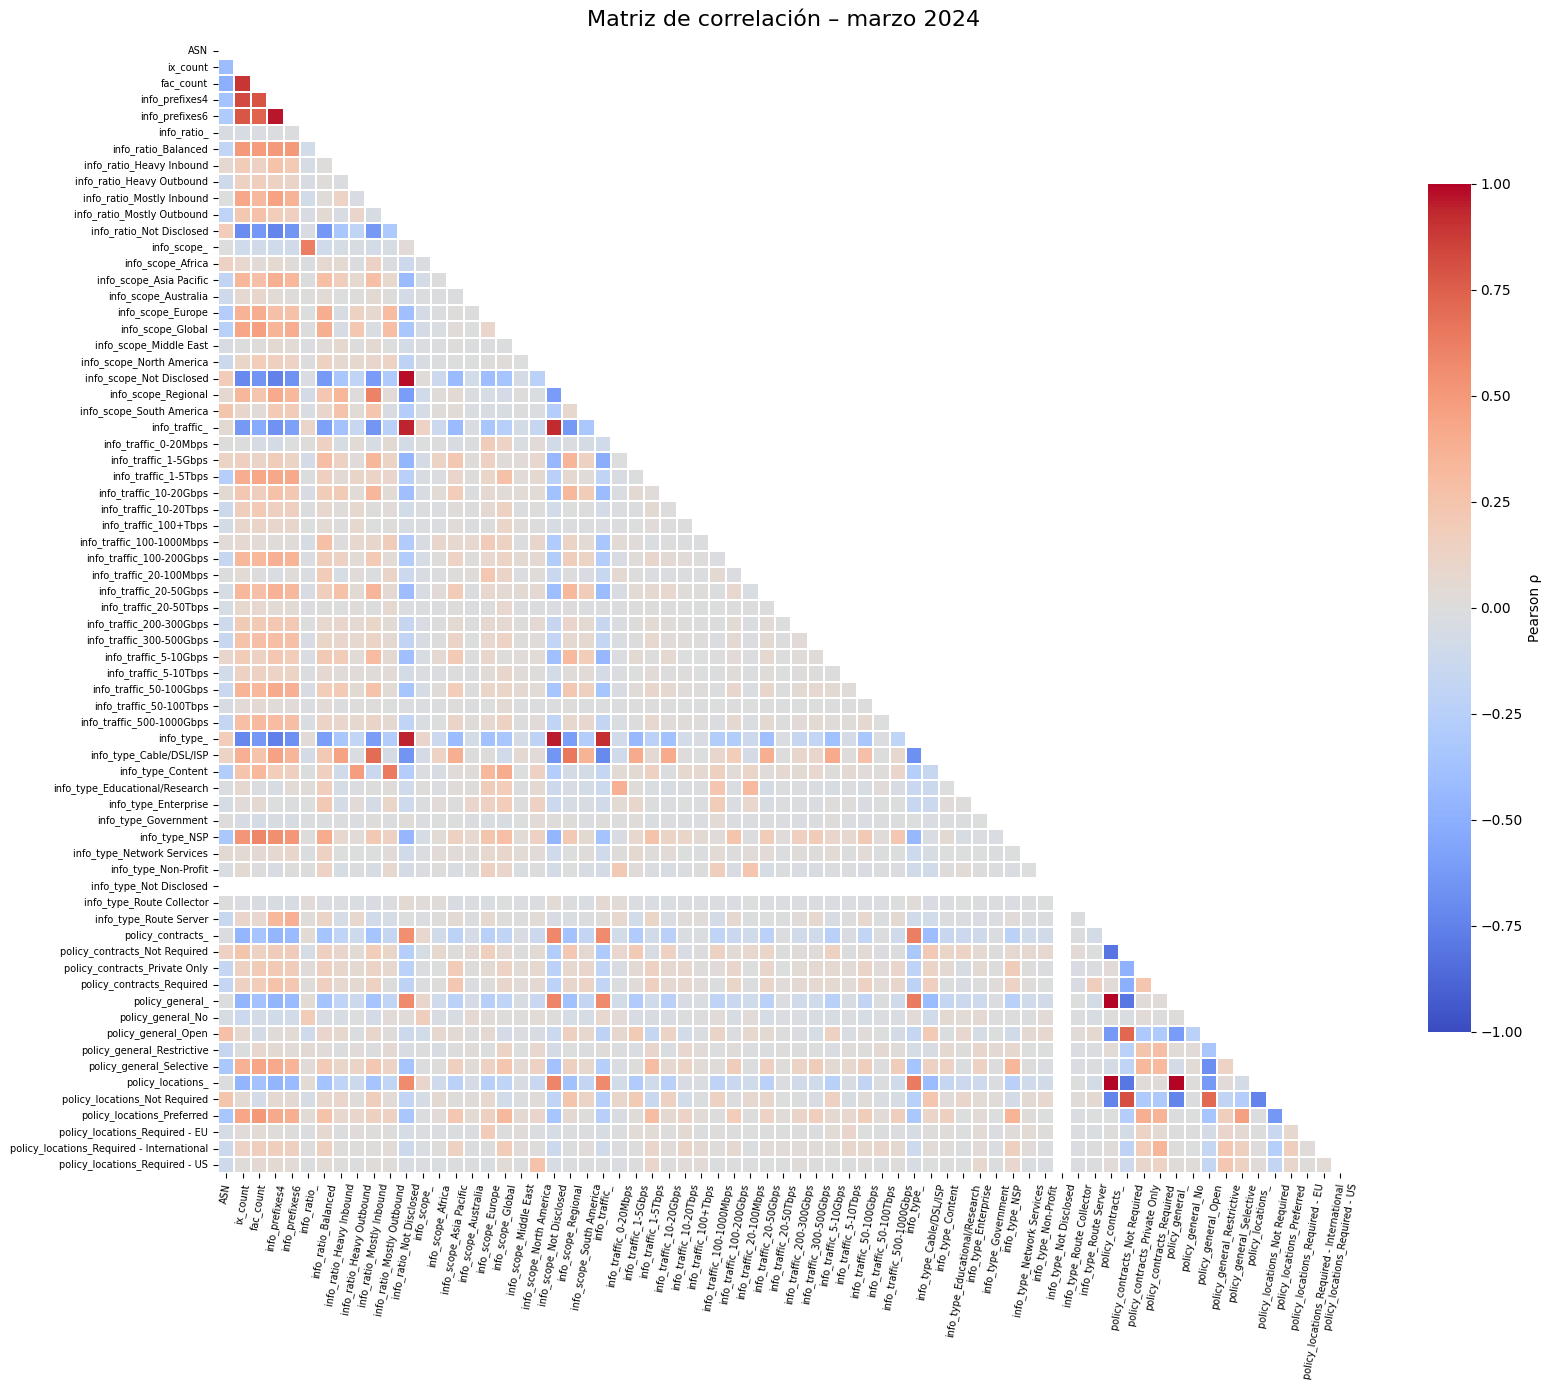
\includegraphics[width=\linewidth]{img/resultados/matriz_corr/matriz_corr_todos_attr.png}
%     \caption{Matriz de correlación de todos los atributos (febrero 2024).}
%     \label{fig:mat_corr_todos}
% \end{figure}

% Se calculó la matriz de correlación utilizando el coeficiente de Pearson. El valor en cada celda $\rho$ indica qué tan linealmente se relacionan dos variables, tomando valores entre $-1$ y $+1$. Para facilitar la visualización y el análisis, se extrajeron únicamente las correlaciones fuertes, es decir, aquellas donde $|\rho| \geq 0.5$.

% Se calculo la matriz de correlación usando el método de Pearson. Este valor en cada celda $\rho$ indica qué tan linealmente se relacionan dos variables. Una vez calculada y visualizada la matriz de correlación entre todos los atributos se quedo solo con las correlaciones fuertes tomando un umbral  $|\rho| \geq 0.5$, para una mejor visualización.


% \begin{figure}[H]
%     \centering
%     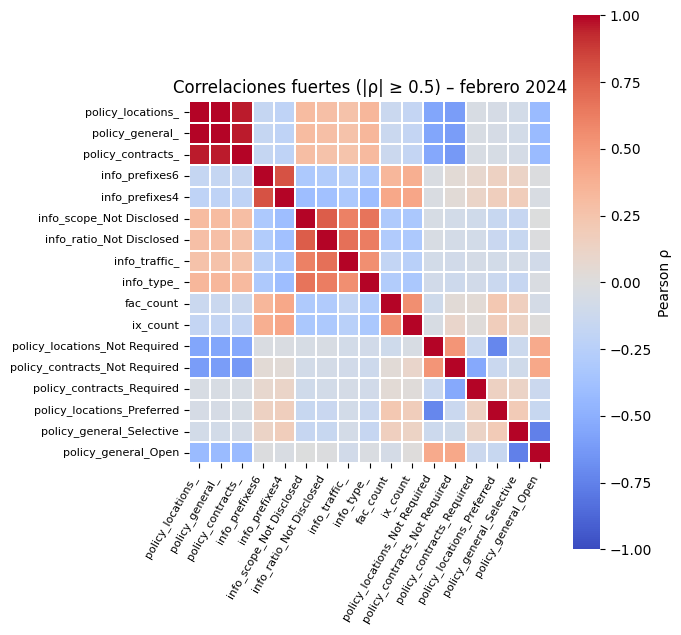
\includegraphics[width=0.65\linewidth]{img/resultados/matriz_corr/matriz_corr_febrero_altos.png}
%     \caption{Matriz de correlaciones fuertes ($|\rho| \geq 0.5$) entre atributos.}
%     \label{fig:mat_corr_fuerte}
% \end{figure}


% \paragraph{Interpretación de la matriz de atributos numéricos.}  
% En el mapa de calor, los colores indican la fuerza y dirección de la correlación:
% \begin{itemize}
%     \item Rojo intenso: correlación positiva fuerte.
%     \item Azul intenso: correlación negativa fuerte.
%     \item Celeste o gris claro: correlación débil o inexistente.
% \end{itemize}



% \begin{itemize}
%     \item \textbf{ix\_count/fac\_count:} los AS que aparecen en más IXPs suelen estar también presentes en más datacenters. Esto refleja que las redes grandes buscan mayor presencia física global.
%     \item \textbf{ix\_count/fac\_count – info\_prefixes4/6:} los AS con mayor conectividad física tienden a anunciar más bloques de direcciones IP (IPv4 e IPv6).
%     \item \textbf{info\_prefixes4 – info\_prefixes6:} presentan una correlación muy alta ($\rho > 0.80$), indicando que quienes anuncian muchos prefijos IPv4 también suelen anunciar muchos prefijos IPv6.
% \end{itemize}


% \begin{figure}[H]
%     \centering
%     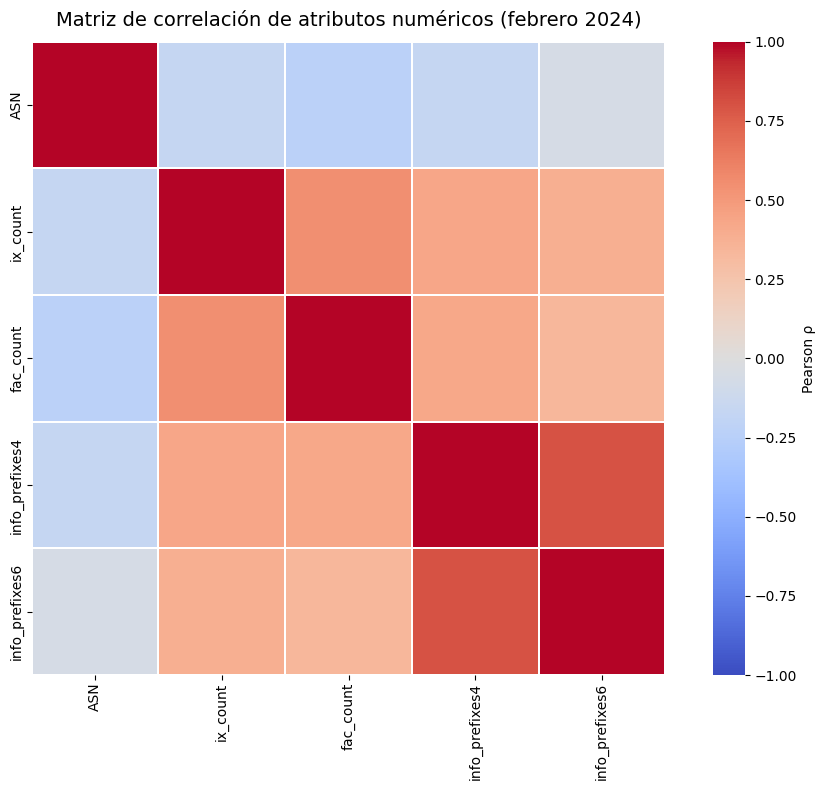
\includegraphics[width=0.6\linewidth]{img/resultados/matriz_corr/matriz_corr_attr_num.png}
%     \caption{Matriz de correlación entre atributos numéricos.}
%     \label{fig:mat_corr_numericos}
% \end{figure}




% %Esta informacion nos permite:
% %\begin{itemize}
% %    \item Optimizar el conjunto de atributos eliminando aquellos redundantes.
% %    \item Considerar la creación de indicadores agregados (por ejemplo, un índice de presencia global del AS).
% %    \item Asegurar que el modelo no se vea afectado por multicolinealidad, mejorando así su estabilidad y capacidad de generalización.
% %\end{itemize}


% %/////////////////////////////////////////////////////////////////
% \section{Análisis Embeddings Creados}

% \subsection{t-SNE}

% t-SNE es una técnica que “comprime” los vectores de alta dimensión (como tus embeddings) a sólo 2 dimensiones (o 3), tratando de preservar las distancias locales.\\

% Así, puedes visualizar en un gráfico plano cómo se agrupan, separan o mezclan los embeddings.

% Para visualizar si los embeddings que aprendió tu GNN tienen patrones interesantes:

%     ¿Los ASes similares están cerca?

%     ¿Se forman clusters claros?

%     ¿Las clases se separan en el espacio?

% Si ves grupos definidos o separaciones, normalmente es buena señal de que el embedding está “capturando” algo relevante




\chapter{Análisis y Conclusiones}

Este trabajo aborda el problema de la inferencia de relaciones comerciales entre Sistemas Autónomos (AS). Tarea fundamental para comprender el funcionamiento de Internet, optimizar su desempeño y detectar posibles anomalías. Se construyó un \textit{benchmark} que integra métodos previos (heurísticos y basados en Machine Learning), con el objetivo de establecer una línea base de comparación. Luego, se exploró la resolución de la tarea utilizando Redes Neuronales de Grafos (GNNs), evaluando su desempeño frente al \textit{benchmark}.\\


% RESULTADO BENCHMARK ------------------------------------

En el \textit{benchmark}, los métodos con mejor Accuracy corresponden a los métodos \textbf{ProbLink} (94,83 \%) y \textbf{BGP2Vec} (94,51 \%). Esto nos da a entender que enfoques probabilísticos y de Machine Learning (incluso en dos etapas, como BGP2Vec) capturan de mejor forma las características de los caminos de BGP.
Los métodos de BGP2Vec y Problink toman en cuenta tanto la información local (sus vecinos inmediatos) como la estructura global de la topología para etiquetar las relaciones; en cambio,  en contraste con los métodos de Gao\cite{InferringASRelatioships2001} y  Ruan\cite{Inferring-Multilateral-Peering}, realizan la inferencia basándose únicamente en la estructura observada en cada camino individual. 
Esto nos podría decir que, para inferir correctamente los tipos de relaciones entre Sistemas Autónomos, es fundamental tener el contexto global del enlace dentro de la topología de Internet, no es suficiente con conocer solo su posición dentro de un camino BGP (\texttt{AS\_PATH}) para una mejor inferencia.\\


% GNN (por etapas) -------------------------------------

Al pasar a las Redes Neuronales de Grafos (GNNs), específicamente \textit{por etapas} (donde primero se preentrenan los \textit{embeddings} y luego se utiliza un clasificador) se obtienen buenos resultados, con una Accuracy de alrededor de 85\%, superando a los métodos tradicionales de inferencia. Aquí también podemos notar que el uso de atributos de \textbf{PeeringDB}~\cite{PeeringDB}, en contraste con utilizar únicamente el grado, mejora la Accuracy (de 81.09\% a 85\%), dando a entender que las características asociadas de los ASes aportan información relevante para la inferencia. \\

Sin embargo, al utilizar los \textit{embeddings} generados por \textbf{DeepWalk} y \textbf{BGP2Vec}, que se construyen exclusivamente a partir de la estructura topológica del grafo, se alcanzan los mejores resultados dentro de este enfoque. Esto indica que la posición estructural de los AS dentro de la topología global de Internet es una fuente de información determinante para inferir correctamente las relaciones entre Sistemas Autónomos.\\

Finalmente, el mejor resultado dentro del enfoque por etapas con GNN se obtuvo al preentrenar los embeddings con la tarea auxiliar de predecir el valor de PageRank, lo que sugiere que incorporar nociones de centralidad y relevancia dentro de la topología ayuda a aprender representaciones más informativas para la clasificación, alineándose con lo dicho previamente.\\


% GNN (end-to-end) ------------------------------------
Al evaluar el enfoque \textit{end-to-end}, se obtuvieron los mejores resultados, alcanzando una Accuracy de 93.44\%, comparable con los métodos de mayor Accuracy del \textit{benchmark}.
De manera consistente con el enfoque por etapas, la inclusión de los atributos de PeeringDB~\cite{PeeringDB} resultó beneficiosa, mejorando la Accuracy de 89.01\% a 93.44\%, lo que demuestra que las características asociadas a este dataset enriquecen las representaciones aprendidas por la GNN. 
Por otra parte, en los experimentos diseñados se observó que, al usar atributos aleatorios, el modelo \textit{GCN} mantuvo un rendimiento aceptable (≈ 85\%), mientras que \textit{GraphSAGE} y \textit{GAT} colapsaron, clasificando la mayoría de los enlaces como P2P.\\







Estos resultados respaldan dos conclusiones:
\begin{itemize}
    \item La estructura del grafo por sí sola contiene información suficiente para aproximar la topología y las relaciones entre AS.
    \item La inclusión de atributos como PeeringDB nos permite alcanzar un mejor rendimiento en la inferencia de relaciones comerciales entre Sistemas Autónomos.
\end{itemize}

Además, los resultados obtenidos permiten observar ciertas propiedades estructurales de la topología de Internet y su impacto en el uso de GNNs. Internet muestra una distribución \textit{long-tail} en muchos de sus atributos (grado, centralidad, tráfico), donde pocos nodos (ASes grandes o Tier-1 que conforman el \textit{core}) concentran la mayoría de las conexiones, mientras que la gran mayoría posee una conectividad baja (periferia). Esto provoca que, al entrenar GNNs, los atributos (como el grado) no siempre generen \textit{embeddings} representativos o, en el enfoque \textit{por partes}, se tienda a generalizar. 
Esto explica por qué arquitecturas como GraphSAGE y GAT, que enfatizan la agregación de información desde vecinos seleccionados o ponderados, presentan un rendimiento más inestable, mientras que GCN, al basarse en una agregación más homogénea y en la normalización de la matriz de adyacencia, logra capturar mejor la estructura global incluso en estos escenarios (Caso 3 y 4 del enfoque \textit{por etapas}). \\

Por otro lado, los experimentos también evidencian la ``trampa de la Accuracy'' ya que dado que la clase P2P es la más frecuente en el dataset, un modelo que clasifica todos los enlaces como P2P puede alcanzar una Accuracy alta sin realizar una inferencia real, como en el caso~4 del enfoque \textit{end-to-end}. 
Por ello, métricas como el recall resultan de gran importancia para evaluar esta tarea.\\


Para cerrar, y en vista del trabajo realizado, se propone el siguiente trabajo futuro:
\begin{itemize}
    \item Incorporar atributos dinámicos o temporales, por ejemplo, información proveniente de mensajes \textit{BGP updates}, que permita capturar la evolución temporal de las relaciones entre Sistemas Autónomos.

    \item Ampliar el dataset mediante la integración de nuevas fuentes de datos, como mediciones de \textit{traceroute}, para complementar la visión obtenida desde BGP y construir una representación más completa de la topología de Internet.
    
    \item Evaluar los resultados del modelo en escenarios de detección de anomalías como \textit{route leaks}, \textit{hijacks} u otros eventos anómalos, comparando su rendimiento con métodos existentes.
    
    \item Analizar los \textit{embeddings} generados por las GNN, con el objetivo de estudiar qué propiedades topológicas o atributos capturan y cómo estas representaciones se relacionan con el rol y la posición de los AS dentro del grafo.
    
\end{itemize}
    
























% Primero debemos tener en cuenta que la metrica de Accuracy puede ser engañosa con clases desbalanceadas y en nuestro caso scomo se vio en la Figura X tenmos clases sueprp desbalanceadas, dond ela mayotit a de relaciones son P2Py al rededor d ela mitad p2Cy C2P.
%     Si el 90\% de tus datos son clase "P2P", un modelo que siempre predice "P2P" tendrá 90% de Accuracy… ¡aunque falle completamente las otras clases!


%Para visualizar mejor que esta pasando ocupamos las matrices de confusión, donde podemos ver .... 
% Tus clases son P2P, C2P, P2C. Si una clase es más frecuente, la Accuracy puede esconder errores. Por eso:

%     Usa matriz de confusión para ver qué clases se confunden.

%     Calcula precision, recall y F1-score por clase.

%     La Accuracy puede ser tu métrica global final, pero acompañada de las demás.





% Con estos resultados podemos decir que crear embeddings a partir de link prediction no es una buena metrica para crear la segund atask no rsulva bin y s qud aatascada=o n cirto punto a difrncia d bgp2vc q llga a una mjor acucracy y ovrall rsultados. como sabemos cual sra la mejromtricas para crera mbddinsg?






% CONCLUSION FINAL ---------------------------------------


%El estudio confirma que es factible construir un marco comparativo y competitivo para inferir relaciones AS: los métodos probabilísticos y de DL en dos etapas marcan un listón alto, pero un GNN end-to-end bien diseñado y con atributos adecuados puede situarse muy cerca del estado del arte. La estructura del grafo aporta información sustantiva —en particular con arquitecturas tipo GCN—, aunque la inclusión de atributos de calidad es determinante para superar ambigüedades locales. De cara al futuro, reforzar la capa de datos (más cobertura y temporalidad), enriquecer atributos y adoptar arquitecturas GNN sensibles al tiempo y a la escala de Internet debería traducirse en modelos más estables, precisos y útiles para operadores y analistas de infraestructura.



% RESUMEN -----------------------------------------------
%En síntesis, las contribuciones principales son: (1) la construcción de un benchmark reproducible que integra y estandariza métodos heterogéneos (heurísticos, probabilísticos y de aprendizaje profundo), con evaluación común sobre el mismo subconjunto de CAIDA; (2) la demostración de que un modelo GNN end-to-end, bien alimentado con atributos de PeeringDB, puede aproximar el rendimiento de métodos fuertes como ProbLink y BGP2Vec, manteniendo además interpretabilidad a nivel de señales de grafo; y (3) una caracterización de la sensibilidad a los atributos y a la disponibilidad de paths, útil para futuras campañas de medición.

%\section{Limitaciones y líneas futuras}
%Entre las limitaciones destacan: (i) el uso de RIBs de días específicos/ventanas acotadas, que priorizan el “core” de Internet y pueden sub-representar periferia, afectando la estabilidad temporal; (ii) el desbalance por tipo de relación (p. ej., predominio de c2p/p2c frente a p2p en ciertas vistas), que incide en confusiones observadas en algunos modelos; y (iii) la dependencia de atributos externos (PeeringDB), cuya calidad/actualización impacta directamente el desempeño. Ampliar la recolección (múltiples vantage points y días por mes), incorporar información temporal explícita (series de RIBs) y explorar GNNs temporales o ricas en atención multi-cabeza pueden mejorar robustez y generalización. Integrar señales adicionales (políticas, comunidades BGP, IXP/Route Servers) y técnicas de aprendizaje semi-supervisado/auto-supervisado también parece promisorio para reducir la necesidad de etiquetas y aprovechar la enorme estructura latente del grafo Internet.







%¿Qué pasa con la Accuracy en escenarios desbalanceados?
%La Accuracy mide el total de predicciones correctas sobre todas las clases.

%Si el dataset está desbalanceado (ej: hay muchísimas más relaciones p2p que c2p o p2c), un modelo puede “hacer trampa”: basta con que clasifique casi todo como p2p, y ya tendrá una Accuracy aparentemente alta.

%Pero en realidad estaría ignorando por completo las otras clases, lo que genera un modelo inútil para el problema real.


%Ejemplo ilustrativo:

%Dataset: 80\% p2p, 10\% c2p, 10\% p2c.

%Modelo: predice siempre p2p.

%Accuracy = 80\%.

%Pero recall para c2p y p2c = 0 (nunca las acierta).



%¿Qué hacer para un análisis correcto?

%Tienes que mirar métricas que no dependan tanto del desbalance:

%Recall por clase: te dice si el modelo está detectando las clases minoritarias.

%Precisión por clase: cuántos de los predichos son correctos.

%Matriz de confusión: muestra claramente en qué clases el modelo se equivoca.



%- por q graphs sage tiende a tner mejors resulatdos q las otras? para casos espcificos?
%- por q DP tiend tnmb a tner mejors rsultados q las MLP?


%\input{Capitulos/7-Experimentos}
% \chapter{Resultados}][_]
% \chapter{Conclusiones}

% REFERENCIA
\bibliography{library}

% ANEXOS

\begin{appendixs}
	% \section{Fundamentos de Internet y BGP} \label{sec:anexo_fundamentos_internet_bgp}

\subsection{Internet} \label{sec:anexo_internet}
Entidades y Jerarquías de Internet
La IANA (Internet Assigned Numbers Authority) es el stock central de bloques IP y ASN. Gestiona globalmente los bloques de direcciones IP y los ASN.

RIRs (Regional Internet Registries)
Las Autoridades Regionales de Registro de Internet (RIR) son organizaciones que gestionan la distribución de recursos de Internet (Ej: direcciones IP y ASN).

ARIN (América del Norte, parte del Caribe y algunas islas del Pacífico)
RIPE NCC (Europa, Oriente Medio y Asia Central)
APNIC (Asia y la región del Pacífico)
LACNIC (América Latina y el Caribe)
AFRINIC (África)

IETF (Internet Engineering Task Force)
Define los estándares técnicos (protocolos como BGP, TCP/IP, DNS, etc.).
No gobierna, sino que coordina cómo debe funcionar Internet.
ICANN (Internet Corporation for Assigned Names and Numbers)
Administra los nombres de dominio (.com, .org, .cl) y las direcciones IP.
A través de organizaciones regionales, delega bloques de IP y autonomía.
ISPs (Internet Service Providers)
Proveen conectividad a usuarios, empresas o a otros ISPs.
Van desde grandes proveedores globales hasta pequeños locales.


























\subsection{Sistemas Autónomos} \label{sec:anexo_sistemas_autonomos}


Como se habló previamente en la Sección~\ref{sec:sistemas_autonomos}, los \textbf{Sistemas Autónomos (AS)} son un conjunto de dispositivos que comparten un mismo protocolo de ruteo y están administrados por una misma entidad, cuya interconexión forma \textbf{Internet}.\\

Los \textbf{AS} se identifican mediante un número de \textbf{Sistema Autónomo (ASN)} de 16 bits y controlan un conjunto de direcciones \textbf{IP}. 
Esta asignación es llevada a cabo por los \textbf{Registros Regionales de Internet} (\textit{Regional Internet Registries}, \textbf{RIRs}), quienes reciben bloques de direcciones IP desde la \textbf{Autoridad Asignadora de Números de Internet} (\textit{Internet Assigned Numbers Authority}, \textbf{IANA}) y los distribuyen a los \textbf{Registros Locales de Internet} (\textit{Local Internet Registries}, \textbf{LIRs}) y a los usuarios finales.\\

Los \textbf{Proveedores de Servicios de Internet} (\textit{Internet Service Providers}, \textbf{ISP}), que pueden estar conformados por uno o varios Sistemas Autónomos, se dividen comúnmente en tres niveles de jerarquía:  
el \textbf{Tier-1}, donde se encuentran los AS que conforman el \textit{backbone} de Internet y que intercambian paquetes entre sí sin costo asociado;  
los \textbf{Tier-2}, generalmente operadores nacionales que compran tránsito a los Tier-1 y venden tránsito a los Tier-3;  
y finalmente los \textbf{Tier-3}, operadores locales que pagan por el tránsito para proporcionar acceso a Internet a los usuarios finales~\cite{InterconnectionPeeringSettlements}.  
Además, Luckie \textit{et al.}~\cite{ASRank} analizó los AS y propuso una métrica para indicar qué tan global es un AS:  
si el \textit{customer cone} es mayor o igual a 200, se considera Tier-1;  
si es mayor a 2,000, se considera Tier-2;  
y si es menor a 200, se considera Tier-3.\\

Una última clasificación que puede hacerse entre AS depende de sus conexiones a otros Sistemas Autónomos, dividiéndolos en \textbf{\textit{single-homed}} y \textbf{\textit{multi-homed}}.  
Los AS \textit{single-homed} tienen solo una conexión a otro AS, mientras que los \textit{multi-homed} poseen conexiones a más de un AS.\\



En la estructura de Internet, un Sistema Autónomo (AS) consiste en un conjunto de routers y enlaces de comunicación que comparten una política de enrutamiento común. Estos son operados independientemente por una organización (Ej: ISPs , universidades, empresas, entre otras). Definen/Utilizan uno o más bloques de direcciones IP que le han sido asignados por un RIR (Regional Internet Registry) o NIR. 

Existen 3 tipos de Sistemas Autónomos:
Stub: se conecta únicamente con un sistema autónomo.
Tránsito o proxy: se conecta con varios sistemas autónomos y además permite que se comuniquen entre ellos.
Multihomed: se conecta con varios sistemas autónomos, pero no soporta el tráfico de tránsito entre ellos.


Multi-origin AS : (MOAS) Algunos prefijos se originan desde múltiples Sistemas Autónomos (pueden ser siblings o ASes de diferentes organizaciones)
En BGP , el ORIGIN se ve al final del AS PATH.
Por que ocurre?
Anycast: El mismo prefijo anuncia desde varios AS/POPs para acercar el servicio al usuario.
Migración/transición de proveedor: Una red cambia de ASN o de Upstream y durante el cambio se ve el prefijo en dos orígenes.
Multihoming o mala configuración: Un cliente y su proveedor (o dos proveedores) terminan anunciando el mismo prefijo como origin por error.
MOAS conflict/secuestro o route leaks: Alguien anuncia un prefijo que no le corresponde, y BGP lo acepta si no hay filtros/ROV.


¿Qué es un Upstream?
Tu proveedor hacia Internet . Es hacia arriba en la cadena.
¿Qué es un Downstream?
Tus clientes o redes que dependen de ti para salir de Internet. Es hacia abajo en la cadena.

ASN privados y públicos.

Números de Sistemas Autónomos (ASN)

Es un identificador único para los Sistemas Autónomos, consisten en 16 o 32 bits  que definen identificadores números entre 0 a 65535 (definidos en la RFC 1930) y entre 0 y  4294967295 (definidos en la RFC 4893). Son asignados por un RIR o un NIR.

La Autoridad de Asignación de Números de Internet (IANA) ha reservado 1.023 de ellos (de 64.512 a 65.534) para uso privado. 

Existen dos tipos de ASN:

ASN Públicos:  Asignados por los  RIRs, son únicos a nivel mundial. Se utilizan para el enrutamiento en Internet y son visibles en las tablas de enrutamiento globales.
Son únicos en todo el mundo.
Se usan cuando tu red anuncia prefijos por BGP al resto de Internet.
Permiten que otros AS sepan quién eres y cómo llegar a ti.

ASN Privados: Son utilizados dentro de redes privadas y no son visibles en las tablas de enrutamiento globales. Los rangos de ASN privados son 64.512 a 65.534 y 4.200.000.000 a 4.294.967.294.
Sirven para:
Pruebas de BGP.
Conexiones internas entre routers.
Simulaciones o entornos cerrados.
	Si un router con ASN privado intenta anunciar un prefijo al Internet público, los 
demás routers lo filtran automáticamente (no lo propagan).


Ejemplos:
AS15169 → Google
AS3356 → Lumen (Level3)
AS65001 → Red privada (empresa o laboratorio)






\subsection{Internet Exchange Points} \label{sec:anexo_internet_exchange_points}
Los \textit{Internet Exchange Points} (IXPs) son puntos de interconexión donde múltiples ASes pueden establecer relaciones de peering con otros ASes \cite{Computer-Networking}.\\

Un IXP consiste generalmente en un switch  o router de alta velocidad y capacidad que conecta routers de diferentes ASes, permitiendo el intercambio directo de tráfico sin necesidad de atravesar redes intermedias. Mejorando así el intercambio de tráfico, haciéndolo más eficiente y de bajo costo.\\

% FIXME: arregalr redaccion
Las relaciones de tráfico en un IXP se establecen mediante el protocolo BGP, y el IXP solo actua como un intermediario. De esta forma por ejemplo un ISP en vez de estar conectados a multiples ASes  en una coneccion punto a punto, puede conectarse unicamente al IXP y como estos otros ASess tambien estaran conectados al IXP se ahorra recuersos fisicos y de administracion.\\

Al igual que los ASes, los IXPs tienen un ASN. Sin embargo, de forma generalizada, este ASN se extrae de los AS PATH en BGP. Algunos IXPs lo mantienen visible como método de debugging \cite{InferringASRelatioships2001}. 


\subsection{Ruteo} \label{sec:anexo_ruteo}
\subsubsection{Ruteo interno} \label{sec:anexo_ruteo_interno}
\subsubsection{Ruteo externo} \label{sec:anexo_ruteo_externo}





\subsection{BGP} \label{sec:anexo_bgp}

BGP es un Protocolo PATH Vector


Prefijos IP y su propagación en BGP


¿Qué es un prefijo IP?

Un prefijo IP o un bloque de IPs es una forma compacta de representar un conjunto continuo de direcciones IPs.
Se escrib con notación CIDR (Classless Inter-Domain Routing):

192.0.2.0/24 → representa 256 direcciones (desde 192.0.2.0 hasta 192.0.2.255)
2001:db8::/32 → prefijo IPv6 (bloque muy grande, miles de subredes posibles)

La parte /24 indica cuántos bits son la porción de red, y el resto son los bits disponibles para hosts.
Mientras más grande el número (por ejemplo /30 o /31), más pequeño el bloque.

¿Qué hace BGP con estos prefijos?

El Border Gateway Protocol (BGP) es el protocolo que permite a los Sistemas Autónomos (AS) intercambiar información de ruteo en Internet.
Cada AS anuncia los prefijos que posee o puede alcanzar, y esos anuncios se propagan a través de sus vecinos BGP.


AS
Prefijo que anuncia
Vecino
AS64500
203.0.113.0/24
AS64501
AS64501
203.0.113.0/24
AS64502
AS64502
203.0.113.0/24
Internet



Así, el bloque 203.0.113.0/24 “se propaga” por la red global BGP hasta que todos los routers del mundo saben que ese prefijo se alcanza a través de AS64500 (con su respectivo camino \texttt{AS\_PATH}).

Propagación de prefijos: el mecanismo

Cuando un router BGP recibe un anuncio de prefijo, no reenvía todo automáticamente. 
Sigue una serie de reglas y políticas:
Recibe un anuncio (por ejemplo: 200.7.4.0/22 via AS1234).
Guarda en su tabla BGP el prefijo junto con atributos:
\texttt{AS\_PATH}: secuencia de AS atravesados.
\texttt{NEXT\_HOP}: IP del siguiente router.
\texttt{LOCAL\_PREF}, MED, etc.
Evalúa políticas locales (ej. preferir clientes sobre peers).
Anuncia a otros vecinos según sus políticas (por ejemplo, a sus clientes, pero no siempre a otros peers).







Tabla de enrutamiento global vs. tabla local


tabla de enrutamiento global (BGP global routing table) y la tabla de enrutamiento local.
Cuando hablamos de enrutamiento en Internet, los routers mantienen tablas donde guardan información sobre cómo alcanzar diferentes redes (prefijos IP).
Hay una tabla global, que contiene todas las rutas anunciadas públicamente en Internet (a nivel BGP).


Y cada router o AS mantiene su tabla local, que refleja solo las rutas relevantes según sus políticas y acuerdos de interconexión.


\subsubsection{Mensajes BGP}  \label{sec:anexo_mensajes_bgp}

BGP utiliza TCP \cite{RFC793-TCP} como su protocolo de transporte, lo que significa que no necesita preocuparse por la fragmentación de paquetes, la confirmación de recepción (ACK), la retransmisión de datos, entre otros aspectos de confiabilidad.\\

Los mensajes BGP solo son procesados una vez que han sido completamente recibidos. Su tamaño mínimo es de 19 octetos, correspondiente al HEADER, mientras que el tamaño máximo es de 4096 octetos. Existen 4 tipos de mensajes en BGP: OPEN, UPDATE, KEEPALIVE y NOTIFICATION.\\


\paragraph{Mensaje OPEN}


Luego de establecida la conexión TCP entre los pares BGP, el primer mensaje que se envía en un mensaje OPEN ,mediante el cual ambos lados confirman los parámetros de la conexión.
En este mensaje se especifica la versión de BGP a utilizar, el número de Sistema Autónomo (AS) del emisor, el Hold Time, el BGP identifier y los parámetros opcionales.
El Hold Time define el tiempo máximo que puede pasar sin recibir un mensaje KEEPALIVE o UPDATE en una sesión antes de que la conexión sea cerrada.\\



\paragraph{Mensaje UPDATE}

Se utiliza para transferir información de enrutamiento entre los pares BGP. A través de este mensaje se anuncian nuevas rutas y se notifican los withdrawals de aquellas que ya no son válidas.
Además, estos mensajes incluyen path attributes, los cuales proporcionan información sobre las rutas que se están anunciando para que luego cada AS pueda decidir la mejor ruta a los diferentes destinos. Algunos ejemplos de estos atributos son ORIGIN, AS\_PATH, NEXT\_HOP, MULTI\_EXIT\_DISC, LOCAL\_PREF, ATOMIC\_AGGREGATE y AGGREGATOR.\\



\paragraph{Mensaje KEEPALIVE} 

El intercambio de mensajes KEEPALIVE dentro del protocolo BGP se utiliza para confirmar que la conexión entre ambos pares sigue activa, evitando que el Hold Time expire.
Este mensaje consta únicamente del HEADER de un mensaje BGP, donde se indica que corresponde a un KEEPALIVE por medio del campo \textit{type}, cuyo valor es 2, el cual corresponde al valor 2. Dicho mensaje tiene un tamaño de 19 octetos.\\


\paragraph{Mensaje NOTIFICATION}

El mensaje \textit{NOTIFICATION} se envía cuando se detecta un error en la comunicación BGP. Una vez enviado, la conexión se cierra.
Este mensaje incluye un código de error y un subcódigo de error, los cuales indican en qué tipo de mensaje se produjo el error y la zona específica del problema. Además, contiene un campo de datos que proporciona información adicional sobre el error detectado.\\

\subsection{Topología de Internet a diferentes niveles}\label{}
% Nivel AS
% Nivel router
% Nivel IP Nivel PoP
\subsection{Topologia de Internet a nível AS} \label{sec:anexo_topologia_internet_as}

Como se ha mencionado a lo largo de esta tesis, el Internet está compuesto por miles de Sistemas Autónomos, los cuales utilizan BGP para intercambiar infomración de ruteo, es decir de alcance entre ello.
Así, el Intrnt puede modelarse como un grafo a nivel de AS, donde cada nodo representa un AS, y cada enlace una relacion de conexión dada por BGP (\textit{peering}) entre dos ASes.

Zhang et al.~\cite{AS-topology-2004} proponen un método para recolectar la topología de Internet a nivel AS.




\subsection{Recolección de datos de Internet} \label{sec:anexo_recoleccion_datos_internet}


% https:%www.pacnog.org/pacnog17/presentations/MappingTheInternet.pdf

La recopilación de datos de Internet es fundamental para comprender su funcionamiento, identificar áreas de mejora y optimizar su infraestructura. La información sobre tráfico, rutas y otros permite detectar anomalías, prevenir amenazas y mejorar el rendimiento global. Además, estos datos son clave para la investigación y el desarrollo de nuevas tecnologías que mejoren la conectividad y la eficiencia de la red.\\

A continuación, se presentan algunas fuentes clave que proporcionan datos públicos sobre Internet:\\



Existen plataformas como RV, RIPE RIS, RIPE Atlas, PCH, PeeringDB. que tienen sondas y  colectores que hacen posible obtener información sobre Internet, su topología, métricas e información de ASes.
Luego, existen otras plataformas que utilizan estas fuentes de información de forma integrada para generar sus propias estadísticas, visualizaciones o servicios web. Algunos empleos son:
bgp.tool: https://bgp.tools/
bgpview: https://bgpview.io/
RIPEstat:  https://stat.ripe.net/
Hurricane Electric BGP Toolkit: https://bgp.he.net/
CAIDA AS Rank: https://asrank.caida.org/


\subsubsection{CAIDA} \label{sec:anexo_caida} 


El Centro de Análisis de Datos de Internet Aplicados o CAIDA por sus siglas en inglés \cite{CAIDA} es una organización de investigación cuyo principal objetivo es la recopilación y análisis de datos relacionados a la infrestructura, rendimiento y tráfico del Internet. Este funciona como un canal de difusión donde se publican y comparten tanto herramientas como investigaciones relacionado con las redes de Internet.\\

En el contexto de nuestro problema de *inferencia de Relaciones entre Sistemas Autonomos*, CAIDA ofrece el dataset *CAIDA AS Relationships* \cite{CAIDAS-relationship}. Este clasifica las relaciones entre Sistemas Autonomos en dos principales tipos: Customer-to-provider (C2P) y Peer-to-peer (P2P). Estas relaciones son inferidas a partir de datos públicos de ruteoBGP ofrecidos por RouteViews \cite{RouteViewsProject} y RIPE RIS \cite{RIPE-RIS}.\\

El dataset CAIDA AS Relationships está compuesto por dos subdatasets:
\begin{itemize}

    \item \textbf{serial-1:} Contiene las relaciones inferidas utilizando un método similar al descrito en el estudio de M. Lukie et al. \cite{ASRank} .Esta disponible desde 1998 hasta la actualidad, con un archivo mensual. Cada archivo incluye un grafo completo derivado de instantáneas de las tablas BGP de RouteViews y RIPE RIS, tomadas cada 2 horas durante un período de 5 días.\\
    
    \item \textbf{serial-2:} Basado en el dataset Serial-1, este agrega enlaces inferidos mediante BGP communities, utilizando el método descrito por Vasileios et al. \cite{Inferring-Multilateral-Peering} . Está disponible desde octubre de 2015 hasta el presente, con archivos generados mensualmente.\\
    
\end{itemize}

Otro proyecto relevante de CAIDA es Archipelago (Ark) Measurement Infrastructure, una plataforma de medición distribuida a nivel global. Esta cuenta con nodos de medición ubicados en diversas zonas geográficas y topológicas para proporcionar una visión integral del estado y funcionamiento de Internet. Entre las mediciones realizadas a través de Ark se encuentran proyectos como The Spoofer Project, Scamper, Internet Topology Discovery, entre otros.\\


Además, CAIDA ofrece BGPStream \cite{BGPStream}, una biblioteca de código abierto diseñada para manejar grandes volumenes de datos BGP. Esta herramienta permite acceder tanto a datos BGP en tiempo real como a históricos, obtenidos de los colectores de RouteViews y RIPE NCC. Esto facilita la investigación y el análisis de eventos relacionados con el enrutamiento, como interrupciones, fugas de rutas o ataques BGP, de manera eficiente y rápida.\\


CAIDA (Centro de Análisis de Datos de Internet Aplicados)
Qué es: Organización de investigación, su principal objetivo es la recopilación y análisis de datos relacionados a la infraestructura, rendimiento y tráfico del Internet.
url: https://www.caida.org/
url de dataset ofrecidos por CAIDA: https://publicdata.caida.org/datasets/
Otros proyectos dentro de CAIDA:
Archipelago (Ark) Measurement Infrastructure








\subsubsection{RouteViews Project} \label{sec:anexo_routeviews_project}



El proyecto RouteViews \cite{RouteViewsProject} de la Universidad de Oregon nació en un principio como una herramienta los operadores de Internet, con el fin de que estos pudiesen obtener información BGP en tiempo real sobre el sistema de enrutamiento global desde las perspectivas de varios backbones y ubicaciones en Internet. \\

Sin embargo hoy en dia, su uso se ha extendido a multiples tareas, tales como la visualización de rutas AS, el estudio de la utilización del espacio de direcciones IPv4 y  otros aspectos relacionados a la infraestructura y enrutamiento de Internet. \\

% Hoy en día, RouteViews es ampliamente utilizado en investigaciones sobre la infraestructura y el comportamiento del enrutamiento global.

% TODO: Arreglar ANexo
El proyecto cuenta con alrededor de 41  recolectores de enrutamiento  (ver en ANEXO)  ubicados en puntos clave alrededor del mundo, como Ámsterdam, Londres, Sídney, Singapur, São Paulo, Santiago, Nairobi, Sudáfrica, Chicago, California y otras ubicaciones, especialmente en Internet Exchange Points (IXP). Estos recolectores obtienen información de enrutamiento de más de 260 organizaciones diferentes que comparten sus datos  con RouteViews, incluyendo muchos de los ISP más grandes del mundo.\\

Los recolectores establecen sesiones de peering BGP con diferentes sistemas autónomos, a través de estas conexiones, los recolectores reciben actualizaciones de las tablas BGP (RIS) y UPDATES del protocolo BGP, obteniendo así información sobre las rutas globales y las conexiones entre AS.
En estas actualizaciones incluyen información como:
\begin{itemize}
    \item \textbf{AS Path:} Camino de Sistemas Autonomos que un paquete debe seguir para llegar a una red destino.
    \item \textbf{Prefijos IP:} Rangos de direcciones IP que están siendo anunciados por los AS.
    \item \textbf{Next Hop:} Siguiente salto (router o red) que los paquetes deben tomar para continuar hacia su destino.
\end{itemize}


El proyecto también cuenta con una compilación de archivos en dos formatos, los obtenidos por Cisco y por el software de enrutamiento FRR. El primero recopila información en intervalos de 2 horas, comenzando a las 00:00 UTC. El segundo obtiene RIBs y actualizaciones, los RIBs corresponden a snapshots recogidas cada 2 horas, mientras que los Updates son archivos continuos que se actualizan cada 15 minutos. Estos archivos históricos están en formato MRT y están disponibles para cada recolector.\\


% + http:%www.routeviews.org/
% + PAPERS: https:%www.routeviews.org/routeviews/index.php/papers/

TODO: Agregar imagen 





Qué es: El proyecto RouteViews de la Universidad de Oregon nació como herramienta para los operadores de Internet.
url : https://www.routeviews.org/routeviews/
Cuenta con 41 recolectores de enrutamiento.
Colectores: https://www.routeviews.org/routeviews/collectors/	
Se cuentan con 2 formatos. Los recolectados por el software Cisco y FRR  
CISCO:
Salida del comando "show ip bgp"

Formato Cisco
FRR:
El software tiene integrado un mecanismo de dump BGP
Puede hace dump de:
BGP RIB:
RIBS son snapshots collected every 2 hours.
Full BGP data stream (de cada peer)
UPDATES:
Archivos that are rotated every 15 minutes. 
Formato: MRT
Archivos MRT: https://archive.routeviews.org/


Formato FRR (human readable)













\subsubsection{RIPE NCC} \label{sec:anexo_ripe_ncc}

RIPE (Reseaux IP Européens) Network Coordination Centre es uno de los cinco Registros Regionales de Internet (RIRs) que proporciona servicios de registro de Internet y coordinación de recursos de Internet para Europa, Oriente Medio y partes de Asia Central.
RIPE NCC opera el Routing Information Service (RIS) \cite{RIPE-RIS}, una plataforma de recopilación de datos de enrutamiento, que tiene como objetivo mejorar la comprensión y visibilidad del sistema global de enrutamiento de Internet.\\

Al igual que RouteViews, RIS recopila datos a través de un conjunto de más de 26 colectores (ANEXO) remotos de rutas (RRCs) distribuidos globalmente, generalmente ubicados en Puntos de Intercambio de Internet (IXPs).  Voluntarios se conectan con los RRCs mediante BGP, y RIS almacena los mensajes que recibe de estos peering.\\

Para acceder a los datos, existen dos formas: directamente a través de archivos en formato MRT, RIS Live y RISwhois, o mediante herramientas que utilizan los datos de RIS, como RIPEstat, donde se puede encontrar información ya organizada, como la exploración del enrutamiento por país y la localización de información de contacto sobre abusos.\\



Qué es: Es el RIR de Europa, medio oriente y partes de Asia Central. 
RIPE NCC ofrece Internet masurement tools y servicios:
Routing Information Service (RIS)
RIPEstat
RIPE Atlas
Cuenta con 41 recolectores de enrutamiento.
url video util: https://www.youtube.com/watch?v=MTTNhFKRhB0
https://www.youtube.com/watch?v=Vu2qrA9kNR4

Routing Information Service (RIS):
Red de colectores BGP (41 RRc)
Ofrece datasets históricos y tiempo real (RIS Live)
Formato: MRT
Archivos: 
Lista colectores: https://ris.ripe.net/docs/route-collectors/
Colectores se conectan via BGP peering sessions, donde RIPE RIS usa AS12654


RIPEstat:
Plataforma de visualización y consultas.
Permite buscar por ASN, IP, prefijo o dominio y obtener:
Info de asignación (RIR, organización).
Tráfico BGP (rutas visibles).
Geolocalización, reputación, estadísticas.
Accesible vía web y API.

RIPE Atlas:
Red de sondas distribuidas en todo el mundo 
Permite lanzar pings, traceroute, DNS queries, HTTP test desde diferentes partes.





\subsubsection{PeeringDB} \label{sec:anexo_the_peeringDB}


PeeringDB (\cite{PeeringDB}) es una base de datos pública y de acceso libre, gestionada y promovida por voluntarios. Su objetivo principal es facilitar la interconexión entre redes, proporcionando información detallada sobre operadores de red, proveedores de tránsito, centros de datos y Puntos de Intercambio de Internet (IXPs). Gracias a su contenido, es una fuente valiosa para la comunidad de Internet y para investigaciones relacionadas con el enrutamiento y la interconexión de redes. \\

PeeringDB contiene una amplia variedad de información, incluyendo los números de Sistema Autónomo (ASN), las políticas de peering, las ubicaciones de redes y los detalles de los IXPs, como la cantidad de participantes y las entidades que los operan. \\


Qué es: Base de datos pública y de acceso libre, gestionada y promovida por voluntarios.
Url: https://www.peeringdb.com/
RIPE RIS dice que mantiene actualizados sus ASes.
Información que ofrece:
Organizaciones y redes (ASNs):
Nombre, ASN, contactos técnicos.
Políticas de peering (open, selective, restrictive).
Tráfico estimado, ratio in/out.
IXPs (Internet Exchange Points):
Listado de participantes (ASNs).
Capacidad de puertos, localización geográfica.
URLs de looking glasses, route servers, etc.
Facilities (datacenters):
Información de ubicación.
Conectividad disponible.
Cross-referencias:
Relación entre redes, IXPs y facilities.
Acceso datos: https://publicdata.caida.org/datasets/peeringdb/
API pública (REST): https://www.peeringdb.com/apidocs/
Extras:
Para conectarse a RV piden como requisito tener sus datos en PeeringDB




\subsubsection{Hurricane electric} \label{sec:anexo_hurricane_lectric}
Qué es:  Uno de los mayores proveedores de tránsito IP (Tier-2/Tier-3) , opera como red backbone global. 
Además, ofrece en su sitio web reportes, looking glass, estadísticas de prefijos/peers y herramientas de diagnóstico; útil para consultas rápidas por ASN/prefijo/IXP
Url: https://he.net/
BGP Toolkit (bgp.he.net):
Consulta de ASNs: peers, rutas, prefijos, tránsito.
Consulta de prefijos: qué AS los origina, rutas vistas.
Información de IXPs: quién participa y cómo.
Looking Glass:	
Permite ejecutar consultas en routers de HE para ver cómo se enrutan prefijos desde su backbone.
Comandos típicos: show ip bgp, traceroute, ping.
Url: https://lg.he.net/
Estadísticas:
Listados de AS con más peers.
Rankings de prefijos IPv4/IPv6.
Estadísticas de crecimiento de Internet.
Ejemplos
https://bgp.he.net/report/prefixes






\subsubsection{Packet clearinghouse} \label{sec:anexo_packet_clearinghouse}


Qué es: Es una organización que opera sus propios route collectors en 300+ IXP.
A diferencia de RV o RIPE RIS, PCH se centra en IXPs.
Url: https://www.pch.net/
Route Collectors en 300+ IXPs:
Daily routing snapshots ( show ip bgp)
Archivos MRT de updates por colector. 
Directorio de IXPs:
Información sobre ubicación, operadores y miembros de cada IXP.
url : https://www.pch.net/ixp/dir
Datos públicos:
Archivos MRT y snapshots.
MRT: \url{https://www.pch.net/resources/Raw_Routing_Data/}
Snapshots: \url{https://www.pch.net/resources/Routing_Data/}

Los detalles de recolección de datos y la construcción del grafo a partir de rutas BGP se presentan en el Anexo~\ref{sec:anexo_recoleccion_datos_construccion_grafo}.

	% \section{Inferencia de Relaciones entre Sistemas Autónomos} \label{sec:anexo_inferencia_relaciones_as}


\subsection{Problema de inferencia de relaciones entre AS} \label{sec:anexo_inferencia_relaciones_as_problema}



Tránsito (Provider–Customer)

Es una relación comercial donde un AS (cliente) paga a otro AS (proveedor) para tener acceso a Internet completo (todas las rutas).

AS123 (cliente) → paga → AS3356 (proveedor)

AS123 anuncia sus propios prefijos a AS3356y AS3356 le reenvía el tráfico hacia todo el mundo.

Peering
Dos AS acuerdan intercambiar tráfico directamente, sin pago (generalmente equilibrado en volumen o beneficio mutuo). El objetivo es ahorrar costos y reducir la latencia.
Tipos:
Peering bilateral: Conexión directa entre dos AS (uno a uno).
 Suelen establecerse mediante acuerdos privados (Private Peering).
AS123 ↔ AS456 	Ambos intercambian tráfico sólo para sus clientes, no para terceros.
Peering en IXP: En los IXPs, muchos AS se conectan a un switch compartido y establece peering entre ellos fácilmente. 
IXP Santiago → conecta a AS de ISPs, universidades y CDNs.
Cada red puede acordar peering con varias otras usando una infraestructura común (reduciendo costos y aumentando eficiencia).

Características del Peering:
Sin pagos (o acuerdos de beneficio mutuo).
No incluye tránsito hacia terceros.
Solo intercambian tráfico de sus clientes.
Se puede terminar fácilmente si deja de ser conveniente.





\subsection{Métodos de inferencia basados en heurísticas} \label{sec:anexo_inferencia_relaciones_as_heuristicas}

\subsubsection{Gao} \label{sec:anexo_gao}
El algoritmo presentado por Gao fue el primero en abordar el problema de inferencia de los tipos de relaciones entre Sistemas Autónomos a partir de tablas de enrutamiento BGP y la heurística de los grados de cada AS.

Para validar sus resultados, Gao utilizó información interna de AT\&T y datos del servicio WHOIS para verificar relaciones de tipo siblings. En este análisis, el 99.1% de los resultados de inferencia fueron confirmados por AT&T.



Su algoritmo consistió en :
\begin{enumerate}
    \item \textbf{Parsear las Routing Tables:} Se parsean las tablas de enrutamiento BGP y se calcula el grado de cada AS.
    \item \textbf{Identificar el top provider:} Se identifica el top provider de cada AS path.
    \item \textbf{Clasificar las relaciones:} Se clasifican las relaciones entre los ASes en base a la jerarquía de los ASes y el top provider.
\end{enumerate}

La clasificación de relaciones estaba dado por la lógica de que una vez encontrado el top provider de un as path, los pares AS que se encontraran antes del top provider tendrían una relación de P2C, mientras que los pares que se encontraran después del top provider tendrían una relación de P2P y relación S2S si ambos pares proveian de transito para el otro, es decir, podia encontrarse ese par tanto antes como después del top provider.\\

% FIXME: DEfinir quee es un speaking router
Pero como no se puede asumir que todos los routers de enrutamiento que pertenecen a un AS estén bien configurados, Gao propuso una mejora para evitar inferencias incorrectas, la cual consistía en contar el número de tablas de enrutamiento que concluyeran que una relación era de un tipo y otra. Es decir, si no más de L tablas de enrutamiento inferían que un AS $u$ proveía de tránsito a AS v y más de L tablas de enrutamiento inferían que $v$ proveía de tránsito a $u$, entonces se ignoraba que u proveía de tránsito a $v$, siendo $L$ una constante pequeña.\\

En el caso de las relaciones de P2P, Gao primero identificó aquellos ASes con los que no podría establecer relaciones de peering, basándose en la idea de que en una relación de peering los ASes no difieren más de R veces.\\



\subsubsection{Lu Rank} \label{sec:anexo_lurank}


Uno de los algoritmos más recientes es el propuesto por Ruan y Susan en 2014 \cite{computing-observed-autonomous-system-relationships-in-the-internet}. Hasta ese momento, la mayoría de los métodos para inferir los tipos de relaciones entre sistemas autónomos se basaban en la suposición de que todos los ASes siguen una política uniforme de exportación de rutas. Según esta política, las rutas provenientes de proveedores y peers no son exportadas a AS vecinos que también son proveedores o peers. Bajo este idea, todos los AS Paths serían \textit{valley-free}. \\

Los algoritmos previos asumían que todos los AS paths eran \textit{valley-free} o buscaban maximizar el número de caminos que cumplían esa propiedad. Sin embargo, se sabe que un gran número de AS paths en los updates  o tablas de enrutamiento BGP no son \textit{valley-free}. Esto hace que al depender de dicha propiedad las relaciones inferidas sean imprecisas.\\

Ruan y Susan en lugar de basarse en la propiedad de \textit{valley-free}, propusieron un método para clasificar las relaciones observadas entre AS, sustentándose en las relaciones de tránsito entre ellas, a tarves de los datos de BGP. A diferencia del algoritmo de Gao \cite{InferringASRelatioships2001}, que se basa principalmente en el grado de los AS, este método utiliza el concepto de grado de tránsito de los AS lo cual en conjunto con la identificación de los top providers de los AS Path, permiten identificar las relaciones entre AS.\\

El algoritmo propuesto consta de tres fases principales:
\begin{enumerate}
    \item \textbf{Preprocesamiento de los datos:} La entrada consiste en un conjunto de BGP routing table dumps obtenidos de RouteViews \cite{RouteViewsProject}. Estos datos se sanitizan eliminando loops, descartando ASN inválidos, eliminando ASN duplicados y excluyendo conjuntos de ASN terminales, en caso de que estén presentes en las secuencias.
    
    \item \textbf{Procesamiento de AS paths que contienen AS Tier-1:} 
    En esta fase se definen dos contadores cnt(X, Y) y cnt(Y, X), los cuales indican el número de veces que X actúa como proveedor de tránsito para Y, y el número de veces que Y actúa como proveedor de tránsito para X respectivamente. Si X e Y aparecen en un AS path antes del top provider, se interpreta que Y proporciona tránsito a X; de lo contrario, X proporciona tránsito a Y. A partir de esta información y la identificación de ASN Tier-1, las relaciones se clasifican en base a las siguientes reglas:


    \begin{itemize}
        \item Si $cnt(X, Y) > 0$ y $cnt(Y, X) = 0$, se establece una relación P2C entre X y Y.
        \item Si $cnt(X, Y) > 0$ y $cnt(Y, X) > 0$, y al menos uno entre X o Y es un AS Tier-1, la relación entre ellos es P2P.
        \item Si $cnt(X, Y) > 0$ y $cnt(Y, X) > 0$, y ninguno de los dos es un AS Tier-1, la relación es S2S.
    \end{itemize}


    \item \textbf{Clasificación de AS paths indeterminados:} En esta fase final, primero se determina el top provider de los AS paths donde no se encontraron AS Tier-1. Para ello, se construye un grafo dirigido en el que cada nodo tiene un atributo denominado \textit{distance}, que indica el camino  más corto en hops a un AS Tier-1. Luego, con esta información al igual que en la fase anterior se puede determianr las relaciones de los AS paths bajo las siguientes reglas:

    \begin{itemize}
        \item Si $cnt(X, Y) > 0$ y $cnt(Y, X) = 0$, entonces X y Y tienen una relación provider-to-customer (P2C).
        \item Si $cnt(X, Y) > 0$ y $cnt(Y, X) > 0$, entonces X y Y tienen una relación peer-to-peer (P2P).
    \end{itemize}
  Esta última regla puede corresponder también a una relación S2S, en caso de que en el paso anterior se hayan clasificado como S2S. Si un AS path contiene una relación P2P que no es adyacente a un top provider, entonces se reclasifica como S2S, dado que el enlace es visible a través de un upstream provider. En caso contrario, se mantiene como P2P.


\end{enumerate}



\subsection{Métodos basados en aprendizaje automático} \label{sec:anexo_inferencia_relaciones_as_aprendizaje_automatico}



\subsubsection{BGP2Vec} \label{sec:anexo_bgp2vec}


En 2020, Tal Shapira y Yuval Shavitt presentaron un nuevo enfoque \cite{UnveilingtheTypeRelationshipBetweenAutonomousSystemsUsingDeepLearning}, para la inferencia de Sistemas Autónomos utilizando por primera vez técnicas de Deep Learning. Este método se basa en la creación de embeddings de estos Sistemas Autónomos utilizando únicamente anunanuncios BGP provenientes de datasets públicos.
El modelo alcanzó una precisión del 95.8 \% en la clasificación de relaciones entre ASes.\\

El pipeline que siguieron para esta tecnica consistió en dos etapas: La 
primera, donde se entrena un modelo de Deep Learning para generar embeddings de los ASes, y la segunda, donde se entrena un modelo de Deep Learning para clasificar las relaciones entre los ASes.\\


El entrenamiento de BGP2Vec para la generación de embeddings de Sistemas Autónomos consiste en utilizar como entrada un vector one-hot representante del ASN (Número de Sistema Autónomo) y como salida otro vector one-hot que representa los ASNs del contexto. Luego mediante el descenso de gradiente, se ajustan los pesos de la red para maximizar la probabilidad logarítmica de cualquier ASN de contexto dado el ASN de entrada.\\


\begin{figure}[h]
    \centering
    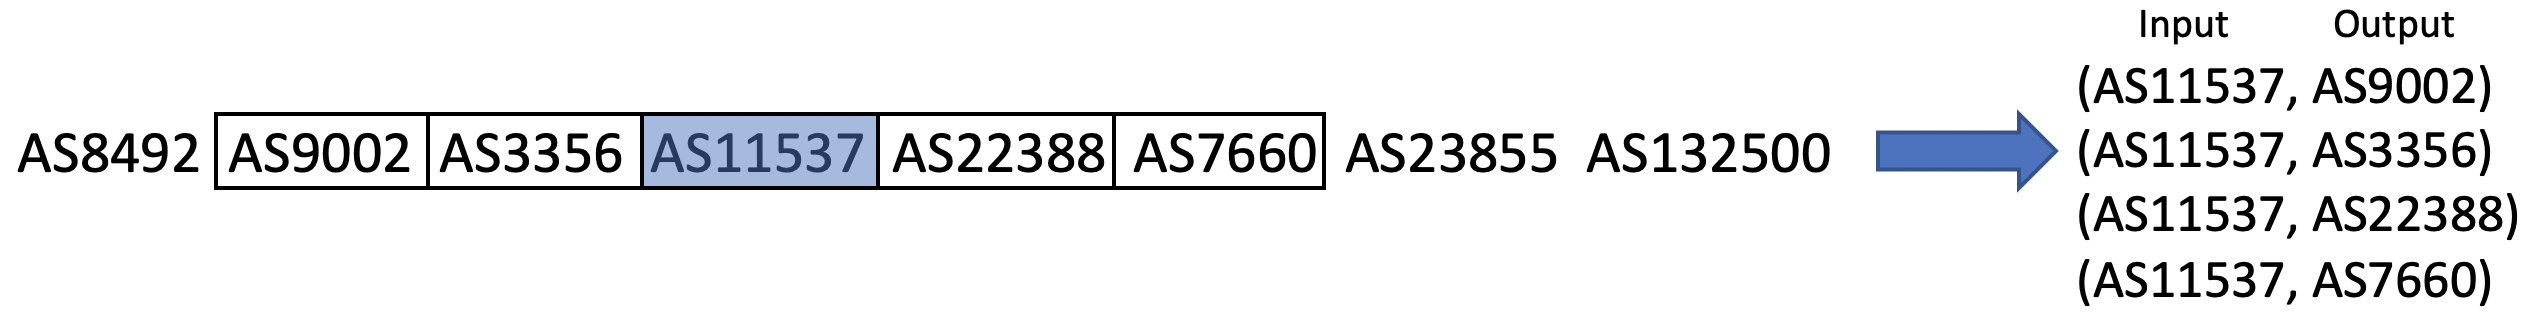
\includegraphics[width=10cm]{img/metodosASRel/BGP2Vec1.png}
    \caption{Proceso de generación de \textit{embeddings} en BGP2Vec a partir de las RIBs utilizando el modelo Skip-gram.}
    \label{fig:BGP2Vec-AS-Path}
\end{figure}

Una vez entrenado los embeddings para cada ASN, se continúa con la tarea de clasificación de las relaciones entre los Sistemas Autónomos. Para esto se ocupa una Red Neuronal Artificial de dos capas.


\begin{figure}[h]
    \centering
    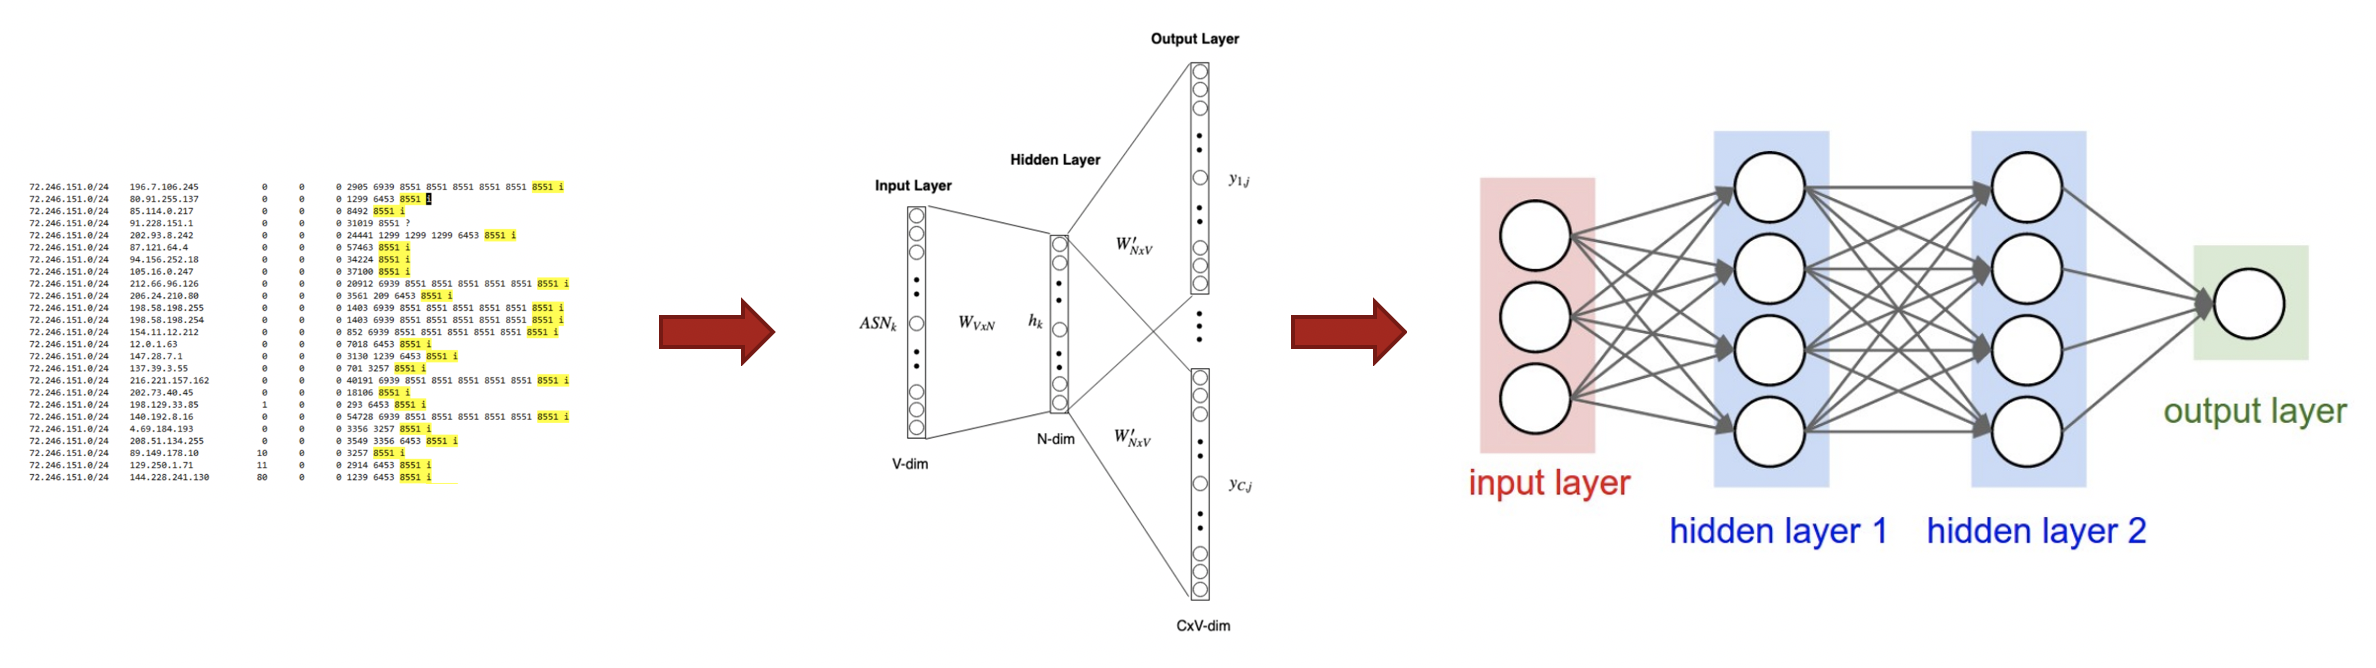
\includegraphics[width=10cm]{img/metodosASRel/BGP2Vec2.png}
    \caption{Pipeline empleada por estudio BGP2Vec para clasificar las relaciones entre Sistemas Autónomos. Primero a partir de RIBs se crean sus \textit{embeddings} y luego una ANN actúa como clasificador.}

    \label{fig:BGP2Vec-Pipeline}
\end{figure}


Para la etapa inicial de entrenamiento de BGP2Vec, se utilizaron anuncios extraídos de RouteViews \cite{RouteViewsProject}, que contenían anuncios de rutas de AS (AS PATH) recolectadas por 19 colectores. Este dataset recopiló 3,600,000 rutas de AS con 62,525 vértices de AS y 113,400 enlaces no dirigidos.

Para el entrenamiento de la Red Neuronal encargada de la clasificación de las relaciones entre ASes, se utilizó el conjunto de datos de relaciones entre AS de CAIDA \cite{CAIDAS-relationship}, que contiene relaciones P2P y P2C/C2P. Además, para algunos experimentos, se empleó el dataset ToR de BGProtect (www.BGProtect.com) \cite{BGProtect}, basado en el trabajo de Shavitt et al. \cite{NearDeterministicInference}.


% https:%github.com/talshapira/BGP2Vec/tree/main
% Se uso este conjunto de datos para entrenar ls red neuronal y varios algoritmos de aprendizaje supervisado basados en embedding de ASN, y como referencia para la comparación con trabajos previos.

% El algoritmo de BGP2Vec se basa en la misma idea de Word2Vec, donde se buscar representar vectorialmente los ASes de manera que las relaciones entre ellos se puedan inferir a partir de la distancia entre los vectores. Para esto, se utilizan los anuncios BGP de rutas de AS (AS PATH) para entrenar un modelo de Deep Learning que genere _embeddings_ de los ASes. Estos _embeddings_ son utilizados para clasificar las relaciones entre los ASes.
% E n este caso s eocupo skip-gram, que es un modelo de aprendizaje no supervisado para aprender representaciones vectoriales de palabras. El objetivo es aprender representaciones vectoriales de palabras que sean útiles para predecir las palabras vecinas en un contexto dado.

% ¿Cómo se creó el Dataset?

% Para este caso se necesitan 2 datasets, el primero el dataset correspondiente a las rutas BGP, para por medio de Word2Vec characterizeembedding
% de los Ases y un segundo dataset para entrenar la red neuronal srtificial para la tarea de clasificacion.
 
% 1. A partir del dataset de rutas BGP proporcionadas por CAIDA \cite{CAIDAS-relationship}, para el caso especifico de este problema _aaaammdd.as-rel2.txt.bz2_ correspondiente a la fecha dd/mm/aaaa, se generaron dos listas: una con pares de Sistemas Autónomos que comparten algún tipo de relación, y otra que etiqueta el tipo de la relación de cada par.

% % TODO: Agregar fecha dataset 

% ```python
% tor_dataset = []
% tor_labels = []

% with bz2.open(DATA_PATH + ToR_CSV, "rt") as csv_file:
%     reader = csv.reader(csv_file,delimiter='|')
%     for i, row in enumerate(reader):
%       if row[0][0] != '#' and int(row[2]) in TOR_CSV_LABELS_DICT.values():
%         # print(row)
%         # Agrego arista en ambos sentidos 
%         tor_dataset.append(np.asarray(row[:2]))
%         tor_dataset.append(np.asarray(row[1::-1]))

%         # Si etiqueta -1 -> 2; si etiqueta 0 -> 0; si etiqueta 1 -> 1
%         label = int(row[2])
%         if label == -1:         # Si es P2C,
%           label = 2
%           tor_labels += [label, 1]
%         elif label == 0:        # Si es P2P
%           tor_labels += [label, label]
%         else:                   # Si es C2P
%           tor_labels += [label,2]
% ```
% Estas listas se gurdan en archivos np con los nombres _bgp2vec_caida_tor_dataset.npy_ y _bgp2vec_caida_tor_labels.npy_ respectivamente.

% Las etiquetas correspondientes a las relaciones entre ASes corresponden a:
% - 0: Peer-to-Peer (P2P)
% - 1: Customer-to-Provider (C2P)
% - 2: Provider-to-Customer (P2C)
% Con un conteo de 619648, 121096 y 121096 relaciones, respectivamente.

% 2. Crear 



% 3. Se entrena  el modelo BGP2VEC con el dataset de rutas BGP y se guarda el modelo en el archivo _bgp2vec.word2vec_.

% ```python
% test_limit = 2000000 #cantidad paths/horaciones
% mode = None# 'test' # par limitar cantidad de paths/oraciones
% epochs = 1
% debug = True


% # Crea embeddings de ASN con  BGP2VEC y lo guarda en "bgp2vec/bgp2vec.word2vec"
% bgp2vec = BGP2VEC(model_path = MODELS_PATH ,oix_path=oix_path,rewrite=True, test_limit= test_limit, mode = mode, epochs = epochs)

% ```

% 4. 




\subsubsection{ProbLink} \label{sec:anexo_problink}




ProbLink es un algoritmo probabilístico para inferir las relaciones entre Sistemas Autónomos propuesto por Yuchen Jin et al. \cite{ProbLink}. 
Este permite el uso de atributos con valores estocásticos. Toma en cuenta información sobre los links y caminos que atraviesan . ProbLink no impone un orden específico en el que los ASes y los enlances deben ser analizados, en su lugar itera con continuamente hasta alcanzar una convergencia. \\

% El algoritmo comienza con la clasificación inicial con los resultados de CoreToLeaf, un algoritmo de clasificación de relaciones entre ASes propuesto por los mismos autores de baja complejidad. Si CoreToLeaf etiqueta el link $L$ como un link P2C, entonces $P(L=P2P) = 0.0$, $P(L=C2P)= 0.0$ y $P(L=P2C)=1.0$.

Para cada atributo se calcula la distribución de probabilidad condicional basada en los datos observados y el conjunto inicial de etiquetas.
Luego en cada iteración, se actualiza las probabilidades de los tipos de cada enlace ejecutando su algoritmo probabilistico y se recalcula las distribuciones de las caracteristicas utilizando los valores de probabilidad actualizadas de cada enlace. 
Se repite el proceso hasta la convergencia, es decir , hasta que el porcentaje de enlaces que cambia de etiqueta caiga por debajo de un umbral.\\

Las características utilizadas para calcular la probabilidad de cada relación son:
\begin{itemize}
    \item \textbf{Atributo Triplet:} Analiza secuencias de tres enlaces en una ruta BGP y modela la \textit{valley-freeness} de manera probabilística.
    \item \textbf{Atributo Non-path:} Mide la probabilidad de que un enlace tenga enlaces adyacentes p2p o p2c que no aparezcan antes en ninguna ruta. Captura la propiedad de que un enlace es menos probable que sea p2c si tiene muchos enlaces adyacentes p2p/p2c sin aparecer previamente en las rutas.
    \item \textbf{Atributo Distance to clique:} Identifica que los ASes de alto nivel están más cerca entre sí en términos de saltos AS y que estos suelen actuar como proveedores, mientras que los ASes de bajo nivel tienden a ser peers.
    \item \textbf{Atributo Vantage point:} El número de puntos de vista (VPs) que observan un enlace puede indicar su tipo. Se basa en la suposición de que los enlaces p2c son más propensos a ser observados por múltiples VPs en comparación con los enlaces p2p y c2p.
    \item \textbf{Atributo Co-located IXP and co-located private peering facility:} Usa datos de PeeringDB para identificar ASes que comparten IXPs o instalaciones, lo que sugiere una mayor probabilidad de que estén en una relación de peering.

\end{itemize}

\subsection{Toposcope} \label{sec:toposcope}

En 2018, Jiajun Zhang y otros investigadores propusieron \textit{Toposcope} \cite{Toposcope}, un método diseñado para inferir relaciones entre Sistemas Autónomos a gran escala a partir de datos de BGP. A diferencia de enfoques heurísticos clásicos como los de Gao o Ruan, Toposcope combina múltiples fuentes de información y utiliza un modelo probabilístico que busca maximizar la consistencia global de las relaciones inferidas.\\

El objetivo central de Toposcope es construir un grafo dirigido de relaciones AS que respete lo mejor posible la estructura real de la red de Internet, reduciendo las inconsistencias que surgen al aplicar reglas locales estrictas (como la propiedad \textit{valley-free}). Para ello, formula la inferencia de relaciones como un problema de optimización global.\\

El algoritmo propuesto se basa en tres componentes principales:
\begin{enumerate}
    \item \textbf{Recopilación de datos:} Utiliza RIBs y anuncios de BGP obtenidos de RouteViews y RIPE RIS como entrada principal.
    \item \textbf{Modelo probabilístico de relaciones:} Define una función de probabilidad sobre las posibles asignaciones de relaciones (P2C, C2P, P2P) en el grafo de ASes, penalizando aquellas configuraciones que violen con frecuencia la regla \textit{valley-free}.
    \item \textbf{Optimización global:} Emplea un proceso iterativo para ajustar las relaciones de los enlaces de AS, de manera que se maximice la probabilidad total del grafo bajo el modelo definido.
\end{enumerate}


%\subsection{ AS-Rank Algorithm}
%El algoritmo AS-Rank tine lso soguientes pasos:
%\begin{enumerate}
   % \item Limpiar y descartar rutas con irregularidades.
   % \item Ordenar los ASes en orden decreciente en base al grado y grado de transito calculado.
  %  \item Inferir un clique libre de tránsito (es decir, AS de nivel 1) en la parte superior de la jerarquía de AS y etiquetar los enlaces entre cada par de AS en el clique como enlaces punto a punto (p2p).
 %   \item Eliminar rutas contaminadas.
 %   \item Visitar los AS en el orden del ranking en (2) y etiquetar un enlace como c2p si su enlace anterior en una ruta BGP está compuesto por dos miembros del clique, o si su enlace anterior en una ruta BGP ya está etiquetado como c2p.
%    \item Inferir relaciones c2p a partir de los puntos de vista (VP) que se infiere están anunciando rutas sin rutas de proveedor.
    
%\end{enumerate}

%\subsection{AS-Rank Clique Inference}



%El calculo del clique se realiza de al siguiente manera:

%\begin{enumerate}
%    \item Encontrar los 10 AS principales por grado de tránsito.
%    \item Si hay tres miembros consecutivos (X-Y-Z) entre los 10 AS principales que aparecen en las rutas, y hay más de 5 AS descendentes desde X-Y-Z (para asegurarse de que las rutas que contienen tres miembros consecutivos no estén contaminadas), desconectar el enlace entre X y Z, aunque X y Z estén conectados en algunas rutas.
%    \item Encontrar el clique más grande en términos de la suma del grado de tránsito entre los 10 AS principales, denotado como C.
%    \item Visitar los demás AS de arriba hacia abajo según el grado de tránsito, añadir un AS Z a C si Z tiene enlaces con todos los miembros de C.
%    \item De manera similar al paso 2: Si hay tres miembros consecutivos (X-Y-Z) en C que aparecen en las rutas, y hay más de 5 AS descendentes desde X-Y-Z, desconectar el enlace entre X y Z.
%    \item Encontrar el clique más grande en C en términos de la suma del grado de tránsito como el clique final inferido.
%\end{enumerate}



% == Desafíos en la inferencia de Relaciones entre Sistemas Autónomos
% - Muchoas tecnicas de inferencia de relaciones entre AS relaizan 3 suposiciones-.
%   1. Highest degree ASes sit at top of the routing hierarchy
%   2. Peering ASes have similar degree
%   3. Providers have larger degree than customers
% \cite{InferringASRelatioships2001} \cite{InferringASRelationshipsDeadEndorLivelyBeginning}
% esto afecta la accuracy de los algormios ya  que un paso impoortante de stos es encontrar/identificar ql clique Tier 1 Ases al top de la jerarquía.
% Debido al fenomeno de "flattening of the internet" [he flattening
% internet topology: Natural evolution, unsightly barna-
% cles or contrived collapse?] sabemos que Large content providers como Google, Microsoft y otros los cuales tineen un numero alto de degree are more willing to peer with large number  of lower tier Ases to get free and more efficient traffic exchange. 
% % TODO: buscar más de esto

% - violacion de la property Valley-free , que son la causa principal de inferir p2c links y conflictos. 3% of the BGP Paths violate valley-free property in AS-Rank segun \cite{ProbLink} en su estidio , la cual policias de AS que usan unconventional economic models [alley-free violation in inter-
% net routinganalysis based on BGP community data. In
% Communications (ICC)]. Por lo que un algoritmo robusto debiese tomar encuenta todos los path que pasan por ese link. y podría tener q revisitar y update la inferencia hehca por un  después de inferir los tipos de los links vecinos.
% % TODO: leer papaer

% - Current technics are Sensitive to VP and Snapshot Selection: \cite{probabilidad} encontro que hay una variación alta de la accuracy cuando esta fue apluciada a AS-Rank algorimo para snapshops de los BGP Path de forma consecutiva. }en el fonod por el paso 1 

% TODO: Agregar que a diferencia d eotros algoritmos que unicamente ocupaabn los bgp update so ribs, este tmb otra otros datos como .....

% == EXTRAS

% Estudios hechos por Yuchenjin et al. \cite{ProbLink} dentro de su estudio en la creación de un algoritmo de inferencias de ASes, determinó 5 tipos de links que eran dificiles de inferir. Para esto ocupo CoreToLeaf un algoritmo basico de inferencia el cual solo ocupaba la asumtio of valley-free y la ubicacion de Top provider AS para determinar las relaciones(mas info en  la seccion de ProbLink):


% ToR information allows us to infer the possible routes selected by BGP, e.g., 
% in case of a link failure \cite{Internet-resiliency-to-attacks-and-failures-under-BGP-policy-routing},

% It can also be used to identify malicious fiddling with the routing system,
% known as IP hijack attack \cite{Chinas-Maxim-Leave-No-Access-Point-Unexploited-The-Hidden}

% BGP allows each AS to choose its own administrative policy in selecting routes and propagating reachability information to others.\cite{InferringASRelatioships2001} 




% - Congestión en la red \cite{InferringPersistentInterdomainCongestion}
% - Detección de Sistemas Autónomos (ASes) maliciosos [51, 23]
% - La implementación de mecanismos de seguridad para BGP [22]
% - La protección del anonimato de los datos [72]
% - La optimización de la transmisión de video [31] 


% \subsection{Word2vec} \label{sec:word2vec_anexo}

% Primero es necesario entender el significado de \textit{Word Embedding}, la cual se refiere a una representación vectorial que captura el significado y contexto de una palabra en un espacio vectorial de varias dimensiones. De esta forma, es posible representar también la similitud semántica y sintáctica entre las palabra.\\

% \textbf{¿Cómo funciona word2vec?}

% Existen dos enfoques de Word2vec, ambas basadas en Redes Neuronal:

% \begin{itemize}
%     \item \textbf{Continuous Bag of Words (CBOW)}: El modelo recibe como entrada el contexto (palabras vecinas) e intenta predecir la palabra objetivo. La salida de esta Red corresponde a la nueva representación vectorial de dicha palabra.
%     \item \textbf{Skip-gram}: El modelo recibe como entrada la palabra objetivo y predice las palabras del contexto. La salida de la Red es la representación vectorial de la palabra.    
% \end{itemize}


%\section{Reducción de dimensionalidad} \label{sec:Reduccion_dimensionalidad}

%Con el fin de poder visualizar y analizar propiedades de los \textit{embeddings} generados por las tareas de los modelos, se puede aplicar diferentes técnicas de reducción de dimensionalidad. Esto para poder graficar vectores de alta dimensión en un espacio bidimensional o tridimensional, facilitando así su interpretación visual, distribución y agrupamiento. Dentro de los métodos encontramos:\\

%\begin{itemize}
%    \item \textbf{PCA (Principal Component Analysis):} método lineal que conserva la mayor varianza posible de los datos originales. Se usó como primera aproximación para observar la dispersión global de los embeddings.
 %   \item \textbf{t-SNE (t-distributed Stochastic Neighbor Embedding):} técnica no lineal orientada a preservar las relaciones locales entre los puntos, útil para detectar agrupamientos o comunidades.
    %\item \textbf{UMAP (Uniform Manifold Approximation and Projection):} técnica más reciente que preserva tanto la estructura local como global del espacio de características, con menor costo computacional que t-SNE.
%\end{itemize}

%Los \textit{embeddings} fueron reducidos desde una dimensionalidad de $d=32$ a $d=2$, con el objetivo de visualizar y analizar patrones en el agrupamiento de los Sistemas Autónomos (ASes) según su tipo de relación (p2p, c2p, p2c).\\



\subsubsection{TopoScope} \label{sec:anexo_toposcope}




	% \input{Anexos/03Anexo_Fundamentos_ML_GNNs.tex}
	% \input{Anexos/04Anexo_Analisis_Exploratorio.tex}
	% \input{Anexos/05Anexo_Configuracion_Experimentos.tex}

\appendix

% \section{Fundamentos de Internet y BGP}
% \subsection{Internet}
% \subsection{Sistemas Autónomos}
% \subsection{Internet Exchange Points}
% \subsection{Ruteo en Internet}
% \subsubsection{Ruteo interno}
% \subsubsection{Ruteo externo}
% \subsection{Protocolo BGP}
% \subsubsection{Funcionamiento general}
% \subsubsection{Mensajes BGP}
% \subsubsection{Atributos BGP}
% \subsubsection{Routing Information Base (RIB)}
% \subsubsection{Colectores y vantage points}
% \subsection{Topología de Internet}
% \subsubsection{Topología de Internet a diferentes niveles}
% \subsubsection{Topología de Internet a nivel de Sistemas Autónomos}
% \subsection{Recolección de datos de Internet}
% \subsubsection{CAIDA}
% \subsubsection{RouteViews Project}
% \subsubsection{RIPE RIS}
% \subsubsection{PeeringDB}
% \subsection{Construcción del grafo a partir de datos BGP}

% \subsection{Inferencia de relaciones entre Sistemas Autónomos}
% \subsection{Relaciones económicas entre Sistemas Autónomos}
% \subsection{Tipos de relaciones entre AS}
% \subsection{Valley-Free Routing}
% \subsection{Problema de inferencia de relaciones}
% \subsection{Métodos de inferencia basados en heurísticas}
% \subsubsection{Gao}
% \subsubsection{LU Rank}
% \subsection{Métodos basados en aprendizaje automático}
% \subsubsection{BGP2Vec}
% \subsubsection{ProbLink}
% \subsubsection{TopoScope}

% \subsection{Fundamentos de aprendizaje automático}
% \subsection{Inteligencia Artificial}
% \subsection{Machine Learning}
% \subsection{Representaciones y embeddings}
% \subsection{Evaluación de modelos}

% \subsection{Redes neuronales}
% \subsection{Redes neuronales artificiales}
% \subsection{Perceptrón o neurona artificial}
% \subsection{Redes neuronales feed-forward}
% \subsection{Funciones de activación}
% \subsection{Entrenamiento de redes neuronales}
% \subsection{Backpropagation}
% \subsection{Redes neuronales convolucionales}

% \section{Redes neuronales de grafos}
% \section{Teoría de grafos}
% \subsection{Definición de grafo}
% \subsection{Representación de grafos}
% \subsection{Tipos de grafos}
% \section{Aprendizaje en grafos}
% \section{Redes neuronales de grafos}
% \section{Message Passing}
% \section{Embeddings de nodos}
% \section{Tareas de aprendizaje sobre grafos}
% \section{Arquitecturas de GNN}
% \subsection{Message Passing Neural Networks (MPNN)}
% \subsection{Graph Convolutional Networks (GCN)}
% \subsection{Graph Attention Networks (GAT)}
% \subsection{GraphSAGE}

% \section{Análisis exploratorio y características del dataset}
% \subsection{Exploración de datos de PeeringDB}
% \subsection{Exploración de la tabla \texttt{net}}
% \subsection{Exploración de Internet Exchange Points}
% \subsection{Atributos utilizados para los Sistemas Autónomos}
% \subsection{Análisis de atributos de PeeringDB}
% \subsubsection{Atributos numéricos}
% \subsubsection{Atributos categóricos}
% \subsubsection{Implicancias para el preprocesamiento y el modelado}
% \subsection{Análisis del grafo construido}
% \subsection{Distribución del grado de los AS}
% \subsection{Comparación temporal de rutas BGP}
% \subsection{Lista de Sistemas Autónomos Tier-1 considerados}
% \subsection{Tablas de colectores disponibles}

% \section{Configuración experimental}
% \subsection{Arquitecturas evaluadas}
% \subsection{Hiperparámetros}
% \subsection{Configuración de entrenamiento}
% \subsection{Métricas de evaluación}
% \subsection{Hardware y entorno de ejecución}





	% 1) Fundamentos de Internet y contexto conceptual
	\section{Fundamentos de Internet y BGP} \label{sec:anexo_fundamentos_internet_bgp}


\subsection{Internet} \label{sec:anexo_internet}

Internet es una red global compuesta por múltiples redes interconectadas entre sí, que permite la comunicación y el intercambio de información entre dispositivos distribuidos geográficamente. 
Su funcionamiento depende de la cooperación entre distintos sistemas de comunicación, protocolos y organizaciones que administran diferentes segmentos de la red. 
Gracias a esta infraestructura, es posible ofrecer servicios como navegación web, correo electrónico, transmisión de contenido y múltiples aplicaciones distribuidas.\\


Desde una perspectiva estructural, Internet puede entenderse como una \textbf{red de redes}, donde distintos dominios administrativos se conectan para permitir conectividad global. 
Esta característica la convierte en un sistema distribuido de gran escala, dinámico y heterogéneo, en el cual la información puede viajar a través de múltiples caminos antes de 
alcanzar su destino final. Debido a esto una buen amanera de abstrar su funcionamiento y complejidad para su estudio es abstraer su estructura a una reprsenatcion en forma de grafo.\\


El correcto funcionamiento de Internet depende de la cooperación entre las diferentes partes que lo forma,es por esto que existe una jerarquia de organizaciones encargadas de coordinar los recursos y estándares. En particular, la \textbf{IANA} (\textit{Internet Assigned Numbers Authority}) 
administra globalmente recursos críticos como bloques de direcciones IP y números de Sistemas Autónomos. Estos recursos son luego distribuidos por los \textbf{Registros Regionales de Internet} 
(\textit{Regional Internet Registries}, \textbf{RIRs}), entre los que se encuentran \textbf{ARIN}, \textbf{RIPE NCC}, \textbf{APNIC}, \textbf{LACNIC} y \textbf{AFRINIC}, cada uno responsable 
de una región específica del mundo.
Asimismo, organizaciones como la \textbf{IETF} (\textit{Internet Engineering Task Force}) definen los estándares técnicos que permiten la interoperabilidad de Internet, incluyendo protocolos 
fundamentales como TCP/IP, DNS y BGP. Por su parte, la \textbf{ICANN} (\textit{Internet Corporation for Assigned Names and Numbers}) coordina el sistema global de nombres de dominio y participa 
en la administración de recursos de numeración a nivel internacional. Finalmente, los \textbf{Proveedores de Servicios de Internet} (\textit{Internet Service Providers}, \textbf{ISPs}) desempeñan 
un rol central al proporcionar conectividad a usuarios, empresas y otras redes, enlazando la operación de estas entidades con la infraestructura efectiva de Internet.\\


% \begin{figure}[H]
%     \centering
%     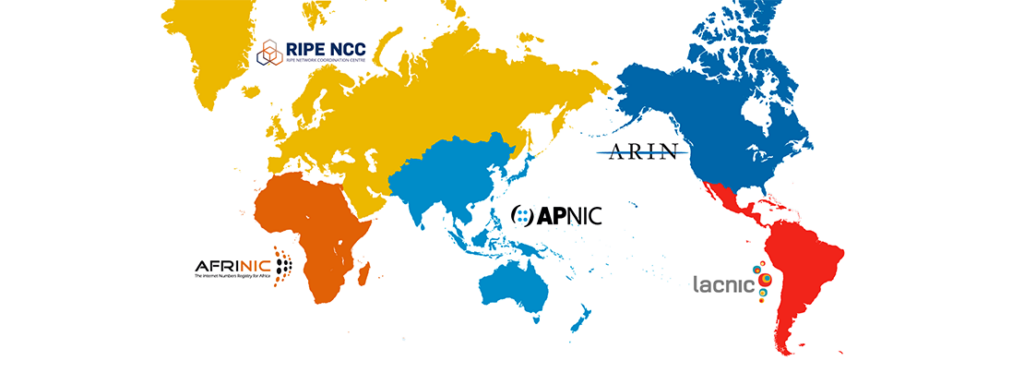
\includegraphics[width=0.6\textwidth]{Anexos/img/01/RIRs.png}
%     \caption{RIRs y su cobertura geográfica. Fuente: https://blog.apnic.net/2024/10/28/revising-the-criteria-for-the-accreditation-of-rirs/}
%     \label{fig:rirs_map}
% \end{figure}

\subsection{Sistemas Autónomos} \label{sec:anexo_sistemas_autonomos}


Como se habló previamente en la Sección~\ref{sec:sistemas_autonomos}, los \textbf{Sistemas Autónomos (AS)} son un conjunto de dispositivos que comparten un mismo protocolo de ruteo y son administrados por una misma entidad u organización, como proveedores de servicios de Internet (ISP), universidades, empresas o instituciones gubernamentales. 
La interconexión entre estos sistemas es la que da lugar a la estructura global de \textbf{Internet}.\\


Cada AS se identifica mediante un \textbf{Número de Sistema Autónomo} (\textit{Autonomous System Number}, \textbf{ASN}) que permite distinguirlo dentro del ecosistema de Internet. 
Además, cada AS administra o anuncia uno o más bloques de direcciones \textbf{IP}, los cuales son asignados por los \textbf{Registros Regionales de Internet} (\textit{Regional Internet Registries}, \textbf{RIRs}) , a partir de bloques delegados por la \textbf{Autoridad de Asignación de Números de Internet} (\textit{Internet Assigned Numbers Authority}, \textbf{IANA}).
En este proceso, los RIRs distribuyen recursos a los \textbf{Registros Locales de Internet} (\textit{Local Internet Registries}, \textbf{LIRs}), proveedores y usuarios finales.\\

Los ASNs pueden clasificarse en \textbf{públicos} o \textbf{privados}. 
Los \textbf{ASN públicos} son asignados por los RIRs y son únicos a nivel global, por lo que pueden aparecer en las tablas de enrutamiento públicas de Internet. 
En cambio, los \textbf{ASN privados} se utilizan en entornos internos, pruebas, simulaciones o conexiones cerradas entre routers, y no deben propagarse hacia la tabla global de Internet. 
Entre los rangos reservados para uso privado se encuentran 64512--65534 y 4200000000--4294967294 y estos estan indicados en el RFC 6996.\\ %TODO: citar

Desde el punto de vista de su rol dentro de la topología de Internet, los ASes suelen clasificarse en distintos niveles jerárquicos. 
Una clasificación ampliamente utilizada distingue entre \textbf{Tier-1}, \textbf{Tier-2} y \textbf{Tier-3}. 
Los ASes \textbf{Tier-1} corresponden a grandes proveedores globales de tránsito que conforman el \textit{backbone} de Internet y que intercambian tráfico entre sí sin pagar tránsito. 
Los \textbf{Tier-2} suelen corresponder a operadores regionales o nacionales que compran tránsito a redes Tier-1 y, a su vez, venden tránsito a redes de menor escala. 
Finalmente, los \textbf{Tier-3} suelen ser proveedores locales o redes de acceso que pagan por tránsito para ofrecer conectividad a usuarios finales~\cite{InterconnectionPeeringSettlements}.\\

Otra forma de caracterizar la posición de un AS dentro de Internet es mediante su \textit{customer cone}, es decir, el conjunto de ASes que puede alcanzar a través de relaciones proveedor--cliente. 
En este contexto, Luckie \textit{et al.}~\cite{ASRank} utilizan esta noción para estimar el grado de globalidad de un AS y su posición relativa en la jerarquía de Internet.
Si el \textit{customer cone} es mayor o igual a 200, se considera Tier-1, si es mayor a 2,000, se considera Tier-2 y si es menor a 200, se considera Tier-3.\\


Además de esta clasificación jerárquica, los Sistemas Autónomos pueden distinguirse según el número y tipo de conexiones externas que mantienen. 
En este contexto, un AS puede ser clasificado como:

\begin{itemize}
    \item \textbf{Stub AS}: se conecta únicamente a otro Sistema Autónomo y no transporta tráfico de tránsito para terceros.
    \item \textbf{Transit AS}: se conecta a múltiples Sistemas Autónomos y permite el tránsito de tráfico entre ellos.
    \item \textbf{Multihomed AS}: se conecta a más de un Sistema Autónomo para mejorar redundancia o disponibilidad, pero no ofrece tránsito entre ellos.
\end{itemize}

De manera relacionada, también es común distinguir entre ASes \textbf{\textit{single-homed}} y \textbf{\textit{multi-homed}}. 
Los primeros poseen una única conexión hacia otro AS, mientras que los segundos tienen conexiones hacia dos o más ASes. 
Esta distinción es importante, ya que influye en la resiliencia, redundancia y diversidad de rutas disponibles para una red.\\



En el contexto del enrutamiento interdominio también aparecen los conceptos de \textbf{\textit{upstream}} y \textbf{\textit{downstream}}. 
Un \textit{upstream} corresponde, en términos generales, al proveedor o red ubicada ``hacia arriba'' en la cadena de conectividad, es decir, 
aquella de la cual un AS obtiene tránsito hacia Internet. 
Por el contrario, un \textit{downstream} corresponde a las redes o clientes que dependen de un AS para alcanzar otros destinos en Internet. 
Esta relación es especialmente importante al estudiar políticas de exportación de rutas y relaciones económicas entre ASes.\\

Otro concepto relevante es el de \textbf{Multi-Origin AS} (\textbf{MOAS}), que ocurre cuando un mismo prefijo IP es anunciado por múltiples 
Sistemas Autónomos como origen. Esta situación puede producirse por distintas razones. Por ejemplo, en despliegues de \textit{anycast}, donde un 
mismo prefijo se anuncia desde múltiples ubicaciones para acercar un servicio al usuario final; durante procesos de migración o transición entre 
proveedores; en escenarios de \textit{multihoming}; o bien debido a errores de configuración. En casos más críticos, la presencia de MOAS también 
puede asociarse a conflictos de origen, secuestro de prefijos (\textit{prefix hijacking}) o \textit{route leaks}. Por esta razón, su identificación 
es relevante para el análisis del comportamiento del protocolo BGP y la estabilidad del enrutamiento.\\

Finalmente, algunos ejemplos de Sistemas Autónomos ampliamente conocidos son \textbf{AS15169}, asociado a Google, y \textbf{AS3356}, correspondiente 
a Lumen/Level 3. En contraste, identificadores como \textbf{AS65001} suelen utilizarse en entornos privados, de laboratorio o simulación.

% TODO: Agregar!!!
% Esta jerarquía, sin embargo, se ha vuelto más compleja con la aparición de grandes proveedores de contenido, CDNs y operadores cloud con infraestructura propia.


\subsection{Internet Exchange Points} \label{sec:anexo_internet_exchange_points}
Los \textit{Internet Exchange Points} (IXPs) son puntos de interconexión donde múltiples ASes pueden establecer relaciones de peering con otros ASes \cite{Computer-Networking}.\\

Un IXP consiste generalmente en un switch  o router de alta velocidad y capacidad que conecta routers de diferentes ASes, permitiendo el intercambio directo de tráfico sin necesidad 
de atravesar redes intermedias. Mejorando así el intercambio de tráfico, haciéndolo más eficiente y de bajo costo.\\

% FIXME: arregalr redaccion
Las relaciones de tráfico en un IXP se establecen mediante el protocolo BGP, y el IXP solo actua como un intermediario. 
De esta forma por ejemplo un ISP en vez de estar conectados a multiples ASes  en una coneccion punto a punto, puede conectarse 
unicamente al IXP y como estos otros ASess tambien estaran conectados al IXP se ahorra recuersos fisicos y de administracion.\\

Al igual que los ASes, los IXPs tienen un ASN. Sin embargo, de forma generalizada, este ASN se extrae de los AS PATH en BGP. 
Algunos IXPs lo mantienen visible como método de debugging \cite{InferringASRelatioships2001}. 


\subsection{Ruteo} \label{sec:anexo_ruteo}


El ruteo consiste en la elección de caminos que seguirá un paquete dentro de una red, con
el propósito de garantizar que la información que se transmite por Internet pueda llegar a
su destino mediante la ruta más eficiente. Una red está formada por múltiples maquinas a
las cuales se les llama nodo y las rutas que las unen. La comunicación entre dos nodos de
la red se puede establecer mediante la interconexión de diferentes caminos, permitiendo así,
conectar dos nodos que no tienen una conexión directa por medio de nodos intermedios. De
esta forma el enrutamiento es el proceso de seleccionar la mejor ruta entre estos nodos en
base a algún parámetro o reglas.\\

Un enrutador o router es un dispositivo de red que se conecta a otros dispositivos y redes.
Son los encargados de seleccionar las rutas que irán tomando los datos enviados.\\

El ruteo opera gracias a las tablas de rutas presentes en los routers y a la información
proporcionada en los encabezados de los paquetes, los cuales contienen datos sobre el destino
del paquete. Cuando llega un paquete a un router, se consulta ls tabla de enrutamiento para
localizar la dirección destinos, y posteriormente dirigir el paquete al próximo router o punto
de red.\\

Existen dos tipos de enrutamiento: estático y dinámico. El enrutamiento estático implica
el uso de tablas estáticas, las cuales deben ser modificadas manualmente para cambiar su
configuración. Es útil en situaciones donde los parámetros de red permanecen constantes.
Por otro lado, en el enrutamiento dinámico, los routers se encargan de ir actualizando las
tablas de enrutamiento en tiempo real, ajustándolas según las condiciones de la red. Este
proceso se lleva a cabo mediante los protocolos de enrutamiento.\\





\subsubsection{Ruteo interno} \label{sec:anexo_ruteo_interno}

El ruteo interno, también llamado \textit{intra-domain routing}, se encarga de gestionar las 
rutas a seguir de un paquete dentro de un Sistema Autónomo.
En este contexto los routers ocupan protocolos de enrutamiento interno para intercambiar la
información del estado de la red y las rutas disponibles. Entre los protocolos de ruteo interno
se tiene:
\begin{itemize}
    \item OSPF (Open Shortest Path First): Utiliza el algoritmo de Dijkstra para determinar las
rutas más cortas entre nodos\cite{RFC-OSPF}.
    \item RIP (Routing Information Protocol): Utiliza un enfoque de vector de distancia para
calcular la ruta más optima, basándose en la cantidad de saltos\cite{RFC-RIP}.
\end{itemize} 


\subsubsection{Ruteo externo} \label{sec:anexo_ruteo_externo}


Se centra en la gestión de rutas entre los diferentes Sistemas Autónomos que conforman
el Internet. En este caso, se usan protocolos de enrutamiento externo, que al igual que los
protocolos de enrutamiento interno se encarga de intercambiar la información de las rutas
disponibles, permitiendo así­ que paquetes viajen de manera más efectiva. Algunos protocolos
de enrutamiento externos son:\\

\begin{itemize}
    \item  BGP (Border Gateway Protocol): Tiene un enfoque de vector de distancia. Utiliza
un enfoque de vector de distancia y toma decisiones basadas en polí­ticas de red para
intercambiar información eficientemente\cite{RFC-BGP}.
    \item IS-IS (Intermediate System to Intermediate System): Protocolo de enrutamiento de
estado de enlace, similar a OSPF\cite{RFC-ISIS}.
\end{itemize} 



\subsection{BGP} \label{sec:anexo_bgp}

El \textit{Border Gateway Protocol} (BGP) es el protocolo de enrutamiento utilizado para 
intercambiar información de rutas entre Sistemas Autónomos en Internet. Su rol es permitir 
que cada AS conozca qué prefijos son alcanzables a través de sus vecinos y qué caminos pueden 
seguirse para llegar a ellos.

BGP es un Protocolo PATH Vector, esto significa que la selección de rutas no depende exclusivamente 
de métricas de distancia, sino también de preferencias definidas localmente por cada Sistema 
Autónomo. Gracias a ello, BGP permite que cada operador controle qué rutas anunciar, cuáles aceptar y cuáles preferir, de acuerdo con sus necesidades técnicas, comerciales o estratégicas.




\subsection{Funcionamiento general}

El funcionamiento de BGP comienza cuando dos routers de borde pertenecientes a ASes distintos establecen 
una sesión de comunicación. Una vez establecida esta sesión, intercambian información sobre los prefijos 
que pueden alcanzar y los caminos asociados a dichos destinos. Esta información se propaga entre ASes 
vecinos, permitiendo construir progresivamente una vista distribuida de la alcanzabilidad de la red.

Cada vez que ocurre un cambio en la topología o en la disponibilidad de una ruta, BGP actualiza la 
información intercambiada mediante anuncios o retiros de rutas. Así, el protocolo mantiene actualizada 
la información de enrutamiento interdominio, permitiendo la adaptación de Internet frente a cambios 
en su estado operativo.



% Tabla de enrutamiento global vs. tabla local


% tabla de enrutamiento global (BGP global routing table) y la tabla de enrutamiento local.
% Cuando hablamos de enrutamiento en Internet, los routers mantienen tablas donde guardan información sobre cómo alcanzar diferentes redes (prefijos IP).
% Hay una tabla global, que contiene todas las rutas anunciadas públicamente en Internet (a nivel BGP).


% Y cada router o AS mantiene su tabla local, que refleja solo las rutas relevantes según sus políticas y acuerdos de interconexión.


\subsubsection{Mensajes BGP}  \label{sec:anexo_mensajes_bgp}

BGP utiliza TCP \cite{RFC793-TCP} como su protocolo de transporte, lo que significa que no necesita preocuparse por la fragmentación de paquetes, la confirmación de recepción (ACK), la retransmisión de datos, entre otros aspectos de confiabilidad.\\

Los mensajes BGP solo son procesados una vez que han sido completamente recibidos. Su tamaño mínimo es de 19 octetos, correspondiente al HEADER, mientras que el tamaño máximo es de 4096 octetos. Existen 4 tipos de mensajes en BGP: OPEN, UPDATE, KEEPALIVE y NOTIFICATION.\\


\paragraph{Mensaje OPEN}


Luego de establecida la conexión TCP entre los pares BGP, el primer mensaje que se envía en un mensaje OPEN ,mediante 
el cual ambos lados confirman los parámetros de la conexión.
En este mensaje se especifica la versión de BGP a utilizar, el número de Sistema Autónomo (AS) del emisor, el Hold Time, 
el BGP identifier y los parámetros opcionales.
El Hold Time define el tiempo máximo que puede pasar sin recibir un mensaje KEEPALIVE o UPDATE en una sesión antes de que 
la conexión sea cerrada.\\



\paragraph{Mensaje UPDATE}

Se utiliza para transferir información de enrutamiento entre los pares BGP. A través de este mensaje se 
anuncian nuevas rutas y se notifican los withdrawals de aquellas que ya no son válidas.
Además, estos mensajes incluyen path attributes, los cuales proporcionan información sobre las rutas que 
se están anunciando para que luego cada AS pueda decidir la mejor ruta a los diferentes destinos. 
Algunos ejemplos de estos atributos son ORIGIN, AS\_PATH, NEXT\_HOP, MULTI\_EXIT\_DISC, LOCAL\_PREF, ATOMIC\_AGGREGATE y AGGREGATOR.\\



\paragraph{Mensaje KEEPALIVE} 

El intercambio de mensajes KEEPALIVE dentro del protocolo BGP se utiliza para confirmar que la conexión 
entre ambos pares sigue activa, evitando que el Hold Time expire.
Este mensaje consta Unicamente del HEADER de un mensaje BGP, donde se indica que corresponde a un KEEPALIVE 

por medio del campo \textit{type}, cuyo valor es 2, el cual corresponde al valor 2. Dicho mensaje tiene un 
tamaño de 19 octetos.\\


\paragraph{Mensaje NOTIFICATION}

El mensaje \textit{NOTIFICATION} se envía cuando se detecta un error en la comunicación BGP. Una vez enviado, la conexión se cierra.
Este mensaje incluye un código de error y un subcódigo de error, los cuales indican en qué tipo de mensaje se produjo el error y la zona específica del problema. 
Además, contiene un campo de datos que proporciona información adicional sobre el error detectado.\\




\subsection{Colectores y vantage points}


La observación de datos BGP a gran escala se realiza habitualmente mediante colectores, es decir, sistemas que reciben y almacenan anuncios de rutas desde múltiples routers distribuidos en distintos puntos de la red. Cada punto desde el cual se observa la información puede entenderse como un \textit{vantage point}, y la combinación de estos puntos permite construir una vista parcial de la topología global.

Sin embargo, es importante destacar que la información recolectada por estos sistemas no representa una visión completa de Internet. La visibilidad depende de la ubicación y cantidad de los vantage points disponibles, por lo que ciertas conexiones o rutas pueden no ser observadas. Esta limitación debe ser considerada al analizar cualquier grafo construido a partir de datos BGP públicos.



\subsection{Topología de Internet}\label{}

La topología de Internet puede estudiarse a distintos niveles de abstracción, dependiendo de la granularidad con la que se quiera modelar la red. 
En algunos casos interesa analizar conexiones entre interfaces IP, en otros entre routers, puntos de presencia o Sistemas Autónomos completos. Cada uno de estos niveles ofrece una perspectiva distinta sobre la estructura y el funcionamiento de Internet.

En este trabajo, la topología se estudia a nivel de Sistemas Autónomos, ya que este nivel resulta especialmente adecuado para analizar el problema de inferencia de relaciones económicas entre redes. A este nivel, la red puede representarse naturalmente como un grafo cuyos nodos son ASes y cuyas aristas representan conexiones observadas a partir de rutas BGP.

\subsubsection{Topología de Internet a diferentes niveles}

La topología de Internet puede representarse al menos en cuatro niveles principales: nivel IP, donde los nodos corresponden a direcciones o interfaces; nivel router, donde se modelan dispositivos de enrutamiento; nivel PoP, donde se agrupan infraestructuras de presencia geográfica; y nivel AS, donde cada nodo representa un Sistema Autónomo.

Cada uno de estos niveles es útil para distintos fines analíticos. Sin embargo, cuando el interés se centra en la estructura interdominio, los acuerdos de interconexión y las políticas de ruteo entre redes, la representación a nivel de Sistemas Autónomos resulta la más apropiada. Por esta razón, esta tesis adopta la topología AS-level como base para el análisis y modelado.


\subsectionanum{Topología de Internet a nivel de Sistemas Autónomos}

A nivel de Sistemas Autónomos, Internet puede modelarse como un grafo en el que cada nodo representa un AS y cada arista representa una conexión o relación observada entre dos ASes. Esta representación permite abstraer gran parte de la complejidad interna de cada red y concentrarse en el comportamiento estructural de Internet como sistema interdominio.

La construcción de este grafo se basa en la observación de rutas BGP, específicamente en la secuencia de ASes contenida en los atributos \textit{AS\_PATH}. A partir de estas secuencias es posible identificar pares adyacentes de ASes y construir una topología observada. No obstante, esta representación depende de la cobertura de los colectores disponibles y, por tanto, constituye una aproximación parcial de la topología real.


Zhang et al.~\cite{AS-topology-2004} proponen un método para recolectar la topología de Internet a nivel AS.





\subsection{Recolección de datos de Internet} \label{sec:anexo_recoleccion_datos_internet}


% https:%www.pacnog.org/pacnog17/presentations/MappingTheInternet.pdf

La recopilación de datos de Internet es fundamental para comprender su funcionamiento, identificar 
áreas de mejora y optimizar su infraestructura. La información sobre tráfico, rutas y otros permite 
detectar anomalías, prevenir amenazas y mejorar el rendimiento global. Además, estos datos son clave 
para la investigación y el desarrollo de nuevas tecnologías que mejoren la conectividad y la eficiencia de la red.\\


Existen diversas iniciativas que reúnen este tipo de información desde distintas perspectivas. Algunas 
se enfocan en recolectar rutas BGP crudas mediante colectores distribuidos, mientras que otras ofrecen 
bases de datos enriquecidas, estadísticas agregadas o información declarada por operadores de red. 
En esta tesis se utilizaron varias de estas fuentes para construir el grafo de Internet y enriquecerlo 
con atributos asociados a los ASes.

A continuación, se presentan algunas fuentes clave que proporcionan datos públicos sobre Internet:\\


\subsubsection{CAIDA} \label{sec:anexo_caida} 


El Centro de Análisis de Datos de Internet Aplicados o CAIDA por sus siglas en inglés \cite{CAIDA} es una 
organización de investigación cuyo principal objetivo es la recopilación y análisis de datos relacionados 
a la infraestructura, rendimiento y tráfico del Internet. Este funciona como un canal de difusión donde se 
publican y comparten tanto herramientas como investigaciones relacionado con las redes de Internet.\\

En el contexto de esta tesis, para la tarea de inferencia de Relaciones entre Sistemas Autonomos, CAIDA ofrece 
el dataset CAIDA AS Relationships \cite{CAIDAS-relationship}. Este clasifica las relaciones entre Sistemas 
Autonomos en dos principales tipos: Customer-to-provider (C2P) y Peer-to-peer (P2P). Estas relaciones son 
inferidas a partir de datos públicos de ruteoBGP ofrecidos por RouteViews \cite{RouteViewsProject} y RIPE RIS \cite{RIPE-RIS}.\\

El dataset CAIDA AS Relationships está compuesto por dos subdatasets:
\begin{itemize}
    \item \textbf{serial-1:} Contiene las relaciones inferidas utilizando un método similar al descrito en el estudio de M. Lukie 
    et al. \cite{ASRank} .Esta disponible desde 1998 hasta la actualidad, con un archivo mensual. Cada archivo incluye un grafo 
    completo derivado de instantáneas de las tablas BGP de RouteViews y RIPE RIS, tomadas cada 2 horas durante un periodo de 5 días.\\
    \item \textbf{serial-2:} Basado en el dataset Serial-1, este agrega enlaces inferidos mediante BGP communities, utilizando el método 
    descrito por Vasileios et al. \cite{Inferring-Multilateral-Peering} . Está disponible desde octubre de 2015 hasta el presente, con 
    archivos generados mensualmente.\\
\end{itemize}

Otro proyecto relevante de CAIDA es Archipelago (Ark) Measurement Infrastructure, una plataforma de medición distribuida a nivel global. 
Esta cuenta con nodos de medición ubicados en diversas zonas geográficas y topológicas para proporcionar una visión integral del estado y 
funcionamiento de Internet. Entre las mediciones realizadas a través de Ark se encuentran proyectos como The Spoofer Project, Scamper, 
Internet Topology Discovery, entre otros.\\


Además, CAIDA ofrece BGPStream \cite{BGPStream}, una biblioteca de código abierto diseñada para manejar grandes volumenes de datos BGP. 
Esta herramienta permite acceder tanto a datos BGP en tiempo real como a históricos, obtenidos de los colectores de RouteViews y RIPE NCC. 
Esto facilita la investigación y el análisis de eventos relacionados con el enrutamiento, como interrupciones, fugas de rutas o ataques BGP, 
de manera eficiente y rápida.\\



\subsubsection{RouteViews Project} \label{sec:anexo_routeviews_project}

% \begin{wrapfigure}{l}{0.2\textwidth}
%     \centering
%     
\includegraphics[width=0.8\textwidth]{Anexos/img/01/RouteViews_Project_logo.png}
% \end{wrapfigure}

El proyecto RouteViews \cite{RouteViewsProject} de la Universidad de Oregon nació en un principio como una herramienta los operadores de Internet, 
con el fin de que estos pudiesen obtener información BGP en tiempo real sobre el sistema de enrutamiiento global desde las perspectivas de varios 
backbones y ubicaciones en Internet. Sin embargo, hoy en dia, su uso se ha extendido a multiples tareas, tales como la visualización de rutas AS, 
el estudio de la utilización del espacio de direcciones IPv4 y  otros aspectos relacionados a la infraestructura y enrutamiento de Internet. \\

El proyecto cuenta con alrededor de 41  recolectores de enrutamiento ubicados en puntos clave alrededor del mundo, como Amsterdam, Londres, Sydney, 
Singapur, Sao Paulo, Santiago, Nairobi, Sudáfrica, Chicago, California y otras ubicaciones, especialmente en Internet Exchange Points (IXP). 
Estos recolectores obtienen información de enrutamiento de más de 260 organizaciones diferentes que comparten sus datos  con RouteViews, incluyendo 
muchos de los ISP más grandes del mundo.\\

Los recolectores establecen sesiones de peering BGP con diferentes sistemas autónomos, a través de estas conexiones, los recolectores reciben 
actualizaciones de las tablas BGP (RIS) y UPDATES del protocolo BGP, obteniendo así información sobre las rutas globales y las conexiones entre AS.
En estas actualizaciones incluyen información como:
\begin{itemize}
    \item \textbf{AS Path:} Camino de Sistemas Autonomos que un paquete debe seguir para llegar a una red destino.
    \item \textbf{Prefijos IP:} Rangos de direcciones IP que están siendo anunciados por los AS.
    \item \textbf{Next Hop:} Siguiente salto (router o red) que los paquetes deben tomar para continuar hacia su destino.
\end{itemize}


El proyecto también cuenta con una compilación de archivos en dos formatos, los obtenidos por Cisco y por el software de enrutamiento FRR. 
El primero recopila información en intervalos de 2 horas, comenzando a las 00:00 UTC. El segundo obtiene RIBs y actualizaciones, los RIBs 
corresponden a snapshots recogidas cada 2 horas, mientras que los Updates son archivos continuos que se actualizan cada 15 minutos. 
Estos archivos históricos están en formato MRT y están disponibles para cada recolector.\\

\subsubsection{RIPE NCC} \label{sec:anexo_ripe_ncc}
% \begin{wrapfigure}{l}{0.2\textwidth}
%     \centering
%     
\includegraphics[width=0.8\textwidth]{Anexos/img/01/RIPE_NCC_Logo.png}
% \end{wrapfigure}


RIPE (Reseaux IP Europeans) Network Coordination Centre es uno de los cinco Registros Regionales de Internet (RIRs) que proporciona servicios de 
registro de Internet y coordinación de recursos de Internet para Europa, Oriente Medio y partes de Asia Central.
RIPE NCC opera el Routing Information Service (RIS) \cite{RIPE-RIS}, una plataforma de recopilación de datos de enrutamiento, que tiene como 
objetivo mejorar la comprensión y visibilidad del sistema global de enrutamiento de Internet.\\

Al igual que RouteViews, RIS recopila datos a través de un conjunto de más de 26 colectores remotos de rutas (RRCs) distribuidos globalmente, g
eneralmente ubicados en Puntos de Intercambio de Internet (IXPs).  Voluntarios se conectan con los RRCs mediante BGP, y RIS almacena los mensajes 
que recibe de estos peering.\\

Para acceder a los datos, existen dos formas: directamente a través de archivos en formato MRT, RIS Live y RISwhois, o mediante herramientas que 
utilizan los datos de RIS, como RIPEstat, donde se puede encontrar información ya organizada, como la exploración del enrutamiento por país y la 
localización de información de contacto sobre abusos.\\


\subsubsection{PeeringDB} \label{sec:anexo_the_peeringDB}


PeeringDB (\cite{PeeringDB}) es una base de datos pública y de acceso libre, gestionada y promovida por voluntarios. 
Su objetivo principal es facilitar la interconexión entre redes, proporcionando información detallada sobre operadores 
de red, proveedores de tránsito, centros de datos y Puntos de Intercambio de Internet (IXPs). Gracias a su contenido, 
es una fuente valiosa para la comunidad de Internet y para investigaciones relacionadas con el enrutamiento y la 
interconexión de redes. \\

PeeringDB contiene una amplia variedad de información, incluyendo los números de Sistema Autónomo (ASN), las 
políticas de peering, las ubicaciones de redes y los detalles de los IXPs, como la cantidad de participantes 
y las entidades que los operan. \\

Los detalles de recolección de datos y la construcción del grafo a partir de rutas BGP se presentan en el Anexo~\ref{sec:anexo_recoleccion_datos_construccion_grafo}.

	\section{Recolección de datos y construcción del grafo a partir de BGP} \label{sec:anexo_recoleccion_datos_construccion_grafo}

Este anexo describe (i) las fuentes de datos utilizadas típicamente para observar la topología de Internet y (ii) la lógica de construcción de un grafo a nivel de Sistemas Autónomos a partir de rutas BGP.

\subsection{Plano de control y plano de datos}

La topología de Internet puede observarse desde dos perspectivas complementarias:
\begin{itemize}
    \item \textbf{Plano de control (\textit{control plane})}: describe las rutas anunciadas por los routers (por ejemplo, mediante BGP) y permite observar la alcanzabilidad (\textit{reachability}) desde distintos puntos de vista.
    \item \textbf{Plano de datos (\textit{data plane})}: describe los caminos efectivamente recorridos por los paquetes (por ejemplo, mediante mediciones activas como \textit{traceroute}).
\end{itemize}

\begin{figure}[h]
    \centering
    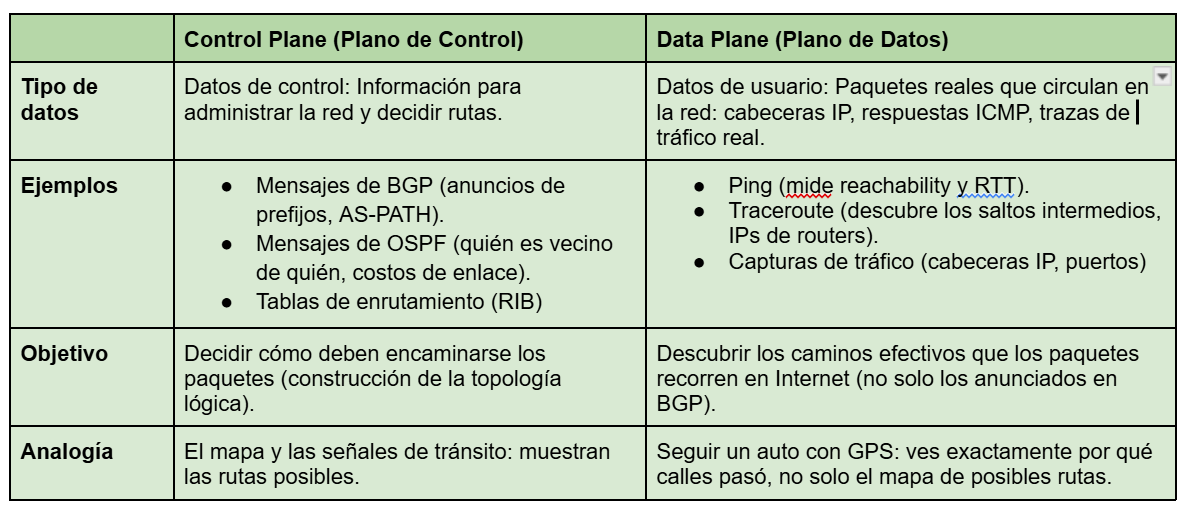
\includegraphics[width=0.9\textwidth]{Anexos/img/01/control_plane_vs_data_plane_tabla.png}
    \caption{Resumen conceptual de diferencias entre mediciones del plano de control y del plano de datos.}
    \label{fig:control_plane_vs_data_plane}
\end{figure}

En términos prácticos, BGP suele ofrecer un acceso escalable a rutas interdominio, mientras que \textit{traceroute} puede revelar enlaces que no aparecen en BGP (por ejemplo, enlaces en la periferia o enlaces que no son parte de la mejor ruta anunciada hacia un prefijo).

\subsection{Fuentes del plano de control: colectores BGP}

Los colectores BGP son infraestructuras públicas de recolección de información BGP diseñadas para observar el enrutamiento interdominio desde múltiples ubicaciones. En general, un colector establece sesiones BGP con distintos Sistemas Autónomos (los \textit{vantage points}) y almacena la información de enrutamiento que recibe.

Dos formas comunes de acceso a datos BGP son:
\begin{itemize}
    \item \textbf{RIBs (\textit{Routing Information Base})}: \textit{snapshots} periódicos de las tablas de enrutamiento observadas por el colector.
    \item \textbf{Updates}: mensajes incrementales que reflejan cambios en rutas (anuncios y retiros) y capturan parte de la dinámica del protocolo.
\end{itemize}

En este trabajo, las RIBs se usan como base para obtener rutas estables y construir la topología a nivel de AS. Los \textit{updates} pueden complementar este proceso cuando se desea observar variaciones temporales o rutas alternativas.

\subsection{Fuentes del plano de datos: medición activa}

Las mediciones del plano de datos, como \textit{traceroute}, permiten observar rutas a nivel de IP y, mediante técnicas de mapeo IP$\rightarrow$ASN, aproximar rutas a nivel de AS. Este tipo de medición presenta desafíos adicionales:
\begin{itemize}
    \item \textbf{Sesgo por puntos de medición}: la cobertura depende del número y ubicación de los \textit{vantage points}.
    \item \textbf{Aliasing y rutas asimétricas}: múltiples IP pueden corresponder a un mismo router y las rutas pueden diferir entre ida y vuelta.
    \item \textbf{Mapeo IP$\rightarrow$ASN}: no siempre es posible asignar cada salto IP a un ASN con certeza.
\end{itemize}

\subsection{Mapeo IP$\rightarrow$ASN}

Cuando se requiere transformar rutas IP a rutas AS, una estrategia común es el \textit{Longest Prefix Match}: a cada IP se le asigna el ASN del prefijo BGP más específico que la contiene, a partir de tablas de prefijos obtenidas de RIBs. Si un salto no puede mapearse (por ejemplo, por ausencia de prefijo o ambigüedad), se marca como desconocido o se omite el tramo según el criterio del análisis.

\subsection{Construcción del grafo a partir de datos BGP}

El objetivo es construir un grafo $G=(V,E)$ donde cada nodo $v \in V$ representa un Sistema Autónomo (ASN) y cada arista $e \in E$ representa adyacencias observadas entre ASes.

\subsubsection{Extracción de adyacencias desde \texttt{AS\_PATH}}

Sea una ruta BGP representada por una secuencia de ASNs:
\[
\texttt{AS\_PATH} = (a_1, a_2, \dots, a_k)
\]
Entonces se agregan adyacencias entre pares consecutivos:
\[
(a_1,a_2), (a_2,a_3), \dots, (a_{k-1},a_k)
\]
Dependiendo de la tarea, estas adyacencias pueden modelarse como aristas no dirigidas (para topología) o dirigidas (cuando se requiere asociar dirección a una relación).

\subsubsection{Limpieza de rutas}

Antes de construir el grafo, es habitual depurar rutas para evitar casos ambiguos o que introducen ruido. Por ejemplo:
\begin{itemize}
    \item descartar rutas con conjuntos de AS (AS-SET) u otras estructuras no lineales,
    \item remover duplicados consecutivos producto de \textit{prepending},
    \item descartar rutas con bucles evidentes,
    \item filtrar ASNs privados si aparecen en los datos.
\end{itemize}

\subsubsection{Ponderación y agregación de aristas}

Cuando una adyacencia aparece en múltiples rutas, se puede llevar un contador de ocurrencias y asociarlo como peso $w(u,v)$, lo que permite:
\begin{itemize}
    \item priorizar enlaces más observados,
    \item filtrar enlaces raros (posibles artefactos) usando umbrales,
    \item comparar estabilidad temporal del grafo entre diferentes fechas.
\end{itemize}

\subsubsection{Limitaciones}

Los grafos derivados de BGP reflejan alcanzabilidad y políticas del plano de control, pero no garantizan representar toda la conectividad física o contractual subyacente. Además, al observarse desde un conjunto limitado de \textit{vantage points}, existen sesgos y enlaces que no serán visibles (por ejemplo, enlaces de peering poco utilizados o rutas alternativas que nunca son seleccionadas como mejor ruta).


	% 2) Marco de inferencia y aprendizaje
	\section{Conceptos adicionales de grafos para modelado} \label{sec:anexo_conceptos_grafos_modelado}

Este anexo fija notación y definiciones básicas sobre grafos utilizadas a lo largo de la tesis, tanto para la construcción de la topología a nivel de Sistemas Autónomos como para el uso de modelos de aprendizaje sobre grafos.

\subsection{Formalización de grafos}

Un grafo es una estructura discreta formada por un conjunto de vértices (o nodos) y un conjunto de aristas que conectan pares de nodos. Formalmente, se define como $G=(V,E)$, donde $V$ es un conjunto no vacío de nodos y $E$ es un conjunto de aristas.

Usamos $v_i \in V$ para denotar que un nodo forma parte del grafo, y $e_{ij}=(v_i,v_j)\in E$ para indicar que existe una arista entre los nodos $v_i$ y $v_j$. En un grafo no dirigido, $e_{ij}$ representa una conexión bidireccional; en un grafo dirigido, la arista tiene orientación y expresa una relación desde $v_i$ hacia $v_j$.

La vecindad de un nodo $v_i$ se define como $N(v_i)=\{v_j \in V : (v_i,v_j)\in E\}$. El número de nodos y aristas se denota por $n=|V|$ y $m=|E|$, respectivamente.

Una representación habitual es la matriz de adyacencia $A\in\mathbb{R}^{n\times n}$, donde:
\[
A_{ij} =
\begin{cases}
1 & \text{si } e_{ij}\in E,\\
0 & \text{si } e_{ij}\notin E.
\end{cases}
\]
En grafos ponderados puede utilizarse $A_{ij}=w_{ij}$ para reflejar el peso asociado a la arista. En problemas de aprendizaje automático suele considerarse, además, una matriz de atributos $X\in\mathbb{R}^{n\times d}$, donde cada fila corresponde a un vector de características de un nodo.

\subsection{Categorías de grafos usadas en modelado}

\begin{itemize}
    \item \textbf{Grafos dirigidos/no dirigidos}: en grafos dirigidos cada arista tiene una dirección específica, indicando un flujo unidireccional entre nodos; en grafos no dirigidos las aristas no tienen orientación y representan conexiones bidireccionales.
    \item \textbf{Grafos ponderados/no ponderados}: en grafos ponderados cada arista posee un valor asociado (por ejemplo, frecuencia de observación, capacidad o costo); en grafos no ponderados solo se modela existencia/ausencia de conexión.
    \item \textbf{Grafos homogéneos/heterogéneos}: en grafos homogéneos nodos y aristas son de un único tipo; en grafos heterogéneos pueden existir distintos tipos de nodos y/o relaciones.
    \item \textbf{Grafos estáticos/dinámicos}: un grafo estático mantiene su topología fija en el tiempo, mientras que un grafo dinámico cambia su estructura (nodos/aristas/pesos) conforme evoluciona el sistema observado.
\end{itemize}

En este trabajo, la topología de conectividad a nivel de AS se modela usualmente como un grafo no dirigido para describir adyacencias, mientras que la inferencia de relaciones económicas requiere distinguir dirección en los enlaces (por ejemplo, proveedor$\rightarrow$cliente).


	\input{Anexos/B_anexo_Inferencia_Relaciones_ASes.tex}
	\section{Fundamentos de Machine Learning} \label{sec:anexo_fundamentos_machine_learning}

Este anexo resume conceptos de aprendizaje automático utilizados en la tesis, con énfasis en (i) el rol de las representaciones vectoriales (\textit{embeddings}) y (ii) el proceso de entrenamiento y evaluación de modelos.

\subsection{Jerarquía conceptual IA, ML y DL}

La Inteligencia Artificial (IA) es un campo de la informática que busca simular el comportamiento de la inteligencia humana, es decir, intenta replicar y automatizar la capacidad del ser humano para tomar decisiones.

Dentro del área de la Inteligencia Artificial, se encuentra el Machine Learning (ML), disciplina que a través del desarrollo de algoritmos y modelos busca que las máquinas aprendan patrones por medio de la experiencia, utilizando datos de entrenamiento y retroalimentación. El objetivo es entrenar un sistema para una tarea específica sin necesidad de programar explícitamente un conjunto de reglas para cada caso.

Finalmente, dentro de ML se encuentra el campo de Deep Learning (DL), un área que se centra en el uso de arquitecturas de redes neuronales profundas para aprender representaciones jerárquicas de los datos de forma automática \cite{deep-learning}.

\begin{figure}[h]
    \centering
    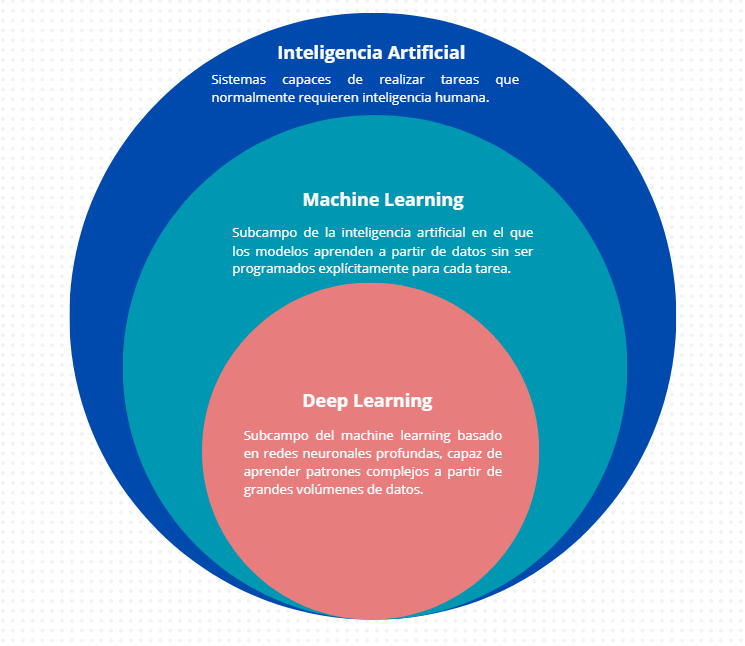
\includegraphics[width=0.75\textwidth]{Anexos/img/03/ia_ml_dl.png}
    \caption{Jerarquía conceptual entre Inteligencia Artificial, Machine Learning y Deep Learning.}
    \label{fig:ia_ml_dl_jerarquia}
\end{figure}

\subsection{Conceptos básicos de aprendizaje automático}

\subsubsection{Tipos de aprendizaje y tareas}

En términos generales, los problemas de aprendizaje se pueden agrupar en:
\begin{itemize}
    \item \textbf{Aprendizaje supervisado}: se cuenta con pares $(x_i,y_i)$, donde $x_i$ representa la entrada (atributos) y $y_i$ la etiqueta objetivo. El modelo aprende una función $f_\theta$ que aproxima $y$ a partir de $x$. Tareas típicas son clasificación y regresión.
    \item \textbf{Aprendizaje no supervisado}: no se dispone de etiquetas; se busca descubrir estructura en los datos (por ejemplo, agrupamiento o reducción de dimensionalidad).
    \item \textbf{Aprendizaje auto-supervisado}: se construyen objetivos a partir de los mismos datos para aprender representaciones útiles sin etiquetas explícitas (por ejemplo, predecir partes faltantes, contexto o transformaciones).
\end{itemize}

En esta tesis, el objetivo principal se relaciona con tareas supervisadas (por ejemplo, clasificación de relaciones económicas entre ASes) y con aprendizaje de representaciones, donde la calidad del \textit{embedding} impacta directamente el desempeño del modelo final.

\subsubsection{Representaciones y \textit{embeddings}}

Una \textbf{representación} corresponde a una codificación de una entidad (por ejemplo, un AS) en una forma que pueda ser procesada por un modelo. En ML, una representación común es un vector numérico $x\in\mathbb{R}^d$ que reúne atributos o descriptores.

Un \textbf{\textit{embedding}} es una representación vectorial densa (de dimensión relativamente baja) que se aprende o construye con el objetivo de preservar información relevante sobre la entidad y su contexto. A diferencia de codificaciones dispersas como \textit{one-hot}, los \textit{embeddings} permiten capturar nociones de similitud: entidades con roles o contextos similares tienden a quedar cercanas en el espacio vectorial.

En el contexto de esta tesis, las representaciones pueden provenir de:
\begin{itemize}
    \item \textbf{Atributos tabulares}: características extraídas desde fuentes como PeeringDB (por ejemplo, tipo de red, políticas, presencia en IXPs).
    \item \textbf{Estructura de conectividad}: representaciones derivadas de rutas BGP o de la topología del grafo, donde el ``contexto'' de un AS está determinado por su vecindad o por sus co-ocurrencias en caminos.
\end{itemize}

\subsubsection{Entrenamiento, validación y evaluación}

En un flujo estándar de aprendizaje supervisado, los datos se separan en conjuntos de \textbf{entrenamiento}, \textbf{validación} y \textbf{prueba}. El entrenamiento ajusta parámetros $\theta$ minimizando una función de pérdida $L(\theta)$ (por ejemplo, entropía cruzada para clasificación), típicamente mediante variantes de descenso por gradiente (por ejemplo, SGD o Adam).

El conjunto de validación se utiliza para seleccionar hiperparámetros (dimensión del \textit{embedding}, tasa de aprendizaje, número de épocas, regularización, etc.) y controlar \textit{overfitting} mediante estrategias como \textbf{early stopping}. El conjunto de prueba se reserva para reportar desempeño final.

En problemas con \textbf{desbalance de clases}, es importante complementar métricas globales (por ejemplo, \textit{accuracy}) con métricas por clase o promediadas (por ejemplo, \textit{precision}, \textit{recall} y $F_1$), y considerar técnicas como ponderación de la pérdida o muestreo estratificado para evitar modelos sesgados hacia la clase mayoritaria.

\subsection{Arquitecturas neuronales clásicas (FFNN, RNN, CNN)}

\subsubsection{Redes Neuronales Feed Forward (FFNN)}

También conocidas como \textit{multilayer perceptrons}, estas arquitecturas representan la forma más simple y fundamental de una red neuronal, sirviendo como base de múltiples modelos de Deep Learning. En esta arquitectura la información fluye exclusivamente hacia ``adelante'', sin bucles o conexiones recurrentes.

El flujo comienza en la capa de entrada, seguida de capas ocultas (típicamente \textit{fully connected}), donde cada neurona se conecta con las neuronas de la capa anterior. El objetivo general es aproximar una función $f(x)$; por ejemplo, en regresión se busca modelar una relación $y=f(x)$.

\subsubsection{Redes Neuronales Recurrentes (RNN)}

Las redes neuronales recurrentes (RNN) son una variante de redes \textit{feed forward} con capacidad de incorporar información previa, es decir, poseen ``memoria''. A diferencia de las FFNN, las RNN introducen conexiones desde estados anteriores hacia el estado actual, lo que permite modelar dependencias temporales.

Esta característica hace a las RNN adecuadas para trabajar con datos secuenciales, como procesamiento de lenguaje natural y predicción de series temporales.

\subsubsection{Redes Neuronales Convolucionales (CNN)}

Las redes neuronales convolucionales (CNN) son un tipo especializado de modelo diseñado para procesar datos con estructura de grilla (por ejemplo, imágenes). Estas redes aplican operaciones de convolución mediante filtros (kernels) que aprenden patrones locales (bordes, texturas, formas), combinándolos jerárquicamente a través de múltiples capas.

Estas arquitecturas ilustran por qué, para datos relacionales de tipo grafo, es necesario incorporar explícitamente la estructura de conectividad; esto motiva el uso de Redes Neuronales de Grafos (GNNs), descritas en el anexo siguiente.


	\section{Redes Neuronales de Grafos (GNNs)} \label{sec:anexo_gnns}

Las Redes Neuronales de Grafos (GNNs, \textit{Graph Neural Networks}) son una familia de modelos de aprendizaje profundo diseñada para realizar predicciones a partir de datos representados como grafos. A diferencia de redes neuronales convencionales (por ejemplo, FFNN o CNN), que asumen estructuras euclidianas (vectores o grillas), las GNNs combinan explícitamente atributos de nodos/aristas con la conectividad del grafo \cite{gnnReviewMethods}.

\subsection{Niveles de aprendizaje sobre grafos}

Dependiendo de la tarea, una GNN puede entrenarse para producir salidas a distintos niveles:
\begin{itemize}
    \item \textbf{Nivel de nodo}: clasificación o regresión por nodo, utilizando tanto sus atributos como la información de su vecindad.
    \item \textbf{Nivel de arista}: clasificación o predicción de enlaces (por ejemplo, inferir si existe una relación entre dos nodos y de qué tipo).
    \item \textbf{Nivel de grafo}: clasificación o regresión de grafos completos, aprendiendo una representación global del grafo.
\end{itemize}

\subsection{Motivación y propiedades}

El uso de GNNs se justifica por propiedades propias de los grafos:
\begin{itemize}
    \item \textbf{Relaciones explícitas}: las aristas codifican dependencias, jerarquías o interacciones que un modelo sobre vectores no captura directamente.
    \item \textbf{Tamaño variable}: los grafos pueden tener distinto número de nodos/aristas, sin requerir \textit{padding} a un tamaño fijo.
    \item \textbf{Invarianza a permutaciones}: el modelo debe producir representaciones consistentes ante re-etiquetados de nodos (isomorfismos), evitando depender del orden de la matriz de adyacencia.
    \item \textbf{Estructura no euclidiana}: la noción de ``cercanía'' no se reduce a distancias en una grilla; la conectividad y vecindad definen el contexto relevante.
\end{itemize}

\subsection{Idea general: propagación de mensajes (\textit{message passing})}

La base de muchas GNNs modernas es la \textbf{propagación de mensajes}, donde en cada capa $l$ se actualiza la representación de cada nodo agregando información desde su vecindad. Sea $\mathbf{h}_i^{(l)}$ el \textit{embedding} del nodo $i$ en la capa $l$ y $\mathcal{N}(i)$ su conjunto de vecinos. Una formulación general consiste en:
\[
\mathbf{m}_i^{(l)}=\mathrm{AGG}^{(l)}\Big(\big\{\phi^{(l)}(\mathbf{h}_i^{(l)},\mathbf{h}_j^{(l)},\mathbf{e}_{ij}) : j\in\mathcal{N}(i)\big\}\Big),
\]
\[
\mathbf{h}_i^{(l+1)}=\psi^{(l)}(\mathbf{h}_i^{(l)},\mathbf{m}_i^{(l)}),
\]
donde $\phi^{(l)}$ define el mensaje, $\mathrm{AGG}^{(l)}$ es una función de agregación (por ejemplo, suma/promedio/máximo) y $\psi^{(l)}$ es la función de actualización (típicamente una transformación lineal seguida de una no linealidad).

Para tareas a nivel de grafo, se utiliza además una operación de \textit{readout} que agrega representaciones de nodos en una representación global (por ejemplo, suma o promedio sobre todos los nodos).

\subsection{Message Passing Neural Networks (MPNN)}

Las \textit{Message Passing Neural Networks} (MPNN) proponen un marco unificado para arquitecturas basadas en propagación de mensajes, separando una fase de agregación local y una fase de lectura global cuando corresponde \cite{mpnn}. Este marco resulta útil para entender GCN y GAT como casos particulares de la misma idea: combinar información de vecinos para refinar representaciones nodo a nodo.

\subsection{Graph Convolutional Networks (GCN)}

Las \textit{Graph Convolutional Networks} (GCN) implementan un esquema de agregación por promedio normalizado de vecinos. Una formulación ampliamente utilizada es \cite{GCN-formula}:
\[
H^{(l+1)}=\sigma\left(\tilde{D}^{-\frac{1}{2}}\tilde{A}\tilde{D}^{-\frac{1}{2}}H^{(l)}W^{(l)}\right),
\]
donde $H^{(l)}\in\mathbb{R}^{n\times d_l}$ es la matriz de representaciones de nodos en la capa $l$, $W^{(l)}$ es una matriz de pesos entrenables, $\sigma$ es una función de activación, $\tilde{A}=A+I$ agrega auto-conexiones, y $\tilde{D}$ es la matriz diagonal con $\tilde{D}_{ii}=\sum_j \tilde{A}_{ij}$.

\subsection{Graph Attention Networks (GAT)}

Las \textit{Graph Attention Networks} (GAT) incorporan un mecanismo de atención para ponderar de forma diferenciada la contribución de cada vecino al actualizar un nodo \cite{GAT}. Una formulación típica por capa es:
\[
\mathbf{z}_i^{(l)}=W^{(l)}\mathbf{h}_i^{(l)},
\]
\[
e_{ij}^{(l)}=\mathrm{LeakyReLU}\left(\mathbf{a}^{(l)\top}[\mathbf{z}_i^{(l)} \Vert \mathbf{z}_j^{(l)}]\right),
\]
\[
\alpha_{ij}^{(l)}=\frac{\exp(e_{ij}^{(l)})}{\sum_{k\in\mathcal{N}(i)}\exp(e_{ik}^{(l)})},
\]
\[
\mathbf{h}_i^{(l+1)}=\sigma\left(\sum_{j\in\mathcal{N}(i)}\alpha_{ij}^{(l)}\mathbf{z}_j^{(l)}\right),
\]
donde $\Vert$ denota concatenación, $\mathbf{a}^{(l)}$ es un vector de parámetros entrenables y $\alpha_{ij}^{(l)}$ representa el peso de atención asociado a la arista $(i,j)$. En la práctica se utilizan variantes como \textit{multi-head attention} para estabilizar y enriquecer la agregación.

\subsection{Consideraciones prácticas en grafos grandes}

En grafos de gran escala, el costo de agregar sobre todos los vecinos puede ser alto. Por ello, muchas implementaciones incorporan \textbf{muestreo de vecindad} y entrenamiento por mini-batches, lo cual permite aproximar la agregación manteniendo escalabilidad. Modelos como GraphSAGE formalizan esta idea mediante muestreo y agregación inductiva \cite{GraphSAGE}.



	% 3) Datos, analisis y configuracion experimental
	\section{Análisis exploratorio y características del dataset} \label{sec:anexo_analisis_exploratorio_caracteristicas_dataset}

\subsection{Exploración de datos de PeeringDB}  \label{sec:anexo_exploracion_datos_peeringdb}





A continuación, se presenta una breve exploración del archivo de peeringDB correspondiente a la fecha de 02/01/2024 
\texttt{peeringdb\_2\_dump\_2024\_02\_01.json}, el cual contiene información pública utilizada para describir la infraestructura de Sistemas Autónomos (ASes), Internet Exchange Points (IXPs) y organizaciones asociadas. \\


El archivo se encuentra en formato \texttt{JSON} y contiene las siguientes claves principales:
\begin{verbatim}
dict_keys(['ixlan', 'ixfac', 'carrierfac', 'netixlan', 'ix', 'net', 
           'netfac', 'poc', 'api', 'fac', 'carrier', 'org', 
           'ixpfx', 'as_set', 'campus'])
\end{verbatim}

Las tablas más importantes para este estudio son las siguientes :
\begin{itemize}
    \item \textbf{net}: Las redes (AS) registradas en PeeringDB, junto con su información  de país, tipo de organización, tráfico e información de peering.
    
    \item \textbf{ix}: Información general de los Internet Exchange Points (IXPs) con su información de nombre, país, ciudad, organización administradora, etc.

    \item \textbf{fac}: Representa las instalaciones o centros de datos donde las redes y los IXPs están físicamente presentes. Incluye información geográfica y de estado operativo.
    
    \item \textbf{netfac}: Relaciona cada red (\textbf{net}) con los centros de datos (\textbf{fac}) en los que tiene presencia.

    \item \textbf{org}: Contiene información sobre las organizaciones administradoras de redes, IXPs y facilities, como su nombre, país y tipo de entidad.

\end{itemize}


\subsubsection*{Exploración de la tabla \texttt{net}}

Esta tabla recopila la información disponible en PeeringDB sobre diferentes Sistemas Autónomos presentes en Internet y que se tiene su registro en dicha plataforma. Cada elemento representa un AS y describe atributos como tipo de organización, tráfico, políticas de peering, características de conectividad entre otras. 
Al transformar esta a un Data Frame, esta contiene \textbf{29,418} filas correspondiente a información sobre diferentes ASes y \textbf{40} columnas correspondiente a atributos de estos.\\

En primer lugar, se analizaron las columnas y sus tipos de datos, identificando \textbf{6 columnas numéricas}, \textbf{27 categóricas} y \textbf{6 booleanas}.


\begin{lstlisting}[language=Python, caption={Columnas del conjunto de datos \texttt{net}.}, label={lst:columnas_net}]
=== Columnas numéricas ===
['fac_count', 'id', 'ix_count', 'org_id', 'info_prefixes6', 'info_prefixes4']

=== Columnas categóricas ===
['status', 'looking_glass', 'route_server', 'netixlan_updated', 'info_ratio', 
 'status_dashboard', 'rir_status', 'created', 'name_long', 'policy_general', 
 'website', 'updated', 'info_types', 'rir_status_updated', 'netfac_updated', 
 'info_traffic', 'policy_locations', 'name', 'info_scope', 'notes', 'policy_url', 
 'poc_updated', 'info_type', 'social_media', 'policy_contracts', 'aka', 'irr_as_set']

=== Columnas booleanas ===
['policy_ratio', 'info_unicast', 'allow_ixp_update', 'info_multicast', 
 'info_never_via_route_servers', 'info_ipv6']
\end{lstlisting}


Tras esta primera exploración, se decidió conservar las columnas categóricas relevantes para el estudio, principalmente aquellas que entregan información sobre políticas de conexión, tráfico y alcance de red. Las categorías identificadas se resumen en la Tabla~\ref{tab:categorias_peeringdb_clara}.




\begin{table}[H]
\centering
\caption{Resumen de las categorías presentes en las columnas categóricas seleccionadas del conjunto \texttt{net} de PeeringDB.}
\label{tab:categorias_peeringdb_clara}
\begin{tabularx}{\textwidth}{lX}
\hline
\textbf{Columna} & \textbf{Categorías y ejemplos de valores} \\
\hline

\texttt{policy\_contracts} (4 categorías) &
Required, Not Required, Private Only, (vacío). \\

\texttt{info\_type} (10 categorías) &
NSP, Content, Non-Profit, Cable/DSL/ISP, Educational/Research, 
Network Services, Enterprise, Route Server, Route Collector, (vacío). \\

\texttt{info\_scope} (11 categorías) &
Global, Europe, North America, Regional, Asia Pacific, South America, 
Not Disclosed, Australia, Middle East, Africa, (vacío). \\

\texttt{policy\_locations} (6 categorías) &
Required – International, Not Required, Preferred, Required – US, Required – EU, (vacío). \\

\texttt{info\_traffic} (19 categorías) &
0–20 Mbps, 20–100 Mbps, 5–10 Gbps, 10–20 Gbps, 100–200 Gbps, 500–1000 Gbps, 
1–5 Tbps, 50–100 Tbps, 100+ Tbps, (vacío). \\

\texttt{info\_types} (9 categorías) &
NSP, Content, Non-Profit, Cable/DSL/ISP, Educational/Research, 
Network Services, Enterprise, Route Server, Route Collector. \\

\texttt{policy\_general} (5 categorías) &
Restrictive, Open, Selective, No, (vacío). \\

\texttt{info\_ratio} (7 categorías) &
Balanced, Heavy Inbound, Heavy Outbound, Mostly Inbound, 
Mostly Outbound, Not Disclosed, (vacío). \\

\hline
\end{tabularx}
\end{table}



Posteriormente, se analizó los valores faltantes en las distintas columnas.  
En el caso de las columnas numéricas, se consideraron faltantes los valores \texttt{NaN} y aquellos igual a cero (Tabla~\ref{tab:faltantes_numericos}).


\begin{table}[H]
\centering
\caption{Porcentaje de valores faltantes o nulos en columnas numéricas del conjunto \texttt{net}.}
\label{tab:faltantes_numericos}
\begin{tabular}{lcc}
\hline
\textbf{Columna} & \textbf{Faltantes} & \textbf{\% Faltantes} \\
\hline
\texttt{fac\_count}       & 17,617 & 59.89 \\
\texttt{ix\_count}        & 14,077 & 47.85 \\
\texttt{info\_prefixes6}  & 11,870 & 40.35 \\
\texttt{info\_prefixes4}  & 9,107  & 30.96 \\
\texttt{id}               & 0      & 0.00 \\
\texttt{org\_id}          & 0      & 0.00 \\
\hline
\end{tabular}
\end{table}

De igual forma para las columnas categóricas s consideraron como faltantes los valores \texttt{NaN} y los string vacios. Los resultados se muestran en la Tabla~\ref{tab:faltantes_categoricas}.

\begin{table}[H]
\centering
\caption{Porcentaje de valores faltantes en las columnas categóricas seleccionadas del conjunto \texttt{net} de PeeringDB.}
\label{tab:faltantes_categoricas}
\renewcommand{\arraystretch}{1.2}
\begin{tabular}{lcc}
\hline
\textbf{Columna} & \textbf{Faltantes} & \textbf{\% Faltantes} \\
\hline
\texttt{info\_traffic}      & 12,047 & 40.95 \\
\texttt{info\_type}         & 8,439  & 28.69 \\
\texttt{policy\_contracts}  & 1,462  & 4.97  \\
\texttt{policy\_general}    & 1,352  & 4.60  \\
\texttt{policy\_locations}  & 1,353  & 4.60  \\
\texttt{info\_ratio}        & 663    & 2.25  \\
\texttt{info\_scope}        & 370    & 1.26  \\
\texttt{info\_types}        & 0      & 0.00  \\
\hline
\end{tabular}
\end{table}


Finalmente, la Tabla~\ref{tab:categorias_categoricas} resume las columnas categóricas seleccionadas junto con el número de categorías únicas y algunos ejemplos representativos.  
Este resumen permite identificar de forma clara la diversidad de información contenida en PeeringDB y la relevancia de cada atributo para su posterior uso en la construcción de modelos basados en grafos.


\begin{table}[H]
\centering
\caption{Resumen de columnas categóricas y número de categorías únicas en PeeringDB.}
\label{tab:categorias_categoricas}
\begin{tabular}{lcc}
\hline
\textbf{Columna} & \textbf{Categorías únicas} & \textbf{Ejemplos de categorías} \\
\hline
policy\_general & 5 & Open, Selective, Restrictive, No \\
info\_type & 10 & NSP, Content, Non-Profit, Enterprise, Route Server \\
info\_scope & 11 & Global, Europe, North America, Regional, Asia Pacific \\
policy\_locations & 6 & Required - US, Required - EU, Not Required \\
info\_traffic & 18 & 1-5Gbps, 100-200Gbps, 10-20Tbps, 0-20Mbps \\
info\_ratio & 7 & Balanced, Heavy Inbound, Mostly Outbound \\
\hline
\end{tabular}
\end{table}





A continuación, algunas figuras para entender los datos.\\





\begin{figure}[H]
    \centering
    % === 1ra fila ===
    \begin{subfigure}[b]{0.48\textwidth}
        \centering
        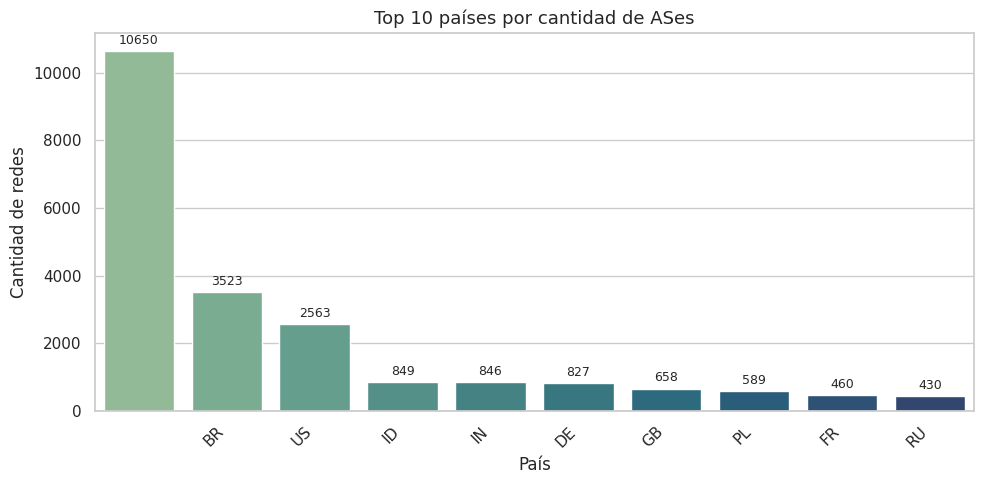
\includegraphics[width=\textwidth]{img/anexoPeeringDB/Top_10_países_por_cantidad_de_ASes.png}
        \caption{Top 10 países con mayor cantidad de ASes registrados en PeeringDB.}
        \label{fig:Top_10_países_por_cantidad_de_ASes}
    \end{subfigure}
    \hfill
    \begin{subfigure}[b]{0.48\textwidth}
        \centering
        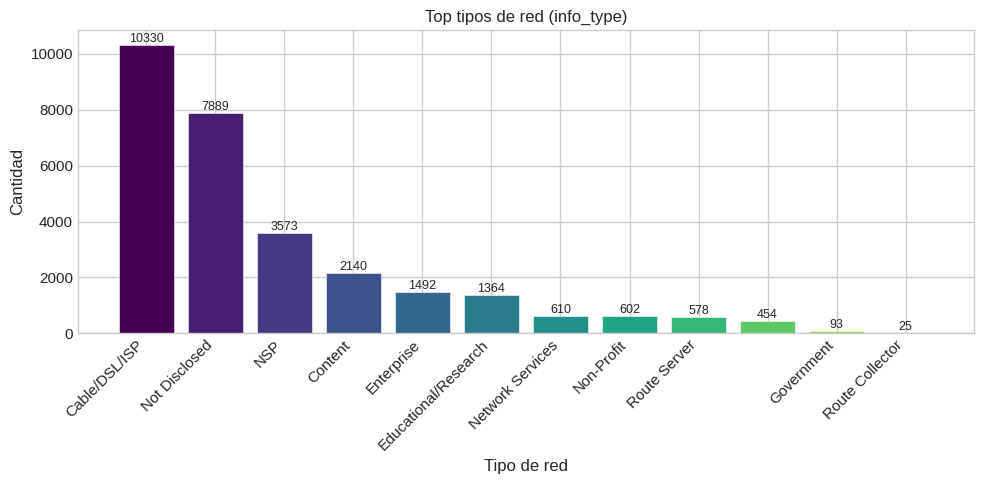
\includegraphics[width=\textwidth]{img/anexoPeeringDB/Top_tipos_de_red_info_type.png}
        \caption{Top tipos de red (\texttt{info\_type}) en ASes registrados en PeeringDB.}
        \label{fig:Top_tipos_de_red_info_type}
    \end{subfigure}

    % === 2da fila ===
    \vspace{5mm}
    \begin{subfigure}[b]{0.48\textwidth}
        \centering
        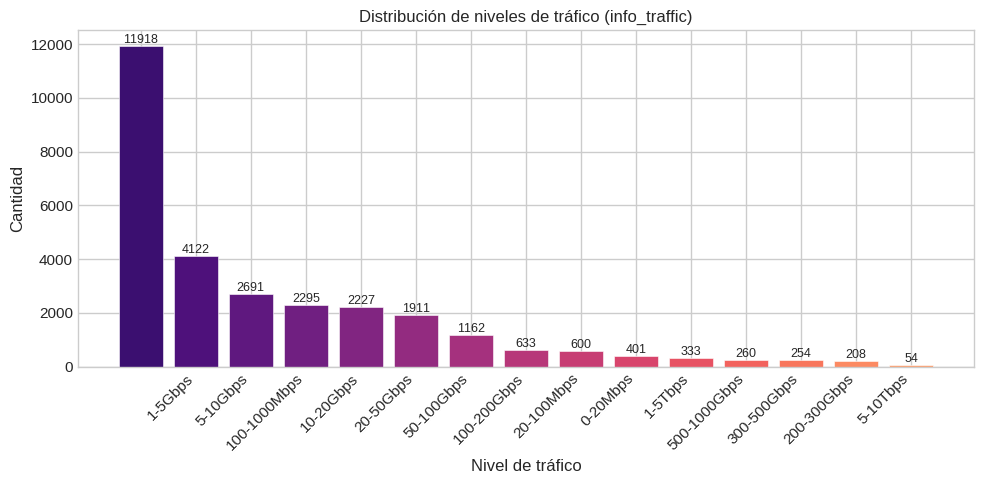
\includegraphics[width=\textwidth]{img/anexoPeeringDB/Distribución_de_niveles_de_tráfico_info_traffic.png}
        \caption{Distribución de niveles de tráfico (\texttt{info\_traffic}).}
        \label{fig:Distribución_de_niveles_de_tráfico_info_traffic}
    \end{subfigure}
    \hfill
    \begin{subfigure}[b]{0.48\textwidth}
        \centering
        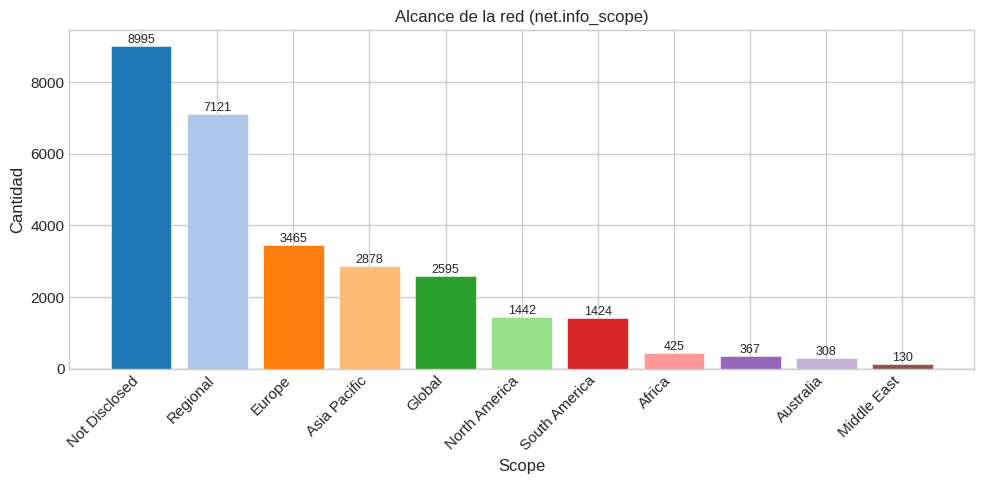
\includegraphics[width=\textwidth]{img/anexoPeeringDB/Alcance_de_la_red_info_scope.png}
        \caption{Alcance de la red (\texttt{info\_scope}).}
        \label{fig:Alcance_de_la_red_info_scope}
    \end{subfigure}

    % === 3ra fila ===
    \vspace{5mm}
    \begin{subfigure}[b]{0.48\textwidth}
        \centering
        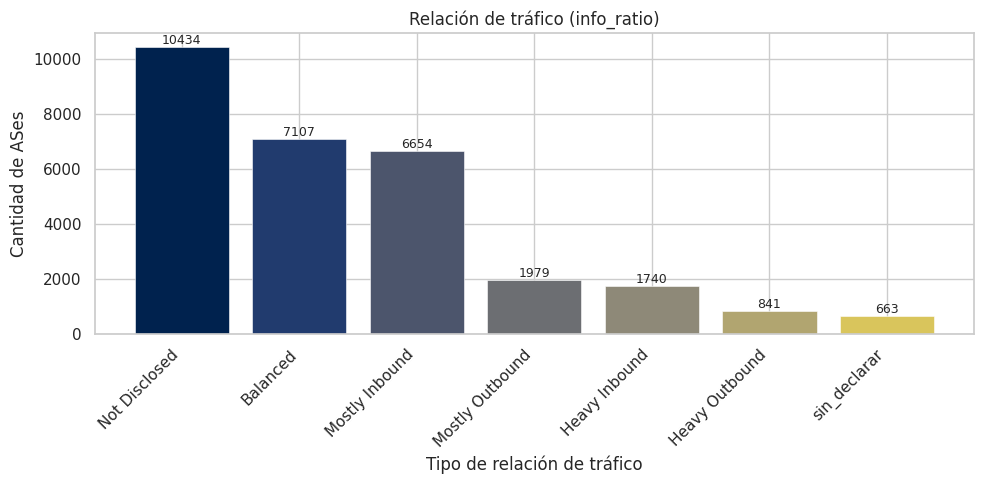
\includegraphics[width=\textwidth]{img/anexoPeeringDB/Relación_de_traficoinfo_ratio.png}
        \caption{Relación de tráfico (\texttt{info\_ratio}).}
        \label{fig:Relación_de_traficoinfo_ratio}
    \end{subfigure}
    \hfill
    \begin{subfigure}[b]{0.48\textwidth}
        \centering
        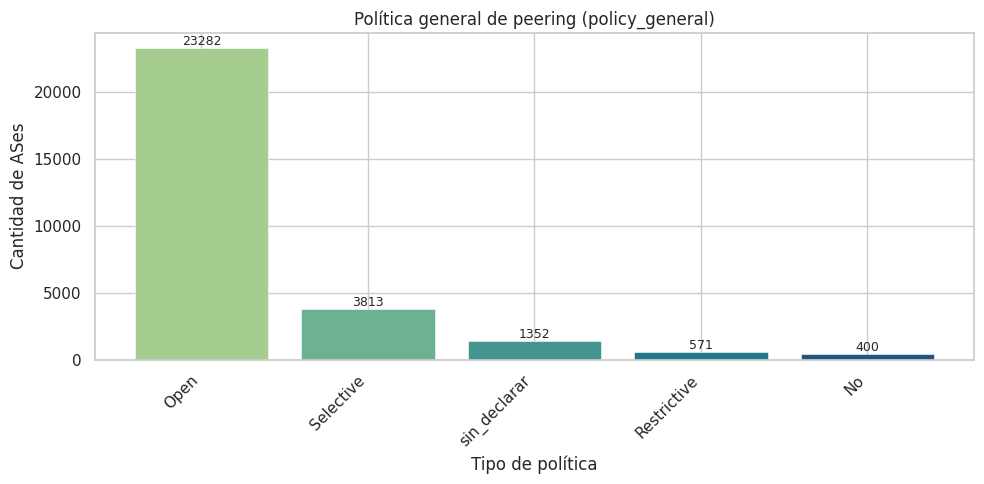
\includegraphics[width=\textwidth]{img/anexoPeeringDB/Politica_general_de_peering_policy_general.png}
        \caption{Política general de peering (\texttt{policy\_general}).}
        \label{fig:Politica_general_de_peering_policy_general}
    \end{subfigure}

    % === 4ta fila ===
    \vspace{5mm}
    \begin{subfigure}[b]{0.48\textwidth}
        \centering
        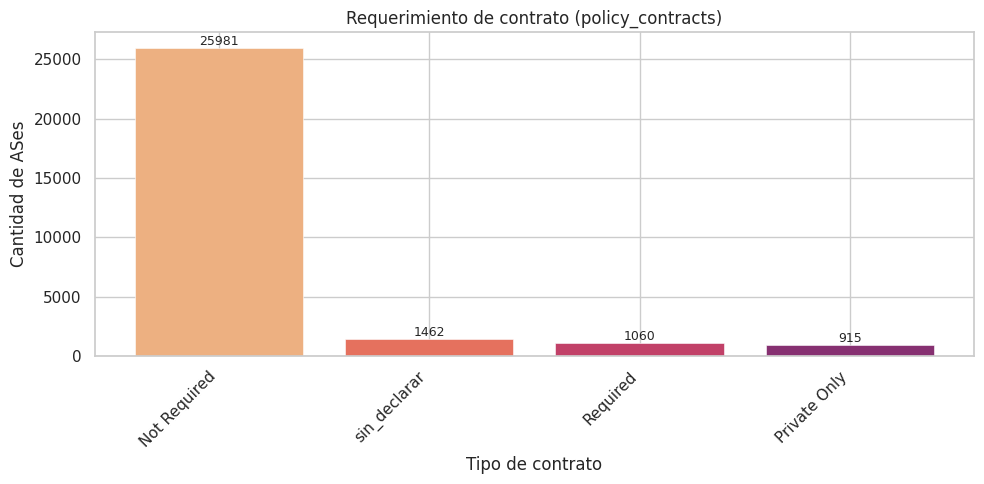
\includegraphics[width=\textwidth]{img/anexoPeeringDB/Requerimiento_de_contrato_policy_contracts.png}
        \caption{Requerimiento de contrato (\texttt{policy\_contracts}).}
        \label{fig:Requerimiento_de_contrato_policy_contracts}
    \end{subfigure}
    \hfill
    \begin{subfigure}[b]{0.48\textwidth}
        \centering
        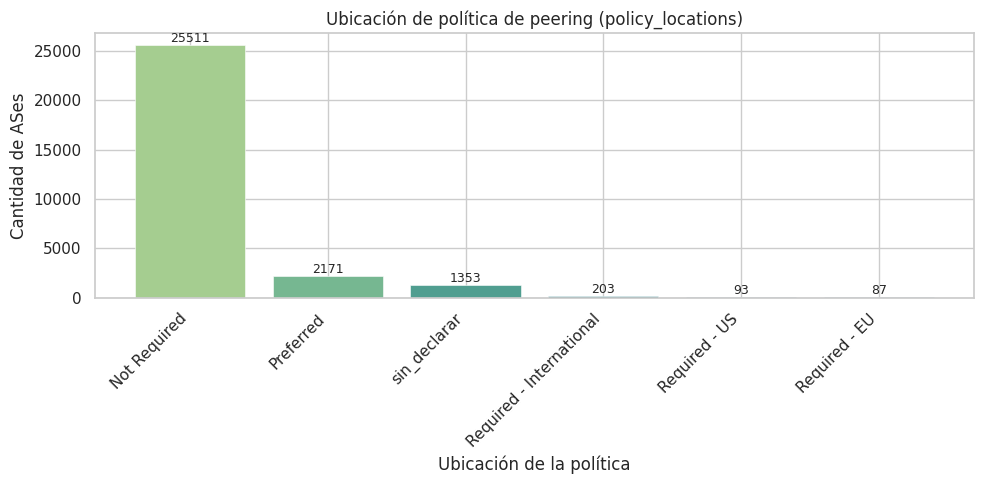
\includegraphics[width=\textwidth]{img/anexoPeeringDB/Ubicacion_de_política_de_peering_policy_locations.png}
        \caption{Ubicación de política de peering (\texttt{policy\_locations}).}
        \label{fig:Ubicacion_de_política_de_peering_policy_locations}
    \end{subfigure}


    \caption{Visualización general de las principales variables categóricas y numéricas del conjunto \texttt{net} de PeeringDB.}
    \label{fig:graficos_peeringdb_completo}
\end{figure}







\begin{figure}[H]
    \centering
    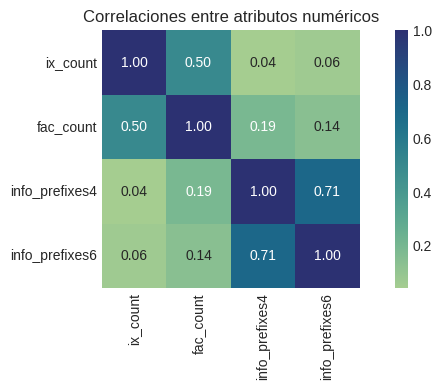
\includegraphics[width=0.6\textwidth]{img/anexoPeeringDB/Correlaciones_entre_atributos_numericos.png}
    \caption{Matriz de correlación entre los atributos numéricos extraidos de PeeringDB.}
    \label{fig:Correlaciones_entre_atributos_numericos}
\end{figure}

Con la visualización de la Figura~\ref{fig:Correlaciones_entre_atributos_numericos} podemos decir:
\begin{itemize}
    \item los AS que anuncian muchos prefijos IPv4 tienden también a anunciar muchos prefijos IPv6. Puedes esperar colinealidad entre ambos.
    \item más IXPs suele venir acompañado de presencia en más facilities (tamaño/cobertura del AS).
\end{itemize}



\begin{table}[H]
\centering
\caption{Porcentaje de filas sin información por columna (antes de limpieza).}
\label{tab:faltantes_net}
\begin{tabular}{l l r r}
\toprule
\textbf{columna} & \textbf{tipo} & \textbf{sin\_info} & \textbf{porcentaje \%} \\
\midrule
info\_traffic      & categórica & 12047 & 40.95 \\
info\_type         & categórica & 8439  & 28.69 \\
policy\_contracts  & categórica & 1462  & 4.97  \\
policy\_general    & categórica & 1352  & 4.60  \\
policy\_locations  & categórica & 1353  & 4.60  \\
info\_ratio        & categórica & 663   & 2.25  \\
info\_scope        & categórica & 370   & 1.26  \\
info\_prefixes4    & numérica   & 0     & 0.00  \\
fac\_count         & numérica   & 0     & 0.00  \\
ix\_count          & numérica   & 0     & 0.00  \\
info\_prefixes6    & numérica   & 0     & 0.00  \\
\bottomrule
\end{tabular}
\end{table}



\subsection{Atributos numéricos}
\label{subsec:attr_num_peeringdb}

La Figura~\ref{fig:attr_num_peeringdb} muestra la distribución de cuatro atributos numéricos provenientes de PeeringDB, tras aplicar el preprocesamiento definido (transformación logarítmica y normalización min--max a $[0,1]$). Para cada atributo se incluye además la media (línea roja) y la mediana (línea azul), con el fin de evidenciar asimetrías y posibles valores extremos.

\begin{figure}[H]
    \centering
    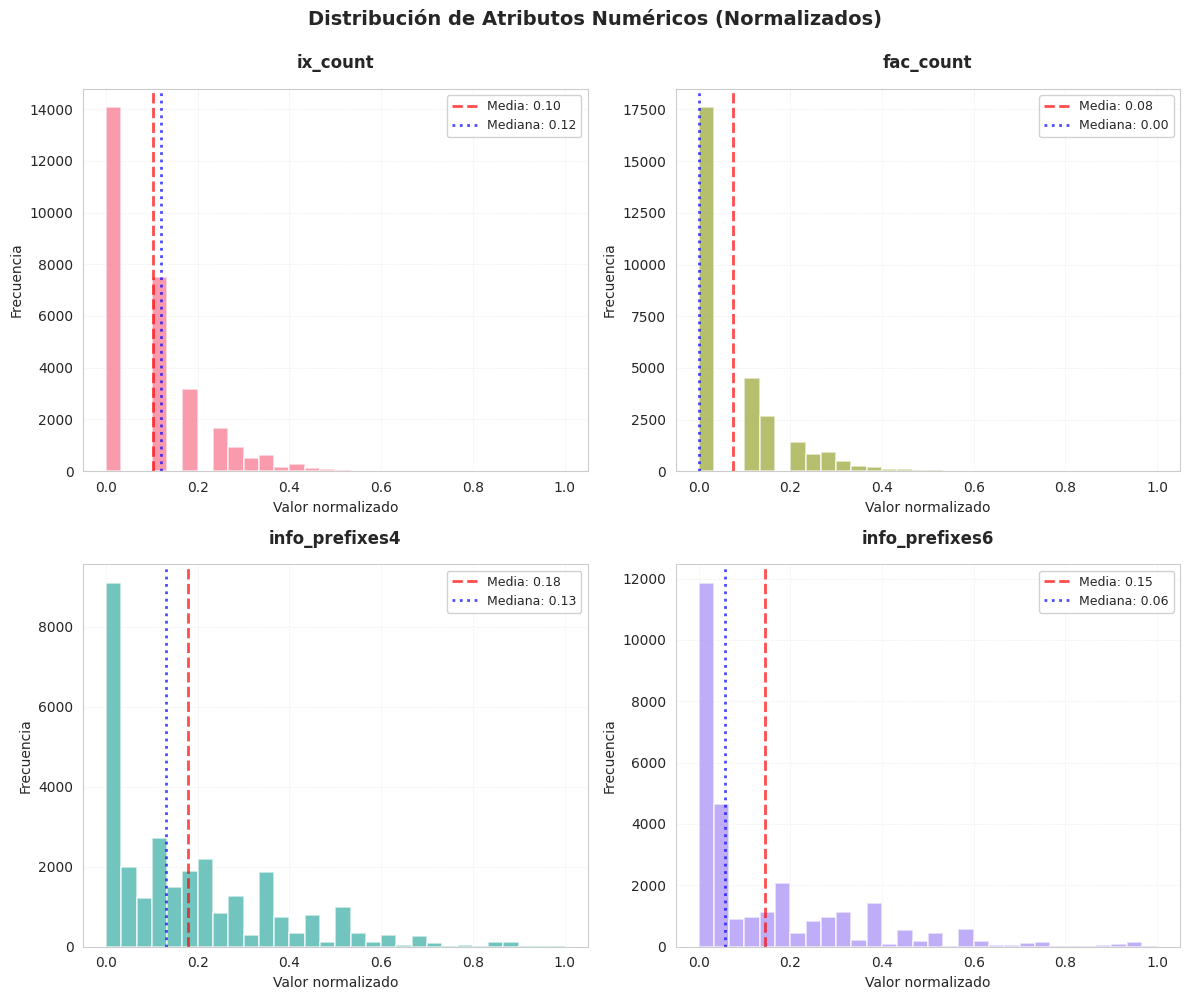
\includegraphics[width=0.85\linewidth]{Anexos/attr_num_peeringdb.png}
    \caption{Distribución de atributos numéricos de PeeringDB normalizados ($[0,1]$). Se muestran \texttt{ix\_count}, \texttt{fac\_count}, \texttt{info\_prefixes4} e \texttt{info\_prefixes6}, junto con la media (rojo) y la mediana (azul).}
    \label{fig:attr_num_peeringdb}
\end{figure}

\paragraph{Media vs.\ mediana: sesgo y presencia de outliers.}
En general, la media se ubica a la derecha de la mediana (media $>$ mediana), lo cual es consistente con distribuciones con \emph{cola derecha}. Esto sugiere la presencia de pocos AS con valores muy altos (outliers) que elevan la media, mientras que la mayoría de los AS se concentra en valores bajos.

\paragraph{Comparación entre atributos.}
\begin{itemize}
    \item \textbf{\texttt{ix\_count}:} la mayoría de los AS participa en pocos IXPs, y existe un grupo reducido con participación en muchos IXPs.
    \item \textbf{\texttt{fac\_count}:} la distribución está fuertemente concentrada cerca de 0; muchos AS reportan pocas (o ninguna) facilities, y pocos AS acumulan un número alto.
    \item \textbf{\texttt{info\_prefixes4} y \texttt{info\_prefixes6}:} muestran mayor variabilidad y una cola larga; un conjunto pequeño de AS anuncia muchos prefijos, mientras que la mayoría anuncia pocos.
\end{itemize}

\paragraph{Efecto del preprocesamiento (log + min--max).}
Aunque los atributos fueron normalizados a $[0,1]$, las distribuciones permanecen ``pegadas'' a 0. Esto indica que, incluso tras la transformación logarítmica, la mayoría de los AS mantiene valores pequeños en comparación con el máximo observado. Este comportamiento es típico en redes reales, donde coexisten pocos AS muy grandes (p.\,ej., backbone/tier-1 o redes altamente conectadas) y una gran cantidad de AS pequeños.

\paragraph{Implicancias para el modelado.}
Estas distribuciones sugieren que:
\begin{itemize}
    \item existen \textbf{outliers potencialmente relevantes} (AS muy grandes),
    \item la \textbf{mediana} describe mejor al AS ``típico'' que la media,
    \item podría ser útil evaluar alternativas robustas si el modelo es sensible a extremos (p.\,ej., \emph{RobustScaler}, winsorización o clipping por percentiles).
\end{itemize}




\subsubsection{Atributos categóricos}
\label{subsec:attr_cat_peeringdb}

La Figura~\ref{fig:attr_cat_peeringdb} muestra la distribución de atributos categóricos extraídos desde PeeringDB. En general, se observa un marcado \textbf{desbalance de clases} en la mayoría de variables, con categorías dominantes (muy frecuentes) y un conjunto de categorías raras con baja representación. Este patrón es relevante porque impacta directamente en la representación mediante \emph{one-hot encoding} (alta esparsidad) y en la contribución efectiva de cada atributo al modelo.

\begin{figure}[H]
    \centering
    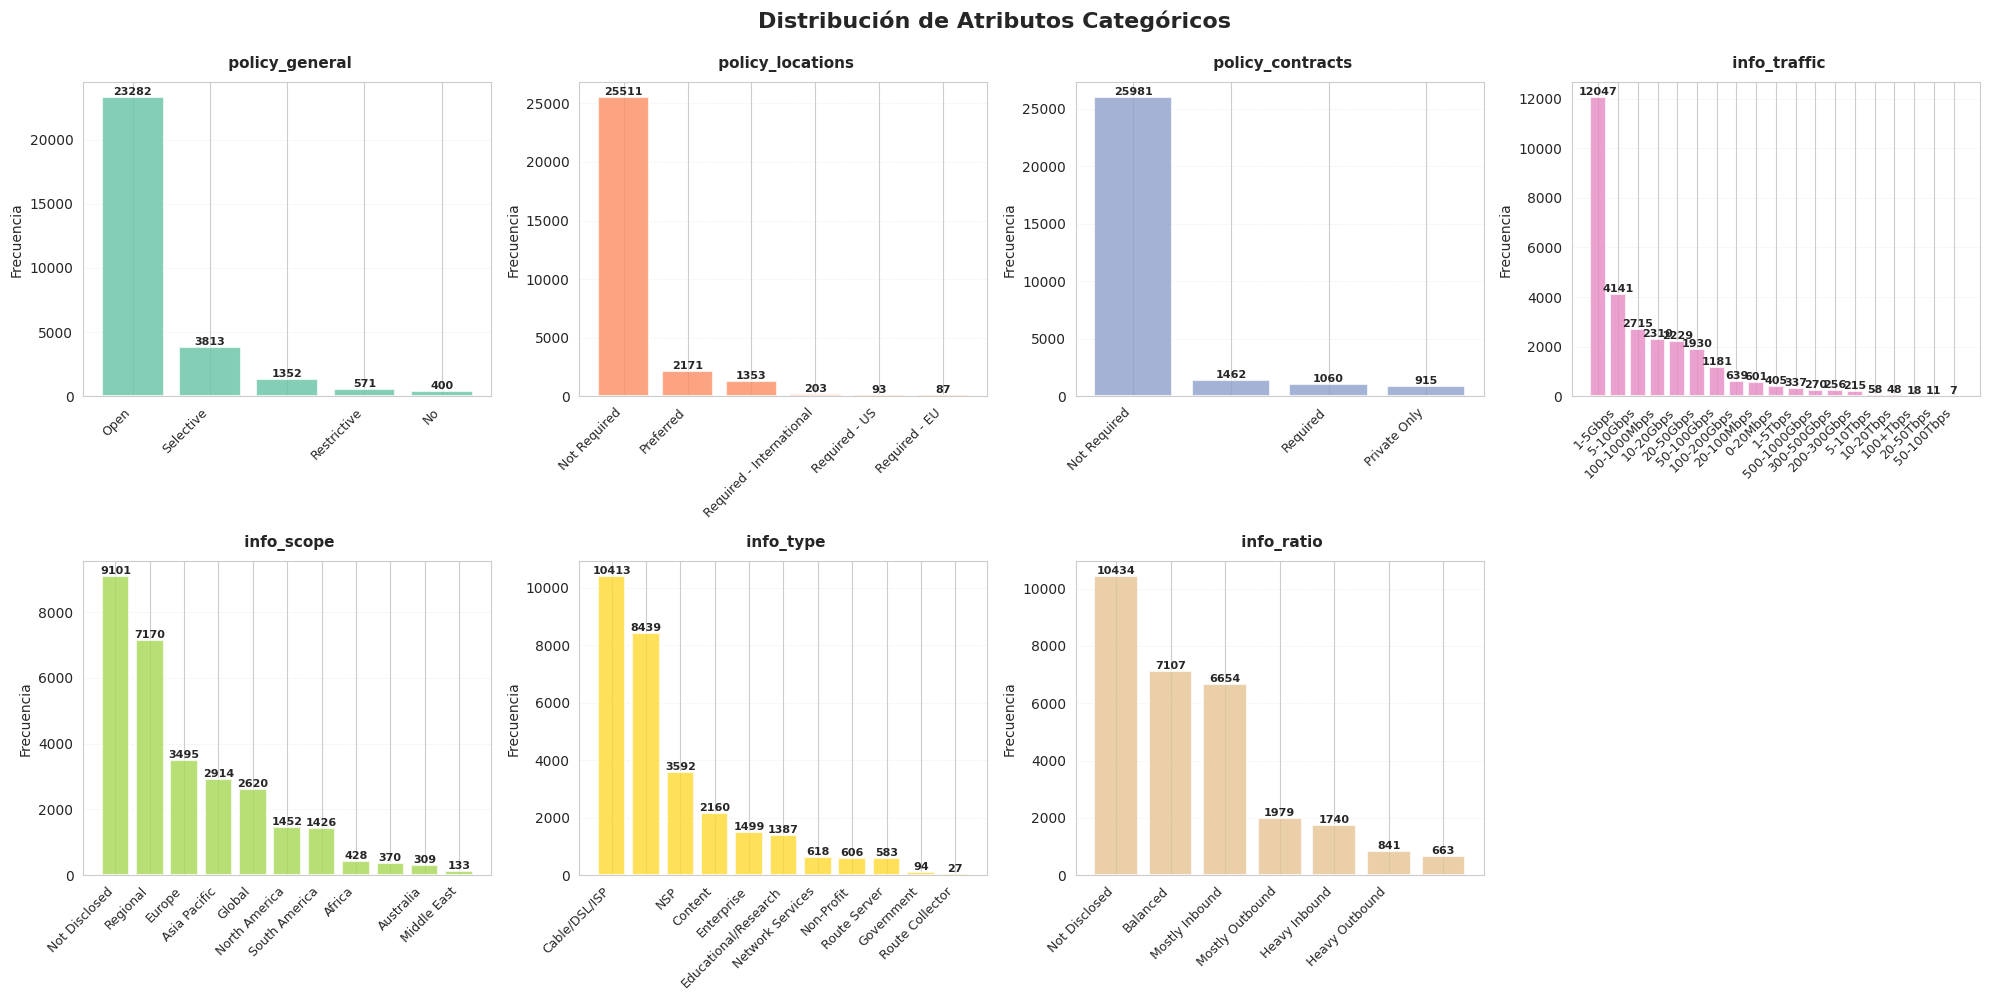
\includegraphics[width=0.95\linewidth]{Anexos/attr_cat_peeringdb.png}
    \caption{Distribución de atributos categóricos de PeeringDB. Se muestran variables de política (\texttt{policy\_general}, \texttt{policy\_locations}, \texttt{policy\_contracts}) e información declarada (\texttt{info\_traffic}, \texttt{info\_scope}, \texttt{info\_type}, \texttt{info\_ratio}).}
    \label{fig:attr_cat_peeringdb}
\end{figure}

\paragraph{Variables de política (\texttt{policy\_general}, \texttt{policy\_locations}, \texttt{policy\_contracts}).}
En \texttt{policy\_general} predomina ampliamente \emph{Open}, seguida a distancia por \emph{Selective}, mientras que \emph{Restrictive} y \emph{No} aparecen con baja frecuencia. De forma similar, en \texttt{policy\_locations} y \texttt{policy\_contracts} domina \emph{Not Required}, y las categorías que implican requisitos específicos (\emph{Required} por región o condiciones) son minoritarias. En conjunto, estas distribuciones sugieren que la mayoría de los AS no declara restricciones fuertes, por lo que estas variables quedan representadas por pocas categorías con alta concentración.

\paragraph{\texttt{info\_traffic}.}
Esta variable presenta una distribución con muchas categorías y una caída rápida en frecuencia: predominan rangos bajos/medios, mientras que los rangos altos aparecen con muy pocos casos. Aunque se presenta como categórica, su naturaleza es más cercana a una variable \textbf{ordinal} (rangos de tráfico), por lo que su representación puede beneficiarse de estrategias que respeten el orden (en vez de tratar cada categoría como independiente).

\paragraph{\texttt{info\_scope}.}
Las categorías más frecuentes corresponden a \emph{Not Disclosed} y \emph{Regional}, seguidas por categorías geográficas (p.\,ej., \emph{Europe}, \emph{Asia Pacific}, etc.) con menor presencia. La alta proporción de \emph{Not Disclosed} indica falta de información declarada, lo cual puede interpretarse como una señal informativa en sí misma y conviene conservarla explícitamente como categoría.

\paragraph{\texttt{info\_type}.}
Predominan \emph{Cable/DSL/ISP} y \emph{NSP}, mientras que tipos como \emph{Government}, \emph{Route Collector} u otras categorías aparecen rara vez. Esto sugiere que el atributo está dominado por perfiles de red típicos (ISP/NSP), y que las clases minoritarias podrían aportar poca señal estable si no se tratan adecuadamente.

\paragraph{\texttt{info\_ratio}.}
Se observa nuevamente una alta frecuencia de \emph{Not Disclosed}, seguida por \emph{Balanced} y \emph{Mostly Inbound}. Las categorías extremas (p.\,ej., \emph{Heavy Inbound/Outbound}) son poco frecuentes, reforzando el patrón de desbalance y de información no declarada.

\subsubsection{Implicancias para el preprocesamiento y el modelado}
A partir de estas distribuciones, se desprenden implicancias prácticas:
\begin{itemize}
    \item Varias variables presentan \textbf{categorías dominantes} y múltiples categorías raras, por lo que el \emph{one-hot encoding} generará columnas con muy pocos ``1'' (alta esparsidad).
    \item Puede ser útil \textbf{agrupar categorías infrecuentes} en una clase \emph{Other} (usando un umbral de frecuencia) para reducir dimensionalidad y ruido.
    \item Dado que \texttt{info\_traffic} es esencialmente ordinal, se puede evaluar una \textbf{codificación ordinal} (o mapeo a rangos numéricos) en lugar de one-hot.
    \item Mantener \emph{Not Disclosed} como categoría explícita es recomendable, ya que captura \textbf{ausencia de información declarada}, lo cual puede correlacionarse con el tipo/rol del AS.
\end{itemize}




\subsubsection*{Exploración de Internet Exchange Points}
A modo de contexto, también se incluyen visualizaciones relacionadas con IXPs.

\begin{figure}[H]
    \centering
    % === 1ra fila: dos figuras lado a lado ===
    \begin{subfigure}[b]{0.48\textwidth}
        \centering
        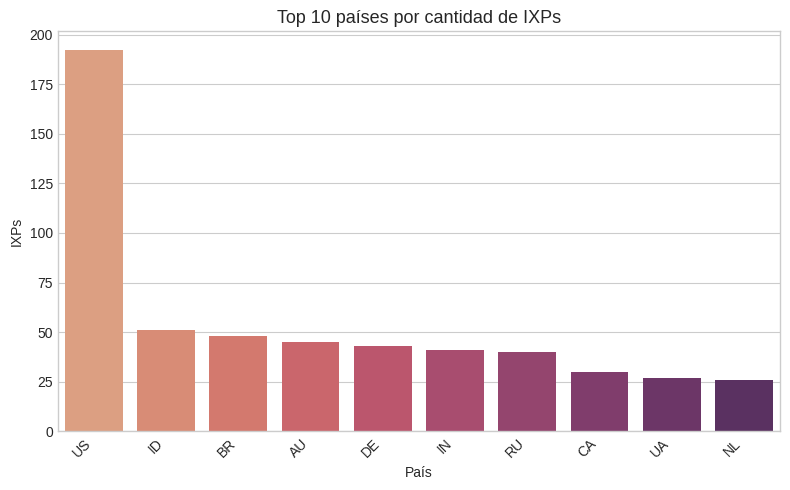
\includegraphics[width=\textwidth]{img/anexoPeeringDB/Top_10_países_por_cantidad_deI_XPs.png}
        \caption{Top 10 países con mayor cantidad de IXPs registrados en PeeringDB.}
        \label{fig:Top_10_países_por_cantidad_deI_XPs}
    \end{subfigure}
    \hfill
    \begin{subfigure}[b]{0.48\textwidth}
        \centering
        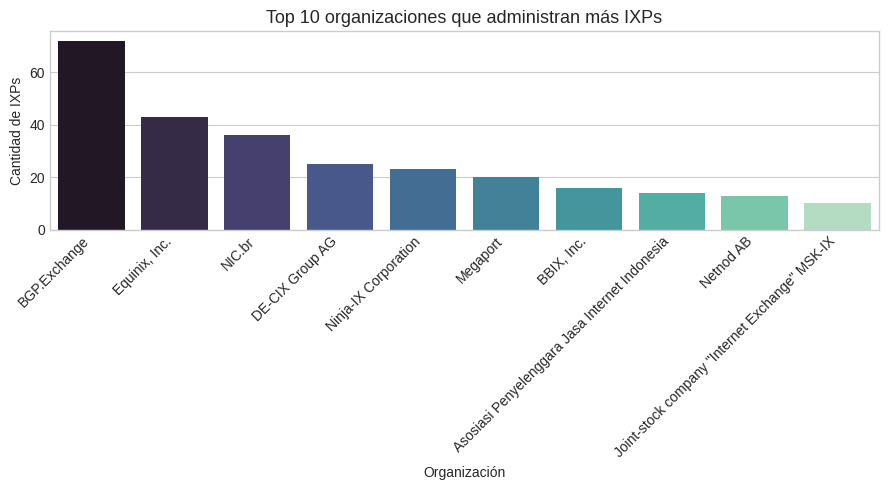
\includegraphics[width=\textwidth]{img/anexoPeeringDB/Top _10_organizaciones_que_administran_mas_IXPs.png}
        \caption{Top organizaciones que administran mayor cantidad de IXPs registrados en PeeringDB.}
        \label{fig:Top_10_org_por_cantidad_deI_XPs}
    \end{subfigure}

    % === 2da fila: figura centrada ===
    \vspace{6mm}
    \begin{subfigure}[b]{0.6\textwidth}
        \centering
        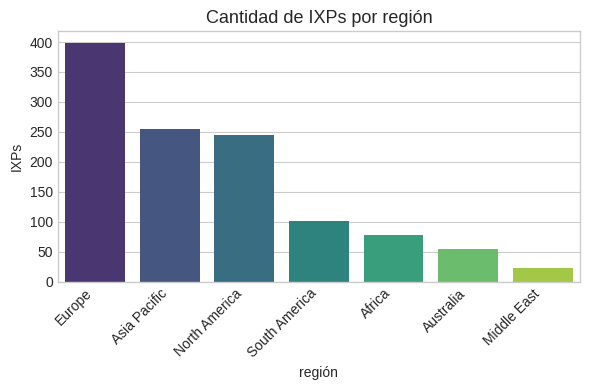
\includegraphics[width=\textwidth]{img/anexoPeeringDB/Cantida_de_IXPs_por_region.png}
        \caption{Cantidad de IXPs por región.}
        \label{fig:Cantida_de_IXPs_por_region}
    \end{subfigure}

    % === Caption general ===
    \caption{Distribución y administración de IXPs registrados en PeeringDB: comparación por país, organización y región geográfica.}
    \label{fig:ixps_peeringdb}
\end{figure}



\begin{table}
\caption{IXPs registrados en Chile según PeeringDB (2024).}
\label{tab:ixps_chile}
\begin{tabular}{l l c}
\toprule
Nombre del IXP & Ciudad & País \\
\midrule
PIT Santiago - PIT Chile & Santiago & CL \\
SCL-IX Chile & Santiago & CL \\
PIT Concepcion - PIT Chile & Concepcion & CL \\
PIT Osorno - PIT Chile & Osorno & CL \\
PIT Temuco - PIT Chile & Temuco & CL \\
PIT Arica - PIT Chile & Arica & CL \\
PIT entel & Santiago & CL \\
BGP.Exchange - Valdivia & Valdivia & CL \\
BGP.Exchange - Santiago & Santiago & CL \\
\bottomrule
\end{tabular}
\end{table}

\section{Tabla Resumen Atributos de ASes de 
trabajo~\cite{BenchmarkingGNN} }

\begin{figure}[h!] % h! = aquí preferentemente
    \centering
    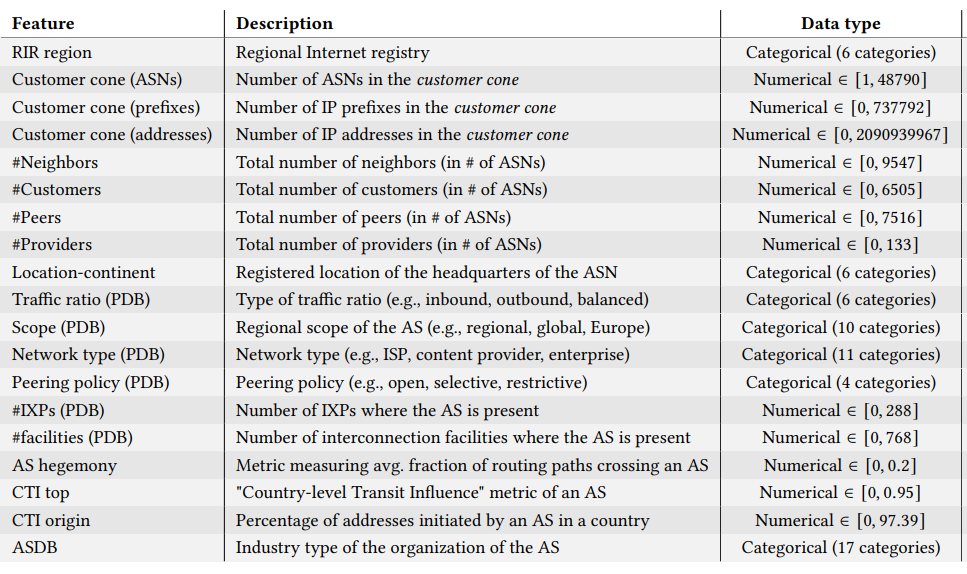
\includegraphics[width=0.9\textwidth]{img/metodologia/tabalAtributosgnnbchn.png}
    \caption{Tabla resumen de atributos del paper ``\textit{Benchmarking Graph Neural Networks for Internet Routing Data}''.}
    \label{tab:as_attr_tabla_bechmark}
\end{figure}



\subsection{Atributos de Sistemas Autónomos utilizados}


\subsection{Análisis de atributos extraídos desde PeeringDB}
Atributos numéricos
Atributos categóricos
\subsection{Análisis del grafo construido}
Grado de salida en datos RIBs
Cantidad de ASes y enlaces en el dataset



\subsection{Análisis temporal de rutas BGP} 







\subsection{Análisis temporal de rutas BGP}
Comparación mensual de longitud de rutas
\subsection{Lista de Sistemas Autónomos Tier-1 considerados}

% TODO: Verificar los Ases esten bien
\begin{table}[ht]
%\centering
\rowcolors{2}{grayA}{grayB}  % ← intercalado entre grisA y grisB

\begin{tabular}{|c|c|c|}
\hline
\textbf{Nombre} & \textbf{Numero} & \textbf{Ubicacion} \\
\hline
Cogent Communications & 174 & Estados Unidos \\
Zayo Group  & 6461 &   Estados Unidos\\
Verizon Enterprise Solutions  & 701 &   Estados Unidos\\
Arelion & 1299 &   Suecia\\
PCCW Global & 3491 & Hong Kong\\
Deutsche Telekom Global Carrier &  	3320 & Alemania\\
Telecom Italia Sparkle & 6762 & Italia\\
AT\&T & 7018 & Estados Unidos\\
Telxius & 12956 &   España\\
Liberty Global & 6830 & Países Bajos\\
Tata Communications & 6453 & India\\
Orange & 5511 & Francia\\
Lumen Technologies & 3356 & Estados Unidos\\
GTT Communications & 3257 &   Estados Unidos\\
NTT Communications & 2914 & Japón\\
Verizon Business & 2828 & Estados Unidos \\
SprintLink & 1239 & Estados Unidos \\
KPN & 286 & Estados Unidos \\
CenturyLink & 209 & Estados Unidos \\
\hline
\end{tabular}
\caption{Lista con Sistemas Autonomos Tier 1}
\label{tab:tier_1_ases}
\end{table}





\subsection{Tabla colectors disponible de RouteViews Project}

\begin{table}[ht]
%\centering
\rowcolors{2}{grayA}{grayB}  % ← intercalado entre grisA y grisB


% FIXME: ARREGLAR TABLA
\begin{tabular}{|c|c|c|}
\hline
\textbf{Nombre} & \textbf{Numero} & \textbf{Ubicacion} \\
\hline
- & - & - \\
- & - & - \\
- & - & - \\
- & - & - \\
\hline
\end{tabular}
\caption{Tabla colectors disponible de RouteViews Project}
\label{tab:tabla_colectors_routeviews}

\end{table}





\subsection{Tabla colectors disponible de RIPE RIS}

% FIXME: Arreglar tabla
\begin{table}[ht]
%\centering
\rowcolors{2}{grayA}{grayB}  % ← intercalado entre grisA y grisB

\begin{tabular}{|c|c|c|}
\hline
\textbf{Nombre} & \textbf{Numero} & \textbf{Ubicacion} \\
\hline
- & - & - \\
- & - & - \\
- & - & - \\
- & - & - \\
- & - & - \\
\hline
\end{tabular}
\caption{Tabla Colectors RIPE RIS}
\label{tab:tabla_colectors_ripe_ris}
\end{table}

------------------











Nose donde poner estas figuras 



Figura~\ref{fig:top_20_as_febrero_numerorelaciones_src} complementaria que presenta el top 20 de ASes según su grado de salida. 

\begin{figure}[H]
    \centering
    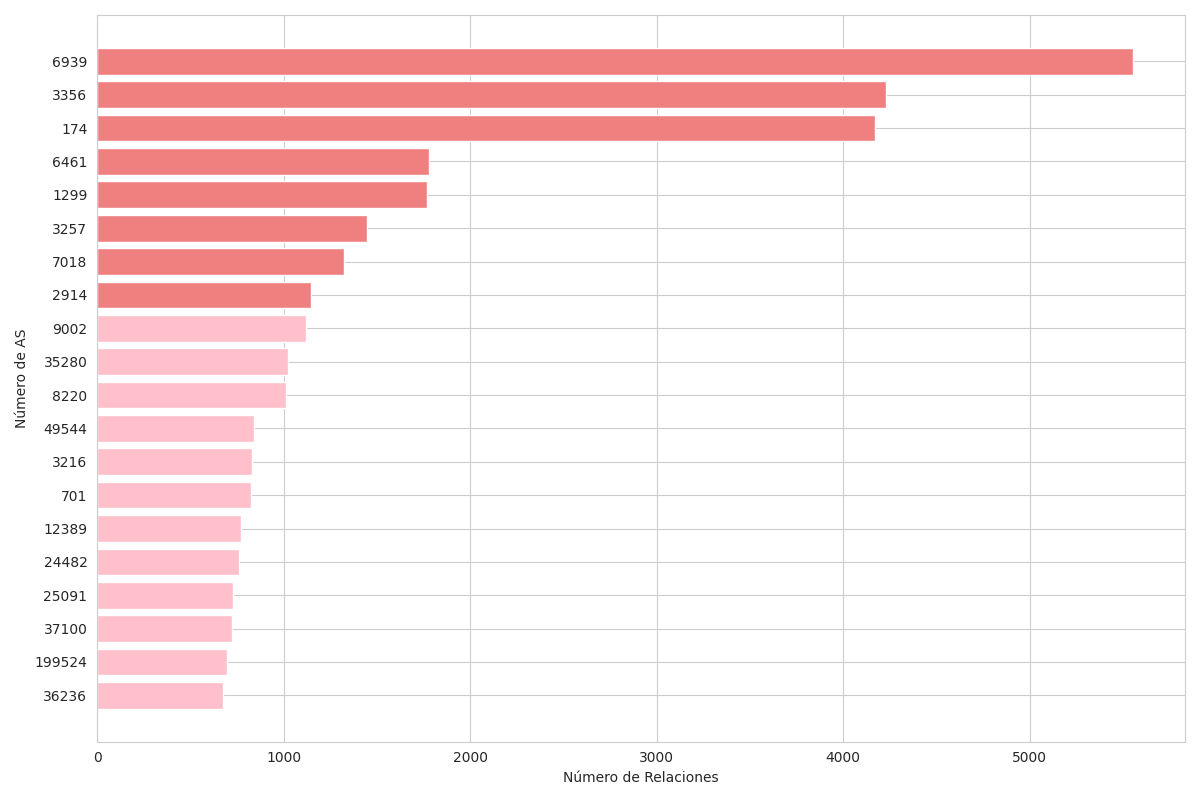
\includegraphics[width=0.9\textwidth]{img/resultados/top_20_as_febrero_numerorelaciones_src.png}
    \caption{Top 20 ASes con mayor número de conexiones (grado), para RIB de febrero 2024.}
\label{fig:top_20_as_febrero_numerorelaciones_src}
\end{figure}


La Figura~\ref{fig:distribucion_as_grado_salida_febrero_comparacion} muestra la distribución del grado de salida de los ASes en febrero, con y sin outliers. Este análisis se enfoca únicamente en las conexiones salientes, a diferencia del informe principal que considera el grado total (entradas y salidas).




\begin{figure}[H]
    \centering

    \begin{subfigure}[b]{0.48\textwidth}
        \centering
        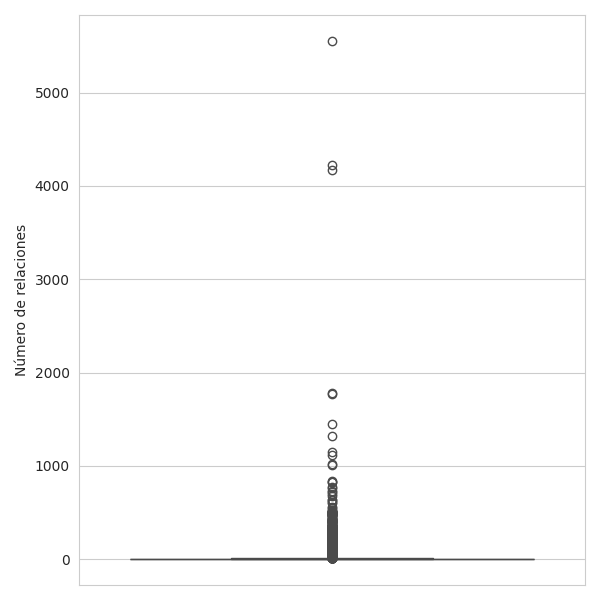
\includegraphics[width=\textwidth]{img/resultados/distribucion_as_grado_salida_febrero_boxplot_con_outliers.png}
        \caption{Con outliers.}
        \label{fig:distribucion_as_grado_salida_febrero_boxplot_con_outliers}
    \end{subfigure}
    \hfill
    \begin{subfigure}[b]{0.48\textwidth}
        \centering
        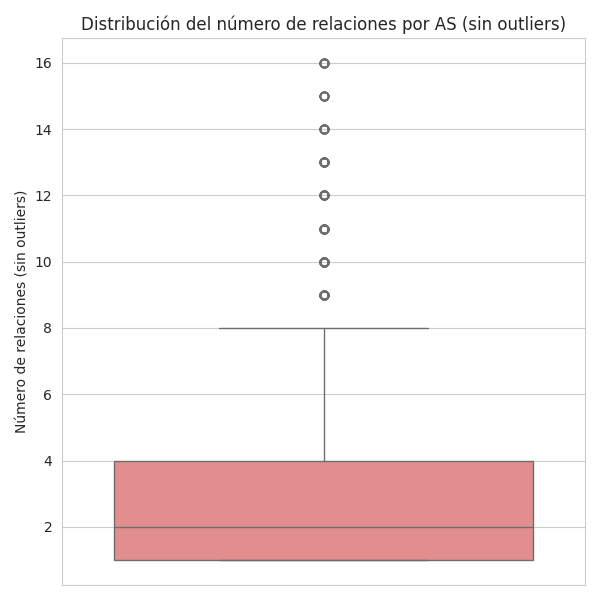
\includegraphics[width=\textwidth]{img/resultados/distribucion_as_grado_salida_febrero_boxplot_sin_outliers.png}
        \caption{Sin outliers.}
        \label{fig:distribucion_as_grado_salida_febrero_boxplot_sin_outliers}
    \end{subfigure}


    \caption{Comparación de la distribución del grado de salida de ASes en febrero, con y sin outliers.}
    \label{fig:distribucion_as_grado_salida_febrero_comparacion}
\end{figure}




La Figura~\ref{fig:comparacion_mensual_largo_paths} muestra la distribución de la longitud de las rutas BGP observadas durante los primeros cuatro meses del año 2024.


\begin{figure}[H]
    \centering
    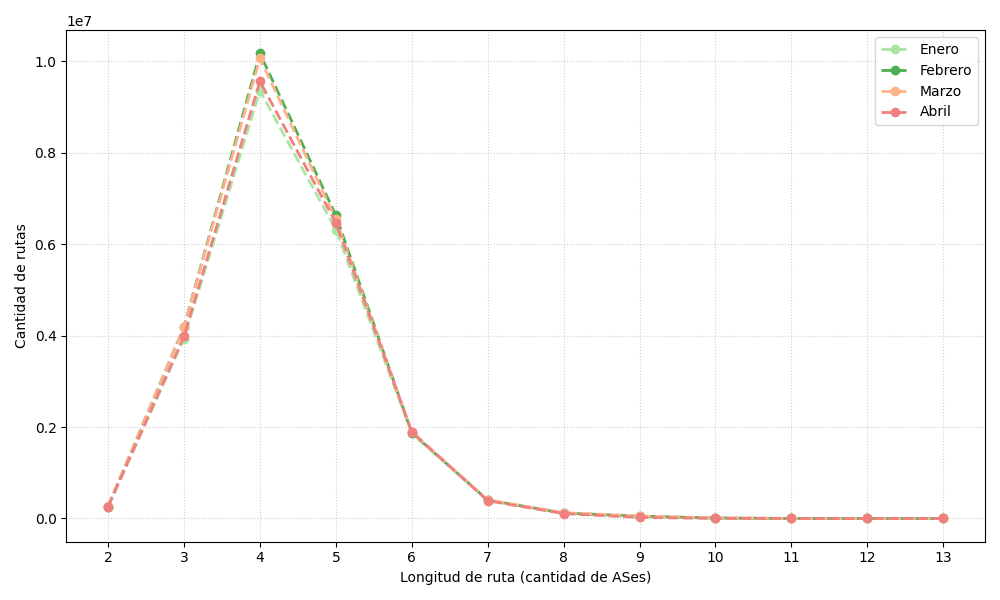
\includegraphics[width=0.8\textwidth]{img/resultados/comparacion_mensual_largo_paths.png}
    \caption{Comparación mensual de la longitud de rutas BGP.}
\label{fig:comparacion_mensual_largo_paths}
\end{figure}











\begin{table}[H]
\centering
\caption{Cantidad de ASes y aristas entre nodos en dataset de evaluacion asrank para los primeros 4 meses del ano}
\begin{tabular}{lcc}
\toprule
\textbf{Mes} & \textbf{Numero de ASes } & \textbf{Enlaces totales} \\
\midrule
Enero   &  76.351 & 499.651 \\
Febrero &  76.415 & 488.777 \\
Marzo   &  76.551 & 492.945 \\
Abril   &  76.644 & 495.601 \\
\end{tabular}
\label{tab:asrank_datasets}
\end{table}



\begin{table}[H]
\centering
\caption{Cantidad de ASes y aristas entre nodos en dataset de evaluacion asrank para los primeros 4 meses del ano}
\begin{tabular}{lcc}
\toprule
\textbf{Mes} & \textbf{Numero de ASes } & \textbf{Enlaces totales} \\
\midrule
Enero   &  76.351 & 499.651 \\
Febrero &  76.415 & 488.777 \\
Marzo   &  76.551 & 492.945 \\
Abril   &  76.644 & 495.601 \\
\end{tabular}
\label{tab:asrank_datasets}
\end{table}








	\section{Configuración experimental} \label{sec:anexo_configuracion_experimentos}


	% 4) Soporte de implementacion
	\section{Fragmentos de código de implementación} \label{sec:anexo_fragmentos_codigo}

Este anexo reúne fragmentos representativos de la implementación utilizada durante el desarrollo de la metodología descrita en el Capítulo~\ref{sec:obtencion_datos_section}. En el cuerpo principal de la tesis se privilegia el uso de pseudocódigo y descripciones de alto nivel; en cambio, aquí se presentan extractos concretos del código para facilitar trazabilidad e interpretación técnica.\\

La organización de este anexo sigue la misma estructura del capítulo de Metodología: obtención de datos, benchmark experimental, construcción del grafo y modelos basados en GNN.\\

\subsection{Obtención de Datos}

\subsubsection{Extracción de rutas BGP con BGPStream}

\begin{lstlisting}[language=Python, caption=Implementación de descarga y filtrado de rutas BGP con BGPStream, label=anxcode:bgpstream_download]
import datetime
import pybgpstream

def downloader(start_date, duration):
    base = int(datetime.datetime.strptime(start_date, "%m/%d/%Y").strftime("%s"))

    stream = pybgpstream.BGPStream()
    stream.add_interval_filter(base, base + int(duration))
    stream.add_filter("record-type", "ribs")
    stream.start()

    path_set = set()
    f = open("data/rib.txt", "w")

    rec = stream.get_next_record()
    while rec:
        elem = rec.get_next_elem()
        while elem:
            path = elem.fields["as-path"]
            if "{" in path or "(" in path:
                elem = rec.get_next_elem()
                continue

            prefix = elem.fields["prefix"]
            if ":" not in prefix and path not in path_set:
                f.write(path.replace(" ", "|") + "\\n")
                path_set.add(path)

            elem = rec.get_next_elem()

        rec = stream.get_next_record()

    f.close()
\end{lstlisting}

\subsubsection{Carga estandarizada de rutas BGP}

\begin{lstlisting}[language=Python, caption=Implementación de importación de rutas BGP desde archivo, label=anxcode:importar_bgp_routes]
bgp_routes = [] 

with open(nombre_archivo, 'r') as archivo:
    for i,linea in enumerate(archivo):
        if i > MAX_NUM_ROUTES:
            break
        numeros = linea.strip().split('|')
        bgp_routes.append(numeros) 

print("[RUTAS BGP]:",bgp_routes[:10])
print("[CANTIDAD PATHS]",len(bgp_routes))
\end{lstlisting}

\subsection{Benchmark Experimental}

\subsubsection{Transformación y limpieza de predicciones}

\begin{lstlisting}[language=Python, caption=Conversión de etiquetas de Gao al formato estándar, label=anxcode:transformacion_estandar_gao]
y_test_prediction_new = []
for i in range(len(y_test_prediction)):
    if y_test_prediction[i] % 2 == 0:
        y_test_prediction_new.append(0)
    elif y_test_prediction[i] == 3:
        y_test_prediction_new.append(2)
    elif y_test_prediction[i] == 1:
        y_test_prediction_new.append(1)
    else:
        y_test_prediction_new.append(-1)

y_test_prediction_new = np.asarray(y_test_prediction_new)
print(len(y_test_prediction_new))
y_test_prediction = y_test_prediction_new
\end{lstlisting}

\begin{lstlisting}[language=Python, caption=Limpieza de relaciones sin ground truth válido, label=anxcode:limpieza_valores_no_encontrados]
x_test_cleaned = np.asarray([np.asarray(x_test[i]) for i in range(len(x_test)) if y_test_prediction[i] != -1])
y_test_cleaned = np.asarray([y_test[i] for i in range(len(y_test)) if y_test_prediction[i] != -1])

y_test_prediction_cleaned = np.asarray([y_test_prediction[i] for i in range(len(y_test_prediction)) if y_test_prediction[i] != -1])
\end{lstlisting}

\subsubsection{Integración de BGP2Vec}

\begin{lstlisting}[language=Python, caption=Inicialización del modelo BGP2Vec, label=anxcode:bgp2vec_init]
bgp2vec = BGP2VEC(model_path = MODELS_PATH,
                  bgp_routes = bgp_routes,
                  rewrite = True,
                  test_limit = test_limit,
                  mode = mode,
                  epochs = epochs)
\end{lstlisting}

\begin{lstlisting}[language=Python, caption=Mapeo de ASN a índices para entrenamiento y prueba en BGP2Vec, label=anxcode:bgp2vec_mapping]
x_training_mapped = []
y_training_filtered = []

for (a, b), y in zip(x_training, y_training):
    a_index = asn_to_index.get(str(a), 0)
    b_index = asn_to_index.get(str(b), 0)
    if a_index == 0 or b_index == 0:
        continue
    x_training_mapped.append([a_index, b_index])
    y_training_filtered.append(y)

x_training_mapped = np.array(x_training_mapped)
y_training_filtered = np.array(y_training_filtered)

x_test_mapped = []
y_test_filtered = []

for (a, b), y in zip(x_test, y_test):
    a_index = asn_to_index.get(str(a), 0)
    b_index = asn_to_index.get(str(b), 0)
    if a_index == 0 or b_index == 0:
        continue
    x_test_mapped.append([a_index, b_index])
    y_test_filtered.append(y)

x_test_mapped = np.array(x_test_mapped)
y_test_filtered = np.array(y_test_filtered)
\end{lstlisting}

\subsection{Construcción del Grafo de Internet}

\subsubsection{Construcción del grafo en formato DGL}

\begin{lstlisting}[language=Python, caption=Clase base para construir el dataset del grafo, label=anxcode:graph_class]
class Graph:
    def __init__(self,dataset_graph_path ,max_paths,debug = False):
        self.debug = debug
        self.nx_graph = None
        self.data_path = dataset_graph_path
        
    def create_topology_from_ribs(self, rib_filename:str,filename_out="edges.csv"):
        ...

    def features_nodes(self,features_filename,filename_out="nodes.csv"):
        ...

    def remove_nodes_degree(self, degree,filename_out="edges.csv"):
        ...
\end{lstlisting}

\subsection{Modelos Basados en GNN}

\subsubsection{Modelos para inferencia con GNN y CNN}

\begin{lstlisting}[language=Python, caption=Implementación de un modelo GCN con distintos decodificadores, label=anxcode:modelo_gcn]
class GCN(nn.Module):
    def __init__(self, in_feats, hidden_feats, out_feats, out_feats_mlp=1, drop=0.3):
        super().__init__()
        self.conv1 = GraphConv(in_feats, hidden_feats)
        self.conv2 = GraphConv(hidden_feats, out_feats)
    
        self.MLP = MLPPredictor(out_feats,out_feats_mlp)
        self.BilinearDecoder = BilinearPredictor(out_feats, 3)
        self.regressor = nn.Linear(out_feats, 1)
        self.drop  = nn.Dropout(drop)

    def encode(self, g, x):
        g = dgl.add_self_loop(g)
        h = self.drop(F.relu(self.conv1(g, x)))
        h = self.conv2(g, h)
        return h

    def decodeDotProduct(self, g, h):
        with g.local_scope():
            g.ndata["h"] = h
            g.apply_edges(fn.u_dot_v("h", "h", "score"))
            return g.edata["score"][:, 0]

    def decodeMLP(self, g, h):
        return self.MLP(g, h)

    def decodeBilinear(self, g, h):
        return self.BilinearDecoder(g, h)

    def forward(self, g, x):
        h = self.encode(g, x)
        out = self.regressor(h).squeeze(-1)
        return out
\end{lstlisting}

\begin{lstlisting}[language=Python, basicstyle=\ttfamily\footnotesize, caption=Mapeo final de ASN a índices para la etapa supervisada, label=anxcode:mapeo_asn_id]
x_training_mapped = []
y_training_filtered = []

for (a, b), y in zip(x_training, y_training):
    a_index = asn_to_index.get(str(a), 0)
    b_index = asn_to_index.get(str(b), 0)

    if a_index == 0 or b_index == 0:
        continue

    x_training_mapped.append([a_index, b_index])
    y_training_filtered.append(y)

x_training_mapped = np.array(x_training_mapped)
y_training_filtered = np.array(y_training_filtered)

x_test_mapped = []
y_test_filtered = []

for (a, b), y in zip(x_test, y_test):
    a_index = asn_to_index.get(str(a), 0)
    b_index = asn_to_index.get(str(b), 0)

    if a_index == 0 or b_index == 0:
        continue

    x_test_mapped.append([a_index, b_index])
    y_test_filtered.append(y)

x_test_mapped = np.array(x_test_mapped)
y_test_filtered = np.array(y_test_filtered)

np.save(PATH + DATA + "x_training_mapped.npy", x_training_mapped)
np.save(PATH + DATA + "y_training_filtered.npy", y_training_filtered)
np.save(PATH + DATA + "x_test_mapped.npy", x_test_mapped)
np.save(PATH + DATA + "y_test_filtered.npy", y_test_filtered)
\end{lstlisting}

\begin{lstlisting}[basicstyle=\ttfamily, caption=Modelo CNN utilizado en el enfoque BGP2Vec, label=anxcode:cnn_bgp2vec_model]
experiment = None
num_classes = len(class_names)
embedding_trainable = False
input_length = 2
embedding_vector_length = embeddings.shape[1]
total_ASNs = embeddings.shape[0]

model = Sequential()
model.add(Embedding(total_ASNs, embedding_vector_length, input_length=input_length,
                    weights=[embeddings], trainable=embedding_trainable))
model.add(Conv1D(filters=32, kernel_size=3, padding='same', activation='relu'))
model.add(Reshape((32, 2)))
model.add(MaxPooling1D(pool_size=2))
model.add(Conv1D(filters=32, kernel_size=3, padding='same', activation='relu'))
model.add(Reshape((32, 16)))
model.add(MaxPooling1D(pool_size=2))
model.add(Flatten())
model.add(Dense(100, activation='relu'))
model.add(Dense(num_classes, activation='softmax'))
\end{lstlisting}

\begin{lstlisting}[basicstyle=\ttfamily, caption=Cálculo de pesos por clase para balanceo, label=anxcode:class_weights_dict]
from sklearn.utils import class_weight
import numpy as np

class_weights = class_weight.compute_class_weight(
                    class_weight='balanced', 
                    classes=np.array(list(range(num_classes))), 
                    y=y_training_filtered)

class_weight_dict = {i: w for i, w in enumerate(class_weights)}
print('[class_weights_dict]:', class_weight_dict)
\end{lstlisting}




\end{appendixs}


\end{document}
